\documentclass[11pt,a4paper]{article}

\usepackage{amsfonts,amssymb,amsmath}
\usepackage[margin=1in]{geometry}
\usepackage[none]{hyphenat}
\usepackage{graphicx}
\usepackage{fancyhdr}
\usepackage{float}
\usepackage{color}
\usepackage{xcolor}
\usepackage{tikz}
\usepackage{polynom}
\usepackage{bigints}
\usepackage{esint}
\usepackage[nottoc,notlot,notlof]{tocbibind}

\usetikzlibrary{quotes,angles,graphs,patterns,fadings,arrows.meta,shapes,trees,bending}

\parindent 0ex
\setlength{\parskip}{0.55\baselineskip}
% Displays carry their own skips; with a non-zero \parskip on top of them,
% consecutive displays drift apart. Tighten them so a derivation reads as one
% argument rather than as a column of disconnected formulae.
\setlength{\abovedisplayskip}{0.5\baselineskip}
\setlength{\belowdisplayskip}{0.5\baselineskip}
\setlength{\abovedisplayshortskip}{0.25\baselineskip}
\setlength{\belowdisplayshortskip}{0.25\baselineskip}

\pagestyle{fancy}
\fancyfoot[C]{\thepage}
\fancyhead{}
\fancyhead[R]{\rightmark}
\renewcommand{\headrulewidth}{0pt}

% Theorem environments. The source declared none: its 125 examples, 91
% solutions, 21 definitions and 30 theorems were set as red bold text with the
% number typed by hand, so LaTeX numbered nothing and inserting an example meant
% renumbering the rest of the subsection.
\usepackage{amsthm}
\theoremstyle{definition}
% One shared counter running section.subsection.n, as in the other courses here.
\newtheorem{thm}{Theorem}[subsection]
\newtheorem{defn}[thm]{Definition}
\newtheorem{exa}[thm]{Example}
\newtheorem{prop}[thm]{Proposition}
\newtheorem{coro}[thm]{Corollary}
\newtheorem{lem}[thm]{Lemma}
\newtheorem{result}[thm]{Result}
\newtheorem{exe}[thm]{Exercise}
\newtheorem*{note}{Note}
\newtheorem*{remark}{Remark}
\newtheorem{problemx}{Problem}[subsection]
\newenvironment{problem}{\begin{problemx}}{\end{problemx}}
\newenvironment{solution}
  {\renewcommand{\qedsymbol}{}\begin{proof}[\textit{Solution}.]}
  {\end{proof}}
\usepackage{enumitem}
% A heading that is legal inside a theorem body, a list or a float, where
% \subsubsection is not. Same weight as \subsubsection* so the two read alike.
\newcommand{\subhead}[1]{%
  \par\medskip\noindent\textbf{#1}\par\nobreak\smallskip}

\begin{document}

% Title page depersonalised for the web, as with every other course here: no
% university, no lecturers, no author, no year. The identity kept below is the
% divergence theorem, which ties the multiple integration of the middle sections
% to the vector analysis of the later ones.
\begin{titlepage}
\begin{center}
\vspace*{3cm}
{\Huge\bfseries Advanced Calculus}\\[1.2cm]
{\large Lecture Notes}\\[2.5cm]
\line(1,0){300}\\[1.5cm]
$$\iiint_V \nabla\cdot\underline{F}\,dV = \iint_S \underline{F}\cdot\underline{n}\,dS$$
\end{center}
\end{titlepage}

\tableofcontents
\thispagestyle{empty}
\clearpage
\setcounter{page}{1}

{\color[wave]{485}\section{Functions Of Several Variables}}

\begin{defn}


A function $f$ of two variables is a correspondence that associates with each pair $(x,y)\in D$, a unique real number, denoted $f(x,y)$. $$z = f(x,y)$$
\begin{align*}
z & - \text{dependent variable}\\
x,y & - \text{independent variables}\\\\
\end{align*}

Examples of functions of two or three variables
\begin{enumerate}
\item[$-$] Volume of Cylinder $\displaystyle{V = \pi r^2 h}$

\item[$-$] Ideal gas law $\hspace{0.4cm}\displaystyle{P = \frac{RT}{V}}$

\item[$-$] $z = f(x,y) = \sqrt{1 - x^2 - y^2}$
\begin{align*}
\text{Domain} & = \{(x,y)\hspace{0.1cm}|\hspace{0.2cm} x^2 + y^2 \leq 1\}\\\\
\text{Range of}\hspace{0.2cm} z & = \{z\hspace{0.1cm}|\hspace{0.2cm} 0\leq z \leq 1\}\\
                  & = [0,1]\\
\end{align*}
\end{enumerate}

In $3D$, the set of points $(x,y,z)$ such $z = 1 - x^2 - y^2$
$$\implies \hspace{0.5cm} z^2 = 1 - x^2 - y^2$$

$$ x^2 + y^2 + z^2 = 1 \hspace{0.2cm}\text{i.e Sphere with radius 1}$$

$$z = \sqrt{1 - x^2 - y^2}\hspace{0.3cm}\text{is a hemisphere of radius}$$

% DIAGRAM 1

\begin{figure}[H]
\centering
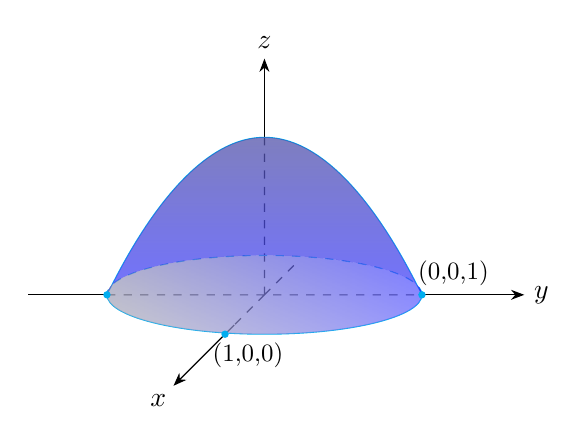
\begin{tikzpicture}[=>stealth]
\draw[dashed](-2,0,0)--(2,0,0)
(0,0,0)--(0,2,0)
(0,0,0)--(0,0,1)
(0,0,0)--(0,0,-1);
\draw[-Stealth](0,2,0)--(0,3,0)node[above]{$z$};
\draw[-Stealth](2,0,0)--(3.3,0,0)node[right]{$y$};
\draw[-Stealth](0,0,1)--(0,0,3);
\draw(-3,0,0)--(-2,0,0);
\draw[cyan](0,2)parabola(2,0)
(0,2)parabola(-2,0);
\draw[cyan](-2,0)arc(180:360:2cm and 0.5cm);
\draw[dashed,cyan](2,0)arc(0:180:2cm and 0.5cm);
%\path[fill=cyan,opacity=0.5](0,0)circle(2cm and 0.5cm)--(2,0)parabola[bend at end](0,2)--(0,2)parabola(-2,0);
\shade[top color=blue, opacity=0.5](0,2)parabola(2,0)--(2,0)arc(360:-180:2cm and 0.5cm)--(-2,0)parabola[bend at end](0,2)--cycle;
\shade[bottom color=blue,opacity=0.5](0,2)parabola(2,0)--(2,0)arc(0:180:2cm and 0.5cm)--(-2,0)parabola[bend at end](0,2)--cycle;
\shade[right color=blue,opacity=0.4](0,0)circle(2cm and 0.5cm);
\draw(2.4,0,0)node[above,scale=0.9]{(0,0,1)}
(2,0,0)node[shape=circle,scale=0.01cm, fill=cyan]{}
(-2,0,0)node[shape=circle,scale=0.01cm,fill=cyan]{}
(0,0,1.3)node[shape=circle,scale=0.01cm,fill=cyan]{}
(0,0,3.5)node[]{$x$}
(0,0,2)node[right,scale=0.9]{(1,0,0)};
\end{tikzpicture}
\end{figure}
\end{defn}

{\color[wave]{485}\subsection{Level Curves}}
Another useful method of describing a function of two variables consists of sketching in the $xy-$ plane, the groups of $f(x,y) = K$ (a constant) for various values of $K$. The graphs so obtained are called level curves of $f$.\\ \textit{N.B} As a point $(x,y)$ moves on a level curve the values of $f(x,y)$ are constant.


For the function $z = \sqrt{1 - x^2 - y^2}$

\begin{align*}
\text{Let}\hspace{0.5cm} K & = \sqrt{1 - x^2 - y^2}\\
K^2 & = 1 - x^2 - y^2\\
x^2 + y^2 & = 1 - K^2
\end{align*}

\begin{align*}
K & = 0 \hspace{1cm} x^2 + y^2 = 1\\
K & = 1 \hspace{1cm} x^2 + y^2 = 0\\
K & = 2 \hspace{1cm} x^2 + y^2 = -3\hspace{0.5cm}\text{undefined}\\
\end{align*}

% DIGRAM 2

\begin{figure}[H]
\centering
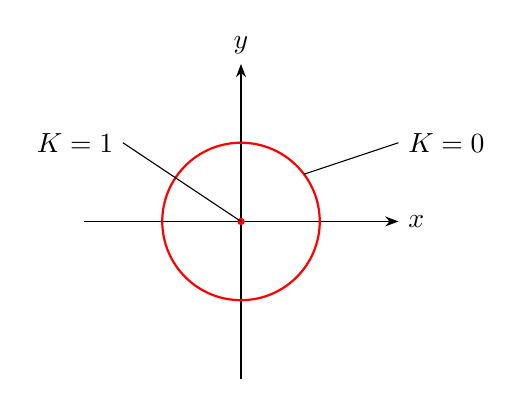
\begin{tikzpicture}[=>stealth]
\draw[-Stealth](-2,0)--(2,0)node[right]{$x$};
\draw[-Stealth](0,-2)--(0,2)node[above]{$y$};
\draw(0,0)node[shape=circle,fill=red,scale=0.01cm]{};
\draw[thick,red](0,0)circle [radius=1cm];
\draw(0,0)--(-1.5,1)node[left]{$K=1$};
\draw(0.8,0.6)--(2,1)node[right]{$K=0$};
\end{tikzpicture}
\end{figure}

\begin{exa}


Given a function $g(x,y) = \sqrt{9 - x^2 - 2y^2}$
\begin{enumerate}
\item Find the domain and range.

\item Sketch the level curves of $g$
\end{enumerate}
\end{exa}

\begin{solution}
\begin{enumerate}
\item $\displaystyle{g(x,y)\geq 0\implies 9 - x^2 -2y^2\geq 0 \implies x^2 + 2y^2 \leq 9}$

\begin{align*}
\text{Domain}\hspace{0.5cm} D & = \big\{(x,y)\hspace{0.1cm} |\hspace{0.1cm} x^2 + 2y^2 \leq 9\big\}\\\\
\text{Range}\hspace{0.5cm} R & = \big\{z \hspace{0.1cm} |\hspace{0.1cm} 0\leq z \leq 3\big\}\\\\
\end{align*}

\item Level curves
$$K = \sqrt{9 - x^2 - 2y^2}$$

$$x^2 + 2y^2 = 9 - K^2$$

\begin{align*}
K & = 0 \hspace{1cm} x^2 + 2y^2 = 9\\
K & = 1 \hspace{1cm} x^2 + 2y^2 = 8\\
\vdots &\\
K & = 3 \hspace{1cm} x^2 + 2y^2 = 0\\
\end{align*}

% DIAGRAM 3

\begin{figure}[H]
\centering
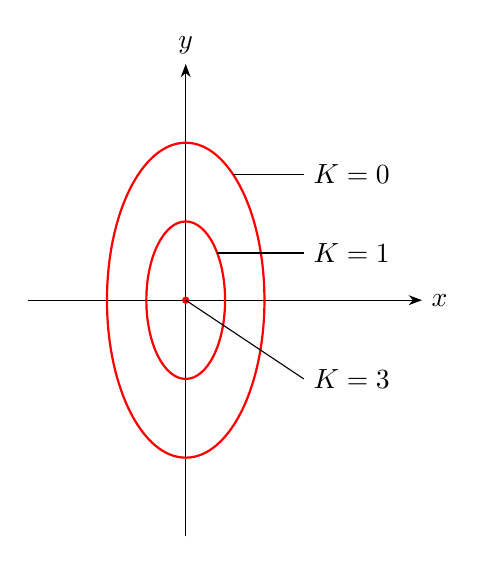
\begin{tikzpicture}[=>stealth]
\draw[-Stealth](0,-3)--(0,3)node[above]{$y$};
\draw[-Stealth](-2,0)--(3,0)node[right]{$x$};
\draw(0,0)node[shape=circle,fill=red,scale=0.01cm]{};
\draw[thick,red](0,0)ellipse[x radius=0.5cm, y radius=1cm];
\draw[thick,red](0,0)ellipse[x radius =1cm,y radius=2cm];
\draw(0,0)--(1.5,-1)node[right]{$K=3$};
\draw(0.6,1.6)--(1.5,1.6)node[right]{$K=0$};
\draw(0.4,0.6)--(1.5,0.6)node[right]{$K=1$};
\end{tikzpicture}
\end{figure}
\end{enumerate}
\end{solution}

\begin{exa}


Find the domain of $f$ if $$f(x,y,z) = \ln (z-y) + xy\sin z$$
\end{exa}

\begin{solution}


$\displaystyle{D = \big\{(x,y,z) \hspace{0.1cm} |\hspace{0.1cm} z - y > 0\big\}}$

% DIAGRAM 4

\begin{figure}[H]
\centering
\begin{tikzpicture}[=>stealth]
\draw[-Stealth](0,0,0)--(3,0,0)node[right]{$y$};
\draw[-Stealth](0,0,0)--(0,3,0)node[above]{$z$};
\draw[-Stealth](0,0,0)--(0,0,3);
\draw(0,0,3.5)node[]{$x$};
\draw[dashed](-1,0,0)--(0,0,0)
(0,0,-1)--(0,0,0);
\end{tikzpicture}
\end{figure}

$\displaystyle{R = \big\{\mathbb{R}\big\}}$
\end{solution}


{\color[wave]{485}\subsection{Limits and Continuity}}

\begin{defn}


The function $f(x,y)$ is said to have a limit at the point $P_0(x_0,y_0)$ and we can write $$ \lim\limits_{(x,y) \longrightarrow (x_0,y_0)}f(x,y) = L$$
If for each positive $\varepsilon$, there exists a $\delta$ that if $$0 < (x-x_0)^2 + (y-y_0)^2 <\delta^2, \hspace{0.3cm}\text{then}\hspace{0.3cm} \big|f(x,y) - L\big| < \varepsilon$$

i.e the point $P(x,y)$ lies inside a certain circle of radius $\delta$, and centre $P_0(x_0,y_0)$.
\end{defn}


\begin{defn}


The function $f(x,y)$ is continuous at $P_0(x_0,y_0)$ if 
\begin{enumerate}
\item $f$ must be defined

\item $\displaystyle{\lim\limits_{(x,y)\longrightarrow (x_0,y_0)} = L}$

\item $\displaystyle{\lim\limits_{(x,y)\longrightarrow (x_0,y_0)} = f(x_0,y_0)}$
\end{enumerate}

The function $f$ is continuous in the set $S$ if it is continuous at every point of $S$.
\end{defn}


\begin{exa}


$f(x,y) = 
\begin{cases}
3xy & (x,y) \neq (1,2)\\\\
0 & (x,y) = (1,2)\\
\end{cases}
$


\begin{enumerate}
\item $f(x,y)$ is defined at $(1,2)$

\item $\displaystyle{\lim\limits_{(x,y)\rightarrow (1,2,)}f(x,y) = 6}$

\item $\displaystyle{ f(1,2) = 0\neq \lim\limits_{(x,y)\rightarrow (1,2,)}f(x,y)}$
\end{enumerate}

Condition 3 is violated


But
$f(x,y) = 
\begin{cases}
3xy & (x,y) \neq (1,2)\\\\
6 & (x,y) = (1,2)\\
\end{cases}
$


$\lim\limits_{(x,y)\rightarrow (1,2,)}f(x,y) = 6 = f(1,2)$. Then $f(x,y)$ is continuous.
\end{exa}


\begin{exa}


Let $\displaystyle{f(x,y) = \frac{xy}{x^2 + y^2}\hspace{0.1cm}, \hspace{0.4cm} (x,y) \neq (0,0)}$.
Does the function have a limit as $P \longrightarrow (0,0)$?
\end{exa}


\begin{solution}


Denote $f(P)$ for $f(x,y)$. Let $P$ approach $(0,0)$ along the line $y = mx$

\begin{align*}
f(P) & = \frac{x(mx)}{x^2 + (mx)^2}\hspace{1cm} x\neq 0\\\\
& = \frac{m x^2}{x^2(1 +m^2)}\\\\
& = \frac{m}{1 + m^2}
\end{align*}

Hence on each line through origin $f(p)$ is constant.


For $y = x$, $m = 1$ and $f(P) = \dfrac{1}{2}$ as $P \longrightarrow (0,0)$


For $y = 2x$, $m = 2$ and $f(P) = \dfrac{2}{5}$ as $P \longrightarrow (0,0$


Since $\dfrac{1}{2} \neq \dfrac{2}{5}$ , no unique $L$ that will define 1. Hence the function does not have a limit (or does not exist).
\end{solution}


\begin{exa}


Given the functions
\begin{enumerate}
\item $\displaystyle{z = \frac{\sin (x+y)}{x + y}}\hspace{0.8cm}$ hint: $\displaystyle{\lim_{x\longrightarrow 0} \frac{\sin x}{x}=1}$

\item $\displaystyle{z = \frac{xy}{x^2 + y^2}}$
\end{enumerate}
Investigate whether continuous at the origin.\
\end{exa}


\subhead{Extension to Three of More Variables}

$\displaystyle{\lim_{(x,y,z)\rightarrow (a,b,c)}f(x,y,z) =L}$


Means the values of $f(x,y,z)$ approach $L$ as the point approaches $(a,b,c)$.


For example, the function $$f(x,y,z) = \frac{1}{x^2 + y^2 + z^2 - 1}$$
is a rational function of three variables and it is continuous everywhere in $\mathbb{R}^3$ except when $x^2 + y^2 + z^2 = 1$. It is discontinuous on the sphere with centre $(0,0,0)$ and radius 1.


{\color[wave]{485}\subsection{Directional Derivatives and Gradient Vector}}
Recall
$$f_x(x_0,y_0) = \lim_{h\longrightarrow 0} \frac{f(x_0 + h, y_0) - f(x_0,y_0)}{h}$$

$$f_x(x_0,y_0) = \lim_{h\longrightarrow 0} \frac{f(x_0, y_0 +h) - f(x_0,y_0)}{h}$$

represent the rates of change of $z$ in the $x$ and $y$ directions $(\textbf{i}, \textbf{j})$.


\begin{defn}


The directional derivatives of $f$ at $(x_0,y_0)$ in the direction of a  unit vector $u = \langle a, b\rangle = a\,\textbf{i} + b\, \textbf{j}$ is 
$$D_u\hspace{0.1cm} f(x_0,y_0) = \lim_{h\longrightarrow 0} \frac{f(x_0 + h_a, y_0+h_b) - f(x_0,y_0)}{h}$$
\end{defn}


\begin{thm}


If the function $f$ is a differentiable function of $x$ and $y$, then $f$ has a directional derivative in the direction of any unit vector $u = \langle a, b \rangle$ $$D_u\hspace{0.1cm}f(x,y) = f_x(x,y) a + f_y(x,y) b$$
\end{thm}


\begin{exa}


Given $f(x,y) = x^3 -3xy + 4y^2$, find the directional derivative in the direction of $\theta = \dfrac{\pi}{6}$ , $u$ is unit


$f_x = 3x^2 -3y$\hspace{0.2cm}and \hspace{0.2cm} $f_y = -3x + 8y$

% DIAGRAM 5

\begin{figure}[H]
\centering
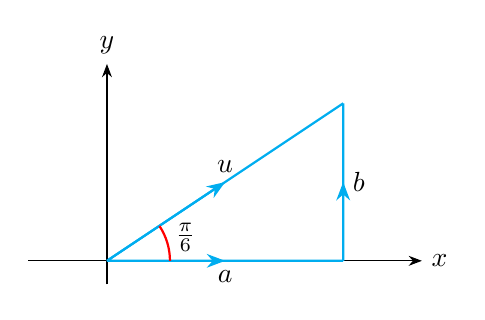
\begin{tikzpicture}[=>stealth]
\draw[-Stealth](-1,0)--(4,0)node[right]{$x$};
\draw[-Stealth](0,-0.3)--(0,2.5)node[above]{$y$};
\draw[thick,cyan,-Stealth](0,0)--(1.5,1);
\draw[thick,cyan,-Stealth](3,0)--(3,1);
\draw[thick,cyan,-Stealth](0,0)--(1.5,0);
\draw[thick,cyan](0,0)--(3,0)
(3,0)--(3,2)
(0,0)--(3,2);
\draw(1.5,0)node[below]{$a$}
(3,1)node[right]{$b$}
(1.5,1)node[above]{$u$};
\coordinate (a) at (0.5,0);
\coordinate (b) at (0,0);
\coordinate (c) at (0.5,0.33);
\draw
pic[thick,draw=red,-,angle radius=0.8cm,"$\frac{\pi}{6}$",angle eccentricity = 1.3]{angle=a--b--c};
\end{tikzpicture}
\end{figure}

$$\sin \frac{\pi}{6} = \frac{b}{1}\hspace{0.5cm}, \hspace{0.5cm} \cos \frac{\pi}{6}= \frac{a}{1}$$

\begin{align*}
D_u f(x,y) & = f_x(x,y)\,a + f_y(x,y)\,b\\
& = \big(3x^2 - 3y\big) \cos \frac{\pi}{6} + \big(-3x + 8y\big) \sin \frac{\pi}{6}
\end{align*}

\begin{align*}
D_u (1,2) & = \big(3x^2 - 3y\big) \frac{\sqrt{3}}{2} + \big(-3x + 8y\big) \frac{1}{2}\\
& = \frac{13 - 3\sqrt{3}}{2}\\\\
\end{align*}
\end{exa}

\subhead{Gradient Vector}


\begin{defn}


If $f$ is a function of two variables $x$ and $y$, then the gradient vector $\nabla f$ is defined as 
$$\nabla f = \frac{\partial f}{\partial x}\,\textbf{i} +\frac{\partial f}{\partial y}\,\textbf{j} = f_x\, \textbf{i} + f_y\,\textbf{j} $$

From theorem 1, the directional derivative can be rewritten as the product of two variables

\begin{align*}
D_u\hspace{0.1cm}f(x,y) & = f_x(x,y) a + f_y (x,y) b\\
& = \langle f_x , f_y\rangle \cdot \langle a,b\rangle\\
& = (f_x\,\textbf{i} + f_y\,\textbf{j}) \cdot (a\,\textbf{i} + b\,\textbf{j})\\\\
\implies \hspace{1cm} D_u\hspace{0.1cm}f(x,y) & = \nabla f\cdot\overrightarrow{u}\\\\
\end{align*}
\end{defn}

\begin{exa}


If $\displaystyle{f(x,y) = \sin x + e^{xy}}$, find $\nabla f$.
\end{exa}


\begin{solution}
\begin{align*}
\nabla f & = f_x\,\textbf{i} + f_y\, \textbf{j}\\
& = \big(\cos x + ye^{xy}\big)\,\textbf{i} + \big(xe^{xy}\big)\,\textbf{j}\\
& = \langle \cos x + ye^{xy}, xe^{xy}\rangle\\\\
\implies\hspace{1cm} \nabla f (0,1) & = \langle 2,0\rangle\\
\end{align*}
\end{solution}

\begin{exa}


Find the directional derivative of $f(x,y) = x^2y^3 -4y$ at the  point $(2,-1)$ in the  direction of the vector $V = 2\,\textbf{i} + 5\,\textbf{j}$.
\end{exa}


\begin{solution}
\begin{align*}
\nabla f (x,y) & = f_x\,\textbf{i}+ f_y\,\textbf{j}\\
& = 2xy^3\,\textbf{i} + \big(3x^2y^2 -4\big)\,\textbf{j}\\\\
\implies \hspace{1cm} \nabla f (2,-1) & = -4\,\textbf{i}+ 8\,\textbf{j}
\end{align*}

$$\overrightarrow{u} = \frac{\overrightarrow{V}}{\big|\overrightarrow{V}\big|} = \frac{2\,\textbf{i} + 5\,\textbf{j}}{\sqrt{29}} = \frac{2}{\sqrt{29}}\,\textbf{i} + \frac{5}{\sqrt{29}}\, \textbf{j}$$

\begin{align*}
D_uf(2,-1) & = \nabla f (2,-1)\cdot\overrightarrow{u}\\
& = \big( - 4\,\textbf{i} + 8\,\textbf{j}\big)\cdot \bigg(\frac{2}{\sqrt{29}}\,\textbf{i} + \frac{5}{\sqrt{29}}\,\textbf{j}\bigg)\\\\
& = \frac{-8}{\sqrt{29}} + \frac{40}{\sqrt{29}}= \frac{32}{\sqrt{29}}\\\\
& = \frac{32\sqrt{29}}{29}\\
\end{align*}
\end{solution}

\begin{defn}


The directional derivative of $f$ at $(x_0,y_0,z_0)$ in the directional of a unit a vector $\overrightarrow{u} = \langle a, b, c\rangle$ is 
$$D_u\hspace{0.1cm}f(x_0,y_0,z_0) = \lim_{h\longrightarrow 0} \frac{f(x_0 + h_a, y_0 + h_b, z_0 + h_c) - f(x_0,y_0,z_0)}{h}$$
\end{defn}


\begin{exa}


Given $f(x,y,z) = x\sin yz$, find the 
\begin{enumerate}
\item the gradient of $f$

\item the directional derivative of $f$  at $(1,3,0)$ in the direction of $V = \textbf{i} + 2\textbf{j} -\textbf{k}$
\end{enumerate}
\end{exa}

\begin{solution}


$\displaystyle{\overrightarrow{u} = \frac{\overrightarrow{V}}{\big|\overrightarrow{V}\big|}=\frac{1}{\sqrt{6}}\big(\textbf{i} + 2\,\textbf{j} - \textbf{k}\big)}$

\begin{align*}
\nabla f & = f_x\,\textbf{i} + f_y\,\textbf{j} + f_z\,\textbf{k}\\\\
& = \big(\sin yz\big)\,\textbf{i} + \big( xz\cos yz\big)\,\textbf{j} + \big(xy\cos yz\big)\,\textbf{k}\\\\
\implies \hspace{1cm} \nabla f(1,3,0) & = 3\,\textbf{k} 
\end{align*}

\begin{align*}
D_u f(1,3,0) & = \nabla f(1,3,0)\cdot\overrightarrow{u}\\
& = 3\,\textbf{k}\cdot \Big(\frac{1}{\sqrt{6}}\big(\,\textbf{i} + 2\,\textbf{j} - \textbf{k}\big)\Big)\\\\
& = - \sqrt{\dfrac{3}{2}}\\\\
\end{align*}
\end{solution}

{\color[wave]{485}\subsection{Maximising the Directional Derivative}}
Suppose that we have a functional of two or three variables and we consider all possible directional derivatives of $f$ at a given point.


{\textcolor{blue}{Question:}} In which direction does $f$ change fastest.


\begin{thm}


Suppose $f$ is a differentiable  function of 2 or 3 variables, the maximum value of the directional derivative.
$D_u\hspace{0.1cm} f\big(\overrightarrow{x}\big)$ is $\big|\nabla f\big(\overrightarrow{x}\big)\big|$ and it occurs when $\overrightarrow{u}$ has the same direction as the gradient vector.


{\color[wave]{485}{Proof}}
\begin{align*}
D_u f & = \nabla f\cdot\overrightarrow{u}\\
      & = \big|\nabla f\big|\hspace{0.1cm}\big|\overrightarrow{u}\big|\hspace{0.1cm} \cos \theta\\
      & = \big|\nabla f\big|\cos \theta
\end{align*}
where $\theta$ is the angle between $\nabla f$ and $\overrightarrow{u}$.


Therefore, the maximum value of $D_u f$ is $\big|\nabla f\big|$ and it occurs when $\theta = 0$.


Direction derivative is maximum in the direction of the gradient vector, zero in directions orthogonal to the gradient vector and minimum in the direction opposite the gradient vector.

% DIAGRAM 6

\begin{figure}[H]
\centering
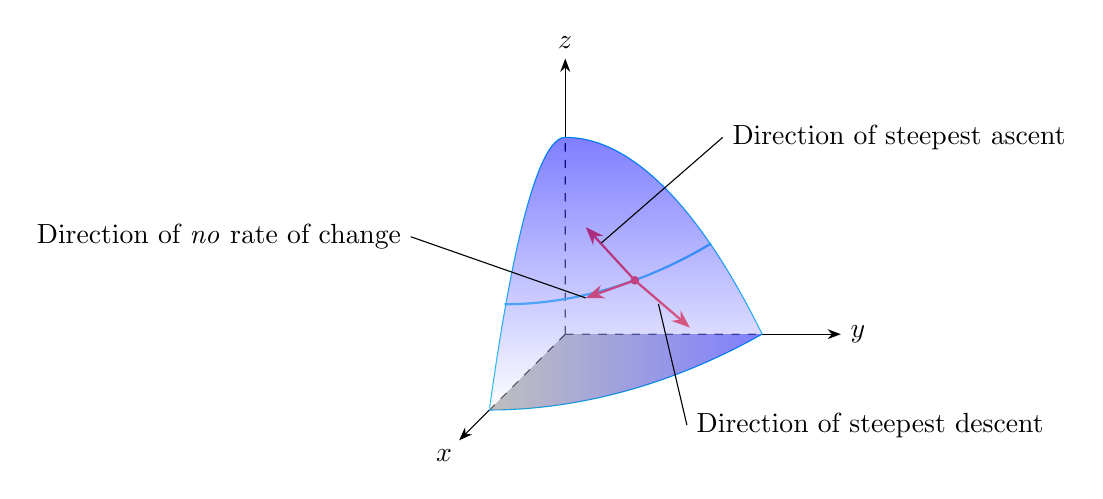
\begin{tikzpicture}[=>stealth]
\draw[-Stealth](2.5,0,0)--(3.5,0,0)node[right]{$y$};
\draw[-Stealth](0,2.5,0)--(0,3.5,0)node[above]{$z$};
\draw[-Stealth](0,0,2.5)--(0,0,3.5);
\draw(0,0,4)node[]{$x$};
\draw[dashed](0,0,0)--(2.5,0,0)
(0,0,0)--(0,2.5,0)
(0,0,0)--(0,0,2.5);
\draw[cyan](2.5,0,0)parabola[bend at end](0,0,2.5)
(0,0,2.5)parabola[bend at  end](0,2.5,0)
(2.5,0,0)parabola[bend at end](0,2.5,0);
\draw[thick,cyan](0,1.15,2)parabola(1.85,1.15,0);
\draw(2,1.8,2.9)node[shape=circle,fill=red,draw=red,scale=0.01cm]{};
\draw[-Stealth,thick,red](2,1.8,2.9)--(1.3,2.4,2.7);
\draw[-Stealth,thick,red](2,1.8,2.9)--(2.7,1.2,2.9);
\draw[-Stealth,thick,red](2,1.8,2.9)--(1.8,2,4);
\shade[top color=blue,opacity=0.5](0,2.5,0)parabola(2.5,0,0)--(2.5,0,0)--(0,0,0)--(0,2.5,0)--cycle
(0,2.5,0)parabola(0,0,2.5)--(0,0,2.5)--(0,0,0)--(0,2.5,0)--cycle;
\shade[right color=blue,opacity=0.5](2.5,0,0)parabola[bend at end](0,0,2.5)--(0,0,2.5)--(0,0,0)--(2.5,0,0)--cycle;
\draw(1.5,2.2,2.7)--(2,2.5,0)node[right]{Direction of steepest ascent};
\draw(1.8,2,4)--(-1,2.2,2.5)node[left]{Direction of \textit{no} rate of change};
\draw(2.3,1.5,2.9)--(2.7,0,3)node[right]{Direction of steepest descent};
%\shade[top color=blue,opacity=0.4](0,2.5,0)parabola(2.5,0,0)--(2.5,0,0)parabola[bend at end](0,0,2.5)--(0,0,2.5)parabola[bend at end](0,2.5,0)--cycle;
\end{tikzpicture}
\end{figure}
\end{thm}

\begin{exa}
\begin{enumerate}
\item If $f(x,y ) = xe^y$ , find the rate of change of $f$ at the point $P(2,0)$ in the directional of $Q\big(1/2,2\big)$.

\item In what direction does $f$ have the max rate of change? What is that max?
\end{enumerate}
\end{exa}

\begin{solution}
\begin{enumerate}
\item $\displaystyle{\nabla f = f_x\,\textbf{i} + f_y\,\textbf{j} = e^y\,\textbf{i} + xe^y\,\textbf{j}}$

$\implies \hspace{1cm}\displaystyle{\nabla f(2,0) = \textbf{i} + 2\,\textbf{j}}$

The unit vector $\displaystyle{\overrightarrow{PQ} = \langle -1.5,2\rangle}$ is $\displaystyle{\overrightarrow{u} = \bigg\langle \dfrac{-3}{5},\dfrac{4}{5}\bigg\rangle}$

\begin{align*}
D_u f(2,0) & = \langle 1,2\rangle\cdot \bigg\langle \dfrac{-3}{5},\dfrac{4}{5}\bigg\rangle\\
& = 1\\
\end{align*}

\item $\displaystyle{\big|\nabla f(2,0)\big| = \sqrt{5}}$
Direction of max rate of change is $\displaystyle{\langle 1,2\rangle}$
\end{enumerate}
\end{solution}

\begin{exa}


Suppose that the temperature at a point in space $(x,y,z)$ is given $$T(x,y,z) = \frac{80}{1 + x^2 + 2y^2 + 3y^2}$$ where $T$ is measured in Celsius and $x,y,z$ in metres. In which direction does the temperature increase fastest at the point $(1,1,-2)$? What is the max rate of increase?
\end{exa}


\begin{solution}
\begin{align*}
\nabla T & = \frac{\partial T}{\partial x}\,\textbf{i} + \frac{\partial T}{\partial y}\,\textbf{j} + \frac{\partial T}{\partial z}\,\textbf{k}\\
& = \frac{-160x}{\big(1 + x^2 + 2y^2 + 3z^2\big)^2}\,\textbf{i} - \frac{320y}{\big(1 + x^2 + 2y^2 + 3z^2\big)^2}\,\textbf{j} - \frac{480z}{\big(1 + x^2 + 2y^2 + 3z^2\big)^2}\,\textbf{k}\\\\
& =\frac{160}{\big(1 + x^2 + 2y^2 + 3z^2\big)^2}\big( -x\,\textbf{i}-2y\,\textbf{j} -3z\,\textbf{k}\big)\\
\end{align*}

At the point $(1,1,-2)$ 

$$\nabla T (1,1,-2) = \frac{160}{256}\big(-\textbf{i} - 2\,\textbf{j} + 6\,\textbf{k}\big) = \frac{5}{8}\big(-\textbf{i} - 2\,\textbf{j} + 6\,\textbf{k}\big)                  $$

The temperature increases fastest in the direction $\displaystyle{\frac{5}{8}\big(-\textbf{i} - 2\,\textbf{j} + 6\,\textbf{k}\big)}$ or the unit vector \\$\displaystyle{\frac{1}{\sqrt{41}}\big(-\textbf{i} - 2\,\textbf{j} + 6\,\textbf{k}\big)}$

\begin{align*}
\text{max. rate is}\hspace{0.5cm} \big|\overrightarrow{V}_T\big| & = \big|5/8\big(-\textbf{i} - 2\,\textbf{j} + 6\,\textbf{k}\big)\big|\\
& = \frac{5}{8}\hspace{0.1cm}\sqrt{41}\\
& \approx 4\hspace{0.1cm} ^oc/m\\
\end{align*}
\end{solution}

\begin{exe}


Find the directional derivative of $\displaystyle{f(x,y,z) = \ln\big(1 + x^2 + y^2 + z^2\big)}$ at the point $P(1,-1,1)$ in the direction of the vector $V =\langle 2,-2, -3\rangle$


\textbf{Ans:} $\dfrac{-3}{2\sqrt{17}}$
\end{exe}


{\color[wave]{485}\subsection{Maximum and Minimum Values}}

\begin{defn}


A function of two variables has a local maximum at $(a,b)$ if $\displaystyle{f(x,y)\leq f(a,b)}$, when $(x,y)$ is near $(a,b)$. The number $f(a,b)$ is called the maximum value.


If $f(x,y)\geq f(a,b)$ when $(x,y)$ is near $(a,b)$, then $f$ has a local minimum at $(a,b)$ and $f(a,b)$ is he minimum value of the function.
\end{defn}


\begin{thm}


If $f$ has a local maximum or minimum at $(a,b)$ and the first partial derivatives $f$ exists at that point, then $$f_x(a,b) = 0\hspace{0.5cm},\hspace{0.5cm} f_y(a,b) = 0$$
A point $(a,b)$ is a critical point (or stationary point) if $f_x(a,b)=0\hspace{0.2cm},\hspace{0.2cm}f_y(a,b) =0$ or if one of the partial derivatives do not exist.


Not all critical points give rise to maximum or minimum. At a critical point, a function could have a max, min, neither.
\end{thm}


\begin{exa}


Let $f(x,y) = x^2 + y^2 - 2x -6y + 14.\hspace{0.2cm}$ Classify any critical points.
\end{exa}


\begin{solution}


$f_x(x,y)  = 2x -2 = 0$


$f_y(x,y)  = 2y - 6 =0$

$$ \implies \hspace{1cm} x =1 \hspace{0.2cm} \text{and}\hspace{0.2cm} y =3$$

$(1,3)$ is a critical point of the function.

\begin{align*}
f(x,y) & = x^2 -2x + 1-1+y^2 -6y +9 -9 + 14\\
& = 4 +\big(x-1)^2 + (y-3)^2
\end{align*}

$$(x - 1)^2 , (y-3)^2\geq 0$$

$\therefore\hspace{0.3cm}f(x,y)\geq 4$ for all values of $x$ and $y$.


$f(1,3) =4$ is a local minimum,
and in this case it is an absolute minimum.
\end{solution}


\begin{exa}


Find the extreme values of $f(x,y) = y^2 - x^2$.
\end{exa}


\begin{solution}


$f_x(x,y) = -2x =0\hspace{0.3cm},\hspace{1cm}  f_y(x,y) = 2y =0$


$\implies \hspace{0.7cm} (0,0)$ is a critical point.


On the $x-$ axis, $y=0$ $\hspace{0.5cm} f(x,y) = -x^2 <0$


On the $y-$ axis, $x=0$ $\hspace{0.5cm} f(x,y) = y^2> 0$


$\therefore\hspace{0.3cm} f(0,0) = 0$ is not an extreme value of $f$.
\end{solution}


\subhead{Second Derivative Test}


Suppose the second partial derivatives of $f$ are continuous on a disk with $(a,b)$ and suppose that $f_x(a,b)=0\hspace{0.1cm},\hspace{0.1cm} f_y(a,b) =0$. Let $$D = D(a,b) = f_{xx}(a,b)f_{yy}(a,b) -\big(f_{xy}(a,b)\big)^2$$  
\begin{enumerate}
\item If $D> 0,\hspace{0.1cm} f_{xx}(a,b)>0$ then $f(a,b)$ is local minimum.

\item If $D>0,\hspace{0.1cm} f_{xx}(a,b)<0$ then is a local maximum.

\item If $D<0$, then the point $f(a,b)$ is not a maximum of minimum.

$$ D = \begin{vmatrix}
f_{xx} & f_{xy}\\
f_{xy} & f_{yy}\\
\end{vmatrix}$$\\
\end{enumerate}

\begin{exa}


Find the local maximum and minimum values of $$f(x,y) = x^4 + y^4 - 4xy + 1$$
\end{exa}


\begin{solution}


$f_x = 4x^3 - 4y =0$


$f_y = 4y^3 - 4x =0$


$\implies \hspace{1cm} y =x^3\hspace{0.2cm},\hspace{0.2cm} x = y^3$ and substituting
\begin{align*}
0 & = x^9 -x\\
  & = x(x^8 -1)\\
  & = x(x^4 + 1)(x^4 -1)\\
  & = x(x^4 + 1)(x^2 + 1)( x^2 -1)\\\\
\therefore \hspace{0.4cm} x & = 0, 1, -1\\
\implies \hspace{0.4cm} y & = 0,1, -1
\end{align*}
$\therefore\hspace{0.3cm} (0,0), (1,1)$ and $(-1,-1)$ are critical points


$f_{xx} = 12x^2\hspace{1cm} f_{xy} = -4$


$f_{yy} = 12y^2 \hspace{1cm} f_{yx} = -4$


$D = f_{xx}f_{yy} - \big(f_{xy}\big)^2$


$D(0,0) = 0\cdot 0 - 16 <0$


$D(1,1) = 12\cdot 12 - 16 >0 \hspace{1cm} f_{xx} = 12 >0$


$D(-1,-1) = 12\cdot 12 - 16 >0\hspace{1cm} f_{xx} = 12 >0$


$(0,0)$ is neither max nor min


$(1,1)$ is local minimum


$(-1,-1)$ is local minimum

$$f(1,1) = -1\hspace{1cm} f(-1,-1) = -1\hspace{1cm} f(0,0) =1$$
\end{solution}


\begin{exa}


Find the shortest distance from the point $(1,0,-2)$ to the plane $$x + 2y + z = 4$$
\end{exa}

\begin{solution}
\begin{align*}
d & = \sqrt{(x-1)^2 + y^2 + (z + 2)^2}\\
  & = \sqrt{(x-1)^2 + y^2 + (4-x-2y +2)^2}\\
  & = \sqrt{(x-1)^2 + y^2 + (6-x-2y)^2}
\end{align*}

$$f(x,y) = (x-1)^2 + y^2 + (6-x-2y)^2$$

\begin{align*}
f_x & = 2(x -1) -2(6 - x -2y)\\
& = 4x + 4y - 14
\end{align*}

\begin{align*}
f_y & = 2y - 4(6 - x - 2y)\\
& = 4x + 10y - 24
\end{align*}

$f_x = 4x + 4y - 14 = 0$


$f_y = 4x + 10y - 24 = 0$


The only critical point $\bigg(\dfrac{11}{6},\dfrac{5}{3}\bigg)$

$$f_{xx} = 4\hspace{0.4cm}, \hspace{0.4cm} f_{yy} = 10\hspace{0.4cm}, \hspace{0.4cm} f_{xy} = 4$$

\begin{align*}
D & = f_{xx}f_{yy} -\big(f_{xy}\big)^2\\
& = 4(10) - (4)^2 = 24 >0
\end{align*}

$D = 24>0\hspace{0.2cm},\hspace{0.2cm} f_{xx} = 4 >0,\hspace{0.5cm}\bigg(\dfrac{11}{6},\dfrac{5}{3}\bigg)$ is a minimum.

% DIAGRAM 7

\begin{figure}[H]
\centering
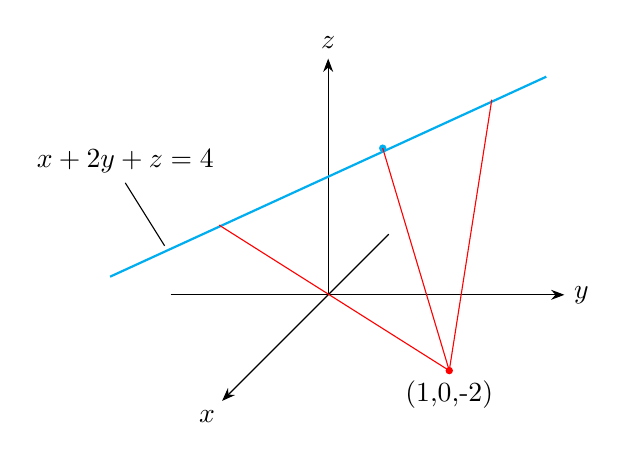
\begin{tikzpicture}[=>stealth]
\draw[-Stealth](-2,0,0)--(3,0,0)node[right]{$y$};
\draw[-Stealth](0,0,0)--(0,3,0)node[above]{$z$};
\draw[-Stealth](0,0,-2)--(0,0,3.5);
\draw(0,0,4)node[]{$x$}
(2.5,0,2.5)node[below]{(1,0,-2)};
\draw[cyan,thick](-2,1,2)--(2,2,-2)
(0.5,1.67,-0.5)node[shape=circle,scale=0.01cm,fill=cyan]{};
\draw[red]
(2.5,0,2.5)node[shape = circle, scale = 0.01cm, fill=red]{}
(2.5,0,2.5)--(-1,1.27,1)
(2.5,0,2.5)--(1.5,1.9,-1.5)
(2.5,0,2.5)--(0.5,1.67,-0.5);
\draw(-2,2,1.5)--(-1.5,1.2,1.5)
(-2,2,1.5)node[above]{$x + 2y + z = 4$};
\end{tikzpicture}
\end{figure}

\vspace{1cm}
\end{solution}

{\color[wave]{485}\subsection{Extrema for Functions with Side Conditions (Constraints)}}

\subhead{Lagrange Multipliers}


Find the extreme values of $f(x,y)$ subject to $g(x,y) =K$. To maximise $f(x,y)$ subject to $g(x,y) = K$ is to find the largest value of $C$ such that the level curve $f(x,y) = C$ intersects the $g(x,y) = K$. This occurs when the curves touch each other i.e when they have a common tangent line.

% DIAGRAM 8 

\begin{figure}[H]
\centering
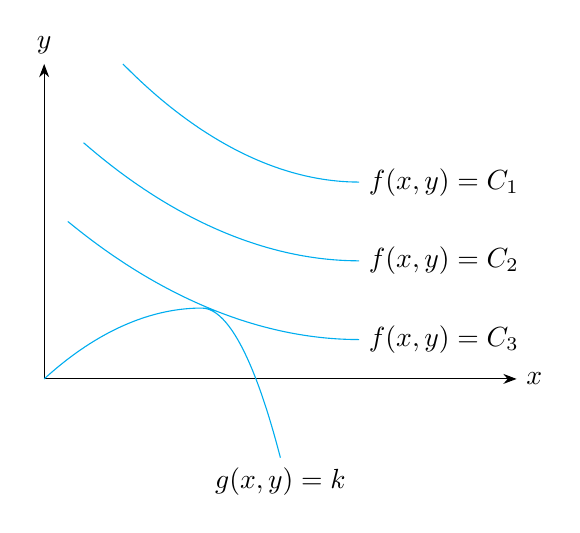
\begin{tikzpicture}[=>stealth]
\draw[-Stealth](0,0)--(6,0)node[right]{$x$};
\draw[-Stealth](0,0)--(0,4)node[above]{$y$};
\draw[cyan](1,4)parabola[bend at end](4,2.5)node[right,black]{$f(x,y)=C_1$}
(0.5,3)parabola[bend at end](4,1.5)node[right,black]{$f(x,y)=C_2$}
(0.3,2)parabola[bend at end](4,0.5)node[right,black]{$f(x,y)=C_3$}
(0,0)parabola[bend at end](2,0.9)
(2,0.9)parabola(3,-1)node[below,black]{$g(x,y)=k$};
\end{tikzpicture}
\end{figure}

This means that the normal lines at the point $(x_0,y_0)$ are identical so the gradient vectors are parallel $$ \nabla f(x,y) = \lambda \nabla g(x,y)$$ for the scalar $\lambda$. The number $\lambda$ is called the Lagrange multiplier.


\subhead{Method of Lagrange Multipliers}


To find the max or min values of $(x,y,z)$ subject to the constraints $g(x,y,z) = K$ (assuming the extreme values exist and $\nabla g(x,y,z) \neq 0)$. on the surface $g(x,y,z) = K$.
\begin{enumerate}
\item Find all the values of $x, y, z$ and $\lambda$ $$\nabla f(x,y,z) = \lambda \nabla g(x,y,z)$$

\item Evaluate $f$ at all points $(x,y,z)$ that result from step (1). The largest value of these gives the maximum value of $f$, and the smallest value gives the minimum value of the function.
\end{enumerate}

\begin{exa}


Find the extreme values of the function $f(x,y) = x + y$ subject to the constraint $x^2 + y^2 = 1$

%DIAGRAM 9 

\begin{figure}[H]
\centering
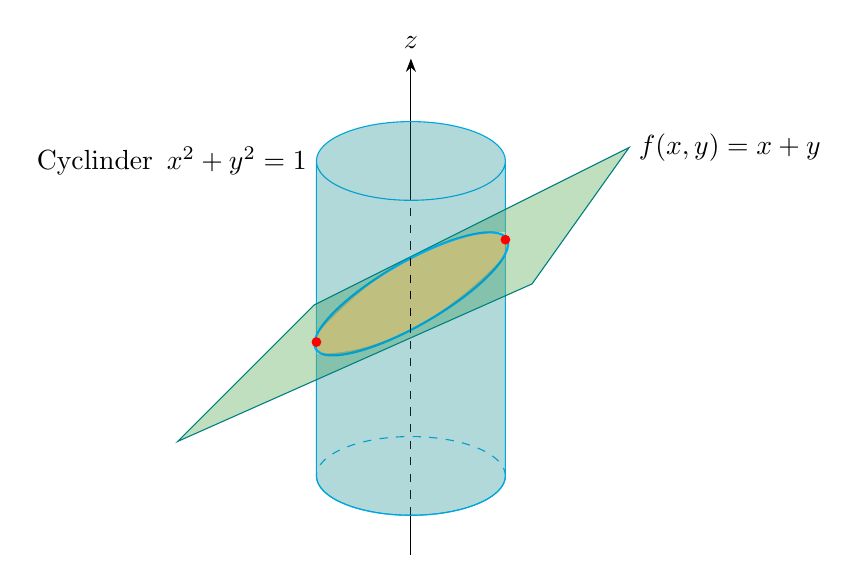
\begin{tikzpicture}[=>stealth]
%\draw[-Stealth](-2,0,0)--(2,0,0)node[right]{$y$};
\draw[-Stealth](0,3.5,0)--(0,5.3,0)node[above]{$z$};
%\draw[-Stealth](0,0,-2)--(0,0,3);
%\draw(0,0,3.5)node[]{$x$};
\draw[cyan](-1.2,0)arc(180:360:1.2cm and 0.5cm)
(1.2,0)--(1.2,4)
(-1.2,0)--(-1.2,4)
(1.2,4)arc(0:360:1.2cm and 0.5cm);
\path[fill=orange,opacity=0.5, rotate=30](2.56,2)arc(0:360:1.4cm and 0.4cm);
\path[fill=orange!50!cyan,opacity=0.5](-2,1.4,2.5)--(2.5,3.4,2.5)--(2,3.4,-2)--(-2,1.4,-2)--cycle;
\draw[teal](-2,1.4,2.5)--(2.5,3.4,2.5)--(2,3.4,-2)--(-2,1.4,-2)--cycle;
%%%
\draw(0,-1)--(0,-0.45)
(2,3.4,-2)node[right]{$f(x,y)=x +y$}
(-1.2,4)node[left]{Cyclinder $\, x^2 + y^2 = 1$};
%\shade[right color=teal,opacity=0.1](1.2,4)arc(0:360:1.2cm and 0.5cm);
\draw[cyan](-1.2,0)arc(180:360:1.2cm and 0.5cm);
\draw[rotate=30,thick,cyan](2.56,2)arc(0:360:1.4cm and 0.4cm);
\draw[dashed,cyan](1.2,0)arc(0:180:1.2cm and 0.5cm);
\draw[dashed](0,-0.5)--(0,3.4);
\draw(1.2,3)node[shape=circle,fill=red,draw=red,thick,scale=0.01cm]{}
(-1.2,1.7)node[shape=circle,fill=red,draw=red,thick,scale=0.01cm]{};
\path[fill=teal,opacity=0.3](-1.2,1.8)--(-1.2,0)--(-1.2,0)arc(180:360:1.2cm and 0.5cm)--(1.2,0)--(1.2,3)--(1.2,2.8)parabola[bend at end](-1.2,1.55)--(-1.2,1.8);
\path[fill=teal,opacity=0.3](1.2,3)--(1.2,4)--(1.2,4)arc(0:180:1.2cm and 0.5cm)--(-1.2,4)--(-1.2,1.8)--(-1.2,1.8)parabola[bend at end](1.2,3.1)--cycle;
\end{tikzpicture}
\end{figure}

$f(x,y) = x + y$


$g(x,y): \hspace{0.3cm} x^2 + y^2 = 1$


$x +  y = z$


$K = x + y$

% DIAGRAM 10

\begin{figure}[H]
\centering
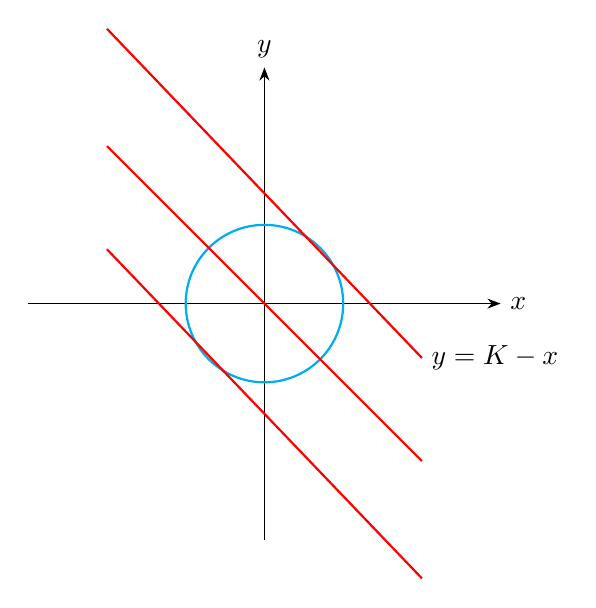
\begin{tikzpicture}[=>stealth]
\draw[-Stealth](-3,0)--(3,0)node[right]{$x$};
\draw[-Stealth](0,-3)--(0,3)node[above]{$y$};
\draw[thick,cyan](0,0)circle [radius=1cm];
\draw[thick,red](-2,2)--(2,-2);
\draw[thick,red](-2,3.49)--(2,-0.69);
\draw[thick,red](-2,0.69)--(2,-3.49);
\draw(2,-0.69)node[right]{$y = K - x$};
\end{tikzpicture}
\end{figure}

\begin{align*}
f(x,y) & = x + y \\
g(x,y) & =x^2 + y^2 - 1
\end{align*}

\begin{align*}
\nabla f & = \lambda \nabla g
\end{align*}

$$\nabla f = \textbf{i} + \,\textbf{j}\hspace{0.2cm},\hspace{0.5cm} \nabla g = 2x\, \textbf{i} + 2y\, \textbf{j}$$

\begin{align*}
1 & = 2x\lambda \hspace{0.5cm}\cdots\cdots\cdots\hspace{0.5cm}  (1)\\
1 & = 2y\lambda \hspace{0.5cm} \cdots\cdots\cdots\hspace{0.5cm} (2)\\\\
1 & = x^2 + y^2\hspace{0.5cm}\cdots\cdots\cdots \hspace{0.5cm}  (3)
\end{align*}

substituting (1) and (2) $\implies x = y$


Stationary $2x^2 = 1 \implies x = \pm \dfrac{\sqrt{2}}{2}$


Stationary points $\bigg(\dfrac{\sqrt{2}}{2}, \dfrac{\sqrt{2}}{2}\bigg)$ and $\bigg(-\dfrac{\sqrt{2}}{2}, -\dfrac{\sqrt{2}}{2}\bigg)$.


$f\bigg(\dfrac{\sqrt{2}}{2}, \dfrac{\sqrt{2}}{2}\bigg)=\sqrt{2}\hspace{1cm}$ Max


$f\bigg(\dfrac{-\sqrt{2}}{2}, \dfrac{-\sqrt{2}}{2}\bigg)=-\sqrt{2}\hspace{1cm}$ Min

% DIAGRAM 11

\begin{figure}[H]
\centering
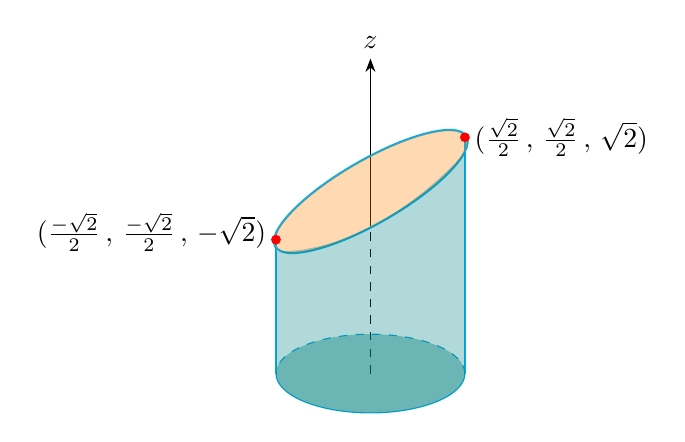
\begin{tikzpicture}[=>stealth]
%\draw[-Stealth](1.2,0,0)--(2.3,0,0)node[right]{$y$};
\draw[-Stealth](0,1.87,0)--(0,4,0)node[above]{$z$};
%\draw[-Stealth](0,0,1.2)--(0,0,3);
\draw[cyan](-1.2,0)arc(180:360:1.2cm and 0.5cm);
\draw[cyan](1.2,0)--(1.2,3)
(-1.2,0)--(-1.2,1.8);
\draw[rotate=30,thick,cyan](2.56,2)arc(0:360:1.4cm and 0.4cm);
\path[fill=orange,opacity=0.3, rotate=30](2.56,2)arc(0:360:1.4cm and 0.4cm);
\draw[dashed,cyan](1.2,0)arc(0:180:1.2cm and 0.5cm);
\draw[dashed](0,0)--(0,1.8);
\draw(1.2,3)node[shape=circle,fill=red,draw=red,thick,scale=0.01cm]{}
(-1.2,1.7)node[shape=circle,fill=red,draw=red,thick,scale=0.01cm]{}
(1.2,3)node[right]{$(\frac{\sqrt{2}}{2}\, ,\, \frac{\sqrt{2}}{2}\, ,\, \sqrt{2})$}
(-1.2,1.8)node[left]{$(\frac{- \sqrt{2}}{2}\, ,\, \frac{-\sqrt{2}}{2}\, ,\, -\sqrt{2})$};
\path[fill=teal,opacity=0.4](1.2,0)arc(0:360:1.2cm and 0.5cm);
\path[fill=teal,opacity=0.3](-1.2,1.8)--(-1.2,0)--(-1.2,0)arc(180:360:1.2cm and 0.5cm)--(1.2,0)--(1.2,3)--(1.2,2.8)parabola[bend at end](-1.2,1.55)--(-1.2,1.8);
\end{tikzpicture}
\end{figure}
\end{exa}

\begin{exa}


Find the extreme values of the function $f(x,y) = x^2 + 2y^2$ on the circle $x^2 + y^2 = 1$


\begin{align*}
\nabla f & = \lambda \nabla g\\\\
\nabla f & = 2x\,\textbf{i}+ 4y\,\textbf{j}\\
\nabla g & = 2x\,\textbf{i} + 2y\,\textbf{j}
\end{align*}

\begin{align*}
2x & = 2x\lambda\\
4y & = 2y\lambda
\end{align*}

$2x = 2x\lambda \implies x = 0$ or $\lambda = 1$


If $\lambda = 1$, then $y = 0$
\begin{align*}
x^2 + y^2  = 1 \implies & x = 0, \hspace{0.3cm} y \neq 1\\
                        & y = 0 , \hspace{0.3cm} y \neq \pm 1
\end{align*}

Therefore, $f$ has possible extreme values at the points $(0,-1), (0,1)$ or $(1,0), (-1,0)$

\begin{align*}
f(x,y)  & = x^2 + y^2\\\\
f(1,0) & =1 \hspace{0.4cm},\hspace{0.4cm} f(0,1) = 2\\
f(-1,0) & =1 \hspace{0.4cm},\hspace{0.4cm} f(0,-1) = 2
\end{align*}

The max value of $f$ on the circle $x^2 + y^2 = 1$ is $f(0,\pm 1)= 2$ and the min is $f(\pm, 0)=1$

% DIAGRAM 12

\begin{figure}[H]
\centering
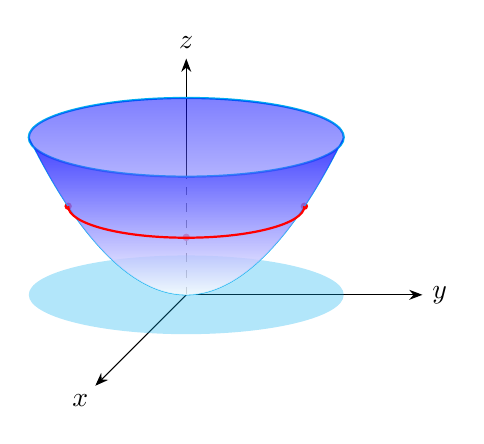
\begin{tikzpicture}[=>stealth]
\draw[-Stealth](0,0,0)--(3,0,0)node[right]{$y$};
\draw[-Stealth](0,1.5,0)--(0,3,0)node[above]{$z$};
\draw[-Stealth](0,0,0)--(0,0,3);
\draw[dashed](0,0,0)--(0,1.5,0);
\draw(0,0,3.5)node[]{$x$}
(-1.5,1.125)node[shape=circle,fill=red,scale=0.01cm]{}
(0,0.73)node[shape=circle,fill=red,scale=0.01cm]{}
(1.5,1.125)node[shape=circle,fill=red,scale=0.01cm]{};
\path[fill=cyan,opacity=0.3](0,0)circle(2cm and 0.5cm);
\draw[cyan](0,0) parabola(2,2)
(0,0)parabola(-2,2);
\draw[thick,cyan](0,2)ellipse[x radius = 2cm , y radius = 0.5cm];
\shade[top color=blue,opacity=0.5](0,0)parabola(-2,2)--(-2,2)arc(180:0:2cm and 0.5cm)--(2,2)parabola[bend at end](0,0);
\shade[top color=blue,opacity=0.6](0,0)parabola(-2,2)--(-2,2)arc(180:360:2cm and 0.5cm)--(2,2)parabola[bend at end](0,0)--cycle;
\draw[thick,red](-1.5,1.125)arc(180:360:1.5cm and 0.4cm);
\end{tikzpicture}
\end{figure}
\end{exa}

\subhead{Two Constraints}


Let $f(x,y,z)$ be a function to be minimised/maximised subject to two constraints
\begin{align*}
g(x,y,z) & =0\\
h(x,y,z) & =0
\end{align*}
$$\nabla f(x,y,z) =\lambda \nabla g(x,y,z) + \mu \nabla h(x,y,z)$$

$f_x = \lambda g_x + \mu h_x$


$f_y = \lambda g_y + \mu h_y$


$f_z = \lambda g_z + \mu h_z$

\begin{align*}
g(x,y,z) & = K\\
h(x,y,z) & = C\\\\
\end{align*}

\begin{exa}


Find the maximum value of the function $f(x,y,z) = x + 2y + 3z$ on the curve of intersection of the place $x - y - z =1$ and the cylinder $x^2 + y^2 = 1$.
\end{exa}


\begin{solution}


$\nabla f = \textbf{i} + 2\,\textbf{j} + 3\,\textbf{k}$


$\nabla g = \textbf{i} - \textbf{j} - \textbf{k}$


$\nabla h = 2x\,\textbf{i} + 2y\,\textbf{j}$

\begin{align*}
\implies \hspace{1cm} 1 & = \lambda + 2x\mu \hspace{1.4cm} (1)\\
                      2 & = -\lambda + 2y\mu \hspace{1cm} (2)\\
                      3 & = \lambda \hspace{2.5cm} (3)\\\\
         x - y + z & = 1 \hspace{2.5cm} (4)\\
         x^2 + y^2 & = 1\hspace{2.5cm} (5)\\
\end{align*}

Taking $\lambda = 3$, substituting into (1) and (2) we have
\begin{align*}
2x\mu & = -2 \implies x = \frac{-1}{\mu}\\\\
2y\mu & = 5 \implies y = \frac{5}{2\mu}
\end{align*}
substituting these into (5)
$$\frac{1}{\mu^2}+ \frac{25}{4\mu^2} = 1 \implies \mu^2 = \frac{29}{4}\implies \mu = \pm\frac{\sqrt{29}}{2}$$


$$x = \pm \frac{2}{\sqrt{29}}\hspace{0.5cm},\hspace{0.5cm} y = \pm \frac{5}{\sqrt{29}}$$


\begin{align*}
z & = 1 -x - y\\\\
 & = 1 - \bigg(\pm\frac{2}{\sqrt{29}}\bigg) + \bigg(\pm \frac{5}{\sqrt{29}}\bigg)\\\\
\implies \hspace{1cm} z & = 1 \pm \frac{7}{\sqrt{29}}\\
\end{align*}

\begin{align*}
f(x,y,z) & = x + 2y + 3z\\\\
& = \bigg(\pm \frac{2}{\sqrt{29}}\bigg) + 2\bigg(\pm \frac{5}{\sqrt{29}}\bigg) + 3\bigg( 1 \pm \frac{7}{\sqrt{29}}\bigg)\\
\end{align*}

Critical points $\bigg(\dfrac{2}{\sqrt{29}}, \dfrac{-5}{\sqrt{29}}, 1 - \dfrac{7}{\sqrt{29}}\bigg)$ and $\bigg(\dfrac{-2}{\sqrt{29}}, \dfrac{5}{\sqrt{29}}, 1 + \dfrac{7}{\sqrt{29}}\bigg)$.


Max value is $3 + \sqrt{29}$
\end{solution}


{\color[wave]{485}\subsection{Absolute Maximum and Minimum Values}}
Extreme value theorem for functions of two variables.


If $f$ is continuous on a closed bounded set in $D$ in $\mathbb{R}^2$, then $f$ attains an absolute maximum value $f(x_1,y_1)$ and absolute minimum value at $f(x_2,y_2)$ at some points in $D$.


\subhead{Closed Interval Method}
\begin{enumerate}
\item Find the values of  $f$ at the critical point of $f$ in $D$.

\item Find the extreme points on the boundary.

\item Largest of the values of $f$ from steps 1 and 2 is the absolute maximum value and the smallest of the values is the absolute minimum.
\end{enumerate}

\begin{exa}


Find the absolute max and min values of the function $f(x,y) = x^2 - 2xy + 2y$ of the  rectangle $D = \big\{(x,y)\hspace{0.1cm} \big| \hspace{0.1cm} 0\leq x \leq 3\hspace{0.1cm} , \hspace{0.1cm} 0 \leq y \leq 2 \big\}$.
\end{exa}


\begin{solution}


$f$ is continuous on $D$


$f_x = 2x -2y = 0 \implies x = y$


$f_y = -2x + 2 = 0 \implies x = 1$


$(1,1)$ is the only critical point and $f(1,1) = 1$.

% DIAGRAM 13

\begin{figure}[H]
\centering
\begin{tikzpicture}[=>stealth]
\draw[-Stealth](0,0)--(4,0)node[right]{$x$};
\draw[-Stealth](0,0)--(0,3)node[above]{$y$};
\draw[cyan](0,0)rectangle(3,2);
\draw(0,0)node[below]{$0$}
(3,0)node[below]{$3$}
(3,2)node[right]{$(3,2)$}
(0,2)node[left]{$2$}
(1.5,0)node[below,scale=0.9]{$L_1$}
(3,1)node[right,scale=0.9]{$L_2$}
(1.5,2)node[above,scale=0.9]{$L_3$}
(0,1)node[left,scale=0.9]{$L_4$};
\end{tikzpicture}
\end{figure}
\end{solution}

{\color[wave]{485}\subsection{Taylor's Formula For Functions of Several Variables}}

Recall: $n^{\text{th}}$ degree Taylor polynomial $$f(x) \approx f(a) + \frac{f'(a)(x-a)}{1!}+ \frac{f''(a)(x-a)^2}{2!}+ \frac{f'''(a)(x-a)^3}{3!}+ \cdots\cdots\cdots\cdots + \frac{f^n(a)(x-a)^n}{n!}$$


Two variables
$$F(x,y) = F(x_1,y_1) + dF(x_1,y_1,x-x_1,y-y_1) + \frac{d^n}{n!}F(x_1,y_1,x-x_1,y-y_1)$$

For $n = 1$
$$F(x,y) = F(x_1,y_1) + dF(x_1,y_1,x-x_1,y-y_1)$$

This is known as the mean value theorem.


If $f(x,y)$ and its partial derivatives upto the $n^{\text{th}}$ order are finite and continuous for all points $(x,y)$ where $a\leq x\leq  a+h\hspace{0.2cm},\hspace{0.2cm} b\leq y \leq b + k$. Then 

$$f(a+h,b+k) = f(a,b) + \bigg(h\frac{\partial}{\partial x} + k \frac{\partial}{\partial y}\bigg) f + \frac{\bigg(h\dfrac{\partial}{\partial x} + k \dfrac{\partial}{\partial y}\bigg)^2f}{2!} + \frac{\bigg(h\dfrac{\partial}{\partial x} + k \dfrac{\partial}{\partial y}\bigg)^3 f}{3!} + \cdots\cdots\cdots 
$$

Let $a=0,\hspace{0.3cm} b = 0,\hspace{0.3cm} h=x,\hspace{0.3cm} k = y$

\begin{align*}
f(x,y) = & f(0,0) + \frac{1}{1!}\bigg(x\frac{\partial f}{\partial x} + y \frac{\partial f}{\partial y}\bigg) 
+\frac{1}{2!}\bigg(x^2\frac{\partial^2 f}{\partial x^2} + y^2\frac{\partial^2f}{\partial y^2} +2xy\frac{\partial^2f}{\partial x\partial y}\bigg)\\\\ & + \frac{1}{3!}      
\bigg(x^3\frac{\partial^3f}{\partial x^3} + 3x^2y \frac{\partial^3f}{\partial x^2\partial y} + 3xy^2\frac{\partial^3f}{\partial x\partial y^2} + y^3 \frac{\partial^3f}{\partial y^3}\bigg) +\cdots\cdots\cdots\cdots\\
\end{align*}

\begin{exa}


Expand $f(x,y) = e^x \sin y$ about $(0,0)$ in powers of $x$ and $y$ upto terms of third degree.
\end{exa}


\begin{solution}


$f(x,y) = e^x\sin y$


$f_x = e^x\sin y\hspace{1cm} f_x(0,0) = 0$


$f_y = e^x \sin y\hspace{1cm} f_y(0,0) = 1$


$f_{xx} = e^x\sin y \hspace{1cm} f_{xx} (0,0) = 0$


$f_{xy} = e^x \cos y \hspace{1cm} f_{xy} (0,0) = 1$


$f_{yy} = -e^x \sin y \hspace{1cm} f_{yy} (0,0) = 0$


$f_{xxx} = e^x \sin y \hspace{1cm} f_{xxx} (0,0) = 0$


$f_{xxy} = e^x\cos y \hspace{1cm} f_{xxy} (0,0) = 1$


$f_{xyy} = -e^x\sin y \hspace{1cm} f_{xyy} (0,0) = 0$


$f_{yyy} = -e^x \cos y \hspace{1cm} f_{yyy} (0,0) = -1$


By Taylor's theorem
\begin{align*}
f(x,y)  = & f(0,0) + xf_x(0,0) + yf_y(0,0) + \frac{1}{2!}\bigg(x^2f_{xx}(0,0) + 2xyf_{xy}(0,0) +y^2f_{yy}(0,0)\bigg)\\ + &\frac{1}{3!}\bigg(x^3f_{xxx}(0,0) + 3x^2yf_{xxy}(0,0) + 3xy^2f_{xyy}(0,0) + y^3f_{yyy}(0,0)\bigg) + \cdots\cdots\cdots\\
\end{align*}

$$\implies\hspace{1cm} f(x,y) = y + xy + \frac{x^2y}{2} - \frac{y^3}{6} + \cdots\cdots\cdots\cdots$$
\end{solution}


\begin{exa}


Expand $x^2y + 3y -2$ in powers of $x - 1$ and $y + 2$.
\end{exa}


\begin{solution}


$f(x,y) = x^2y + 3y -2$


$f_x = 2xy\hspace{1cm} f_x(1,-2) = -4$


$f_y = x^2 + 3\hspace{1cm} f_y (1,-2) = 4$


$f_{xx} = 2y \hspace{1cm} f_{xx}(1,-2) = -4$


$f_{yy} = 0 \hspace{1cm}  f_{yy} (1,-2) = 0$


$f_{xy} = 2x\hspace{1cm} f_{xy} (1,-2) = -4$


$f_{xxx} = 0$


$f_{xxy} = 2$


$f_{xyy} = 0$


$f_{yyy} = 0$


\begin{align*}
f(x,y) = & f(1,-2) + (x-1)f_x(1,-2) + (y+2)f_y(1,-2)\\ & + \frac{1}{2!}\big[(x-1)^2 f_{xx}(1,-2) + 2(x-1)(y+2)f_{xy}f(1,-2) + (y+2)^2f_{yy}(1,-2)\big]\\
 & + \frac{1}{3!}\big[3(x-1)^2(y+1)f_{xxy}(1,-2)\big]
\end{align*}

\begin{align*}
f(x,y) = & -10 - 4(x-1) + 4(y+2) + \frac{1}{2!}\big(-4(x-1)^2 +4(x - 1) (y+2)\big) + \frac{1}{3!}\big(6(x-1)^2(y+2)\big)\\\\
\end{align*}
\end{solution}

\begin{exe}


Find the expansion for $\cos x \cos y$ in powers of $x$ and $y$ upto the fourth order terms.

$$\textbf{Ans:}\hspace{1cm} f(x,y) = 1 - \frac{x^2}{2}-\frac{y^2}{2} + \frac{x^4}{24} + \frac{x^2y^2}{4} + \frac{y^4}{24}+\cdots\cdots\cdots\cdots$$


\pagebreak
\end{exe}
{\color[wave]{485}\subsection{Composite Functions and Chain Rule Differentiation}}
Let $z = f(x,y)$ where $x = g(r,s)$ and $y = (r,s)$ , so that $z$ is a function of $r$ and $s$. Then $$\frac{\partial z}{\partial r} =\frac{\partial z}{\partial x}\cdot \frac{\partial x}{\partial r} + \frac{\partial z}{\partial y}\cdot \frac{\partial y}{\partial r}$$ 

In general if $u  = F(x_1,x_2,\cdots\cdots\cdots, x_n)$ where $x_1 = f_1 (r_1,r_2,\cdots\cdots\cdots, r_n)$ then $$\frac{\partial u}{\partial r_1}=\frac{\partial u}{\partial x_1}\frac{\partial x_1}{\partial r_1}+ \frac{\partial u}{\partial x_2} \cdot \frac{\partial x_2}{\partial r_1}+\cdots\cdots\cdots + \frac{\partial u}{\partial x_n}\cdot \frac{\partial x_n}{\partial r_1}$$

In particular if $x_1,x_2,\cdots\cdots\cdots, x_n$ depend only on one variable ,$s$, then 
 $$\frac{du}{ds} = \frac{\partial u}{\partial x_1}\cdot \frac{dx_1}{ds}+ \frac{\partial u}{\partial x_2}\cdot \frac{dx_2}{ds} +\cdots\cdots\cdots +\frac{\partial u}{\partial x_n}\cdot \frac{dx_n}{ds}$$

These results are called chain rule and are useful in transforming derivatives from one set of variables to another.


\begin{exa}


If $f(x) = \sin x\hspace{0.4cm}, \hspace{0.4cm} x = t^2\hspace{1cm} -\infty < t < \infty$


Then $\hspace{0.4cm} f(x(t)) = \sin (t^2) = F(t)$
\begin{align*}
\frac{dF}{d t} &  = \frac{d F}{dx}\cdot \frac{d x}{dt}\\
& = \cos x \cdot 2t\\
& = 2t\cos(t^2)\\
\end{align*}
\end{exa}

\begin{exa}


Let $r(x,y) =x^2y - e^{2y}$


where$\hspace{0.4cm} x = 3t^2\hspace{1cm} y = \sin t \hspace{1cm}  1< t <4$


Then $\hspace{0.5cm} r\big(x(t),y(t)\big) =  \hspace{0.5cm} = R(t)$

\begin{align*}
\frac{dR}{dt} & = \frac{\partial R}{\partial x}\cdot \frac{dx}{dt} + \frac{\partial R}{\partial y}\cdot \frac{dy}{dt}\\
&  = 2xy\cdot 6t + \big(x^2 - 2e^{2y}\big)\cdot \cos t\\
& = 2\cdot 3t^2\cdot \sin t \cdot 6t + \big(\big(3t^2\big)^2 - 2e^{2\sin t}\big) \cdot \cos t\\
& = 36t^3\sin t + \big( 9t^4 - 2e^{2\sin t}\big)\cos t\\ 
\end{align*}
\end{exa}

\begin{exa}


Let $f(u,v) = uv^2$


where $\hspace{0.5cm} u = 3x-y\hspace{0.5cm}, \hspace{0.5cm} v = x^2y$

$$f(u,v) = f\big(u(x,y), v(x,y)\big) = F(x,y)$$

\begin{align*}
\frac{\partial F}{\partial x} & = \frac{\partial F}{\partial u}\cdot \frac{\partial u}{\partial x} + \frac{\partial F}{\partial v}\cdot \frac{\partial v}{\partial x}\\
& = v^2(3) + 2uv(2xy)\\
& = 3x^4y^2 + 2(x^2y)(3x - y) \cdot 2xy\\
& = 15x^4y^2 - 4x^3y^3\\ 
\end{align*}

\begin{align*}
||||_y\hspace{1cm}  \frac{\partial F}{\partial y} & = \frac{\partial F}{\partial u}\cdot \frac{\partial u}{\partial y} +\frac{\partial F}{\partial v}\cdot \frac{\partial v}{\partial y}\\
& = v^2(-1) + 2uv\cdot x^2\\
& = -\big(x^2y\big)^2 + 2\big(3x -y\big)\big(x^2y\big)\cdot x^2\\
& = -x^4y^2 + \big(6x -2y\big)x^4y\\
& = 6x^5y - 3x^4y^2\\ 
\end{align*}
\end{exa}

{\color[wave]{485}\subsection{Euler's Theorem on Homogeneous Functions}}
A function $F(x_1,x_2,\cdots\cdots\cdots, x_n)$ is called homogeneous of degree $P$ if for all values of the parameter $\lambda$ and same constant $P$ we have the identity
$$F(\lambda x_1,\lambda x_2,\cdots\cdots\cdots, \lambda x_n) = \lambda^P F(x_1,x_2,\cdots\cdots\cdots,x_n)$$


\begin{exa}


$F(x,y) = x^4 + 2xy^3 - 5y^4$
\begin{align*}
F\big(\lambda x, \lambda y\big) & = \big(\lambda x\big)^4 + 2\big(\lambda x\big)\big(\lambda y\big)^3 - 5\big(\lambda y\big)^4\\
& = \lambda^4 x^4 + 2\lambda^4xy^3 - 5\lambda^4 y^4\\
& = \lambda^4 \big(x^4 +2xy^3 - 5y^4\big)
\end{align*}
$\therefore\hspace{0.4cm}F(x,y)$ is a homogeneous of degree 4.


Euler's theorem on homogeneous functions states that if $F(x_1,x_2,\cdots\cdots\cdots, x_n)$ is homogeneous of degree $P$ then 
$$ x_1 \frac{\partial F}{\partial x_1} + x_2 \frac{\partial F}{\partial x_2} + \cdot\cdots\cdots +x_n \frac{\partial F}{\partial x_n} = P F$$

In the previous example
\begin{align*}
x \frac{\partial F}{\partial x} + y \frac{\partial F}{\partial y} & = 4 F\\
x\big(4x^3 + 2y^3\big) + y\big(6xy^2 -20y^3\big) &  = 4 \big( x^4 + 2xy^3 - 5y^4\big)\\\\\\\
\end{align*}
\end{exa}

{\color[wave]{485}\subsection{Implicit Functions and Jacobians}}
If $F(x,y,z) =0$ is a given function of $x,y,z$  then the equation $$F(x,y,z) =0$$ is a relation that may describe one or more several functions $z$ of $x$ and $y$
$$\text{e.g}\hspace{0.2cm} x^2 + y^2+ z^2 - 1 = 0$$

$$F(x,y,z) = 0$$

But $z = \pm \sqrt{1 -x^2 -y^2}$ , both functions being defined on $x^2  + y^2 \leq 1$.


Either function is said to be implicitly defined by $$x^2 + y^2 + z^2 - 1 =0$$ as distinguished from a so - called explicit function of $f$ where $z = f(x,y)$, such that $F(x,y,f(x,y))$.


Similarly, an equation $F(x,y,z,w)=0$ may define one or more implicit functions of $x,y,z$.


\begin{exa}


Consider the relation $$x^2 + 4y^2 - 4 =0\hspace{0.5cm}\cdots\cdots\cdots\hspace{0.5cm} (1)$$ satisfied by the points on an ellipse shown below.

% DIAGRAM 14

\begin{figure}[H]
\centering
\begin{tikzpicture}[=>stealth]
\draw[-Stealth](-3,0)--(3,0)node[right]{$x$};
\draw[-Stealth](0,-2)--(0,2)node[above]{$y$};
\draw[thick,cyan](0,0)ellipse[x radius = 2cm, y radius = 1cm];
\draw(1.3,0.77)node[shape=circle,thick,draw=cyan,fill=cyan,scale=0.01cm]{}
(1.3,-0.77)node[shape=circle,thick,draw=cyan,fill=cyan,scale=0.01cm]{}
(0,1)node[shape=circle,thick,draw=cyan,fill=cyan,scale=0.01cm]{}
(0,-1)node[shape=circle,thick,draw=cyan,fill=cyan,scale=0.01cm]{}
(1.3,0.77)node[above]{$b$}
(1.3,-0.77)node[below]{$d$}
(-0.1,1.2)node[left]{$a$}
(-0.1,-1.2)node[left]{$c$};
\end{tikzpicture}
\end{figure}

Clearly equation (1) is an implicit function, $y(x)$ and $\displaystyle{y = \pm \sqrt{1 - \bigg(\dfrac{x}{2}\bigg)^2}}$ with two solutions in the interval $0< x<1$.


In some cases, we may not be able to solve for $y(x)$.


e.g $2xy + \sin y =0$ is a transcendental equation.
\end{exa}


\subhead{The General Chain Rule}


Suppose that you have two sets of functions 
\begin{align*}
y_1 & = f_1 (u_1,u_2,\cdots\cdots\cdots, u_p)\\
\vdots &\\
        &   \hspace{6cm} (1)\\
\vdots &\\
y_n & = f_n (u_1,u_2,\cdots\cdots\cdots, u_p)
\end{align*}

and

\begin{align*}
u_1 & = g_1 (x_1,x_2,\cdots\cdots\cdots, x_n)\\
\vdots &\\
        &   \hspace{6cm} (2)\\
\vdots &\\
u_p & = g_p (x_1,x_2,\cdots\cdots\cdots, x_n)
\end{align*}

substituting (2) in (1)

\begin{align*}
y_1 & = f_1\big( g_1(x_1,x_2,\cdots\cdots\cdots, x_m) \cdots\cdots g_p (x_1,x_2,\cdots\cdots\cdots, x_m)\big)\\
\vdots & \\
\vdots & \\
y_n & = f_n \big(g_1(x_1,x_2,\cdots\cdots\cdots, x_m)\cdots\cdots g_p (x_1,x_2,\cdots\cdots\cdots, x_m)\big)
\end{align*}

one can obtain partial derivatives of these composite functions
$$\frac{\partial y_i}{\partial x_j} = \frac{\partial y_i}{\partial u_1}\cdot \frac{\partial u_1}{\partial x_j} + \frac{\partial y_i}{\partial u_2}\cdot\frac{\partial u_2}{\partial x_j} + \cdots\cdots\cdots + \frac{\partial y_i}{\partial u_p}\cdot\frac{\partial u_p}{\partial x_j}$$ $$\hspace{0.5cm} i = 1,2,\cdots\cdots, n\hspace{0.4cm} j = 1,2,\cdots\cdots, m$$

This can be expressed concisely in matrix language.

$$\frac{\partial y_i}{\partial x_j}=
\begin{bmatrix}
\dfrac{\partial y_1}{\partial x_1} & \dfrac{\partial y_1}{\partial x_2} & \cdots\cdots & \dfrac{\partial y_1}{\partial x_m}\\\\
\vdots & && \vdots\\\\
\dfrac{\partial y_n}{\partial x_1} & \dfrac{\partial y_n}{\partial x_2} & \cdots\cdots & \dfrac{\partial y_n}{\partial x_m}
\end{bmatrix}
$$

This is the Jacobian matrix of mapping (1).


The formula involve two other Jacobian matrices

$$ \frac{\partial y_i}{\partial u_j}=
\begin{bmatrix}
\dfrac{\partial y_1}{\partial u_1} & \cdots\cdots\cdots & \dfrac{\partial y_1}{\partial u_p}\\\\
\vdots &&\vdots\\\\
\dfrac{\partial y_n}{\partial u_1} & \cdots\cdots\cdots & \dfrac{\partial y_n}{\partial u_p}\\
\end{bmatrix}
$$


$$\Bigg(\frac{\partial u_i}{\partial x_j}\Bigg) =
\begin{bmatrix}
\dfrac{\partial u_1}{\partial x_1} & \cdots\cdots\cdots & \dfrac{\partial u_1}{\partial x_m}\\\\
\vdots &&\vdots\\\\
\dfrac{\partial u_p}{\partial x_1} & \cdots\cdots\cdots & \dfrac{\partial u_p}{\partial x_m}\\
\end{bmatrix}
$$

The last two expressions (Jacobians Matrices) equal the previous one
$$\frac{\partial y_i}{\partial x_j}= \Bigg(\frac{\partial y_i}{\partial u_j}\Bigg)\Bigg(\frac{\partial u_j}{\partial x_j}\Bigg)$$
is called the general chain rule.


\begin{exa}


The mapping $\hspace{0.2cm} x = \cos u \cos v,\hspace{0.5cm} y = \cos u \sin v,\hspace{0.5cm} z = \sin u$ is given.\\ Find the Jacobian matrix.

$$
\begin{bmatrix}
\dfrac{\partial x}{\partial u} & \dfrac{\partial x}{\partial v}\\\\
\dfrac{\partial y}{\partial u} & \dfrac{\partial y}{\partial v}\\\\
\dfrac{\partial z}{\partial u} & \dfrac{\partial z}{\partial v}\\
\end{bmatrix} =
\begin{bmatrix}
-\sin u \cos v & - \cos u\sin v\\
-\sin u \sin v & \cos u \cos v\\
\cos u         & 0\\
\end{bmatrix}
$$
$\implies$ is the Jacobian matrix for the given mapping.


Assuming $m=n$, the Jacobian matrix will be a square matrix and we can find its determinant
$$ J = \det \Bigg(\frac{\partial y_i}{\partial x_j}\Bigg)=
\begin{vmatrix}
\dfrac{\partial y_1}{\partial x_1} & \dfrac{\partial y_1}{\partial x_2} & \cdots\cdots & \dfrac{\partial y_1}{\partial x_m}\\\\
\vdots & && \vdots\\\\
\dfrac{\partial y_n}{\partial x_1} & \dfrac{\partial y_n}{\partial x_2} & \cdots\cdots & \dfrac{\partial y_n}{\partial x_m}
\end{vmatrix}
$$
called the Jacobian determinant.


Also
$$J = \frac{\partial(y_1,\cdots\cdots\cdots,y_n)}{\partial (x_1,\cdots\cdots\cdots,x_m)} = \frac{\partial (f_1,\cdots\cdots\cdots,f_n)}{\partial (x_1,\cdots\cdots\cdots,x_n)}$$
\end{exa}


{\color[wave]{485}\subsection{Jacobians}}
If $F(u,v)$ and $G(u,v)$ are differentiable in a region, then Jacobian determinant (or Jacobian) of $F$ and $G$ with respect to $u$ and $v$ is the second order functional determinant defined by 
$$ \frac{\partial \big(F,G\big)}{\partial\big(u,v\big)} =
\begin{vmatrix}
\dfrac{\partial F}{\partial u} & \dfrac{\partial F}{\partial v}\\\\
\dfrac{\partial G}{\partial u} & \dfrac{\partial G}{\partial v}\\
\end{vmatrix}
$$

$|||_y$, the third order determinant
$$  \frac{\partial \big(F,G, H\big)}{\partial\big(u,v,w\big)} =
\begin{vmatrix}
\dfrac{\partial F}{\partial u} & \dfrac{\partial F}{\partial v} &  \dfrac{\partial F}{\partial w}\\\\
\dfrac{\partial G}{\partial u} & \dfrac{\partial G}{\partial v} &  \dfrac{\partial G}{\partial w}\\\\
\dfrac{\partial H}{\partial u} & \dfrac{\partial H}{\partial v} &  \dfrac{\partial H}{\partial w}\\
\end{vmatrix}
$$
is called the determinant of $F$, $G$, $H$ with respect to $u,v,w$.


\subhead{Properties of Jacobians}
\begin{enumerate}
\item If $u$ and $v$ are functions of $x$ and $y$ then $$\frac{\partial \big(u,v\big)}{\partial\big(x,y\big)}\times \frac{\partial \big(x,y\big)}{\partial\big(u,v\big)}=1$$
\item If $x$ and $y$ are functions of $u$ and $v$ while $u$ and $v$ are functions of $r$ and $s$, then $$\frac{\partial \big(x,y\big)}{\partial\big(r,s\big)} = \frac{\partial \big(x,y\big)}{\partial \big(u,v\big)}\times \frac{\partial\big(u,v\big)}{\partial \big(r,s\big)}\hspace{0.3cm}\text{Chain Rule}$$
\end{enumerate}

\begin{exa}
If $x = uv$ and $y =\dfrac{u + v}{u -v}$ find $$\frac{\partial \big(u,v\big)}{\partial\big(x,y\big)}=
\begin{vmatrix}
\dfrac{\partial u}{\partial x} & \dfrac{\partial u}{\partial y}\\\\
\dfrac{\partial v}{\partial x} & \dfrac{\partial v}{\partial y}\\
\end{vmatrix}
$$
\end{exa}

\begin{solution}
but $\dfrac{\partial u}{\partial x}, \dfrac{\partial u}{\partial y}, \dfrac{\partial v}{\partial x}$ and $\dfrac{\partial v}{\partial y}$ are comparatively difficult  than $\dfrac{\partial x}{\partial u}, \dfrac{\partial x}{\partial v}, \dfrac{\partial y}{\partial u}$ and $\dfrac{\partial y}{\partial v}$.

 So we find $\frac{\partial \big(x,y\big)}{\partial\big(u,v\big)}$.
\begin{align*}
\frac{\partial \big(x,y\big)}{\partial\big(u,v\big)} & =\begin{vmatrix}
\dfrac{\partial x}{\partial u} & \dfrac{\partial x}{\partial v}\\\\
\dfrac{\partial y}{\partial u} & \dfrac{\partial y}{\partial v}\\
\end{vmatrix}=
\begin{vmatrix}
v & u\\\\
\dfrac{-2v}{(u-v)^2} & \dfrac{2u}{(u-v)^2}\\
\end{vmatrix}\\\\
& = \frac{4uv}{(u -v)^2}
\end{align*}
but\hspace{0.5cm}$\dfrac{\partial \big(u,v\big)}{\partial\big(x,y\big)}\times \dfrac{\partial \big(x,y\big)}{\partial\big(u,v\big)}=1$
$$\therefore\hspace{0.5cm}\frac{\partial \big(u,v\big)}{\partial\big(x,y\big)} = \frac{(u -v)^2}{4uv}$$
\end{solution}

\begin{exe}
If $xyz =h,\hspace{0.3cm} v = x^2 + y^2 + z^2,\hspace{0.3cm} w = x+y+z,$ find $\dfrac{\partial \big(x,y,z\big)}{\partial\big(h,v,w\big)}$
\end{exe}

\begin{exa}
Find the Jacobian $\dfrac{\partial \big(u,v\big)}{\partial \big(r,\theta\big)}$ where $u = x^2 - y^2,\hspace{0.3cm} v = 2xy$ and $x = r\cos \theta,\hspace{0.3cm} y = r\sin \theta$.
\end{exa}

\begin{solution}
\begin{align*}
\frac{\partial \big(u,v\big)}{\partial\big(r,\theta\big)} & = \frac{\partial \big(u,v\big)}{\partial \big(x,y\big)}\times \frac{\partial\big(x,y\big)}{\partial \big(r,\theta\big)}\\\\
& = \begin{vmatrix}
\dfrac{\partial u}{\partial x} & \dfrac{\partial u}{\partial y}\\\\
\dfrac{\partial v}{\partial x} & \dfrac{\partial v}{\partial y}\\
\end{vmatrix} \times
\begin{vmatrix}
\dfrac{\partial x}{\partial r} & \dfrac{\partial x}{\partial \theta}\\\\
\dfrac{\partial y}{\partial r} & \dfrac{\partial y}{\partial \theta}\\
\end{vmatrix}\\\\
& = \begin{vmatrix}
2x & -2y\\
2y & 2x\\
\end{vmatrix}\times 
\begin{vmatrix}
\cos \theta & -r\sin \theta \\
\sin \theta & r\cos \theta\\
\end{vmatrix}\\\\
& = \big(4x^2 + 4y^2\big)\cdot r\\
& = 4r^2\cdot r\\
& = 4r^3\\\\
\end{align*}
\end{solution}

{\color[wave]{485}\subsection{Implicit Differentiation}}
Suppose that an equation of the form $F(x,y) =0$ defines $y$ implicitly i.e $F(x,f(x)) =0$ $$ \frac{\partial F}{\partial x}\cdot \frac{dx}{dx} +\frac{\partial F}{\partial y}\cdot \frac{dy}{dx} = 0$$

$$\implies \hspace{0.5cm} \frac{dy}{dx}=\frac{-F_x}{F_y}$$


\subhead{Implicit Function Theorem}


If $F$ is defined on a disc containing $(a,b)$, where $F(a,b) =0,\hspace{0.2cm} F_y(a,b) \neq 0$ and $F_x, F_y$ are continuous on the disc then $F(x,y) =0$ near $(a,b)$ and $$\frac{dy}{dx}=\frac{-F_x}{F_y}$$


\begin{exa}


Given $x^3 + y^3 = 6xy$ find $y'$


Let $F(x,y) = x^3 + y^3 - 6xy = 0$

\begin{align*}
\frac{\partial F}{\partial x} & = 3x^2 - 6y\\\\
\frac{\partial F}{\partial y} & = 3y^2 - 6x
\end{align*}

$$\implies \hspace{1cm} \frac{dy}{dx}=\frac{F_x}{F_y} = \frac{-x^2 + 2y}{y^2 -2x}$$


$$F(x,y,z) = 0$$

$$\frac{\partial F}{\partial x}\cdot \frac{\partial x}{\partial x} + \frac{\partial F}{\partial y}\cdot \frac{\partial y}{\partial x} + \frac{\partial F}{\partial z}\cdot \frac{\partial z}{\partial x}$$

$$F_x + F_z\hspace{0.1cm} \frac{\partial z}{\partial x} =0$$

$$\frac{\partial z}{\partial x} = \frac{-F_x}{F_z}\hspace{0.5cm} , \hspace{0.5cm} F_z\neq 0$$


$$\frac{\partial F}{\partial x}\cdot \frac{\partial x}{\partial y} + \frac{\partial F}{\partial y}\cdot \frac{\partial y}{\partial y} + \frac{\partial F}{\partial z}\cdot \frac{\partial z}{\partial y}=0$$

$$F_y + F_z\hspace{0.1cm}\frac{\partial z}{\partial y} = 0$$

$$\frac{\partial z}{\partial y} = \frac{-F_y}{F_z}\hspace{0.5cm},\hspace{0.5cm} F_z\neq 0$$


\textbf{Recall:} Total differentiation of $z = f(x,y)$ $$dz = f_x \,dx + f_y\, dy$$

Let $F(x,y,z) = 0$
\end{exa}


\begin{exa}


Find $\dfrac{\partial z}{\partial x}$ and $\dfrac{\partial z}{\partial y}$ if $$x^3 + y^3 + 6xyz + z^3 = 1$$


Let $F(x,y,z) = x^3 + y^3 + 6xyz + z^3 - 1 =0$
\begin{align*}
\frac{\partial z}{\partial x} = \frac{-F_x}{F_z}  & = \frac{-\big(3x^2 + 6yz\big)}{\big(6xy + 3z^2\big)}\\\\
\frac{\partial z}{\partial y} = \frac{-F_y}{F_z}  & = \frac{-\big(3y^2 + 6xz\big)}{\big(6xy + 3z^2\big)}\\\\
\end{align*}

$$dz = f_x \,dx + f_y\, dy$$

$$F_x\,dx + F_y\,dy + F_z\,dz = 0$$

$$dz = \frac{-F_x}{F_z}\,dx - \frac{F_y}{dz}\,dy\hspace{0.5cm} F_z \neq 0$$

$$\therefore\hspace{0.5cm} \frac{\partial z}{\partial x} = \frac{-F_x}{F_z}\hspace{0.5cm}, \hspace{0.5cm}\frac{\partial z}{\partial y} =\frac{-F_y}{F_z}$$


Suppose $F(x,y,z,w) = 0$ and $G(x,y,z,w) = 0$ where $w = f(x,y),\hspace{0.2cm} z = g(x,y)$
\begin{align*}
F_x\,dx + F_y\,dy + F_z\,dz + F_w\,dw  & = 0\\\\
G_x\,dx + G_y\,dy + G_z\,dz + G_w\,dw & = 0\\
\end{align*}

Solving for $dz$ and $dw$

\begin{align*}
dz = \frac{
\begin{vmatrix}
-F_x\,dx -F_y\,dy & F_w\\
-G_x\,dx -G_y\,dy & G_w\\
\end{vmatrix}
}{
\begin{vmatrix}
F_z & F_w\\
G_z & G_w\\
\end{vmatrix}
}\hspace{2cm} d_w = 
\frac{
\begin{vmatrix}
F_z & -F_x\,dx - F_y\,dy\\
G_z & -G_x\,dx - G_y\,dy\\
\end{vmatrix}
}{
\begin{vmatrix}
F_z & F_w\\
G_z & G_w\\
\end{vmatrix}
}\\
\end{align*}

$$dz = \frac{
-\begin{vmatrix}
F_x & F_w\\
G_x & G_w\\
\end{vmatrix}
\,dx}{
\begin{vmatrix}
F_z & F_w\\
G_z & G_w\\
\end{vmatrix}
}-\frac{
\begin{vmatrix}
F_y & F_w\\
G_y & G_w\\
\end{vmatrix}
\,dy
}{
\begin{vmatrix}
F_z & F_w\\
G_z & G_w\\
\end{vmatrix}
}
$$

$$dz = g_x \,dx + g_y\,dy$$

$$\therefore\hspace{1cm} \frac{\partial z}{\partial x} = \frac{\dfrac{-\partial (F,G)}{\partial (x,w)}}{\dfrac{\partial (F,G)}{\partial (z,w)}}\hspace{1cm}
\frac{\partial z}{\partial y}= \frac{\dfrac{-\partial (F,G)}{\partial (y,w)}}{\dfrac{\partial (F,G)}{\partial (z,w)}}\hspace{1cm} \frac{\partial (F,G)}{\partial (z,w)} \neq 0$$
\end{exa}


\begin{exa}


Find $\dfrac{\partial w}{\partial x}, \dfrac{\partial w}{\partial y}$

$$dw = \frac{
-\begin{vmatrix}
F_z & F_x\\
G_z & G_x\\
\end{vmatrix}
dx}{
\begin{vmatrix}
F_z & F_w\\
G_z & G_w\\
\end{vmatrix}
}-\frac{
\begin{vmatrix}
F_z & F_y\\
G_z & G_y\\
\end{vmatrix}
dy
}{
\begin{vmatrix}
F_z & F_w\\
G_z & G_w\\
\end{vmatrix}
}
$$

$$dw = f_x\,dx + f_y \,dy$$

$$\therefore\hspace{1cm} \frac{\partial w}{\partial x} = \frac{\dfrac{-\partial (F,G)}{\partial (z,x)}}{\dfrac{\partial (F,G)}{\partial (z,w)}}\hspace{1cm}
\frac{\partial w}{\partial y}= \frac{\dfrac{-\partial (F,G)}{\partial (z,y)}}{\dfrac{\partial (F,G)}{\partial (z,w)}}\hspace{1cm} \frac{\partial (F,G)}{\partial (z,w)} \neq 0$$

Determinants are Jacobians.
\end{exa}


{\color[wave]{485}\subsection{Implicit Function Theorem}}
For $i = 1,2,\cdots\cdots , m$ , let the functions $F_i\begin{pmatrix}
x_1,\cdots\cdots\cdots,x_n & , & y_1,\cdots\cdots\cdots,y_n\\
\end{pmatrix}$ be defined in neighbourhood of a point $P_0\begin{pmatrix}
x_1^0,\cdots\cdots\cdots,x_n^0& , & y_1^0,\cdots\cdots\cdots, y_m^0\\
\end{pmatrix}$ and have continuous first partial derivatives in this neighbourhood.\\

Let the equations $F_i \begin{pmatrix}
x_1,\cdots\cdots,x_n & , & y_1,\cdots\cdots,y_m\\
\end{pmatrix}  = 0\hspace{0.4cm} i= 1,\cdots\cdots,m$ be satisfied $P_0$ and $$\frac{\partial
\begin{pmatrix}
F_1 & , & \cdots\cdots & , & F_m\\
\end{pmatrix}
}{\partial
\begin{pmatrix}
y_1 & , & \cdots\cdots & , & y_m\\
\end{pmatrix}}
\neq 0 \hspace{0.4cm}\text{at}\hspace{0.4cm} P_0\\
$$

Then in an appropriate neighbourhood of $(x^0_1,\cdots\cdots, x^0_n)$ there is a unique set of continuous functions $$y_i = f_i (x_1, \cdots\cdots,x_n) \hspace{0.5cm} i = 1,\cdots\cdots\cdots, m$$
such that
$$y_i^0 = f_i (x^0_1,\cdots\cdots\cdots,x^0_n)\hspace{0.4cm} \text{for}\hspace{0.4cm} i = 1,2,\cdots\cdots, m$$ and all $i$
$$F_i\begin{pmatrix}
f_1(x_1,\cdots\cdots,x_n) & \cdots\cdots\cdots & f_m(x_1,\cdots\cdots, x) & , & x_1,\cdots\cdots\cdots, x_n\\
\end{pmatrix}$$ in the neighbourhood.\\

\begin{exa}


Let $F(x,y,z) = x^2y^3 + 4xyz^2 - 5xyz^4 + z^2 + 1 = 0$
Show that $z$ can be written as a function of $x$ and $y$  in a neighbourhood of the point $(2,-1,1)$ and compute $\dfrac{\partial z}{\partial x}$ and $\dfrac{\partial z}{\partial y}$ at the point.
\end{exa}


\begin{solution}


$F(2,-1,1) = -4-8+10+2 =0$


So that the hypothesis of the IFT are verified.

$$\frac{\partial F}{\partial z} = 32xyz^7 - 20xyz^3 + 2z$$

$$F_z(2,-1,1) = -22 \neq 0$$

So that for $(x,y)$ in a neighbourhood $(2,-1)$ there is a unique function $f$ such that $z=f(x,y)$ $$F(x,y,f(x,y)) =0$$

N.B $f(2,-1) = 1$

\begin{align*}
\text{Then}\hspace{0.5cm} \frac{\partial z}{\partial x} & = \frac{-\partial F}{\partial x}\Bigg/ \frac{\partial F}{\partial z}\\
& =\frac{-\big(2xy^3 + 4yz^8 -5yz^4\big)}{-22}\\
& = \frac{-3}{22}\\
\end{align*}

\begin{align*}
\frac{\partial z}{\partial y} & = \frac{-F_y}{F_z}\\
& = \frac{-\big(3x^2y^2 + 4xz^8 - 5xz^4\big)}{-22}\\
& = \frac{5}{11}\\
\end{align*}
\end{solution}

\begin{exa}


$2x^2 + y^2 + z^2 -zw = 0 \hspace{1.7cm} F$


$x^2 + y^2 +2z^2 + zw- 8 = 0 \hspace{1cm} G$


Find $\dfrac{\partial z}{\partial x}, \dfrac{\partial w}{\partial x}$


\begin{enumerate}
\item Show that $w$ and $z$ can be written as functions of $x$ and $y$ in a neighbourhood of $(1,1,1,4)$.

$F(1,1,1,4) = 0$

$G(1,1,1,4) = 0$
\begin{align*}
\frac{\partial \big(F,G\big)}{\partial (z,w)} & = \begin{vmatrix}
F_z & F_w\\
G_z & G_w\\
\end{vmatrix}=\begin{vmatrix}
2z - w & -z\\
4z + w & z\\
\end{vmatrix}\\\\
& = 6z^2\\
\end{align*}

at $\dfrac{\partial \big(F,G\big)}{\partial (z,w)} = 6 \neq 0$

\item 
\begin{align*}
\frac{\partial z}{\partial x} & = \frac{- \partial \big(F,G\big)}{\partial (x,y)}\Bigg/ \frac{\partial \big(F,G\big)}{\partial (z,w)}\\\\
& = \frac{-\begin{vmatrix}
F_x & F_w\\
G_x & G_w\\
\end{vmatrix}
}{6} = \frac{-
\begin{vmatrix}
4x & -z\\
2x & z\\
\end{vmatrix}
}{6}\\
& = \frac{-6xz}{6}\\\\
& = -xz
\end{align*}

$$\implies \hspace{1cm} \frac{\partial z}{\partial x}(1,1,1,4) = -1$$

\begin{align*}
\frac{\partial w}{\partial x} & = \frac{- \partial \big(F,G\big)}{\partial (z,x)}\Bigg/ \frac{\partial \big(F,G\big)}{\partial (z,w)}\\\\
& = \frac{-\begin{vmatrix}
F_z & F_x\\
G_z & G_x\\
\end{vmatrix}
}{6} = \frac{-
\begin{vmatrix}
2z-w & 4x\\
4z + w & 2x\\
\end{vmatrix}
}{6}\\
& = \frac{-(-12xz -6xw)}{6}\\
& = 2xz + xw
\end{align*}

$$\frac{\partial w}{\partial x}(1,1,1,4) =6$$

\end{enumerate}
\end{exa}

{\color[wave]{485}\subsection{Functions From $\mathbb{R}^n$ To $\mathbb{R}^m$}}

\begin{defn}


Let $\Omega$ be a subset of $\mathbb{R}^n$. Then a function or mapping $f$ from $\mathbb{R}^n$ to $\mathbb{R}^m$ is a rule that assigns to each $X =
\begin{pmatrix}
x_1, \cdots\cdots\cdots, x_n\\
\end{pmatrix}$ in $\Omega$ a unique vector $f(x)$ in $\mathbb{R}^m$.\\
\end{defn}

\begin{exa}


$f(x,y) = \begin{pmatrix}
x + 2y & , & -3x + 4y\\
\end{pmatrix}$\\

$f:\mathbb{R}^2 \longrightarrow \mathbb{R}^2$


$\displaystyle{f(x,y) = 
\begin{pmatrix}
1 & 2\\
-3 & 4\\
\end{pmatrix}
\begin{pmatrix}
x\\
y\\
\end{pmatrix}
}$


f can be represented by a matrix $
\begin{pmatrix}
1 & 2\\
-3 & 4\\
\end{pmatrix}$.\\\\
\end{exa}

\begin{exa}


Let $f: \mathbb{R}^2 \longrightarrow \mathbb{R}^2$ be defined by $$f(r,\theta) = \big(r\cos \theta , r\sin \theta\big)$$

$$R = \big\{(r,\theta) \hspace{0.1cm}:\hspace{0.1cm} 0\leq r \leq 1\hspace{0.1cm}, \hspace{0.1cm} 0\leq \theta \leq \pi\big\}$$

%DIAGRAM 15

\begin{figure}[H]
\centering
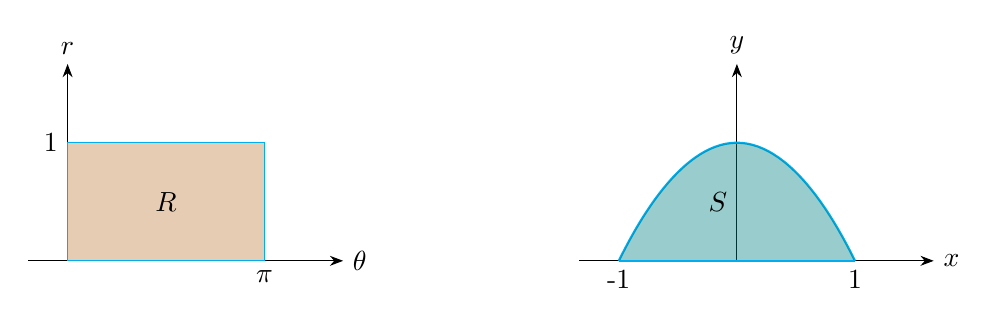
\begin{tikzpicture}[=>stealth]
\draw[-Stealth](-0.5,0)--(3.5,0)node[right]{$\theta$};
\draw[-Stealth](0,0)--(0,2.5)node[above]{$r$};
\path[fill=brown,opacity=0.4](0,0)--(2.5,0)--(2.5,1.5)--(0,1.5)--cycle;
\draw[cyan](0,0)rectangle(2.5,1.5);
\draw(2.5,0)node[below]{$\pi$}
(0,1.5)node[left]{$1$}
(1.25,0.75)node[]{$R$};
\draw[-Stealth](6.5,0)--(11,0)node[right]{$x$};
\draw[-Stealth](8.5,0)--(8.5,2.5)node[above]{$y$};
\draw[thick,cyan](8.5,1.5)parabola(10,0);
\draw[thick,cyan](8.5,1.5)parabola(7,0);
\path[fill=teal,opacity=0.4](8.5,1.5)parabola(10,0)--(8.5,0)--(8.5,1.5)parabola(7,0)--(8.5,0);
\draw[thick,cyan](7,0)--(10,0);
\draw(7,0)node[below]{-1}
(10,0)node[below]{1}
(8.5,0.75)node[left]{$S$};
\end{tikzpicture}
\end{figure}

$$S = \big\{(x,y)\hspace{0.1cm}: \hspace{0.1cm} x = r\cos \theta \hspace{0.1cm} , \hspace{0.1cm} y = r\sin \theta.\hspace{0.2cm} 0 \leq r\leq 1 \hspace{0.1cm} , 0\leq \theta \leq \pi \big\}$$


Recall: A mapping $f: \mathbb{R}^n \longrightarrow \mathbb{R}^m$ is called a linear transformation if
\begin{enumerate}
\item $f(x+y) = f(x) + f(y)\hspace{1cm} x,y, \in \mathbb{R}^n$

\item $f(\alpha x) = \alpha f(x)$, $\hspace{0.2cm} \alpha$ a scalar $x \in \mathbb{R}^n$
\end{enumerate}

If $f$ is a linear transformation from $\mathbb{R}^n$ to $\mathbb{R}^m$ , then there exists an $m\times n$ matrix $A$ such that $$f(x) = Ax$$
\end{exa}


\begin{exa}


Given $f$ and $g$
$$f(x,y,z) =\begin{pmatrix}
\sqrt{1 - x^2 - y^2 -z^2} & , & xy^2z^3\\
\end{pmatrix}
$$

$$g(x,y,z) = \begin{pmatrix}
\dfrac{1}{x + y + z} & , & \sqrt{x}\\
\end{pmatrix}
$$

$$f: \mathbb{R}^3 \longrightarrow \mathbb{R}^2\hspace{0.5cm}, \hspace{0.5cm} g: \mathbb{R}^3 \longrightarrow \mathbb{R}^2$$

Compute $-4f$ and $f+g$ and determine their domains.


$$\text{Domain of }\hspace{0.2cm} f = \big\{(x,y,z)\hspace{0.1cm}:\hspace{0.1cm} x^2 + y^2 + z^2 \leq 1\big\}$$

$$-4f =\begin{pmatrix}
-4\sqrt{1 - x^2 - y^2 -z^2} & , & -4 xy^2z^3\\
\end{pmatrix}
$$

$$\implies \hspace{0.5cm} \text{Domain of }\hspace{0.3cm} -4f = \hspace{0.3cm} \text{Domain of }\hspace{0.4cm} f.$$


$$f +g =\begin{pmatrix}
\sqrt{1 - x^2 - y^2 -z^2} + \dfrac{1}{x + y + z} & , & xy^2z^3 + \sqrt{x}\\
\end{pmatrix}
$$

$$\text{Domain of } \hspace{0.3cm} f+ g = \big\{ (x,y,z)\hspace{0.1cm} : \hspace{0.1cm} x^2 + y^2 + z^2 \leq 1 \hspace{0.1cm}, \hspace{0.1cm} x+y+z\neq 0\hspace{0.1cm},\hspace{0.1cm} x\geq 0\big\}$$
\end{exa}


\begin{defn}


Let $f: \mathbb{R}^n \longrightarrow \mathbb{R}^m$ be differentiable at a point $\underline{X}$ in $\mathbb{R}^n$.
Then the Jacobian of the mapping is the determinant of the Jacobian matrix.
\end{defn}


\begin{defn}


Let $f: \mathbb{R}^n \longrightarrow \mathbb{R}^n$ be in $C^1\big(\Omega\big)$ for some open set $\Omega$ in $\mathbb{R}^n$.\\ Then $f$ is said to be locally $C^1$ invertible on $\Omega$ if there exists a function $g: \mathbb{R}^n \longrightarrow \mathbb{R}^n$ which is in $C^1\big(f(\Omega)\big)$ such that $\big(gof\big) (x) = x$ for every $x\in \Omega$.


$\big(fog\big)(y) = y$ for every $y \in f\big(\Omega\big)$ i.e $g = f^{-1}$.


Invertibility of a linear transformation $f^{-1}(x) = A^{-1}(x)$ since $f(x) = A x$.
\end{defn}


{\color[wave]{485}\subsection{Inverse Function Theorem}}
Let $f: \mathbb{R}^n \longrightarrow \mathbb{R}^n$ be in $C^1\big(\Omega\big)$ on an open set $\Omega$ and let $x_0$ be in $\Omega$ if the Jacobian determinant $\big(\det J_{f(x_0)} \neq 0 \big)$ is not zero, then there is an open set $\Omega_1 \subseteq \Omega$ such that $x_0 \in \Omega_1$ and $f$ is locally $C^1-$ invertible on $\Omega_1$ moreover if $g = f^{-1}$ on $f\big(\Omega\big)$ then $$J_{f^{-1}(x_0)} = J_{g(x_0)} = \Big(J_{f(x_0)}\Big)^{-1}$$


\begin{exa}


Let $f: \mathbb{R}^n$ to $\mathbb{R}^n$ be the polar transformation $\hspace{0.3cm} x = r\cos \theta\hspace{0.2cm},\hspace{0.2cm} y = r\sin \theta$
\end{exa}


\begin{solution}
$$f_1 (r,\theta) = r \cos \theta \hspace{1cm} f_2(r,\theta) = r \sin \theta$$

\begin{align*}
\frac{\partial (f_1,f_2)}{\partial(r,\theta)} & = \begin{vmatrix}
\dfrac{\partial f_1}{\partial r} & \dfrac{\partial f_1}{\partial \theta}\\\\
\dfrac{\partial f_2}{\partial r} & \dfrac{\partial f_2}{\partial \theta}\\
\end{vmatrix}\\\\
& = \begin{vmatrix}
\cos \theta & - r\sin \theta\\
\sin \theta & r\cos \theta \\
\end{vmatrix}\\
& = r\\
\end{align*}

$$ J_{f(r,\theta)} =  \begin{pmatrix}
\cos \theta & - r\sin \theta\\
\sin \theta & r\cos \theta \\
\end{pmatrix}$$\\

\begin{align*}
\big[J_{f(r,\theta)}\big]^{-1} & = \frac{1}{r}\begin{pmatrix}
r\cos \theta & r \sin \theta \\
-\sin \theta & \cos \theta\\
\end{pmatrix}\\\\
& = 
\begin{pmatrix}
\cos \theta & \sin \theta\\
\dfrac{-\sin \theta}{r} & \dfrac{\cos \theta}{r}\\
\end{pmatrix}\\\\
\end{align*}
\end{solution}

{\color[wave]{485}\subsection{Functional Dependence}}
Let $u(x,y)$ and $v(x,y)$. If $u = g(v)$ or $v = h(u)$, then $u$ and $v$ are functionally dependent. If functional dependence between $u$ and $v$ exists, then we can consider $f(u,v) = 0$.

\begin{align*}
\text{So}\hspace{1cm} \frac{\partial f}{\partial u}\cdot \frac{\partial u}{\partial x} + \frac{\partial f}{\partial v}\cdot \frac{\partial v}{\partial x} & = 0\\\\
\frac{\partial f}{\partial u}\cdot \frac{\partial u}{\partial y} +  \frac{\partial f}{\partial v}\cdot \frac{\partial v}{\partial y} & = 0\\
\end{align*}

$$\begin{pmatrix}
\dfrac{\partial u}{\partial x} & \dfrac{\partial v}{\partial x}\\\\
\dfrac{\partial u}{\partial y} & \dfrac{\partial v}{\partial y}\\
\end{pmatrix}
\begin{pmatrix}
\dfrac{\partial f}{\partial u}\\\\
\dfrac{\partial f}{\partial v}\\
\end{pmatrix}
 = 0
$$

Since we desire a non-trivial solution, the determinant of the coefficient matrix must be zero for functional dependency.
$$\text{i.e}\hspace{1cm}
\begin{vmatrix}
\dfrac{\partial u}{\partial x} & \dfrac{\partial v}{\partial x}\\\\
\dfrac{\partial u}{\partial y} & \dfrac{\partial v}{\partial y}\\
\end{vmatrix} = 0$$

but $\det A = \det A^T$


$\therefore\hspace{0.4cm}$ the equation is equivalent 
$$
\begin{vmatrix}
\dfrac{\partial u}{\partial x} & \dfrac{\partial v}{\partial x}\\\\
\dfrac{\partial u}{\partial y} & \dfrac{\partial v}{\partial y}\\
\end{vmatrix} = 0 \iff J = \frac{\partial (u,v)}{\partial (x,y)} = 0
$$


\begin{exa}


Determine if the following  are functionally dependent.
\begin{align*}
u & =  x  +  z\\
v & =  x  +  2z^2\\
w & =  x  -  4yz - 2y^2\\
\end{align*}
\end{exa}

\begin{solution}
\begin{align*}
\frac{\partial (u,v,w)}{\partial (x,y,z)} & = \begin{vmatrix}
\dfrac{\partial u}{\partial x} & \dfrac{\partial u}{\partial y} & \dfrac{\partial u}{\partial z}\\\\
\dfrac{\partial v}{\partial x} & \dfrac{\partial v}{\partial y} & \dfrac{\partial v}{\partial z}\\\\
\dfrac{\partial w}{\partial x} & \dfrac{\partial w}{\partial y} & \dfrac{\partial w}{\partial z}\\
\end{vmatrix}
= \begin{vmatrix}
0 & 1 & 1\\
1 & 0 & 4z\\
1 & -4z - 4y & -4y\\
\end{vmatrix}\\\\
& = 0
\end{align*}

$\therefore\hspace{0.4cm} u,v,w$ are functionally dependent, in fact $w = v - 2u^2$ (check).
\end{solution}


\begin{exa}


Determine if the following are functionally dependent.
\begin{align*}
f(x,y) & = e^x \sin y\\
g(x,y) & = x + \log \sin y\\
\end{align*}
\end{exa}

\begin{solution}
\begin{align*}
\text{So}\hspace{1cm} \frac{\partial (f,g)}{\partial (x,y)} & = \begin{vmatrix}
\dfrac{\partial f}{\partial x} & \dfrac{\partial f}{\partial y}\\\\
\dfrac{\partial g}{\partial x} & \dfrac{\partial g}{\partial y}\\ 
\end{vmatrix} = \begin{vmatrix}
e^x\sin y & e^x\cos y\\
1 & \cot y\\
\end{vmatrix}\\\\
& = e^x\cos y - e^x\cos y\\
& = 0
\end{align*}
$f$ and $g$ are functionally dependent, in fact $(\log f - g = 0)$.


\pagebreak
\end{solution}
{\color[wave]{485}\section{Surfaces}}

Recall $$Ax^2 + Bxy + Cy^2 + Dx + Ey + F = 0$$
In three dimensions, the graph of a second degree equation in $x,y,z$

$$Ax^2 + By^2 + Cz^2 + Exy + Fyz + Gxz + Hx + Iy + Jz + K =0$$ is a quadric (or quadratic) surface (expect for degenerate cases).


 We will consider the case where $E = G = F =0$.


 The trace of a surface is the intersection of that surface with the plane.


\begin{exa}


Use traces to sketch the graph of the function $z = f(x,y) = 4x^2 + y^2$.

$$x = 0\hspace{0.5cm} z = y^2$$

$$ x = k\hspace{0.5cm} z = 4K^2 + y^2$$

% DIAGRAM 16

\begin{figure}[H]
\centering
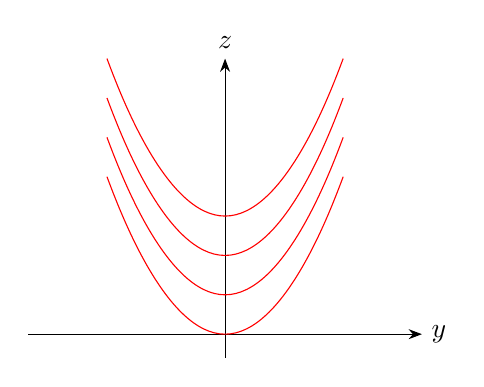
\begin{tikzpicture}[=>stealth]
\draw[-Stealth](-2.5,0)--(2.5,0)node[right]{$y$};
\draw[-Stealth](0,-0.3)--(0,3.5)node[above]{$z$};
\draw[red](0,0)parabola(1.5,2)
(0,0)parabola(-1.5,2)
(0,0.5)parabola(1.5,2.5)
(0,0.5)parabola(-1.5,2.5)
(0,1)parabola(1.5,3)
(0,1)parabola(-1.5,3)
(0,1.5)parabola(1.5,3.5)
(0,1.5)parabola(-1.5,3.5);
\end{tikzpicture}
\end{figure}

any plane parallel $yz$ intersects the surface is parabola.

$$y = 0 \hspace{0.5cm} z = 4x^2$$
$$y=k \hspace{0.5cm} z = 4x^2 + K^2$$

% DIAGRAM 18

\begin{figure}[H]
\centering
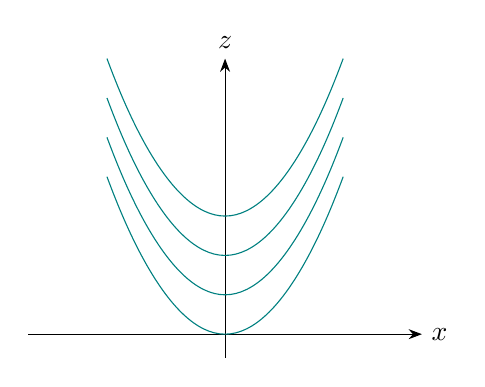
\begin{tikzpicture}[=>stealth]
\draw[-Stealth](-2.5,0)--(2.5,0)node[right]{$x$};
\draw[-Stealth](0,-0.3)--(0,3.5)node[above]{$z$};
\draw[teal](0,0)parabola(1.5,2)
(0,0)parabola(-1.5,2)
(0,0.5)parabola(1.5,2.5)
(0,0.5)parabola(-1.5,2.5)
(0,1)parabola(1.5,3)
(0,1)parabola(-1.5,3)
(0,1.5)parabola(1.5,3.5)
(0,1.5)parabola(-1.5,3.5);
\end{tikzpicture}
\end{figure}

\vspace{3cm}

$$z =0 \hspace{0.5cm} 0 = 4x^2 + y^2$$
$$z =K \hspace{0.5cm} K = 4x^2 + y^2$$

% DIAGRAM 17

\begin{figure}[H]
\centering
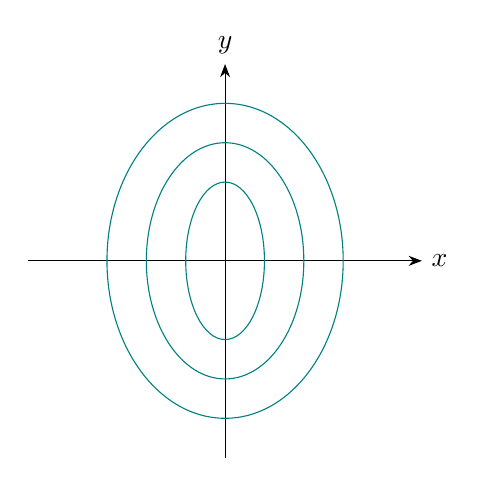
\begin{tikzpicture}[=>stealth]
\draw[-Stealth](-2.5,0)--(2.5,0)node[right]{$x$};
\draw[-Stealth](0,-2.5)--(0,2.5)node[above]{$y$};
\draw[teal](0,0)ellipse[x radius = 0.5cm, y radius=1cm]
(0,0)ellipse [x radius = 1cm, y radius = 1.5cm]
(0,0) ellipse [ x radius = 1.5cm , y radius = 2cm];
\end{tikzpicture}
\end{figure}

% DIAGRAM 19

\begin{figure}[H]
\centering
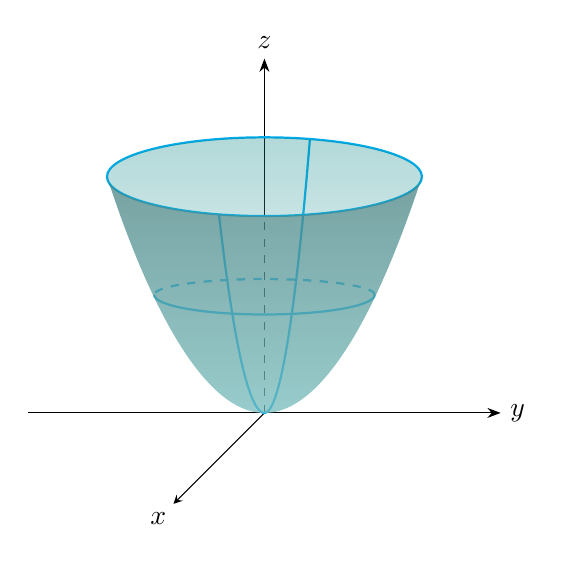
\begin{tikzpicture}[=>stealth]
\draw[-Stealth](-3,0,0)--(3,0,0)node[right]{$y$};
\draw[-Stealth](0,2.5,0)--(0,4.5,0)node[above]{$z$};
\draw[-stealth](0,0,0)--(0,0,3);
\draw(0,0,3.5)node[]{$x$};
\draw[dashed](0,0,0)--(0,2.5,0);
%\draw(0,0)parabola(2,3)
%(0,0)parabola(-2,3);
\draw[cyan,thick](2,3)arc(0:360:2cm and 0.5cm)
(0,0,0)parabola(0,3.1,1.5)
(0,0,0)parabola(0,2.9,-1.5)
(-1.4,1.5)arc(180:360:1.4cm and 0.25cm);
\draw[dashed,thick,cyan](1.4,1.5)arc(0:180:1.4cm and 0.2cm);
\shade[top color=teal,opacity=0.3](2,3)arc(0:180:2cm and 0.5cm)--(-2,3)parabola[bend at end](0,0)--(0,0)parabola(2,3)--cycle;
\shade[top color=teal,opacity=0.4](-2,3)arc(180:360:2cm and 0.5cm)--(2,3)parabola[bend at end](0,0)--(0,0)parabola(-2,3)--cycle;
\shade[bottom color=teal,opacity=0.4](-2,3)arc(180:360:2cm and 0.5cm)--(2,3)parabola[bend at end](0,0)--(0,0)parabola(-2,3)--cycle;
\end{tikzpicture}
\end{figure}
\end{exa}

\begin{exa}


Sketch the quadric surface
$$ x^2 + \frac{y^2}{9} + \frac{z^2}{4} =1$$
\end{exa}


\begin{solution}


The traces in the $yz$ plane

$$x =0 \hspace{1cm} \frac{y^2}{9} + \frac{z^2}{4} = 1$$
% DIAGRAM

$$x =K\hspace{1cm} \frac{y^2}{9}+ \frac{z^2}{4} = 1 -K^2$$
this is an ellipse $K^2\leq 1$


% DIAGRAM 

$$ y = 0\hspace{1cm} x^2 + \frac{z^2}{4} =1$$
% DIAGRAM
$$y = K\hspace{1cm} x^2 + \frac{z^2}{4} = 1-\frac{K^2}{9}\hspace{0.5cm} K^2\leq 9$$

$$z = 0\hspace{1cm} x^2 + \frac{y^2}{9} =1$$
$$ z =k\hspace{1cm} x^2 + \frac{y^2}{9} = 1- \frac{K^2}{4}\hspace{0.5cm} K^2 \leq 4$$

% DIAGRAM 20

\begin{figure}[H]
\centering
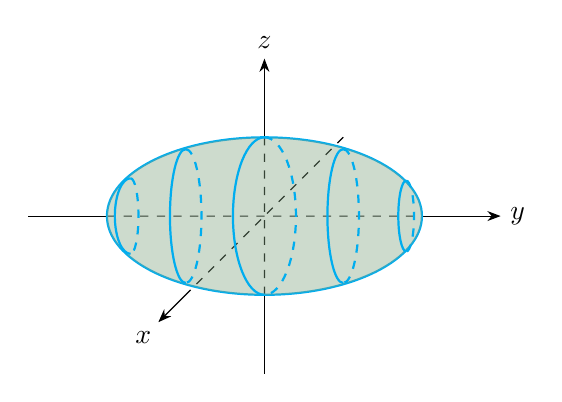
\begin{tikzpicture}[=>stealth]
\draw[-Stealth](2,0,0)--(3,0,0)node[right]{$y$};
\draw[-Stealth](0,1,0)--(0,2,0)node[above]{$z$};
\draw[-Stealth](0,0,2.6)--(0,0,3.5);
\draw[dashed](-2,0,0)--(2,0,0)
(0,-1,0)--(0,1,0)
(0,0,-2.6)--(0,0,2.6);
\draw(0,0,4)node[]{$x$}
(-3,0,0)--(-2,0,0)
(0,-2,0)--(0,-1,0);
\draw[thick,cyan](2,0)arc(0:360:2cm and 1cm);
\path[fill=cyan!50!orange,opacity=0.4](2,0)arc(0:360:2cm and 1cm);
\draw[dashed,thick,cyan](0,1)arc(90:-90:0.4cm and 1cm)
(1,0.85)arc(90:-90:0.2cm and 0.85cm)
(-1,0.85)arc(90:-90:0.2cm and 0.85cm)
(1.8,0.45)arc(90:-90:0.1cm and 0.45cm)
(-1.7,0.48)arc(90:-90:0.1cm and 0.48cm);
\draw[thick,cyan](0,1)arc(90:270:0.4cm and 1cm)
(1,0.85)arc(90:270:0.2cm and 0.85cm)
(-1,0.85)arc(90:270:0.2cm and 0.85cm)
(1.8,0.45)arc(90:270:0.1cm and 0.45cm)
(-1.7,0.48)arc(90:270:0.2cm and 0.48cm);
\end{tikzpicture}
\end{figure}
\end{solution}

\begin{exa}


Classify the quadratic equation 
$$x^2 + 2z^2 - 6x -y + 10 =0$$

$$ x^2 -6x + 9 + 2z^2 -y + 10 -9 =0$$

$$(x-3)^2 + 2z^2 -y + 1 =0$$

$$y-1 = (x-3)^2 + 2z^2$$

$$Y = X^2 + 2Z^2$$

% DIAGRAM 21

\begin{figure}[H]
\centering
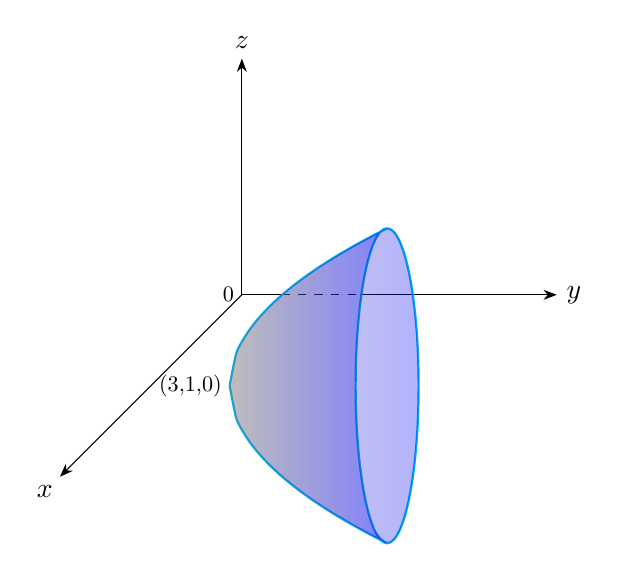
\begin{tikzpicture}[=>stealth]
\draw[-Stealth](0.5,0,-3)--(3,0,-3)node[right]{$y$};
\draw[-Stealth](-1,0,-3)--(-1,3,-3)node[above]{$z$};
\draw[-Stealth](-1,0,-3)--(-1,0,3);
\draw(-1,0,3.5)node[]{$x$}
(-1,0,-3)--(-0.5,0,-3)
(-1,0,-3)node[left,scale=0.8]{0}
(0,0,0)node[left,scale=0.8]{(3,1,0)};
\draw[dashed](-0.5,0,-3)--(0.5,0,-3);
\draw[smooth,domain=0:2,variable=\x,thick,cyan]plot(\x,{sqrt(2*\x)});
\draw[smooth,domain=0:2,variable=\x,thick,cyan]plot(\x,{-sqrt(2*\x)});
\draw[cyan,thick](2,2)arc(90:450:0.4cm and 2cm);
\shade[right color=blue,opacity=0.3,smooth,domain=0:2,variable=\x]plot(\x,{sqrt(2*\x)})--(2,2)arc(90:-90:0.4cm and 2cm)--plot(\x,{-sqrt(2*\x)})--cycle;
\shade[right color=blue,opacity=0.3,smooth,domain=0:2,variable=\x]plot(\x,{sqrt(2*\x)})--(2,2)arc(90:270:0.4cm and 2cm)--plot(\x,{-sqrt(2*\x)})--cycle;
\end{tikzpicture}
\end{figure}

Cone: $\displaystyle{\frac{z^2}{c^2}=\frac{y^2}{a^2} + \frac{y^2}{b^2}}$
\end{exa}


\begin{exe}


\hspace{0.3cm} Sketch the graph of
\begin{enumerate}
\item $16x^2 - 9y^2 + 36z^2 = 144$

\item $y^2 + 4z^2 =x$
\end{enumerate} 
Use traces of the functions and sketch the graphs.
\end{exe}


{\color[wave]{485}\subsection{Surface of Revolution}}
A surface of revolution is obtained by revolving a plane $C$ about a line (axis of revolution) in the plane.\\ The graph of $f(x,y)=0$ in the $xy$ plane is a curve $C$.

% DIAGRAM 22

\begin{figure}[H]
\centering
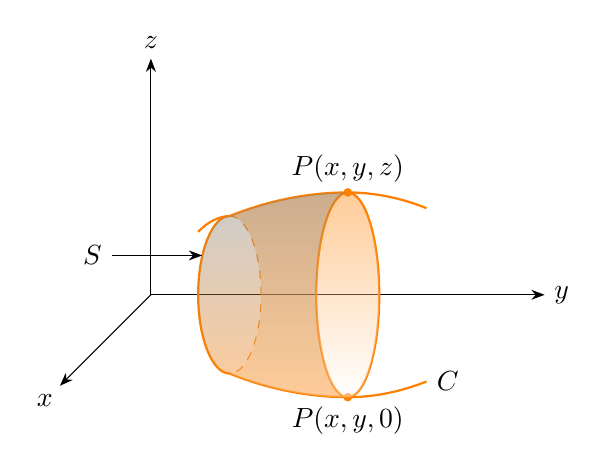
\begin{tikzpicture}[=>stealth]
\draw[-Stealth](0,0,0)--(5,0,0)node[right]{$y$};
\draw[-Stealth](0,0,0)--(0,3,0)node[above]{$z$};
\draw[-Stealth](0,0,0)--(0,0,3);
\draw(0,0,3.5)node[]{$x$};
\draw[orange,thick](2.5,1.3)arc(90:450:0.4cm and 1.3cm)
(1,1)arc(90:270:0.4cm and 1cm)
(1,1)parabola[bend at end](2.5,1.3)
(2.5,1.3)parabola(3.5,1.1)
(1,1)parabola(0.6,0.8)
(1,-1)parabola[bend at end](2.5,-1.3)
(2.5,-1.3)parabola(3.5,-1.1)node[right,black]{$C$};
\draw[-Stealth](-0.5,0.5)--(0.65,0.5);
\draw[dashed,orange](1,1)arc(90:-90:0.4cm and 1cm);
\draw(2.5,1.3)node[shape=circle,fill=orange,draw=orange,scale=0.01cm]{}
(2.5,-1.3)node[shape=circle,fill=orange,draw=orange,scale=0.01cm]{}
(2.5,1.3)node[above]{$P(x,y,z)$}
(2.5,-1.3)node[below]{$P(x,y,0)$}
(-0.5,0.5)node[left]{$S$};
\shade[top color=orange,opacity=0.4](2.5,1.3)arc(90:-90:0.4cm and 1.3cm)--(2.5,-1.3)--(2.5,-1.3)parabola(1,-1)--(1,-1)arc(270:450:0.4cm and 1cm)--(1,1)--(1,1)parabola[bend at end](2.5,1.3)--cycle;
\shade[bottom color=orange, opacity=0.4](2.5,1.3)arc(90:270:0.4cm and 1.3cm)--(2.5,-1.3)--(2.5,-1.3)parabola(1,-1)--(1,-1)arc(-90:-270:0.4cm and 1cm)--(1,1)--(1,1)parabola[bend at end](2.5,1.3)--cycle;
\end{tikzpicture}
\end{figure}

A point $P(x,y,z)$ is on $S$ if and only if $Q(x,y,0)$ is on $C$, and $x_1 = \sqrt{x^2 + y^2}$. Consequently, $P(x,y,z)$ is  on $S$ if and only if $f\big(\sqrt{x^2 + y^2}, y\big) = 0$.


Thus to find an equation for $S$, we replace the variable $x$ by $\sqrt{x^2 + y^2}$.


Similarly, if the graph of $f(x,y) =0$ is revolved about the $x-$ axis then for the resulting surface may be found by replacing $y$ by $\sqrt{y^2 + z^2}$


For curves that contain points $(x,y)$ with $x$ or $y$ negative can be extended by substituting $\pm \sqrt{x^2 + y^2}$ for $x$ or $\pm \sqrt{y^2 + z^2}$ for $y$.


\begin{exa}


The graph of $9x^2 + 4y^2 = 36$ is revolved about the $y-$ axis . Find an equation for the resulting surface.

% DIAGRAM 23

\begin{figure}[H]
\centering
\begin{tikzpicture}[=>stealth]
\draw[-Stealth](-2,0)--(2,0)node[right]{$x$};
\draw[-Stealth](0,-2)--(0,2)node[above]{$y$};
\draw[thick,cyan](0,0)ellipse[x radius = 0.8cm, y radius = 1.6cm];
\end{tikzpicture}
\end{figure}

$$9x^2 + 4y^2 = 36$$

$$9\big(\sqrt{x^2 + y^2}\big)^2 + 4y^2 = 36$$

$$ 9x^2 + 9z^2 + 4y^2 = 36$$
\end{exa}


\begin{exa}


Find a generating curve and the axis of revolution for the surface given by $x^2 + 3y^2 + z^2 = 9$
\end{exa}


\begin{solution}


Because the coefficients of $x^2$ and $z^2$ are equal we choose the form $$x^2 + z^2 = 9 - 3y^2$$
The $y-$ axis is the axis of revolution you can choose a generating curve from either of the following traces

$$x^2 = 9 -3y^2$$

$$z^2 = 9 - 3y^2$$

\begin{align*}
f(x,y) = 0 \hspace{1cm} & x \hspace{0.5cm} \text{replace}\hspace{0.5cm} y \hspace{0.5cm} \text{by}\hspace{0.5cm} \sqrt{y^2 + z^2}\\
& y \hspace{0.5cm} \text{replace}\hspace{0.5cm} x \hspace{0.5cm} \text{by}\hspace{0.5cm} \sqrt{x^2 + z^2}\\
\end{align*}

\begin{align*}
g(y,z) =0\hspace{1cm} & y \hspace{0.5cm} \text{replace}\hspace{0.5cm} z \hspace{0.5cm} \text{by}\hspace{0.5cm} \sqrt{y^2 + z^2}\\
& z \hspace{0.5cm} \text{replace}\hspace{0.5cm} y \hspace{0.5cm} \text{by}\hspace{0.5cm} \sqrt{y^2 + x^2}\\
\end{align*}

\begin{align*}
h(x,z) = 0 \hspace{1cm} & x \hspace{0.5cm} \text{replace}\hspace{0.5cm} z \hspace{0.5cm} \text{by}\hspace{0.5cm} \sqrt{y^2 + z^2}\\
& z \hspace{0.5cm} \text{replace}\hspace{0.5cm} x \hspace{0.5cm} \text{by}\hspace{0.5cm} \sqrt{x^2 + y^2}\\\\
\end{align*}

\pagebreak
\end{solution}

{\color[wave]{485}\subsection{Cylindrical and Spherical Coordinates}}
In three dimensions, there are two coordinates systems that give convenient descriptions of some common occurring surfaces and solids.


\subhead{Cylindrical Coordinates}

% DIAGRAM 27

\begin{figure}[H]
\centering
\begin{tikzpicture}[=>stealth]
\draw[-Stealth](-0.5,0,0)--(4,0,0)node[right]{$y$};
\draw[-Stealth](0,-0.5,0)--(0,3,0)node[above]{$z$};
\draw[-Stealth](0,0,-0.5)--(0,0,4);
\draw(0,0,4.5)node[]{$x$}
(-0.3,0,0)node[above]{0}
(3,0,3)node[shape=circle,fill=red,scale=0.01cm]{}
(3,3,3)node[shape=circle,fill=red,scale=0.01cm]{}
(3,3,3)node[above,scale=0.9]{$P(r,\theta, z)$}
(3,0,3)node[right,scale=0.9]{$(r,\theta,0)$}
(3,1.5,3)node[right]{$z$}
(1.5,0,1.5)node[above]{$r$};
\draw[red](0,0,0)--(3,0,3);
\draw[red](3,0,3)--(3,3,3);
\coordinate (a) at (0,0,0.5);
\coordinate (b) at (0,0,0);
\coordinate (c) at (0.5,0,0.5);
\draw
pic[draw = red, angle radius = 0.5cm, ->, "$\theta$", angle eccentricity=1.4]{angle = a--b--c};
\draw(2.8,0,2.8)--(2.8,0.2,2.8)--(3,0.2,3)
(0,0,2.7)--(0.3,0,2.7)--(0.3,0,3)
(2.7,0,0)--(2.7,0,0.3)--(3,0,0.3);
\draw[dashed,cyan](0,0,3)--(2.97,0,3)
(3,0,2.97)--(3,0,0);
\end{tikzpicture}
\end{figure}

$$x = r\cos \theta\hspace{0.3cm}, \hspace{1cm} y = r\sin \theta \hspace{0.3cm},\hspace{1cm} z =z$$

where as to convert from rectangular to cylindrical coordinates we use $$r^2 = x^2 + y^2\hspace{0.2cm}, \hspace{1cm} \tan \theta = \frac{y}{x}\hspace{0.2cm},\hspace{1cm} z =z$$

Cylindrical coordinates are useful in problems that involve symmetry about some axis and the $z-$axis is chosen to coincide with the axis of symmetry.


\begin{exa}


Describe the surface whose equation in cylindrical coordinates is $z = r$.
\end{exa}


\begin{solution}


$z =r$


$z = r^2 = x^2 + y^2$


$z^2 = x^2 + y^2$


Cone, with axis of symmetry $z$ axis.
\end{solution}


\begin{exa}


Find an equation in cylindrical coordinates for the ellipsoid $$4x^2 + 4y^2 + z^2 =1$$
\end{exa}


\begin{solution}


$r^2 = x^2 + y^2$

\begin{align*}
4(x^2 + y^2) + z^2 & =1\\
4r^2 + z^2 & =1\\\\
\therefore\hspace{0.5cm}z^2 & = 1 - 4r^2\\\\
\end{align*}
\end{solution}

\subhead{Spherical Coordinates}


The spherical coordinate $(\rho, \theta, \phi)$ of a point $P$  is space is shown below:-

% DIAGRAM 28

\begin{figure}[H]
\centering
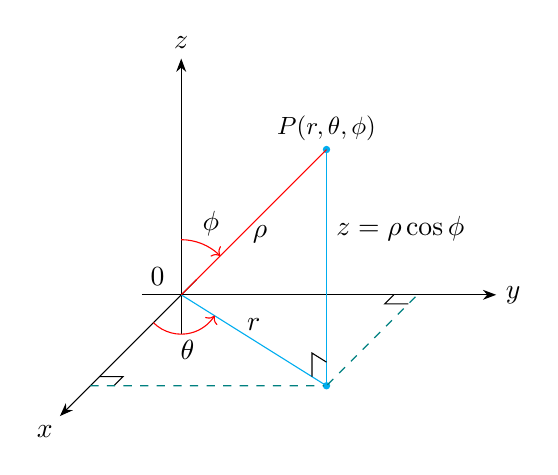
\begin{tikzpicture}[=>stealth]
\draw[-Stealth](-0.5,0,0)--(4,0,0)node[right]{$y$};
\draw[-Stealth](0,-0.5,0)--(0,3,0)node[above]{$z$};
\draw[-Stealth](0,0,-0.5)--(0,0,4);
\draw(0,0,4.5)node[]{$x$}
(-0.3,0,0)node[above]{0}
(3,0,3)node[shape=circle,fill=cyan,scale=0.01cm]{}
(3,3,3)node[shape=circle,fill=cyan,scale=0.01cm]{}
(3,3,3)node[above,scale=0.9]{$P(r,\theta, \phi)$}
(3,2,3)node[right]{$z=\rho \cos \phi$}
(1.5,0,1.5)node[above]{$r$}
(1,1,0)node[below]{$\rho$};
\draw[cyan](0,0,0)--(3,0,3);
\draw[cyan](3,0,3)--(3,3,3);
\coordinate (a) at (0,0,0.5);
\coordinate (b) at (0,0,0);
\coordinate (c) at (0.5,0,0.5);
\draw
pic[draw = red, angle radius = 0.5cm, ->, "$\theta$", angle eccentricity=1.4]{angle = a--b--c};
\draw(2.7,0,2.7)--(2.7,0.3,2.7)--(3,0.3,3)
(0,0,2.7)--(0.3,0,2.7)--(0.3,0,3)
(2.7,0,0)--(2.7,0,0.3)--(3,0,0.3);
\draw[dashed,teal](0,0,3)--(2.97,0,3)
(3,0,2.97)--(3,0,0);
\draw[red](0,0,0)--(3,3,3);
\coordinate (A) at (0.5,0.5,0);
\coordinate (B) at (0,0.5,0);
\draw
pic[draw = red, angle radius = 0.7cm,<-, "$\phi$", angle eccentricity =1.4]{angle=A--b--B};
\end{tikzpicture}
\end{figure}

where $\rho = \big|OP\big|$ is the distance from the origin to $P$, $\theta$ is same angle as in cylindrical coordinates, and $\phi$ is the angle between the positive $Z-$ axis and the line segment $OP$
$$\rho\geq 0\hspace{0.3cm}, \hspace{0.5cm} 0\leq \theta \leq 2\pi\hspace{0.3cm} , \hspace{0.5cm} 0 \leq \phi \leq \pi$$

To convert from spherical to rectangular coordinates, we use $$x = \rho \sin \phi \cos \theta\hspace{0.4cm} , \hspace{0.4cm} y =\rho \sin \phi \sin \theta\hspace{0.4cm} , \hspace{0.4cm} z = \rho \cos \phi\hspace{0.4cm} \text{and}\hspace{0.4cm} \rho^2 = x^2 + y^2 + z^2$$

$*$ Confirm that $z = \rho \cos \phi$ from $r=\rho \sin \phi$ sketch.


\begin{exa}


Find an equation in spherical coordinates for $x^2 -y^2 -z^2 = 1$.
\end{exa}


\begin{solution}


$x^2 -y^2 -z^2 = 1$

$$\rho^2\sin^2\phi \cos^ \theta - \rho^2 \sin^2\phi \sin^2\theta - \rho^2\cos\phi = 1$$

$$\rho^2\sin^2\phi \big(\cos^2\theta - \sin^2 \theta\big) -\rho^2\cos\phi = 1$$

$$\rho^2\sin^\phi \cos2\theta - \rho^2\cos^\phi =1$$
\end{solution}


\begin{exa}


Find a rectangular equation for the surface whose spherical equation is $\rho = \sin \phi \sin \theta$.
\end{exa}


\begin{solution}
\begin{align*}
x^2 + y^2 + z^2 & = \rho^2\\
x^2 + y^2 +z^2  &  = \rho \sin \phi \sin \theta\\
x^2 + y^2 + z^2 & = y\\
x^2 + y^2 -y + z^2 & = 0\\
x^2 + (y^2 -1/2)^2 + z^2 & = \frac{1}{4}
\end{align*}
which is the equation of sphere with radius $\dfrac{1}{2}$ , centered at $\big(0, 1/2,0\big)$.
\end{solution}


\begin{exa}


The point $\Big( 2, \dfrac{\pi}{4}, \dfrac{\pi}{3}\Big)$ is given in spherical coordinates. Plot the point and find its rectangular coordinates.
\end{exa}


\begin{solution}


$\Big(2,\dfrac{\pi}{4},\dfrac{\pi}{3}\Big)$

$$ x = \rho \sin \phi \cos \theta = 2 \sin \Big(\dfrac{\pi}{3}\Big)\cos \Big(\dfrac{\pi}{4}\Big) = 2\cdot \dfrac{\sqrt{3}}{2}\cdot \frac{1}{\sqrt{2}}=\sqrt{\dfrac{3}{2}}$$

$$y = \rho \sigma \phi \sigma = 2 \sin \Big(\dfrac{\pi}{3}\Big) \sin \Big(\dfrac{\pi}{4}\Big)=2\cdot \dfrac{\sqrt{3}}{2}\cdot \frac{1}{\sqrt{2}}= \sqrt{\dfrac{3}{2}}$$

$$z = \rho \cos \phi = 2\cos \Big(\dfrac{\pi}{3}\Big) = 2 \cdot \frac{1}{2} =1$$
\end{solution}


\begin{exe}


Express $(0,2\sqrt{3},-2)$ given in rectangular coordinates, in spherical coordinates.


\pagebreak
\end{exe}
{\color[wave]{485}\subsection{Tangent Planes}}

% DIAGRAM 29

\begin{figure}[H]
\centering
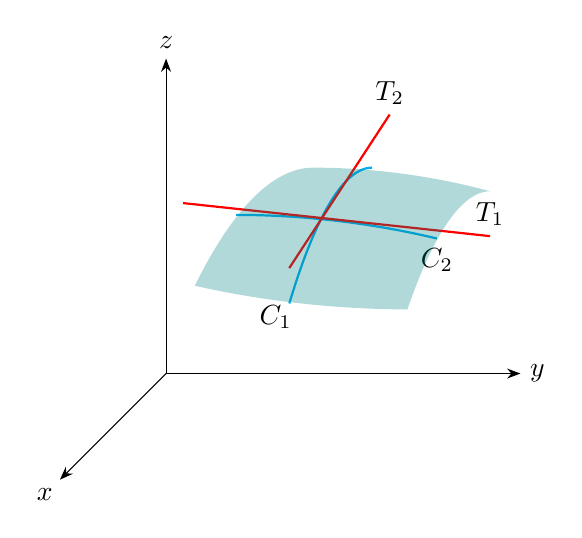
\begin{tikzpicture}[=>stealth]
\draw[-Stealth](0,0,-1)--(4.5,0,-1)node[right]{$y$};
\draw[-Stealth](0,0,-1)--(0,4,-1)node[above]{$z$};
\draw[-Stealth](0,0,-1)--(0,0,2.5);
\draw(0,0,3)node[]{$x$}
%(2.55,1.4)node[right]{$C_2$}
(1.45,1.1)node[right]{$C_1$};
%\draw[scale=1.5,teal](0.5,1)parabola[bend at end](1.5,2)
%(1.5,2)parabola(3,1.8)
%(3,1.8)parabola(2.3,0.8)
%(2.3,0.8)parabola(0.5,1);
\draw[scale=1.5,thick,cyan](1.3,0.85)parabola[bend at end](2,2)
(0.85,1.6)parabola(2.55,1.4)node[black,below]{$C_2$};
\draw[scale=1.5,thick,red](0.4,1.7)--(3,1.42)node[black,above]{$T_1$}
(1.3,1.15)--(2.15,2.45)node[black,above]{$T_2$};
\path[fill=teal,opacity=0.3,scale=1.5](0.5,1)parabola[bend at end](1.5,2)--(1.5,2)parabola(3,1.8)--(3,1.8)parabola(2.3,0.8)--(2.3,0.8)parabola(0.5,1)--cycle;
\end{tikzpicture}
\end{figure}

Let $T_1$ and $T_2$ be tangents to curve $C_1$ and $C_2$. Then the tangent plane to the surface $S$ at the point $P$ is defined to be the plane that contains $T_1$ and $T_2$.


\subhead{Equation of Tangent Plane}


Suppose $f$ has contains first partial derivatives. An equation of the tangent plane to the surface $z = f(x,y)$ at the point $P(x_0, y_0, z_0)$ is $$z -z_0 = f_x(x_0,y_0)(x-x_0) + f_y(x_0,y_0)(y-y_0)$$


\begin{exa}


Find the tangent plane to the elliptic paroboloid $z = 2x^2 + y^2$ at the point $(1,1,3)$.
\end{exa}


\begin{solution}


$z = 2x^2 + y^2 = f(x,y)$


$f_x = 4x\hspace{1cm} f_x(1,1,3) = 4$


$f_y = 2y\hspace{1cm} f_y(1,1,3) = 2$

$$ z -z_0 = f_x(x_0,y_0)(x-x_0) + f_y(x_0,y_0)(y-y_0)$$

$$\implies \hspace{1cm} z - 3 = 4(x-1) + 2(y-1)$$

$$z = 4x + 2y -3$$


\pagebreak
\end{solution}

{\color[wave]{485}\subsection{Parametric Surfaces}}

Suppose that
 $\boxed{\displaystyle{r(u,v) = x(u,v)\,\textbf{i} + y(u,v)\,\textbf{j} + z(u,v)\,\textbf{k}}\hspace{0.3cm}\cdots\cdots\cdots\hspace{0.3cm}(1)}$ is a vector function defined on a region $D$ in the $uv-$ plane.
$x, y, z$ are the component functions of $r$, are functions of $uv$ with domain $D$. The set of points $(x,y,z)$ in $\mathbb{R}^3$ such that
$$x = x(u,v)\hspace{0.4cm},\hspace{0.4cm} y = y(u,v)\hspace{0.4cm}, \hspace{0.4cm} z = z(u,v)\hspace{0.3cm}\cdots\cdots\cdots \hspace{0.3cm}(2)$$ and $(u,v)$ varies throughout $D$ , is called s parametric surface.

% DIAGRAM 30

\begin{table}[H]
\centering
\begin{tabular}{cc}
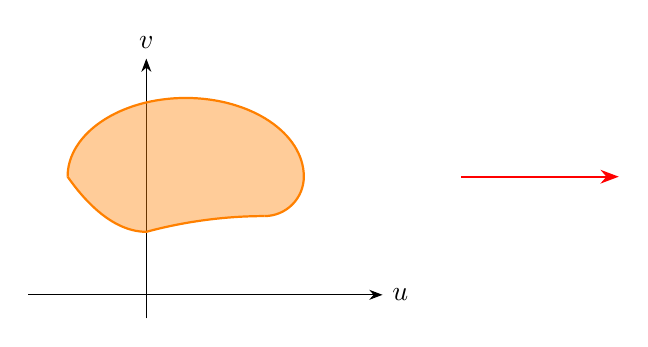
\begin{tikzpicture}[=>stealth]
\draw[-Stealth](-1.5,0)--(3,0)node[right]{$u$};
\draw[-Stealth](0,-0.3)--(0,3)node[above]{$v$};
\draw[thick,orange](2,1.5)arc(0:180:1.5cm and 1cm)
(2,1.5)arc(0:-90:0.5cm and 0.5cm);
%(-1,1.5)parabola[bend at end](0,1)
%(0,1)parabola(1,1.5)
%(1,1.5)parabola(1.5,1);
\draw[thick,orange](0,0.8)parabola[bend at  end](1.5,1)
(-1,1.5)parabola[bend at end](0,0.8);
%\path[fill=orange,opacity=0.4](2,1.5)arc(0:180:1.5cm and 1cm)--(-1,1.5)parabola[bend at end](0,1)--(0,1)parabola(1,1.5)--(1,1.5)parabola(1.5,1)--(1.5,1)arc(270:360:0.5cm and 0.5cm)--cycle;
\path[fill=orange,opacity=0.4](2,1.5)arc(0:180:1.5cm and 1cm)--(-1,1.5)parabola[bend at end](0,0.8)--(0,0.8)parabola[bend at end](1.5,1)--(1.5,1)arc(270:360:0.5cm and 0.5cm)--cycle;
\draw[thick,red,-Stealth](4,1.5)--(6,1.5);
\end{tikzpicture}
&
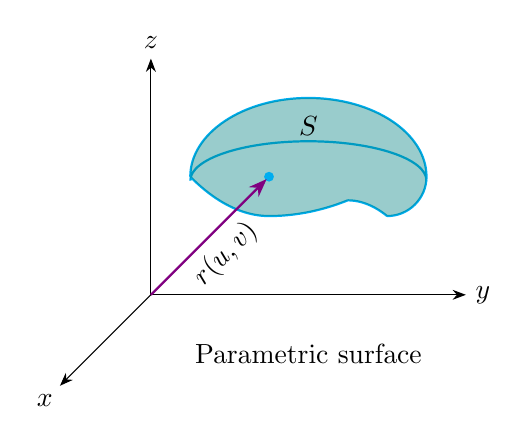
\begin{tikzpicture}[=>stealth]
\draw[-Stealth](0,0,0)--(4,0,0)node[right]{$y$};
\draw[-Stealth](0,0,0)--(0,3,0)node[above]{$z$};
\draw[-Stealth](0,0,0)--(0,0,3);
\draw(0,0,3.5)node[]{$x$};
\draw[thick,cyan](3.5,1.5)arc(0:180:1.5cm and 1cm)
(3.5,1.5)arc(0:-90:0.5cm and 0.5cm)
(0.5,1.5)parabola[bend at end](1.5,1)
(1.5,1)parabola(2.5,1.2)
(2.5,1.2)parabola(3,1)
(0.5,1.45)arc(180:0:1.5cm and 0.5cm);
\path[fill=teal,opacity=0.4](3.5,1.5)arc(0:180:1.5cm and 1cm)--(0.5,1.45)arc(180:0:1.5cm and 0.5cm)--cycle;
\path[fill=teal,opacity=0.4](0.5,1.45)arc(180:0:1.5cm and 0.5cm)--(3.5,1.5)arc(0:-90:0.5cm and 0.5cm)--(3,1)parabola[bend at end](2.5,1.2)--(2.5,1.2)parabola[bend at end](1.5,1)--(1.5,1)parabola(0.5,1.5)--cycle;
\draw(1.5,1.5)node[shape=circle,fill=cyan,scale=0.01cm,draw=cyan,thick]{}
(2,1.9)node[above]{$S$};
\draw[-Stealth,thick,violet](0,0)--node[below,black,sloped]{$r(u,v)$}(1.47,1.47);
\draw(2,-1)node[above]{Parametric surface};
\end{tikzpicture}\\
\end{tabular}
\end{table}

\vspace{1cm}
\begin{exa}


Given $r(u,v) = 2\cos u\, \textbf{i} + v\,\textbf{j} + 2\sin u\, \textbf{k}$. Identify and sketch the surface with the given vector equation.
\end{exa}


\begin{solution}


$x = 2\cos u \hspace{0.4cm}, \hspace{0.4cm} y =v\hspace{0.4cm} , \hspace{0.4cm} z = 2\sin u$

$$x^2 + z^2 = 4\cos^2 u + 4\sin^2 u = 4$$

% DIAGRAM 31

\begin{figure}[H]
\centering
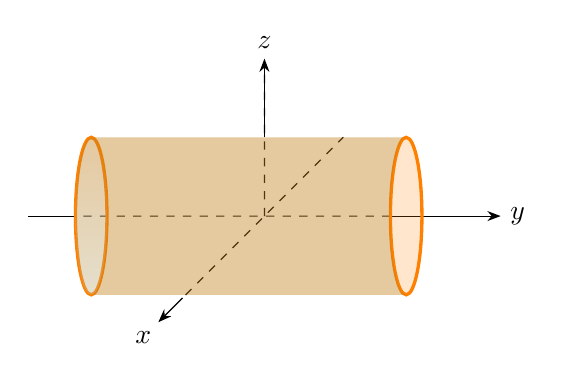
\begin{tikzpicture}[=>stealth]
\draw[-Stealth](1.6,0,0)--(3,0,0)node[right]{$y$};
\draw[-Stealth](0,1,0)--(0,2,0)node[above]{$z$};
\draw[-Stealth](0,0,2.7)--(0,0,3.5);
\draw(0,0,4)node[]{$x$}
(-3,0,0)--(-2.4,0,0);
\draw[dashed]((-2.3,0,0)--(1.6,0,0)
(0,0,0)--(0,1.9,0)
(0,0,2.6)--(0,0,-2.6);
\draw[very thick,orange](2,0,0)arc(0:360:0.2cm and 1cm);
\draw[very thick,orange](-2,0,0)arc(0:360:0.2cm and 1cm);
\path[fill=orange,opacity=0.2](1.8,1,0)arc(90:-90: 0.2cm and 1cm)--(1.8,-1,0)--(-2.2,-1,0)--(-2.2,-1,0)arc(-90:90:0.2cm and 1cm)--(-2.2,1,0)--cycle;
\path[fill=orange,opacity=0.2](-2.2,1,0)arc(90:270: 0.2cm and 1cm)--(-2.2,-1,0)--(1.8,-1,0)--(1.8,-1,0)arc(270:90:0.2cm and 1cm)--(1.8,1,0)--cycle;
\shade[top color=orange,opacity=0.2](-2,0,0)arc(0:360:0.2cm and 1cm);
%%
\path[fill=teal,opacity=0.1](-2.2,1,0)arc(90:270: 0.2cm and 1cm)--(-2.2,-1,0)--(1.8,-1,0)--(1.8,-1,0)arc(270:90:0.2cm and 1cm)--(1.8,1,0)--cycle;
\end{tikzpicture}
\end{figure}

\vspace{1cm}

Suppose that $0\leq u \leq \dfrac{\pi}{2}\hspace{0.4cm}, \hspace{0.4cm} 0 \leq v \leq 3$

$$x\geq 0\hspace{0.5cm} , \hspace{0.5cm} y\leq y \leq 3\hspace{0.5cm} , \hspace{0.5cm} z \geq 0$$

% DIAGRAM 32

\begin{figure}[H]
\centering
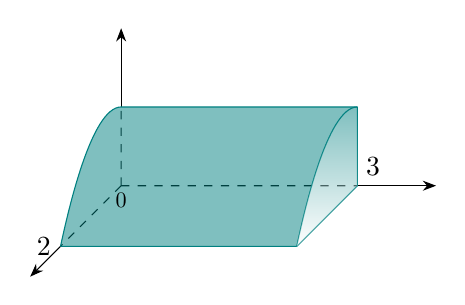
\begin{tikzpicture}[=>stealth]
\draw[-Stealth](3,0,0)--(4,0,0);
\draw[-Stealth](0,1,0)--(0,2,0);
\draw[-Stealth](0,0,2)--(0,0,3);
\draw[dashed](0,0,0)--(3,0,0)
(0,0,0)--(0,1,0)
(0,0,0)--(0,0,2);
\draw[teal](0,1,0)--(3,1,0)
(0,0,2)--(3,0,2)
(3,0,2)--(3,0,0)--(3,1,0);
\draw[teal](0,0,2)parabola[bend at end](0,1,0)
(3,0,2)parabola[bend at end](3,1,0);
\path[fill=teal,opacity=0.5](0,0,2)parabola[bend at end](0,1,0)--(3,1,0)parabola(3,0,2)--(0,0,2)--cycle;
\shade[top color=teal,opacity=0.5](3,1,0)parabola(3,0,2)--(3,0,0)--(3,1,0);
\draw(0,0,0)node[below,scale=0.8]{0}
(0,0,2)node[left]{2}
(3.2,0,0)node[above]{3};
\end{tikzpicture}
\end{figure}
\end{solution}

\begin{exa}


Find a parametric representation of the sphere $x^2 + y^2 + z^2  = 9^2$.
\end{exa}


\begin{solution}


The sphere has a simple representation in spherical coordinates, with $\phi$ and $\theta$ as parameters.


We have that

$$x = a\sin \phi \cos \theta\hspace{0.5cm}, \hspace{0.5cm} y = a\sin \phi\sin \theta\hspace{0.5cm}, \hspace{0.5cm} z = a\cos \phi$$

$$\therefore\hspace{0.4cm} r(\phi, \theta) = a\sin \phi \cos \theta\, \textbf{i} + a \sin \phi \cos \theta\, \textbf{j} + a\cos \phi \,\textbf{k}$$

$$0\leq \phi \leq \pi\hspace{0.5cm}, \hspace{0.5cm} 0\leq \theta \leq 2\pi$$

$$D = [0,\pi]\times [0,2\pi]$$
\end{solution}


{\color[wave]{485}\subsection{Tangent Planes To Parametric Surfaces}}

Given a parametric surface $S$ traced out by a vector equation $$r(u,v) = x(u,v)\, \textbf{i} + y(u,v)\,\textbf{j} + z(u,v)\,\textbf{k}$$ and a point $P$ with position vector $r(u_0,v_0)$. Keeping $u$ constant, $u=u_0$ then $r(u_0,v)$ becomes a vector function of the single parameter $v$, and defines a grid $C_1$ lying on $S$.


Tangent vector to $C_1$ at $P_0$ is $$r_v = \frac{\partial x}{\partial v}(u_0,v_0)\,\textbf{i} + \frac{\partial y}{\partial v}(u_0,v_0)\,\textbf{j} +\frac{\partial z}{\partial v}(u_0,v_0)\,\textbf{k}$$

% DIAGRAM 33

\begin{table}[H]
\centering
\begin{tabular}{cc}
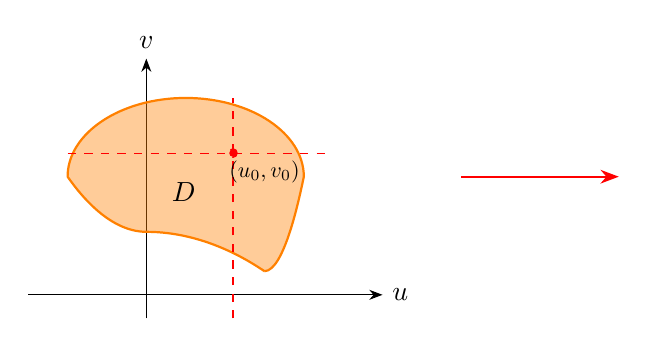
\begin{tikzpicture}[=>stealth]
\draw[-Stealth](-1.5,0)--(3,0)node[right]{$u$};
\draw[-Stealth](0,-0.3)--(0,3)node[above]{$v$};
\draw[thick,orange](2,1.5)arc(0:180:1.5cm and 1cm)
(0,0.8)parabola(1.5,0.3)
(1.5,0.3)parabola(2,1.5)
(-1,1.5)parabola[bend at end](0,0.8);
\path[fill=orange,opacity=0.4](2,1.5)arc(0:180:1.5cm and 1cm)--(-1,1.5)parabola[bend at end](0,0.8)--(0,0.8)parabola(1.5,0.3)--(1.5,0.3)parabola(2,1.5)--cycle;
\draw[thick,red,-Stealth](4,1.5)--(6,1.5);
\draw[dashed,red](1.1,-0.3)--(1.1,2.5)
(-1,1.8)--(2.3,1.8)
(1.1,1.8)node[shape=circle,fill=red,scale=0.01cm,draw=red,thick]{}
(0.2,1.3)node[right,black]{$D$}
(1.5,1.8)node[below,black,scale=0.8]{$(u_0,v_0)$};
\end{tikzpicture}
&
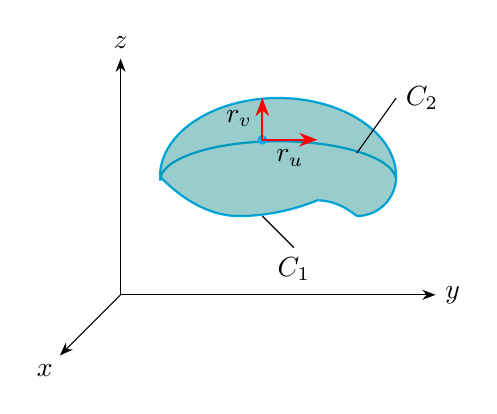
\begin{tikzpicture}[=>stealth]
\draw[-Stealth](0,0,0)--(4,0,0)node[right]{$y$};
\draw[-Stealth](0,0,0)--(0,3,0)node[above]{$z$};
\draw[-Stealth](0,0,0)--(0,0,2);
\draw(0,0,2.5)node[]{$x$};
\draw[thick,cyan](3.5,1.5)arc(0:180:1.5cm and 1cm)
(3.5,1.5)arc(0:-90:0.5cm and 0.5cm)
(0.5,1.5)parabola[bend at end](1.5,1)
(1.5,1)parabola(2.5,1.2)
(2.5,1.2)parabola(3,1)
(0.5,1.45)arc(180:0:1.5cm and 0.5cm);
\path[fill=teal,opacity=0.4](3.5,1.5)arc(0:180:1.5cm and 1cm)--(0.5,1.45)arc(180:0:1.5cm and 0.5cm)--cycle;
\path[fill=teal,opacity=0.4](0.5,1.45)arc(180:0:1.5cm and 0.5cm)--(3.5,1.5)arc(0:-90:0.5cm and 0.5cm)--(3,1)parabola[bend at end](2.5,1.2)--(2.5,1.2)parabola[bend at end](1.5,1)--(1.5,1)parabola(0.5,1.5)--cycle;
\draw(1.8,1.97)node[shape=circle,fill=cyan,scale=0.01cm,draw=cyan,thick]{};
\draw[-Stealth,thick,red](1.8,1.97)--node[below,black,sloped]{$r_u$}(2.5,1.97);
\draw[-Stealth,thick,red](1.8,1.97)--node[left,black,]{$r_v$}(1.8,2.5);
\draw(1.8,1)--(2.2,0.6)node[below]{$C_1$}
(3,1.8)--(3.5,2.5)node[right]{$C_2$};
\end{tikzpicture}\\
\end{tabular}
\end{table}

Similarly  keep $v$ constant, we get a grid $C_2$ given given by $r(u,v_0)$ that lies on $S$ and its tangent is 

$$r_u = \frac{\partial x}{\partial u}(u_0,v_0)\,\textbf{i} + \frac{\partial y}{\partial u}(u_0,v_0)\,\textbf{j} +\frac{\partial z}{\partial u}(u_0,v_0)\,\textbf{k}$$

If $r_u \times r_v$ is not 0, then the surface is smooth. For a smooth surface the tangent plane is the plane that contains the tangent vectors $r_u$, $r_v$ and $r_u \times r_v$ is a normal vector to the tangent place.


\begin{exa}


Find the tangent plane to the surface with parametric equation 
$$x =u^2\hspace{0.4cm},\hspace{0.4cm} y = v^2\hspace{0.4cm} , \hspace{0.4cm} z = u + 2v$$ at the point $(1,1,3)$.
\end{exa}


\begin{solution}


$r(u,v) = u^2 \,\textbf{i} + v^2\,\textbf{j} + (u + 2v)\,\textbf{k}$


$r_u = \dfrac{\partial x}{\partial u}\,\textbf{i} +  \dfrac{\partial y}{\partial u}\,\textbf{j} +  \dfrac{\partial z}{\partial u}\,\textbf{k}$


$r_u = 2u\,\textbf{i} + 0\,\textbf{j} + \textbf{k}$


$\implies\hspace{1cm} r_u = 2u\,\textbf{i} + \textbf{k}$


$$\implies \hspace{1cm} r_v = 2v\,\textbf{j}+ 2\,\textbf{k}$$

Normal vector to the tangent plane is 
\begin{align*}
r_u  \times r_v & = \begin{vmatrix}
\textbf{i} & \textbf{j} & \textbf{k}\\
2u & 0 & 1\\
0 & 2v & 2\\
\end{vmatrix}\\\\
& = -2v\,\textbf{i} -4u\,\textbf{j} + 4uv\,\textbf{k}
\end{align*}
$(1,1,3)$ corresponds to $u=1,\hspace{0.3cm} v =1$


$\therefore$ normal vector is $-2\,\textbf{i} -4\,\textbf{j} + 4\,\textbf{k}.$


$\therefore$ Equation of the tangent plane at $(1,1,3)$ is 
$$-2(x-1) -4(y-1) + 4(z-3) =0$$

$$\implies\hspace{1cm} x+ 2y -2z + 3 = 0$$
\end{solution}


{\color[wave]{485}\subsection{Tangent Planes To Level Curves}}
Suppose $S$ is a surface with equation $F(x,y,z) = K$. Let $C$ to be any curve that lies on $S$ and pass through the point $P$. $C$ is described by a continuous vector function $$r(t) = \langle x(t) \, ,\, y(t)\, , \,z(t)\rangle$$ since $C$ lies on $S$ , any point $(x(t), y(t),z(t))$ must satisfy the equation of $S$ . i.e $$F(x(t)\, ,\, y(t)\, , \,z(t)) = K$$

If $x,y,z$ are differentiable functions at $t$

$$\frac{\partial F}{\partial x}\hspace{0.1cm}\frac{dx}{dt}  +  \frac{\partial F}{\partial y}\hspace{0.1cm}\frac{dy}{dt}    +\frac{\partial F}{\partial z}\hspace{0.1cm}\frac{dz}{dt}  = 0 $$


But since \hspace{0.2cm}$\displaystyle{\nabla f = \langle F_x\, , \,F_y\,  ,\, F_z}\rangle\,$ and $\,\displaystyle{r'(t) = \langle x'(t)\, , \,y'(t)\, , \, z'(t) \rangle}$ $$ \nabla F \cdot r'(t) =0$$

In particular, when $t=t_0$ we have $\displaystyle{r(t_0)  = \langle x_0, y_0, z_0 \rangle}$ $$\nabla F(x_0, y_0,z_0)\cdot r'(t_0) = 0$$ 

% DIAGRAM 34

\begin{figure}[H]
\centering
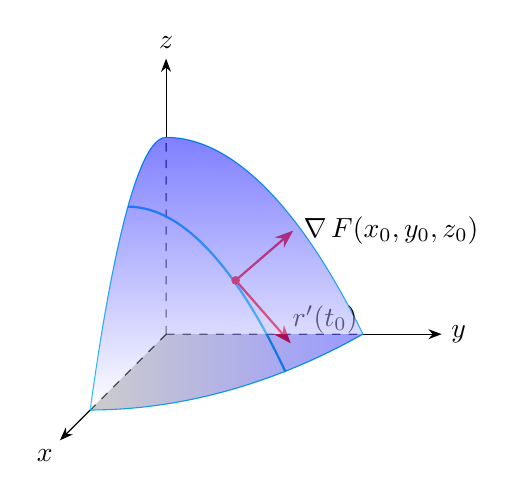
\begin{tikzpicture}[=>stealth]
\draw[-Stealth](2.5,0,0)--(3.5,0,0)node[right]{$y$};
\draw[-Stealth](0,2.5,0)--(0,3.5,0)node[above]{$z$};
\draw[-Stealth](0,0,2.5)--(0,0,3.5);
\draw(0,0,4)node[]{$x$};
\draw[dashed](0,0,0)--(2.5,0,0)
(0,0,0)--(0,2.5,0)
(0,0,0)--(0,0,2.5);
\draw[cyan](2.5,0,0)parabola[bend at end](0,0,2.5)
(0,0,2.5)parabola[bend at  end](0,2.5,0)
(2.5,0,0)parabola[bend at end](0,2.5,0);
\draw[thick,cyan](2,0,1.25)parabola[bend at end](0,2.1,1.25);
\draw(2,1.8,2.9)node[shape=circle,fill=red,draw=red,scale=0.01cm]{};
\draw[-Stealth,thick,red](2,1.8,2.9)--(2,1.7,1)node[right,black]{$\nabla\, F(x_0,y_0,z_0)$};
\draw[-Stealth,thick,red](2,1.8,2.9)--(2.7,1,2.9);
\draw(2.6,1.3,2.9)node[right]{$r'(t_0)$};
\shade[top color=blue,opacity=0.5](0,2.5,0)parabola(2.5,0,0)--(2.5,0,0)--(0,0,0)--(0,2.5,0)--cycle
(0,2.5,0)parabola(0,0,2.5)--(0,0,2.5)--(0,0,0)--(0,2.5,0)--cycle;
\shade[right color=blue,opacity=0.4](2.5,0,0)parabola[bend at end](0,0,2.5)--(0,0,2.5)--(0,0,0)--(2.5,0,0)--cycle;
%\shade[top color=blue,opacity=0.4](0,2.5,0)parabola(2.5,0,0)--(2.5,0,0)parabola[bend at end](0,0,2.5)--(0,0,2.5)parabola[bend at end](0,2.5,0)--cycle;
\end{tikzpicture}
\end{figure}

If $\displaystyle{\nabla F(x_0, y_0, z_0) \neq 0}$, we define the tangent plane to the level surface $F(x,y,z) = K$ as the plane through $P$ and has normal $\nabla F(x_0, y_0, z_0)$ and its equation is given by 
$$F_x(x_0, y_0, z_0)(x -x_0) + F_y(x_0, y_0, z_0)(y -y_0) + F_z(x_0, y_0, z_0)(z -z_0) = 0$$

The normal line to $S$ at $P$ has the equation.

$$ \frac{x - x_0}{F_x (x_0, y_0, z_0)}  = \frac{y - y_0}{F_y (x_0, y_0, z_0)} = \frac{z - z_0}{F_z (x_0, y_0, z_0)} $$

called symmetric equations.


\begin{exa}


Find the equation of the tangent plane and normal line at the point $(-2,1,-3)$ to the ellipsoid $$\frac{x^2}{4} + y^2 + \frac{z^2}{9} =3$$
\end{exa}


\begin{solution}


Let $\displaystyle{F = \frac{x^2}{4} + y^2 + \frac{z^2}{9}}$

$$\nabla F = \frac{2}{4}x\,\textbf{i} + 2y\,\textbf{j} + \frac{2z}{9}\,\textbf{k}$$

$$\implies\hspace{1cm} \nabla F( -2,1,-3) = \frac{1}{2}(-2)\,\textbf{i} + 2(1)\,\textbf{j} + \frac{2(-3)}{9}\,\textbf{k}$$
$\therefore$ the tangent plane equation is 
$$-1(x+2) + 2(y-1) -\frac{2}{3}(z + 3) = 0$$

The symmetric equations for the normal line are 
$$\frac{x + 2}{-1} = \frac{y - 1}{2} = \frac{3}{-2}(z + 3)$$


\pagebreak
\end{solution}
\section{Multiple Integration}

Recall

% DIAGRAM 35

\begin{figure}[H]
\centering
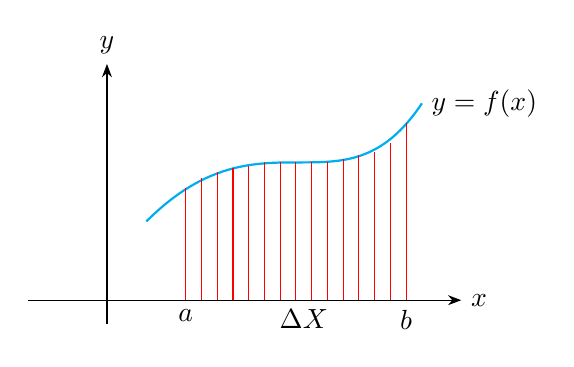
\begin{tikzpicture}[=>stealth]
\draw[-Stealth](-1,0)--(4.5,0)node[right]{$x$};
\draw[-Stealth](0,-0.3)--(0,3)node[above]{$y$};
\draw[thick,cyan](0.5,1)..controls(2,2.5)and (3,1)..(4,2.5);
\draw[red](1,0)--(1,1.43);
\draw[red](3.8,0)--(3.8,2.25);
\draw[red](2.6,0)--(2.6,1.75)
(2.4,0)--(2.4,1.75)
(2.2,0)--(2.2,1.75)
(2,0)--(2,1.75)
(1.8,0)--(1.8,1.7)
(1.6,0)--(1.6,1.68)
(1.4,0)--(1.4,1.63)
(1.2,0)--(1.2,1.55)
(2.8,0)--(2.8,1.75)
(3,0)--(3,1.79)
(3.2,0)--(3.2,1.84)
(3.4,0)--(3.4,1.88)
(3.6,0)--(3.6,2);
\draw(1,0)node[below]{$a$}
(3.8,0)node[below]{$b$}
(4,2.5)node[right]{$y = f(x)$}
(2.5,0)node[below]{$\Delta X$};
\end{tikzpicture}
\end{figure}

\begin{align*}
\text{Area under curve} & = \sum^{\infty}_{i=1} f\big(X_i^*\big)\, \Delta X\\\\
& = \int^b_a f(x)\,dx
\end{align*}
where $f(x)\geq 0$, the Riemann sum can be interpreted as the sum of the areas of the approximating rectangles.


{\color[wave]{485}\subsection{Volumes and Double Integration}}
In a similar manner, we consider a function $f$ of two variables on a closed rectangle

\begin{align*}
R & = [a,b]\times [c,d]\\
& = \big\{(x,y)\in \mathbb{R}^2\hspace{0.1cm}\big|\hspace{0.1cm} a\leq x\leq b\hspace{0.1cm} , \hspace{0.1cm} c \leq y \leq d\big\}
\end{align*}
and suppose $f(x,y)\geq 0$

% DIAGRAM 36
\begin{figure}[H]
\centering
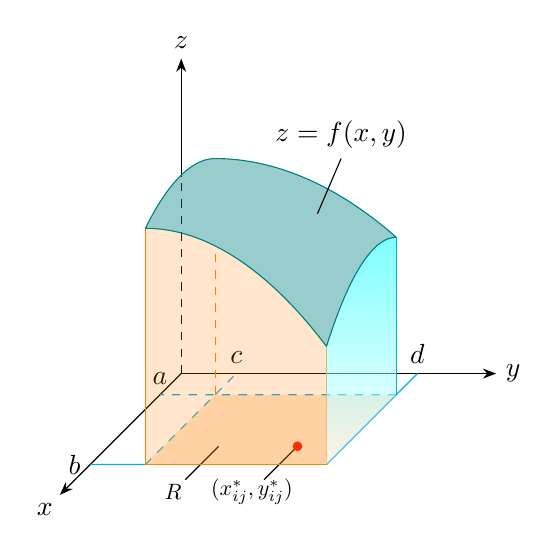
\begin{tikzpicture}[=>stealth]
\draw[-Stealth](0,0,0)--(4,0)node[right]{$y$};
\draw[-Stealth](0,2.5,0)--(0,4,0)node[above]{$z$};
\draw[-Stealth](0,0,0)--(0,0,4);
\draw(0,0,4.5)node[]{$x$};
\draw[dashed](0,0,0)--(0,2.5,0);
%\draw(0.7,0,0.7)--(0.7,0,3)--(3,0,3)--(3,0,0.7)--cycle;
\draw[cyan](0.7,0,3)--(0,0,3)node[left,black]{$b$}
(3,0,3)--(3,0,0)node[above,black]{$d$};
\draw[cyan,dashed](3,0,0.7)--(0,0,0.7)node[above,black]{$a$}
(0.7,0,3)--(0.7,0,0)node[above,black]{$c$};
\draw(2.4,0,2.4)node[shape=circle,fill=red,draw=red,thick,scale=0.01cm]{}
(2.4,0,2.4)--(2.4,0,3.5)
(1.4,0,2.4)--(1.4,0,3.5)
(1.4,0,3.9)node[scale=0.8]{$R$}
(2.4,0,3.9)node[scale=0.8]{$(x_{ij}^*,y_{ij}^*$)};
\draw[orange](0.7,0,3)--(0.7,3,3)
(0.7,0,3)--(3,0,3)
(3,0,3)--(3,1.5,3);
\draw[orange,dashed](0.7,0,0.7)--(0.7,1.8,0.7);
\path[fill=orange,opacity=0.2](0.7,0,0.7)--(0.7,0,3)--(3,0,3)--(3,0,0.7)--cycle;
\path[fill=orange,opacity=0.2](0.7,0,3)--(3,0,3)--(3,1.5,3)parabola[bend at end](0.7,3,3)--(0.7,3,3)--cycle;
\shade[top color=cyan,opacity=0.5](3,0,0.7)--(3,2,0.7)parabola(3,1.5,3)--(3,0,3)--cycle;
\draw[cyan](3,0,0.7)--(3,2,0.7);
\draw[color=teal](3,1.5,3)parabola[bend at end](0.7,3,3)
(3,2,0.7)parabola(3,1.5,3)
(0.7,3,0.7)parabola(3,2,0.7)
(0.7,3,0.7)parabola(0.7,3,3);
\path[fill=teal,opacity=0.4](0.7,3,3)parabola(3,1.5,3)--(3,1.5,3)parabola[bend at end](3,2,0.7)--(3,2,0.7)parabola[bend at end](0.7,3,0.7)--(0.7,3,0.7)parabola(0.7,3,3);
\draw(2,2.3,0.7)--(2.3,3,0.7)node[above]{$z=f(x,y)$};
\end{tikzpicture}
\end{figure}

Let $S$ be the solid that lies above $R$ and under the surface of $f$.
$$\text{i.e}\hspace{0.3cm} S = \big\{(x,y,z)\in \mathbb{R}^3\hspace{0.1cm}\big|\hspace{0.1cm} 0\leq z \leq f(x,y) \in \mathbb{R}^2\big\}$$ 

Our goal is to find the volume of $S$.

%DIAGRAM 37

\begin{figure}[H]
\centering
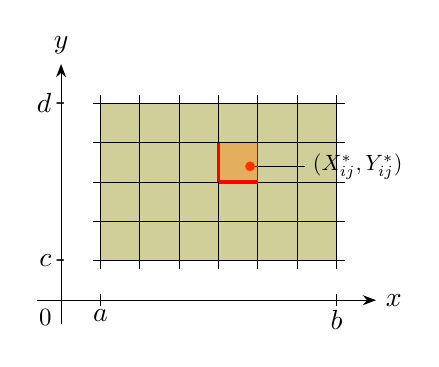
\begin{tikzpicture}[=>stealth]
\draw[-Stealth](-0.3,0)--(4,0)node[right]{$x$};
\draw[-Stealth](0,-0.3)--(0,3)node[above]{$y$};
\draw(0.5,0.5)--(3.5,0.5)--(3.5,2.5)--(0.5,2.5)--cycle;
\path[fill=olive,opacity=0.4](0.5,0.5)--(3.5,0.5)--(3.5,2.5)--(0.5,2.5)--cycle;
\draw[step=0.5cm](0.4,0.4)grid(3.6,2.6);
\draw(0.5,0.08)--(0.5,-0.08)
(3.5,0.08)--(3.5,-0.08)
(0,0.5)node[]{-}
(0,2.5)node[]{-}
(0.5,0)node[below]{$a$}
(3.5,0)node[below]{$b$}
(0,0.5)node[left]{$c$}
(0,2.5)node[left]{$d$}
(2.4,1.7)node[shape=circle,fill=red,draw=red,thick,scale=0.01cm]{}
(2.4,1.7)--(3.1,1.7)node[right,scale=0.8]{$(X_{ij}^*,Y_{ij}^*)$}
(-0.2,0)node[below,scale=0.9]{0};
\path[fill=orange,opacity=0.4](2,1.5)--(2.5,1.5)--(2.5,2)--(2,2)--cycle;
\draw[very thick,red](2,1.5)--(2,2);
\draw[very thick,red](2,1.5)--(2.5,1.5);
\end{tikzpicture}
\end{figure}

We can approximate the part of $S$ that lies above $R_{ij}$ by a thin rectangular box with base $R_{ij}$ and height $f\big(X^*_{ij},Y^*_{ij}\big)$ by $$f\big(X^*_{ij},Y^*_{ij}\big)\Delta A$$

$$V \approx \sum^m_{i=1}\sum^n_{j=1}f\big(X^*_{ij},Y^*_{ij}\big)\Delta A$$


\begin{defn}


The double integral of $f$ over the rectangle $R$ is given by 
$$\iint\limits_R f(x,y)dA = \lim_{m,n\rightarrow \infty}\sum^m_{i=1}\sum^n_{j=1}f\big(X^*_{ij},Y^*_{ij}\big)\Delta A$$ if the limit exist.


If $f(x,y)\geq 0$, then the volume of the solid that lies above $R$ and below the surface $z = f(x,y)$ is $$V = \iint\limits_R f(x,y) dA$$


\end{defn}

\begin{exa}


If $R = \big\{ (x,y)\hspace{0.1cm} \big|\hspace{0.1cm} -\leq x \leq 1 \hspace{0.1cm} , \hspace{0.1cm} -2\leq y\leq 2\big\}$. Evaluate the integral $$\iint\limits_R \sqrt{1 - x^2}\hspace{0.1cm} dA$$
\end{exa}


\begin{solution}


Let $\displaystyle{z = \sqrt{1 - x^2}}\hspace{0.5cm} z\geq 0$


$z^2 + x^2 = 1$

% DIAGRAM 36
\begin{figure}[H]
\centering
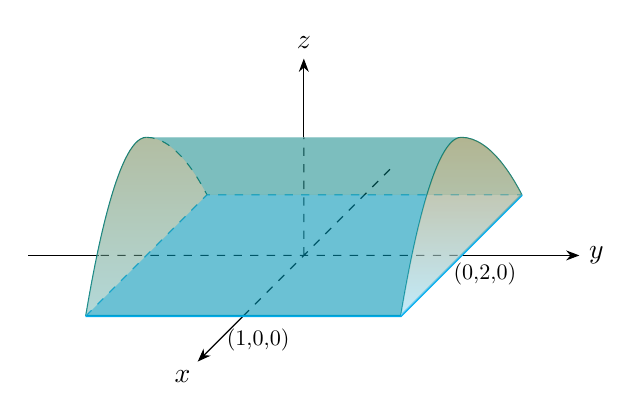
\begin{tikzpicture}[=>stealth]
\draw[-Stealth](2,0,0)--(3.5,0,0)node[right]{$y$};
\draw[-Stealth](0,1.5,0)--(0,2.5,0)node[above]{$z$};
\draw[-Stealth](0,0,2)--(0,0,3.5);
\draw[dashed](-2.58,0,0)--(2,0,0)
(0,0,2)--(0,0,-3)
(0,0,0)--(0,1.5,0);
\draw(0,0,4)node[]{$x$}
(-2.6,0,0)--(-3.5,0,0);
\draw[teal](2,0,2)parabola[bend at end](2,1.5,0)
(2,1.5,0)parabola(2,0,-2)
(-2,1.5,0)parabola(-2,0,2);
\draw[teal,dashed](-2,1.5,0)parabola(-2,0,-2);
\draw[cyan,dashed](-2,0,2)--(-2,0,-2)--(2,0,-2);
\draw[thick,cyan](2,0,-2)--(2,0,2)--(-2,0,2);
\path[fill=cyan,opacity=0.4](-2,0,2)--(-2,0,-2)--(2,0,-2)--(2,0,2)--cycle;
\shade[top color = orange,opacity=0.4](2,0,2)parabola[bend at end](2,1.5,0)--(2,1.5,0)parabola(2,0,-2)--(2,0,-2)--cycle;
\shade[top color=orange,opacity=0.3](-2,0,2)parabola[bend at end](-2,1.5,0)--(-2,1.5,0)parabola(-2,0,-2)--(-2,0,-2)--cycle;
\path[fill = teal,opacity=0.3](2,0,2)parabola[bend at end](2,1.5,0)--(2,1.5,0)--(-2,1.5,0)parabola(-2,0,2)--(-2,0,2)--cycle;
\path[fill = teal,opacity=0.3](2,1.5,0)parabola(2,0,-2)--(2,0,-2)--(-2,0,-2)--(-2,0,-2)parabola[bend at end](-2,1.5,0)--cycle;
\draw(2.3,0)node[below,scale=0.8]{(0,2,0)}
(0,0,2.8)node[right,scale=0.8]{(1,0,0)};
\end{tikzpicture}
\end{figure}

\begin{align*}
V & = \iint\limits_R \sqrt{1 - x^2}\hspace{0.1cm} dA\\
  & = \dfrac{1}{2}\, \pi\, r^2\, h\\\\
  & = \dfrac{1}{2}\, \pi \, (1)\, (4)\\\\
& = 2\pi\\\\
\end{align*}
\end{solution}

{\color[wave]{485}\subsection{Iterated Integrals}}
Suppose that $f$ is a function of two variables that is continuous on the rectangle $R = [a,b]\times [c,d]$.


We use the notation $\displaystyle{\int^d_c(x,y)]\,dy}$ to mean that $x$ is held constant or fixed and $f(x,y)$ is integrated with respect to $y$ from $c$ to $d$ ( partial integration). $$A(x) = \int^d_c f(x,y)\, dy$$
integrating $A(x)$ with respect to $x$ from $a$ to $b$ 
$$\int^b_a A(x)\, dx = \int^b_a \Bigg[\int^d_c f(x,y)\, dy \Bigg] dx$$

$$\int^b_a\int^d_c f(x,y)\,dy\,dx = \int^b_a\Bigg[ \int^d_c f(x,y)\,dy\Bigg] dx\hspace{0.3cm} \cdots\cdots\cdots\cdots\hspace{0.5cm} (1)$$

The integral on the RHS of (1) is called a iterated integral.


Similarly, the iterated integral 
$$\int^d_c\int^b_a f(x,y)\,dx\,dy = \int^d_c\Bigg[ \int^b_a f(x,y)\,dx\Bigg] dy$$


\begin{exa}


Evaluate the iterated integrals $$(a)\hspace{0.5cm} \int^3_0\int^2_1 x^2y\hspace{0.1cm} \,dy\,dx\hspace{2cm} (b)\hspace{0.5cm} \int^2_1\int^3_0 x^2y\,\hspace{0.1cm} dx\,dy$$
\end{exa}


\begin{solution}
\begin{align*}
(a)\hspace{2cm} \int^3_0\int^2_1 x^2y\hspace{0.1cm} \,dy\,dx & = \int^3_0\Bigg[ \int^2_1 x^2y\hspace{0.1cm} \,dy\Bigg]\hspace{0.1cm} \,dx\\\\
& = \int^3_0\frac{3}{2}x^2\hspace{0.1cm}\, dx\\\\
& = \frac{27}{2}\\
\end{align*}

\begin{align*}
 \hspace{2cm} \int^2_1\int^3_0 x^2y\hspace{0.1cm}\, dx\, dy & =  \int^2_1\Bigg[ \int^3_0 x^2y\,\hspace{0.1cm}\, dx\Bigg] dy\\\\
 &  = \int^2_1 9y\hspace{0.1cm}\, dy\\\\
 & = \frac{27}{2}\\\\
\end{align*}
\end{solution}

\subhead{Fubini's Theorem}


If $f$ is continuous on the rectangle \hspace{0.2cm}$R = \big\{ (x,y)\hspace{0.1cm} \big|\hspace{0.1cm} a\leq x \leq b\hspace{0.1cm} , \hspace{0.1cm} c\leq y\leq d\big\}\hspace{0.2cm}$ then 
\begin{align*}
\iint\limits_R f(x,y)\hspace{0.1cm} dA & = \int^b_a \int^d_c f(x,y)\hspace{0.1cm}dy\hspace{0.1cm} dx\\\\
& = \int^d_c \int^b_a f(x,y)\hspace{0.1cm}dx\hspace{0.1cm} dy\\\\
\end{align*}

\begin{exa}


Evaluate the double $\displaystyle{\iint\limits_R \big(x-3y^2\big)\hspace{0.1cm}dA}$ $$R = \big\{ (x,y)\hspace{0.1cm} \big|\hspace{0.1cm} 0\leq x \leq 2\hspace{0.1cm} , \hspace{0.1cm} 1 \leq y \leq y \big\}$$
\end{exa}


\begin{solution}
\begin{align*}
\iint\limits_R \big(x-3y^2\big)\hspace{0.1cm}dA & = \int^2_0\int^2_1 \big(x-3y^2\big)\hspace{0.1cm} dy \hspace{0.1cm} dx\\
& = \int^2_0 (x - 7)\hspace{0.1cm}dx\\
& = -12\\
\end{align*}

\begin{align*}
\int^2_1\int^2_0 \big(x-3y^2\big)\hspace{0.1cm} dx \hspace{0.1cm} dy & = \int^2_1 \big(2 - 6y^2\big)\hspace{0.1cm} dy\\
& = -12\\\\
\end{align*}
\end{solution}

\begin{exa}


Evaluate $\displaystyle{\iint\limits_R y \sin (xy)\hspace{0.1cm}dA}$ where $R = [1,2]\times [0,\pi]$
\end{exa}


\begin{solution}
\begin{align*}
\iint\limits_R y \sin (xy) \hspace{0.1cm} dA & = \int^{\pi}_0 \int^2_1 y\sin (xy) \hspace{0.1cm}dx\hspace{0.1cm} dy\\
& = \int^{\pi}_0 \big(-\cos 2y + \cos y\big)\hspace{0.1cm} dy\\
& = 0\\
\end{align*}
\end{solution}

\begin{solution}
\begin{align*}
\iint\limits_R y \sin (xy) \hspace{0.1cm} dA & = \int^2_1 \int^{\pi}_0 y\sin (xy) \hspace{0.1cm}dy\hspace{0.1cm} dx\\\\
& =\int^2_1 \Bigg( \frac{-\pi \cos \pi x}{x} + \frac{\sin \pi x}{x^2}\Bigg) \hspace{0.1cm}dx
\end{align*}
Let $u = \dfrac{-1}{x} \implies du = \dfrac{dx}{x^2}$


$dv = \pi \cos \pi x \implies v = \sin \pi x$


$$\int \frac{\pi \cos \pi x}{x}dx = \frac{- \sin \pi x}{x} - \int \frac{\sin \pi x}{x^2}dx$$

\begin{align*}
\int^2_1 \Bigg( \frac{-\pi \cos \pi x}{x} + \frac{\sin \pi x}{x^2}\Bigg) & = \frac{-\sin \pi x}{x}\Bigg|^2_1\\
& = 0\\\\
\end{align*}
\end{solution}

\begin{exa}


Find the volume of the solid $S$ that is bounded by the elliptic parababloid $$x^2+ 2y^2 + z = 16$$ the planes $x=2, y = 2$ and the three coordinate planes.

% DIAGRAM 39

\begin{figure}[H]
\centering
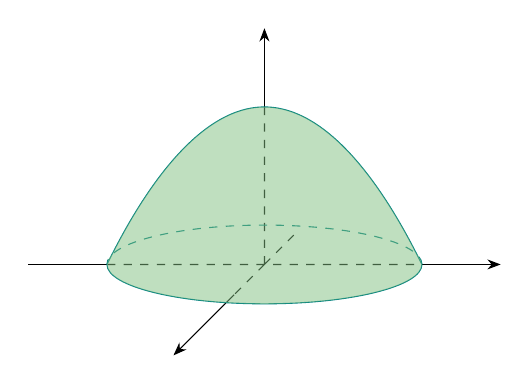
\begin{tikzpicture}[=>stealth]
\draw[dashed](-2,0,0)--(2,0,0)
(0,0,0)--(0,2,0)
(0,0,0)--(0,0,1)
(0,0,0)--(0,0,-1);
\draw[-Stealth](0,2,0)--(0,3,0);
\draw[-Stealth](2,0,0)--(3,0,0);
\draw[-Stealth](0,0,1)--(0,0,3);
\draw(-3,0,0)--(-2,0,0);
\draw[teal](0,2)parabola(2,0)
(0,2)parabola(-2,0);
\draw[teal](-2,0)arc(180:360:2cm and 0.5cm);
\draw[dashed,teal](2,0)arc(0:180:2cm and 0.5cm);
\path[fill=orange!50!cyan,opacity=0.5](0,0)circle(2cm and 0.5cm)--(2,0)parabola[bend at end](0,2)--(0,2)parabola(-2,0);
\end{tikzpicture}
\end{figure}
\end{exa}

\begin{solution}


We note that the solid $S$ lies under the surface $z = 16 - x^2 -2y^2$ and above the square $R = [0,2]\times [0,2]$.
\begin{align*}
V & = \iint\limits_R \big( 16 - x^2 - 2y^2\big)\hspace{0.1cm} dA\\
& = \int^2_0\int^2_0 \big(16 - x^2 -2y^2 \big) \hspace{0.1cm}dx\hspace{0.1cm} dy\\
& = \int^2_0\Bigg( \frac{88}{3} - 4y^2\Bigg)\hspace{0.1cm}dy\\
& = 48\\
\end{align*}

In the special case where $f(x,y)$ can be factored as the product of a function of $x$ only and a function of $y$, then the double integral as follows:-


Suppose $f(x,y) = g(x)h(x)\hspace{0.5cm}, \hspace{0.5cm} R = [a,b]\times [a,b]$

$$ \iint\limits_R f(x,y)\hspace{0.1cm}dA = \int^b_ag(x)\,dx\int^b_ah(y)\,dy$$
\end{solution}


\begin{exa}


Evaluate $\displaystyle{\iint\limits_R \sin x \cos y \hspace{0.1cm} dy\hspace{0.1cm}dx}$ where $R = \big[ 0,\pi/2\big] \times \big[ 0,\pi/2\big]$.
\end{exa}


\begin{solution}


$\displaystyle{\iint\limits_R \sin x \cos y \hspace{0.1cm} dy\hspace{0.1cm}dx    = \int^{\pi/2}_0 \sin x \hspace{0.1cm} dx \int^{\pi/2}_0\cos y \hspace{0.1cm}dy\\
= 1}$
\end{solution}


{\color[wave]{485}\subsection{Double Integrals Over General Regions}}
Suppose that $D$ is a bounded region then $D$ can be enclosed in a rectangular region.


We define a new function $F(x,y)$ with domain $R$.

\[ F(x,y) = 
\begin{cases}
f(x,y) , & \text{If}\hspace{0.2cm} (x,y)\in D\\\\
0 , & \text{If} \hspace{0.2cm} (x,y)\not\in D\\
\end{cases}
\]

If the double integral exist over $R$, then we define the double integral of $f$ over $D$ by $$\iint\limits_D f(x,y)\hspace{0.1cm}dA = \iint\limits_R F(x,y)\hspace{0.1cm}dA$$

A plane region $D$ is said to be \textit{type I} if it lies between the graphs of two continuous functions of $x$ $$ D = \big\{ (x,y)\hspace{0.1cm} \big|\hspace{0.1cm} a \leq x \leq b \hspace{0.1cm} , \hspace{0.1cm} g_1(x) \leq y\leq g_2(x)\big\}$$ where $g_1(x)$ and $g_2(x)$ are continuous on $[a,b]$.

% DIAGRAM 40

\begin{table}[H]
\centering
\begin{tabular}{ccccccccc}
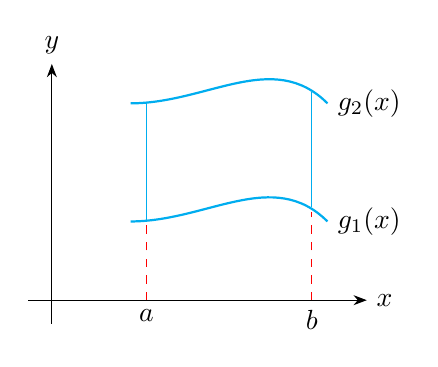
\begin{tikzpicture}[=>stealth]
\draw[-Stealth](-0.3,0)--(4,0)node[right]{$x$};
\draw[-Stealth](0,-0.3)--(0,3)node[above]{$y$};
\draw[cyan,thick,out=0](1,1)to(3.5,1)node[right,black]{$g_1(x)$};
\draw[cyan,thick,out=0](1,2.5)to(3.5,2.5)node[right,black]{$g_2(x)$};
\draw[cyan](1.2,1.02)--(1.2,2.5)
(3.3,1.18)--(3.3,2.65);
\draw[dashed,red](1.2,0)--(1.2,1)
(3.3,0)--(3.3,1.12);
\draw(1.2,0)node[below]{$a$}
(3.3,0)node[below]{$b$};
\end{tikzpicture}
&&&&&&&&
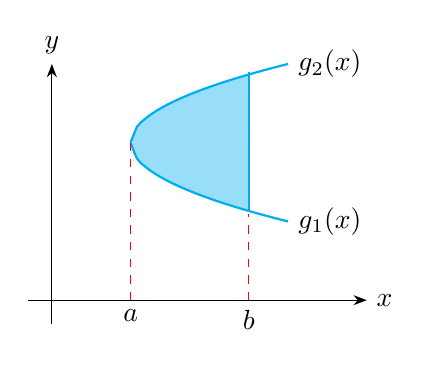
\begin{tikzpicture}[=>stealth]
\draw[-Stealth](-0.3,0)--(4,0)node[right]{$x$};
\draw[-Stealth](0,-0.3)--(0,3)node[above]{$y$};
\draw[smooth,domain=1:3,variable=\x,thick,cyan]plot(\x,{2+1/2*sqrt(2*(\x-1))})node[right,black]{$g_2(x)$};
\draw[smooth,domain=1:3,variable=\x,thick,cyan]plot(\x,{2-1/2*sqrt(2*(\x-1))})node[right,black]{$g_1(x)$};
\draw[dashed,red](1,0)--(1,2)
(2.5,0)--(2.5,1.1);
\draw[thick,cyan](2.5,1.15)--(2.5,2.9);
\draw(1,0)node[below]{$a$}
(2.5,0)node[below]{$b$};
\path[fill=cyan,opacity=0.4,domain=1:2.5,variable=\x]plot(\x,{2+1/2*sqrt(2*(\x-1))})--(2.5,2.9)--(2.5,2.001)--(1,2)--cycle;
\path[fill=cyan,opacity=0.4,domain=1:2.5,variable=\x]plot(\x,{2-1/2*sqrt(2*(\x-1))})--(2.5,1.16)--(2.5,2)--(1,2)--cycle;
\end{tikzpicture}\\
\end{tabular}
\end{table}

% DIAGRAM 41

\begin{figure}[H]
\centering
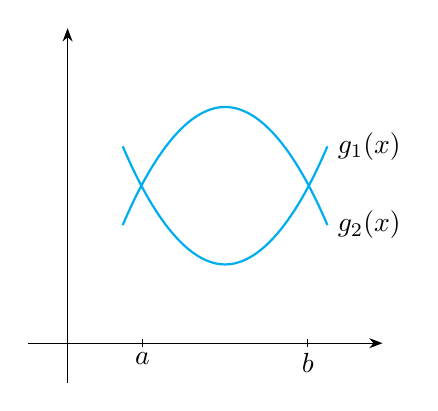
\begin{tikzpicture}[=>stealth]
\draw[-Stealth](-0.5,0)--(4,0);
\draw[-Stealth](0,-0.5)--(0,4);
\draw[thick,cyan](2,1)parabola(3.3,2.5)node[right,black]{$g_1(x)$}
(2,1)parabola(0.7,2.5)
(2,3)parabola(3.3,1.5)node[right,black]{$g_2(x)$}
(2,3)parabola(0.7,1.5);
\draw(0.95,0)node[below]{$a$}
(3.05,0)node[below]{$b$};
\draw(3.05,-0.05)--(3.05,0.05)
(0.95,-0.05)--(0.95,0.05);
\end{tikzpicture}
\end{figure}

 To evaluate $\displaystyle{\iint\limits_D f(x,y)\hspace{0.1cm}dA}$ when $D$ is a \textit{type I} region, we choose rectangle $R = [a,b] \times [c,d]$ that contains $D$.

% DIAGRAM 42

\begin{figure}[H]
\centering
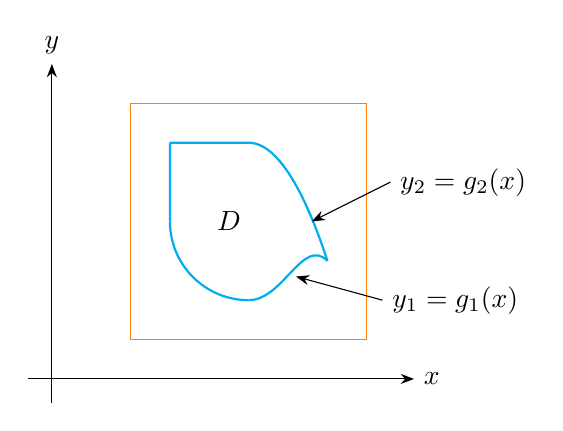
\begin{tikzpicture}[=Stealth]
\draw[-Stealth](-0.3,0)--(4.6,0)node[right]{$x$};
\draw[-Stealth](0,-0.3)--(0,4)node[above]{$y$};
\draw[thick,cyan](1.5,2)arc[start angle=180, end angle=270, radius=1cm];
\draw[thick,cyan](1.5,3)--(2.5,3)
(2.5,3)parabola(3.5,1.5)
(1.5,3)--(1.5,2);
\draw[thick,cyan,out=0](2.5,1)to(3.5,1.5);
\draw(2.25,2)node[]{$D$}
(4.3,2.5)node[right]{$y_2=g_2(x)$}
(4.2,1)node[right]{$y_1=g_1(x)$};
\draw[orange](1,0.5)--(4,0.5)--(4,3.5)--(1,3.5)--cycle;
\draw[-Stealth](4.3,2.5)--(3.3,2);
\draw[-Stealth](4.2,1)--(3.1,1.3);
\end{tikzpicture}
\end{figure}

\begin{align*}
\iint\limits_D f(x,y)\hspace{0.1cm} dA & = \iint\limits_R F(x,y)\hspace{0.1cm}dA\\
& = \int^b_a\int^d_c F(x,y)\hspace{0.1cm} dy \hspace{0.1cm}dx\\
\end{align*} 

Note $F(x,y) = 0 \hspace{0.4cm} y<g_1(x) \hspace{0.2cm} , \hspace{0.2cm} y>g_2(x)$
\begin{align*}
\int^d_c F(x,y)\hspace{0.1cm}dy & = \int^{g_2(x)}_{g_1(x)} F(x,y)\hspace{0.1cm}dy\\
& = \int^{g_2(x)}_{g_1(x)} f(x,y)\hspace{0.1cm}dy\\
\end{align*} 

because $F(x,y) = f(x,y)$ when $g_1(x) \leq y \leq g_2(x)$. If $f$ is continuous on $\textit{type I}$ region $D$ such that \hspace{0.2cm}$D = \big\{ (x,y)\hspace{0.1cm} \big|\hspace{0.1cm} a\leq x \leq b \hspace{0.1cm} , \hspace{0.1cm} g_1(x)\leq y\leq g_2(x)\big\}\hspace{0.2cm}$ then $$\iint\limits_D f(x,y)\hspace{0.1cm}dA = \int^b_a\int^{g_2(x)}_{g_1(x)} f(x,y)\hspace{0.1cm}dy\hspace{0.1cm}dx$$


Consider plane regions of $\textit{type II}$ which can be expressed as 
$$D = \big\{ (x,y)\hspace{0.1cm} \big|\hspace{0.1cm} c\leq x \leq d \hspace{0.1cm} , \hspace{0.1cm} h_1(x)\leq y\leq h_2(x)\big\}$$
Where $h_1$ and $h_2$ are continuous
 $$\iint\limits_D f(x,y)\hspace{0.1cm}dA = \int^d_c\int^{h_2(x)}_{h_1(x)} f(x,y)\hspace{0.1cm}dx\hspace{0.1cm}dy$$

% DIAGRAM 43

\begin{table}[H]
\centering
\begin{tabular}{cccccc}
\begin{tikzpicture}[=>stealth]
\draw[-Stealth](-0.3,0)--(4,0)node[right]{$x$};
\draw[-Stealth](0,-0.3)--(0,4)node[above]{$y$};
\draw[cyan](1,1)--(3.5,1)
(1,2.5)--(3.5,2.5);
\draw[thick,cyan,out=0](1,1)to(1,2.5);
\draw[thick,cyan,out=0](3.5,1)to(3.5,2.5);
\draw[dashed,red](1,1)--(0,1)
(1,2.5)--(0,2.5);
\draw(0,1)node[left]{$c$}
(0,2.5)node[left]{$d$}
(3.5,1.75)node[right]{$h_2(y)$}
(1.2,1.75)node[left]{$h_1(y)$};
\end{tikzpicture}
&&&&&
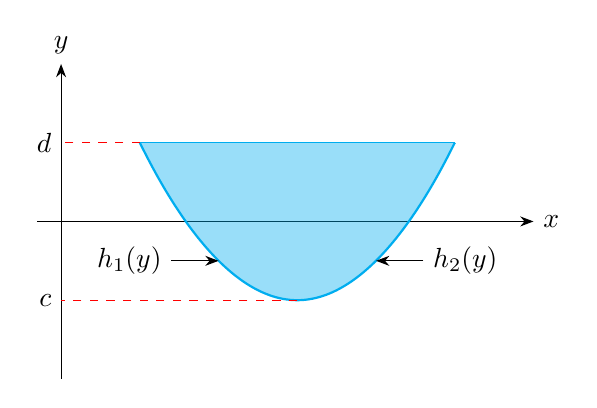
\begin{tikzpicture}[=>stealth]
\draw[-Stealth](-0.3,0)--(6,0)node[right]{$x$};
\draw[-Stealth](0,-2)--(0,2)node[above]{$y$};
\draw[thick,cyan](3,-1)parabola(1,1)
(3,-1)parabola(5,1);
\path[fill=cyan,opacity=0.4](5,1)parabola[bend at end](3,-1)--(3,-1)parabola(1,1)--(1,1)--(5,1)--cycle;
\draw[cyan](1,1)--(5,1);
\draw[red,dashed](3,-1)--(0,-1)
(1,1)--(0,1);
\draw(0,1)node[left]{$d$}
(0,-1)node[left]{$c$}
(4.6,-0.5)node[right]{$h_2(y)$}
(1.4,-0.5)node[left]{$h_1(y)$};
\draw[-Stealth](4.6,-0.5)--(4,-0.5);
\draw[-Stealth](1.4,-0.5)--(2,-0.5);
\end{tikzpicture}
\end{tabular}
\end{table}

\vspace{1cm}

\begin{exa}


Evaluate $\displaystyle{\iint\limits_D  (x + 2y)\hspace{0.1cm}dA}$ where $D$ is the region bounded by the parabolas $y = 2x^2$ and $y = 1 + x^2$.

% DIAGRAM 44

\begin{figure}[H]
\centering
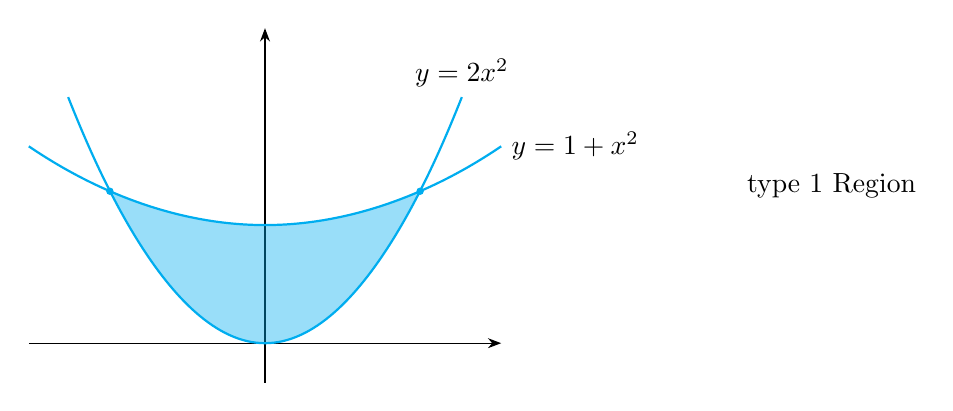
\begin{tikzpicture}[=>stealth]
\draw[-Stealth](-3,0)--(3,0);
\draw[-Stealth](0,-0.5)--(0,4);
\draw[thick,cyan](0,0)parabola(2.5,3.125)node[above,black]{$y=2x^2$}
(0,0)parabola(-2.5,3.125);
\draw[thick,cyan](0,1.5)parabola(3,2.5)node[right,black]{$y = 1 + x^2$}
(0,1.5)parabola(-3,2.5);
\draw(1.97,1.93)node[shape=circle,fill=cyan,scale=0.01cm]{}
(-1.97,1.93)node[shape=circle,fill=cyan,scale=0.01cm]{}
(6,2)node[right]{type 1 Region};
\path[fill=cyan,opacity=0.4](0,0)parabola(1.97,1.93)--(1.97,1.93)parabola[bend at end](0,1.5)--(0,1.5)parabola(-1.97,1.93)--(-1.97,1.93)parabola[bend at end](0,0)--cycle;
\end{tikzpicture}
\end{figure}

\begin{align*}
\iint\limits_D  (x + 2y)\hspace{0.1cm}dA & = \int^1_{-1}\int^{1 + x^2}_{2x^2} \big(x + 2y\big)\hspace{0.1cm}dy\hspace{0.1cm}\\
& = \int^1_{-1}\big(-3x^4 - x^3 +  2x^2 + x + 1\big)\hspace{0.1cm}dx\\\\
& = \frac{32}{5}\\\\
\end{align*}
\end{exa}

\begin{exa}


Find the volume of the solid that has under the paraboloid $z = x^2 + y^2$ and above the region $D$ in the $xy-$plane bounded by the line $y = 2x$ and the parabola $y = x^2$.

% DIAGRAM 45

\begin{figure}[H]
\centering
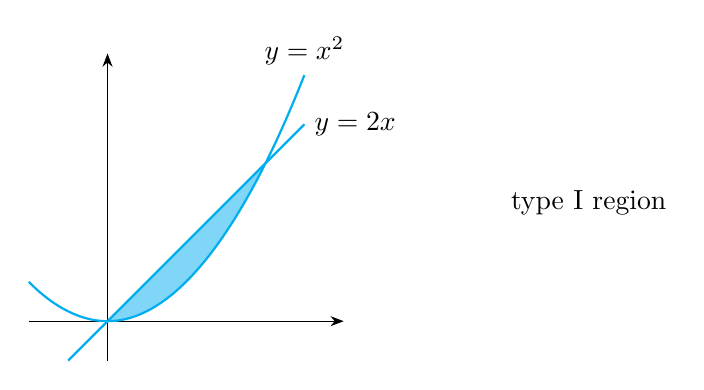
\begin{tikzpicture}[=>stealth]
\draw[-Stealth](-1,0)--(3,0);
\draw[-Stealth](0,-0.5)--(0,3.4);
\draw[thick,cyan](0,0)parabola(2.5,3.125)node[above,black]{$y=x^2$};
\draw[thick,cyan](0,0)parabola(-1,0.5);
\draw[thick,cyan](-0.5,-0.5)--(2.5,2.5)node[right,black]{$y=2x$};
\draw(5,1.5)node[right]{type I region};
\path[fill=cyan,opacity=0.5](0,0)parabola(2,2)--(0,0)--cycle;
\end{tikzpicture}
\end{figure}

$$D = \big\{ (x,y)\hspace{0.1cm}\big|\hspace{0.1cm} 0 \leq x\leq 2\hspace{0.1cm} , \hspace{0.1cm} x^2 \leq y \leq 2x\big\}$$

Therefore the volume under $z = x^2 + y^2$ and above $D$.

\begin{align*}
V & = \iint\limits_D \big(x^2+y^2\big)\hspace{0.1cm}dA\\
& = \int^2_0\int^{2x}_{x^2}\big(x^2 + y^2\big)\hspace{0.1cm}dy \hspace{0.1cm}dx\\
& = \int^2_0\Bigg( \frac{-x^6}{3} -x^4 +\frac{14 x^3}{3}\Bigg)\hspace{0.1cm} dx\\\\
& = \frac{216}{35}\\\\
\end{align*}

% DIAGRAM 46

\begin{figure}[H]
\centering
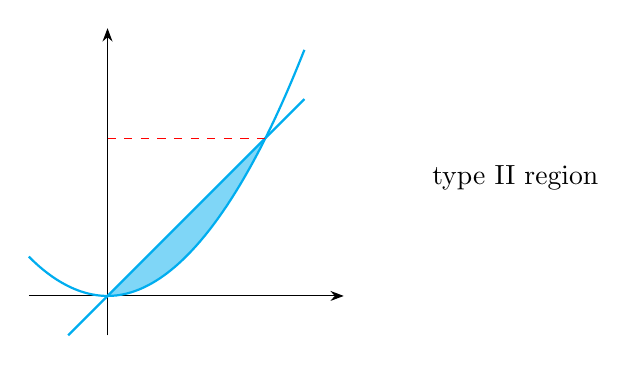
\begin{tikzpicture}[=>stealth]
\draw[-Stealth](-1,0)--(3,0);
\draw[-Stealth](0,-0.5)--(0,3.4);
\draw[thick,cyan](0,0)parabola(2.5,3.125);
\draw[thick,cyan](0,0)parabola(-1,0.5);
\draw[thick,cyan](-0.5,-0.5)--(2.5,2.5);
\draw[dashed,red](0,2)--(2,2);
\draw(4,1.5)node[right]{type II region};
\path[fill=cyan,opacity=0.5](0,0)parabola(2,2)--(0,0)--cycle;
\end{tikzpicture}
\end{figure}

$$y = 2x \implies x = \frac{y}{2}$$

$$y = x^2 \implies x = \pm \sqrt{y}$$

$$D = \big\{(x,y)\hspace{0.1cm}\big|\hspace{0.1cm} 0\leq y\leq 4\hspace{0.1cm},\hspace{0.1cm} y/2\leq x \leq \sqrt{y}\big\}$$

\begin{align*}
V & = \iint\limits_D \big(x^2+y^2\big)\hspace{0.1cm}dA\\
& = \int^4_0\int^{\sqrt{y}}_{y/2}\big(x^2 + y^2\big)\hspace{0.1cm}dx \hspace{0.1cm}dy\\
& = \int^4_0\Bigg(\frac{y^{3/2}}{3} + y^{5/2} - \frac{y^3}{24} - \frac{y^3}{2}\Bigg)\hspace{0.1cm} dy\\\\
& = \frac{216}{35}\\\\
\end{align*}
\end{exa}

\begin{exa}


Evaluate $\displaystyle{\iint\limits_D xy\hspace{0.1cm}dA}$ where $D$ is the region bounded by $y = x -1$ and $y^2 = 2x + 6$.

% DIAGRAM 47

\begin{figure}[H]
\centering
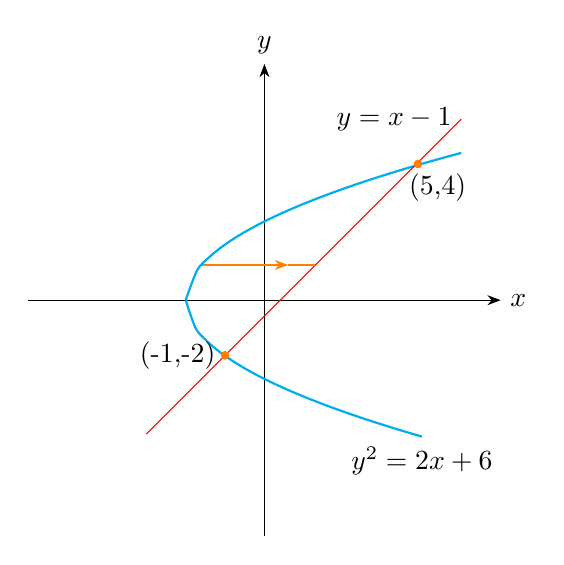
\begin{tikzpicture}[=>stealth]
\draw[-Stealth](-3,0)--(3,0)node[right]{$x$};
\draw[-Stealth](0,-3)--(0,3)node[above]{$y$};
\draw[-Stealth,orange](-0.8,0.447)--(0.3,0.447);
\draw[smooth,domain=-1:2.5,variable=\x,thick, cyan]plot(\x,{sqrt(\x+1)});
\draw[smooth,domain=-1:2,variable=\x,thick,cyan]plot(\x,{-sqrt(\x+1)})node[below,black]{$y^2 = 2x + 6$};
\draw[smooth,domain=-1.5:2.5,variable=\x,red]plot(\x,\x-0.2)node[left,black]{$y = x - 1$};
\draw[orange](0.3,0.447)--(0.647,0.447);
\draw(-0.5,-0.7)node[shape=circle,draw=orange,fill=orange,scale=0.01cm]{}
(1.95,1.73)node[shape=circle,draw=orange,fill=orange,scale=0.01cm]{}
(2.2,1.73)node[below]{(5,4)}
(-0.5,-0.7)node[left]{(-1,-2)};
\end{tikzpicture}
\end{figure}

\begin{enumerate}
\item[]
\begin{enumerate}
       \item $D$ as type I 

       \item $D$ as type II region.
\end{enumerate}
\end{enumerate}
\end{exa}

\begin{solution}
\begin{align*}
(b)\hspace{2cm} \iint\limits_D xy\hspace{0.1cm} dA & = \int^4_{-2}\int^{y+1}_{1/2(y^2-6)}xy\hspace{0.1cm}dx\,dy\\
& = \int^4_{-2}\Bigg(\frac{-y^5}{4} + 4y^3 + 2y^2 - 8y\Bigg) \hspace{0.1cm}dy\\
& = 36\\
\end{align*}

$(a)\hspace{0.6cm}$ NB If $D$ is taken as \textit{type I}, then 
\begin{align*}
\iint\limits_D xy\hspace{0.1cm} dA = \int^{-1}_{-3}\int^{\sqrt{2x + 6}}_{-\sqrt{2x + 6}}xy \hspace{0.1cm}dx\,dy +  \int^{5}_{-1}\int^{y=\sqrt{2x + 6}}_{y = x -1}xy \hspace{0.1cm}dy\,dx\\\\ 
\end{align*}
\end{solution}

\begin{exa}


Find the volume of the tetrahedron bounded by the planes $x + 2y + z = 2.$


$x = 2y\hspace{0.3cm} , \hspace{0.3cm} x = 0\hspace{0.3cm} , \hspace{0.3cm} z = 0$

%DIAGRAM 48

\begin{figure}[H]
\centering
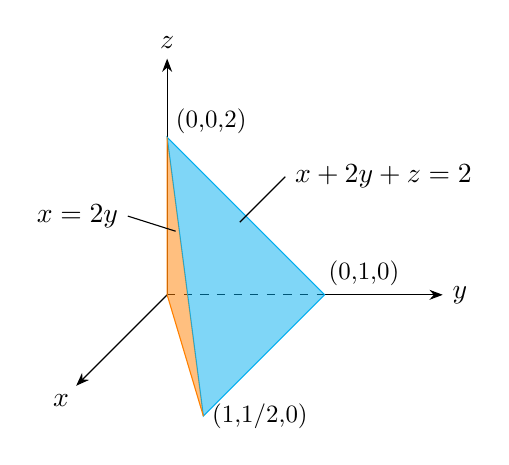
\begin{tikzpicture}[=>stealth]
\draw[-Stealth](2,0,0)--(3.5,0,0)node[right]{$y$};
\draw[-Stealth](0,0,0)--(0,3,0)node[above]{$z$};
\draw[-Stealth](0,0,0)--(0,0,3);
\draw[dashed](0,0,0)--(2,0,0);
\path[fill=cyan,opacity=0.5](2,0,4)--(2,0,0)--(0,2,0)--cycle;
\draw[cyan](2,0,4)--(2,0,0)--(0,2,0)--cycle;
\path[fill=orange,opacity=0.5](2,0,4)--(0,2,0)--(0,0,0)--cycle;
\draw[orange](2,0,4)--(0,0,0)--(0,2,0);
\draw(2,0,4)node[right,scale=0.9]{(1,1/2,0)}
(0,2.2,0)node[right,scale=0.9]{(0,0,2)}
(2.5,0,0)node[above,scale=0.9]{(0,1,0)}
(0,0,3.5)node[]{$x$};
\draw(1,1,0.2)--(1.5,1.5,0)node[right]{$x + 2y + z = 2$}
(0.3,1,0.5)--(-0.5,1,0)node[left]{$x = 2y$};
\end{tikzpicture}
\end{figure}
\vspace{1cm}

% DIAGRAM 49

\begin{figure}[H]
\centering
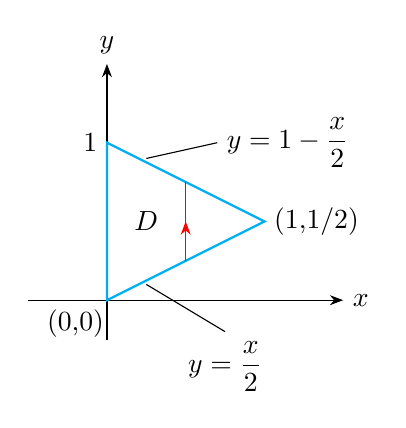
\begin{tikzpicture}[=>stealth]
\draw[-Stealth](-1,0)--(3,0)node[right]{$x$};
\draw[-Stealth](0,-0.5)--(0,3)node[above]{$y$};
\draw[thick,cyan](0,0)--(2,1)--(0,2)--cycle;
\draw(0,2)node[left]{1}
(-0.4,0)node[below]{(0,0)}
(2,1)node[right]{(1,1/2)}
(0.5,1)node[]{$D$};
\draw[red](1,0.5)--(1,1.5);
\draw[red,-Stealth](1,0.5)--(1,1);
\draw(0.5,1.8)--(1.4,2)node[right]{$y = 1 - \dfrac{x}{2}$};
\draw(0.5,0.2)--(1.5,-0.4)node[below]{$y = \dfrac{x}{2}$};
\end{tikzpicture}
\end{figure}

The required volume lies under the graph $z = 2 - x - 2y$ and above $$D = \Big\{(x,y)\hspace{0.1cm}:\hspace{0.1cm} 0\leq x\leq 1\hspace{0.1cm} ,\hspace{0.1cm} \dfrac{x}{2}\leq y \leq 1 - \frac{x}{2}\Big\}$$

\begin{align*}
V & = \iint\limits_D \big( 2 - x -2y\big)\hspace{0.1cm}dA\\
& = \int^1_0\int^{1 -x/2}_{x/2} \big( 2 - x -2y\big)\hspace{0.1cm}dy\,dx\\
& = \int^1_0\big(x^2 - 2x + 1\big)\hspace{0.1cm}dx
  = \frac{1}{3}\\\\
\end{align*}
\end{exa}

\begin{exa}


Evaluate the iterated integral $\displaystyle{\int^1_0\int^1_{x}\sin (y^2)\hspace{0.1cm}dy\,dx}$

% DIAGRAM 49
\begin{figure}[H]
\centering
\begin{tikzpicture}[=>stealth]
\draw[-Stealth](-1,0)--(3,0);
\draw[-Stealth](0,-0.5)--(0,3);
\draw[cyan](0,0)--(2.5,2.5)node[above,black]{$y = x$}
(0,2)--(2.5,2)node[right,black]{$y=1$};
\path[fill=cyan,opacity=0.3](0,0)--(2,2)--(0,2)--cycle;
\draw(0,2)node[left]{1}
(2,0)node[below]{1}
(-0.2,0)node[below]{0}
(-2,1)node[left]{(a).}
(6.5,1)node[left]{(b).}
(10,2)node[shape=circle,fill=cyan,scale=0.01cm]{}
(10.2,2)node[below,scale=0.9]{(1,1)};
\draw[dashed,red](2,0)--(2,2);
\draw[-Stealth,red](1,1)--(1,2);
\draw[-Stealth](7.5,0)--(11,0);
\draw[-Stealth](8,-0.5)--(8,3);
\draw[red,-Stealth](8,1)--(8.5,1);
\draw[cyan](8,0)--(10.5,2.5)
(8,2)--(10.5,2);
\path[fill=cyan,opacity=0.3](8,0)--(8,2)--(10,2)--cycle;
\draw[red](8,1)--(9,1);
\end{tikzpicture}
\end{figure}

\begin{align*}
\int^1_0\int^y_{0}\sin (y^2)\hspace{0.1cm}dx\,dy & = \int^1_0y\sin (y^2)\hspace{0.1cm}dy\\
& = \frac{1}{2}\big(1 - \cos(1)\big)\\\\\\
\end{align*}
\end{exa}

{\color[wave]{485}\subsection{Properties Of Double Integrals}}
\begin{enumerate}
\item $\displaystyle{\iint\limits_D \big(f(x,y) + g(x,y)\big)\hspace{0.1cm}dA = \iint\limits_D f(x,y)\hspace{0.1cm}dA   +   \iint\limits_D g(x,y)\hspace{0.1cm}dA}$

\item $\displaystyle{ \iint\limits_D C\hspace{0.1cm} f(x,y)\hspace{0.1cm}dA  = C \iint\limits_D f(x,y)\hspace{0.1cm}dA }$

\item If $f(x,y)\geq g(x,y)$ for all $(x,y)\in D$ then $\displaystyle{\iint\limits_D f(x,y)\hspace{0.1cm}dA \geq \iint\limits_D g(x,y)\hspace{0.1cm}dA }$.
\item If $D = D_1\cup D_2$ where $D_1$ and $D_2$ do not overlap except perhaps on the boundary $$\iint\limits_D f(x,y)\hspace{0.1cm}dA  = \iint\limits_{D_1} f(x,y)\hspace{0.1cm}dA  + \iint\limits_{D_2} f(x,y)\hspace{0.1cm}dA $$
\item If we integrate the constant function $f(x,y) = 1$ over a region $D$ we get the area of $D$ $$\iint\limits_D 1 \hspace{0.1cm}dA = A(D)$$
\item If $m\leq f(x,y) \leq M$ for all $(x,y) \in D$ then $$m\hspace{0.1cm}A(D)\leq \iint\limits_D f(x,y)\hspace{0.1cm}dA \leq M\hspace{0.1cm} A(D)$$
\end{enumerate}

\begin{exa}


Use property 6 to estimate the integral $\displaystyle{\iint\limits_De^{\displaystyle{\sin x \cos y}}\hspace{0.1cm} dA}$ where $dA$ is the disk with centre origin and radius 2.
\end{exa}


\begin{solution}
\begin{align*}
\text{Since}\hspace{1cm} -1 & \leq \sin x \leq 1\\
-1 & \leq \cos y \leq 1 \hspace{1cm} \implies -1 \leq \sin x \cos y\leq 1
\end{align*}

\begin{align*}
e^{-1} & \leq e^{\displaystyle{\sin x \cos y}} \leq e^1\\
\frac{1}{e} & \leq e^{\displaystyle{\sin x \cos y}} \leq e\\
\end{align*}

Using $m = \dfrac{1}{e}$ and $M = e$


Area of disc $= \pi (2)^2 = 4\pi$

$$\therefore \hspace{0.4cm} \frac{4\pi}{e}\leq \iint\limits_D e^{\displaystyle{\sin x \cos y}}\hspace{0.1cm} dA \leq 4\pi e$$
\end{solution}


{\color[wave]{485}\subsection{Double Integrals In Polar Coordinates}}
Suppose that we want to integrate $\displaystyle{\iint\limits_R f(x,y)\hspace{0.1cm}dA}$ where $R$ is one of the regions shown below.

% DIAGRAM 50

\begin{figure}[H]
\centering
\begin{tikzpicture}[=>stealth]
\draw[-Stealth](-2,0)--(2,0);
\draw[-Stealth](0,-2)--(0,2);
\draw[thick,cyan](0,0)circle[radius=1.5cm];
\path[fill=cyan,opacity=0.4](0,0)circle[radius=1.5cm];
\draw(0.5,0.5)node[]{$R$};
\draw(1,1.2)--(1.5,1.4)node[above]{$x^2 + y^2 = 1$};
\draw[-Stealth](5.5,0)--(10.5,0);
\draw[-Stealth](8,-1)--(8,2.5);
\draw[thick,cyan](9,0)arc[start angle = 0, end angle=180, radius=1];
\draw[thick,cyan](10,0)arc[start angle = 0, end angle = 180, radius =2];
\draw[thick,cyan](6,0)--(7,0)
(9,0)--(10,0);
\draw(9,1)node[above]{$R$}
(-2,1)node[left]{a.}
(5.5,1)node[left]{b.};
\path[fill=cyan,opacity=0.4](9,0)arc[start angle=0,end angle = 180,radius=1]--(7,0)--(6,0)--(6,0)arc[start angle=180, end angle = 0, radius=2]--(10,0)--(9,0)--cycle;
\draw(8.9,0.38)--(9.5,-0.5)node[below]{$x^2 + y^2 = 1$}
(9,1.8)--(10.5,2)node[right]{$x^2 + y^2 = 4$};
\end{tikzpicture}
\end{figure}

\begin{enumerate}
\item[]
\begin{enumerate}
        \item $\big\{ (r,\theta) \hspace{0.1cm} \big|\hspace{0.1cm} 0 \leq r\leq 1\hspace{0.1cm}, \hspace{0.1cm} 0 \leq \theta \leq 2\pi \big\}$

        \item $\big\{ (r,\theta) \hspace{0.1cm} \big|\hspace{0.1cm} 1 \leq r\leq 2\hspace{0.1cm}, \hspace{0.1cm} 0 \leq \theta \leq \pi \big\}$
\end{enumerate}
\end{enumerate}
In either case, the description of $R$ in rectangular coordinates is rather complicated but $R$ is easily described in polar coordinates.

% DIAGRAM 51

\begin{figure}[H]
\centering
\begin{tikzpicture}[=>stealth]
\draw[-Stealth](-0.3,0)--(4,0)node[right]{$x$};
\draw[-Stealth](0,-0.3)--(0,4)node[above]{$y$};
\draw[thick,cyan](4,2)arc[start angle=30, end angle=75, radius=3cm]
%(3,1.5)arc[start angle=30,end angle=75,radius=2.25cm]
(2.5,1.25)arc[start angle=30,end angle=75,radius=1.85cm]
(0,0)--node[sloped,below,black]{$\theta = \alpha$}(4,2)
(0,0)--node[sloped,above,black]{$\theta = \beta$}(2.18,3.38);
\path[fill=cyan,opacity=0.5](4,2)arc[start angle=30,end angle=75, radius=3cm]--(2.18,3.38)--(1.38,2.1)--(1.38,2.1)arc[start angle = 75, end angle =30,radius=1.85cm]--(2.5,1.25)--(4,2)--cycle;
\coordinate (a) at (0.5,0);
\coordinate (b) at (0,0);
\coordinate (c) at (0.5,0.25);
\coordinate (d) at (0.5,0.775);
\draw
pic[draw=red,thick, angle radius =0.9cm,-Stealth,"$\alpha$"]{angle=a--b--c};
\draw
pic[draw=violet,thick, angle radius=1.4cm,-Stealth]{angle=a--b--d};
\draw(1.3,0.7)node[above]{$\beta$}
(2.5,2.2)node[]{$R$}
(3.3,2.9)node[right]{$r=b$}
(2.3,1.5)node[left]{$r=a$};
\end{tikzpicture}
\end{figure}

\vspace{1cm}
\begin{figure}[H]
\centering
\begin{tikzpicture}[=>stealth]
\draw[-Stealth](-0.3,0)--(4,0)node[right]{$x$};
\draw[-Stealth](0,-0.3)--(0,4)node[above]{$y$};
\draw[thick,cyan](4,2)arc[start angle=30,end angle=75, radius=3cm]
(2.5,1.25)arc[start angle =30, end angle =75, radius=1.85cm]
(2.5,1.25)--(4,2)
(1.38,2.1)--(2.18,3.38);
\draw[red](0,0)--(2.5,1.25)
(0,0)--(1.38,2.1);
\draw[dashed](3,1.5)arc[start angle=30,end angle=75,radius=2.25cm]
(3.5,1.75)arc[start angle=30, end angle=75,radius=2.55cm]
(0,0)--(3.63,2.55)
(0,0)--(2.9,3.1);
\draw(2.7,2.3)node[shape=circle,fill=red,draw=red,scale=0.01cm]{};
\path[fill=olive,opacity=0.4](2.5,1.25)--(4,2)--(4,2)arc[start angle=30,end angle=75,radius=3cm]--(2.18,3.38)--(1.38,2.1)--(1.38,2.1)arc[start angle=75, end angle=30,radius=1.85]--cycle;
\path[fill=orange,opacity=0.4](2.7,1.925)--(3.15,2.2)--(3.15,2.2)arc[start angle=35.087,end angle =46.909,radius=0.5cm]--(2.54,2.7)--(2.18,2.35)--(2.18,2.35)arc[start angle =46.909, end angle = 35.087, radius=0.37cm]--cycle;
\draw[red](2.7,1.9)--(3.16,2.2)
(2.16,2.3)--(2.54,2.7);
\draw(2.75,2.3)--(4,2.7)node[right]{$(r^*_i, \theta^*_j)$}
(2.93,2.05)--(3.5,1.3)node[right]{$\theta_{j-1}$}
(2.35,2.5)--(1.3,3.1)node[left]{$\theta_j$}
(2.5,2.4)--(3.5,3.3)node[above]{$R_{ij}$};
\end{tikzpicture}
\end{figure}

$$R = \big\{ (r,\theta) \hspace{0.1cm} \big| \hspace{0.1cm}a\leq r\leq b\hspace{0.1cm}, \hspace{0.1cm} \alpha \leq \theta \leq \beta \big\}$$
Divide $[a,b]$ into $m$ sub intervals and $[\alpha, \beta]$ into $n$ subintervals. The circles $r=r_i$ and the ranges $\theta = \theta_j$ divide the polar rectangle $R$ into the smaller polar rectangles $$R_{ij} = \big\{(r,\theta)\hspace{0.1cm}\big|\hspace{0.1cm} r_{i-1} \leq r \leq r_j\hspace{0.1cm} , \hspace{0.1cm} \theta_{j-1}\leq \theta \theta_j\big\}$$

has polar coordinates $\big(r^*_i, \theta^*_j\big)$.


The area of $R_{ij}$ is 
\begin{align*}
\Delta A_i & = \frac{1}{2}r^2_i\Delta \theta - \frac{1}{2}r^2_{i-1}\Delta \theta\\
& = \underbrace{\frac{1}{2}\big(r_i + r_{i-1}\big)}_{r^*_i} \big(r_i - r_{i-1}\big)\Delta \theta\\
& = r^*_{i} \Delta r \Delta \theta\\\\
\end{align*}

Riemann sum
$$\sum^m_{i=1}\sum^n_{j=1} f\big(r^*_i\cos \theta , r^*_i\sin \theta \big) \Delta A_i = \sum^m_{i=1}\sum^n_{j=1} f\big(r^*_i\cos \theta , r^*_i\sin \theta \big)r^*_i \Delta r \Delta \theta$$

Writing $\displaystyle{g(r,\theta) = r f(r\cos \theta, r \sin \theta)}$ then $$\lim_{n,m\rightarrow \infty} \sum^m_{i=1}\sum^n_{j=1}g(r^*_i, \theta^*_j)\hspace{0.1cm} \Delta r\hspace{0.1cm} \Delta \theta = \int^{\beta}_{\alpha} \int^b_a g(r,\theta)\hspace{0.1cm}dr\hspace{0.1cm}d\theta$$

$$\therefore\hspace{0.5cm} \iint\limits_R f(x,y)\hspace{0.1cm}dA = \int^{\beta}_{\alpha} \int^b_a f(r\cos \theta, r\sin \theta)\hspace{0.1cm} r\hspace{0.1cm} dr\hspace{0.1cm} d\theta$$

NB Replace $dA$ by $r\,dr\,d\theta$.


\begin{exa}


Evaluate $\displaystyle{\iint\limits_R \big(3x + 4y^2\big) \hspace{0.1cm}dA}$ where $R$ is the region in the upper half plane bounded by circles $$x^2 + y^2 = 1\hspace{0.2cm} , \hspace{0.2cm} x^2 + y^2 = 4$$
\end{exa}


\begin{solution}


$\displaystyle{R = \big\{ (r,\theta) \hspace{0.1cm} \big|\hspace{0.1cm} 1 \leq r \leq 2\hspace{0.1cm} ,\hspace{0.1cm} 0\leq \theta \leq \pi\big\}}$

\begin{align*}
\iint\limits_R \big(3x + 4y^2\big) \hspace{0.1cm}dA & = \int^{\pi}_0\int^2_1\big(3r\cos \theta + 4r^2\sin^2 \theta \big)\hspace{0.1cm} r\,dr\,d\theta\\
& =\int^{\pi}_0\int^2_1\big(3r^2\cos \theta + 4r^3\sin^2 \theta \big)\hspace{0.1cm} dr\,d\theta\\\\
& = \int^{\pi}_0\Big(7\cos \theta + \frac{15}{2}\big( 1 - \cos 2\theta \big)\Big)\hspace{0.1cm}d\theta\\\\
& = \frac{15\pi}{2}\\\\
\end{align*}
\end{solution}

\begin{exa}


Find the volume of the solid bounded by the plane $z = 0$ and $z = 1-x^2 -y^2 $.

% DIAGRAM 52

\begin{figure}[H]
\centering
\begin{tikzpicture}[=>stealth]
\draw[dashed](-2,0,0)--(2,0,0)
(0,0,0)--(0,2,0)
(0,0,0)--(0,0,1)
(0,0,0)--(0,0,-1);
\draw[-Stealth](0,2,0)--(0,3,0);
\draw[-Stealth](2,0,0)--(3,0,0);
\draw[-Stealth](0,0,1)--(0,0,3);
\draw(-3,0,0)--(-2,0,0);
\draw[teal](0,2)parabola(2,0)
(0,2)parabola(-2,0);
\draw[teal](-2,0)arc(180:360:2cm and 0.5cm);
\draw[dashed,teal](2,0)arc(0:180:2cm and 0.5cm);
\path[fill=teal,opacity=0.4](0,0)circle(2cm and 0.5cm)--(2,0)parabola[bend at end](0,2)--(0,2)parabola(-2,0);
\draw(0.5,0,0.6)node[right]{$D$};
\draw(0,2.2,0)node[right]{(0,0,1)};
\end{tikzpicture}
\end{figure}

\begin{align*}
V & = \iint\limits_D \big(1-x^2-y^2\big)\hspace{0.1cm}dA\\
& = \int^{2\pi}_0\int^1_0\big(1 - (x^2 + y^2)\big)\hspace{0.1cm}rdrd\theta\\
& = \int^{2\pi}_0\int^1_0 \big( 1 - r^2\big) r\hspace{0.1cm}dr\hspace{0.1cm} d\theta\\\\
& = \frac{\pi}{2}\\\\\\
\end{align*}
\end{exa}

{\color[wave]{485}\subsection{Applications Of Double Integrals}}

Applications include computing volumes, surface ares, joint density functions, expected values, moments of inertial.


Mass, density of a lamina. Suppose that a lamina occupies a region $D$ of the $xy-$ plane, and that it has density $\rho (x,y)$. The total mass of the lamina 
\begin{align*}
M & = \iint\limits_D \rho (x,y)\hspace{0.1cm}dA\\
& =  \lim\limits_{k,l\rightarrow \infty} \sum^k_{i=1}\sum^l_{j=1} \rho \big(x_{ij}^*,y^*_{ij}\big)\hspace{0.1cm}\Delta A\\ 
\end{align*}

If an electric charge is distributed over a region $D$ and the charge density is given $\big(\sigma (x,y))$ then the total charge $Q$, $$Q = \iint\limits_D \sigma (x,y)\hspace{0.1cm}dA$$


\begin{exa}


Charge is distributed over the triangular region $D$ so that the charge density at $(x,y)$ is \\$\sigma(x,y) = xy\hspace{0.2cm} \big(c/m^2\big)$. Find the total charge.

% DIAGRAM 53

\begin{figure}[H]
\centering
\begin{tikzpicture}[=>stealth]
\draw[-Stealth](-0.5,0)--(4,0);
\draw[-Stealth](0,-0.5)--(0,2.5);
\draw[thick,cyan](0,1.5)--(3,1.5);
\draw[thick,cyan](1.5,0)--(0,1.5);
\draw[thick,cyan](1.5,0)--(3,1.5);
\draw(1.5,0)node[below]{(1,0)}
(0,1.5)node[left]{(0,1)}
(3,1.5)node[right]{(2,1)}
(1.5,0.85)node[]{$D$};
\path[fill=brown,opacity=0.5](1.5,0)--(3,1.5)--(0,1.5)--cycle;
\end{tikzpicture}
\end{figure}

\begin{align*}
Q & = \iint\limits_D xy\hspace{0.1cm}dA\\
& = \int^1_0\int^1_{1-x} xy\hspace{0.1cm}dy\hspace{0.1cm}dx\\\\
& = \frac{5}{24}\\\\\\
\end{align*}
\end{exa}

\subhead{Moments and Centre of Mass}


\textbf{Recall:} Let the point masses $m_1,m_2,\cdots\cdots\cdots, m_n$ be located at $(x_1,y_1), (x_2,y_2),\cdots\cdots\cdots, (x_n,y_n)$


Moments about $y-$ axis is 
$$m_y = m_1x_1 + m_2x_2 + \cdots\cdots\cdots + m_nx_n$$ 

Moments about $x-$ axis is 
$$m_x = m_1y_1 + m_2y_2 + \cdots\cdots\cdots + m_ny_n$$

Centre of mass $\big(\overline{x},\overline{y}\big)$ is given by $$\overline{x} = \frac{m_y}{m}\hspace{0.5cm} , \hspace{0.5cm} \overline{y} = \frac{m_x}{m}$$ where $m = \displaystyle{\sum^n_{i=1} m_i}.$


Suppose we have a lamina with variable $\rho (x,y)$, then the moment of the entire lamina
\begin{align*}
M_x & = \iint\limits_D y \hspace{0.1cm} \rho(x,y)\hspace{0.1cm}dA\\\\
M_y & = \iint\limits_D x \hspace{0.1cm} \rho(x,y)\hspace{0.1cm}dA
\end{align*}

Centre of mass 
\begin{align*}
\overline{X} & = \frac{1}{M} \hspace{0.1cm} \iint\limits_D x \hspace{0.1cm} \rho (x,y)\hspace{0.1cm} dA\\\\
\overline{Y} & = \frac{1}{M} \hspace{0.1cm} \iint\limits_D y \hspace{0.1cm} \rho (x,y)\hspace{0.1cm} dA\\\\\\
\end{align*}

\begin{exa}


Find the mass and centre of mass of a triangular lamina with vertices $(0,0)\hspace{0.2cm} , \hspace{0.2cm} (1,0)$ and $(0,2)$. If $\rho (x,y) = 1 + 3x + y$.
\end{exa}


\begin{solution}

% DIAGRAM 54

\begin{figure}[H]
\centering
\begin{tikzpicture}[=>stealth]
\draw[-Stealth](-0.5,0)--(3,0)node[right]{$x$};
\draw[-Stealth](0,-0.5)--(0,4)node[above]{$y$};
\draw[thick,cyan](2,0)--(0,3);
\draw[cyan,thick](0,0)--(0,3);
\draw[thick,cyan](0,0)--(2,0);
\path[fill=cyan,opacity=0.3](0,0)--(2,0)--(0,3)--cycle;
\draw(2,0)node[below]{$(1,0)$}
(-0.4,0)node[below]{(0,0)}
(0,3)node[left]{$(0,2)$}
(1,1)node[left]{$D$};
\draw(1.1,1.5)--(2,2)node[right]{$y= 2-2x$};
\end{tikzpicture}
\end{figure}

\begin{align*}
M & = \iint\limits_D (1 + 3x + y)\hspace{0.1cm} dA\\
& = \int^1_0 \int^{2-2x}_0\big(1 + 3x + y\big)\hspace{0.1cm} dy \hspace{0.1cm} dx\\\\
& = \frac{8}{3}\\
\end{align*}

Centre of mass
\begin{align*}
\overline{X} & = \frac{1}{M} \iint\limits_D x \hspace{0.1cm} \rho (x,y)\hspace{0.1cm} dA\\
& = \frac{3}{8}\int^1_0 \int^{2 - 2x}_0 x \hspace{0.1cm} \big(1 + 3x + y\big) \hspace{0.1cm}dy \hspace{0.1cm} dx
  = \frac{3}{8}\\
\end{align*}

\begin{align*}
\overline{Y} & = \frac{1}{M} \iint\limits_D y \hspace{0.1cm} \rho (x,y)\hspace{0.1cm} dA\\
& = \frac{3}{8}\int^1_0 \int^{2 - 2x}_0 y \hspace{0.1cm} \big(1 + 3x + y\big) \hspace{0.1cm}dy \hspace{0.1cm} dx
  = \frac{11}{16}\\
\end{align*} 

$$\big(\overline{X},\overline{Y}\big) = \Bigg( \frac{3}{8},\frac{11}{16}\Bigg)$$
\end{solution}


{\color[wave]{485}\subsection{Triple Integrals}}
Suppose that $f$ is defined on a rectangular box
$$B = \big\{(x,y,z)\hspace{0.1cm} \big| \hspace{0.1cm} a\leq x \leq b\hspace{0.1cm} , \hspace{0.1cm} c\leq y \leq \hspace{0.1cm} , \hspace{0.1cm} r\leq z \leq s\big\}$$
Divide $[a,b]$ in $L$ equal sub-intervals, $[c,d]$ into $m$ intervals, and $[r,s]$ into $n$ intervals.
$$B_{ijk} = [x_{i-1},x_i]\times [y_{j-1},y_j] \times [z_{k-1},z_k]$$

% DIAGRAM 55

\begin{figure}[H]
\centering
\begin{tikzpicture}[=stealth]
\draw[-Stealth](3,0,0)--(4,0,0);
\draw[-Stealth](0,1,0)--(0,2,0);
\draw[-Stealth](0,0,2)--(0,0,3);
\draw[dashed,thick,cyan](0,0,2)--(0,0,0)--(3,0,0)
(0,0,0)--(0,1,0);
\draw[thick,cyan](3,0,2)--(3,1,2)--(3,1,0)--(0,1,0)--(0,1,2)--(3,1,2)--(3,0,2)
(0,0,2)--(0,1,2)
(3,0,0)--(3,1,0)
(0,0,2)--(3,0,2)--(3,0,0);
\path[fill=cyan,opacity=0.3](0,0,0)--(3,0,0)--(3,0,2)--(0,0,2)--(0,0,0)--(0,1,0)--(3,1,0)--(3,0,0)--(0,0,0)--(0,1,0)--(0,1,2)--(0,0,2);
\end{tikzpicture}
\end{figure}

Each sub-box has volume $$\Delta V = \Delta x \Delta y \Delta z$$

Triple Riemann sum
$$\sum^l_{i=1} \sum^m_{j=1} \sum^n_{k=1} f\big(x^*_{ijk} , y_{ijk}^*, z^*_{ijk}\big)$$ where the sample point $\big(x^*_{ijk}, y^*_{ijk},z^*_{ijk}\big)$ is in $B_{ijk}$.


\begin{defn}


The triple integral of $f$ over the box $B$ is 
$$\iiint\limits_B f(x,y,z)\hspace{0.1cm}dV = \lim_{l,m,n\rightarrow \infty} \sum \sum \sum f\big(x^*_{ijk} , y_{ijk}^*, z^*_{ijk}\big)\hspace{0.1cm}\Delta V$$ if the limit exists.
\end{defn}


{\color[wave]{485}\subsection{Fubini's Theorem for Triple Integrals}}
If $f$ is continuous on a rectangular box $[a,b]\times [c,d] \times [r,s]$ then 
$$\iiint\limits_B f(x,y,z)\hspace{0.1cm} = \int^s_r\int^d_c\int^b_a f(x,y,z)\hspace{0.1cm}dx \hspace{0.1cm}dy \hspace{0.1cm}dz$$


\begin{exa}


Evaluate the triple integral $$\iiint\limits_B xyz^2\hspace{0.1cm} dx\hspace{0.1cm} dy\hspace{0.1cm}dz $$ where $B$ is given as $$B = \big\{ (x,y,z)\hspace{0.1cm} \big|\hspace{0.1cm} 0\leq x\leq 1\hspace{0.1cm} , \hspace{0.1cm} -1 \leq y \leq 2 \hspace{0.1cm}, \hspace{0.1cm} 0\leq z\leq 3\big\}$$
\end{exa}


\begin{solution}
\begin{align*}
\iiint\limits_B xyz^2\hspace{0.1cm} dx\hspace{0.1cm} dy\hspace{0.1cm}dz & = \int^3_0 \int^2_{-1}\int^1_0 xyz^2\hspace{0.1cm} dx\hspace{0.1cm} dy\hspace{0.1cm}dz\\
& = \frac{27}{4}\\\\
\end{align*}
\end{solution}

{\color[wave]{485}\subsection{Triple Integrals Over A General Bounded Region $E$}}
We enclose $E$ in a box $B$ and define $F$ so that it agrees with $f$ on $E$ and is 0 for all points in $B$ outside $E$ $$\iiint\limits_E f(x,y,z)\hspace{0.1cm} dV = \iiint\limits_B F(x,y,z)\hspace{0.1cm}dV$$

A solid region $E$ is said to be of \textit{type I} if lies between the graphs of two continuous functions of $x$ and $y$ i.e $$E = \big\{ (x,y,z)\hspace{0.1cm}\big| \hspace{0.1cm} (x,y) \in D,\hspace{0.1cm} u_1(x,y) \leq z \leq u_2(x,y)\big\}$$ where $D$ is the projection of $E$ on the $xy-$ plane.

% DIAGRAM 56

\begin{figure}[H]
\centering
\begin{tikzpicture}[=>stealth]
\draw[-Stealth](0,0,0)--(3,0,0)node[right]{$y$};
\draw[-Stealth](0,0,0)--(0,4,0)node[above]{$z$};
\draw[-Stealth](0,0,0)--(0,0,3);
\draw(0,0,3.5)node[]{$x$};
\draw[cyan,thick](3,3,2)arc(360:180:1cm and 0.3cm)
(1,3,2)parabola(1.8,3,1.8)
(1.8,3,1.8)parabola(3,3,2)
(2,1.8,2.3)--(2,2.8,2.3)
(1,2,2)--(1,3,2)
(3,2,2)--(3,3,2);
%(2,2.2,1.7)--(2,3,1.7);
\path[fill=cyan,opacity=0.5](3,3,2)arc(360:180:1cm and 0.3cm)--(1,3,2)--(1,2,2)--(1,2,2)arc(180:360:1cm and 0.3cm)--(3,2,2)--(3,3,2)--cycle;
\path[fill=cyan,opacity=0.5](3,3,2)arc(360:180:1cm and 0.3cm)--(1,3,2)parabola(1.8,3,1.8)--(1.8,3,1.8)parabola(3,3,2)--cycle;
%%
\draw[cyan,dashed,thick](3,2,2)arc(0:180:1cm and 0.3cm);
\draw[cyan,thick](1,2,2)arc(180:360:1cm and 0.3cm);
%%%%%
\draw[orange](3,0,2)arc(0:360:1cm and 0.3cm);
\path[fill=orange,opacity=0.5](3,0,2)arc(0:360:1cm and 0.3cm);
\draw(2,0,2)node[]{$D$};
%%%
\draw[red,dashed](1,0,2)--(1,2,2)
(3,0,2)--(3,2,2);
\draw[-Stealth](2,2.5,-0.5)--(1.5,2,-0.5);
\draw[-Stealth](3,1.5)parabola[bend at end](1.8,1.1);
\draw(2,2.5,-0.5)node[right]{$z=u_2(x,y)$}
(3,1.5)node[right]{$z=u_1(x,y)$};
\end{tikzpicture}
\end{figure}

\subhead{Type $I$ Region}
$$\iiint\limits_E f(x,y,z)\hspace{0.1cm}dV = \iint \Bigg[ \int^{u_2(x,y)}_{u_1(x,y)} f(x,y,z)\hspace{0.1cm}dz\Bigg] \hspace{0.1cm} dA$$  If the projection of $E$ on the $xy-$plane is a \textit{type I} region.

$$E = \big\{(x,y,z)\hspace{0.1cm} \big| \hspace{0.1cm} a\leq x \leq b\hspace{0.1cm}, \hspace{0.1cm} g_1(x)\leq y\leq g_2(x)\hspace{0.1cm} , \hspace{0.1cm} u_1(x,y)\leq z\leq u_2(x,y)\big\}$$
then $$\iiint\limits_E f(x,y,z)\hspace{0.1cm}dV = \int^b_a \int^{g_2(x)}_{g_1(x)} \int^{u_2(x,y)}_{u_1(x,y)} f(x,y,z)\hspace{0.1cm}dz\hspace{0.1cm}dy\hspace{0.1cm}dx$$

% DIAGRAM 57

\begin{figure}[H]
\centering
\begin{tikzpicture}[=>stealth]
\draw[-Stealth](-0.3,0,0)--(4,0,0)node[right]{$y$};
\draw[-Stealth](-0.3,0,0)--(-0.3,4,0)node[above]{$z$};
\draw[-Stealth](-0.3,0,0)--(-0.3,0,3.5);
\draw(-0.3,0,4)node[]{$x$};
\draw[orange](1,0,1)--(1,0,3)
(1,0,1)parabola(2.5,0,1.8)
(1,0,3)parabola(2.5,0,2.5)
(2.5,0,1.8)--(2.5,0,2.5);
\draw(1.1,0,1.8)node[right]{$D$}
(2.7,0,3.5)node[right]{$h_2(y)$}
(2.7,0,1)node[right]{$h_1(y)$};
\path[fill=orange,opacity=0.4](1,0,1)--(1,0,3)--(1,0,3)parabola(2.5,0,2.5)--(2.5,0,2.5)--(2.5,0,1.8)--(2.5,0,1.8)parabola[bend at end](1,0,1)--cycle;
\draw[-Stealth](2.7,0,3.5)parabola(1.8,0,2.8);
\draw[-Stealth](2.7,0,1)parabola(1.8,0,1.2);
%%
\draw[dashed,red]
(1,0,1)--(1,2,1)
(1,0,3)--(1,2,3)
(2.5,0,1.8)--(2.5,2,1.8)
(2.5,0,2.5)--(2.5,2,2.5);
%%
\draw[thick,cyan]%(1,2,1)--(1,2,3)
%(1,2,1)parabola(2.5,2,1.8)
(1,2,3)parabola(2.5,2,2.5)
(2.5,2,1.8)--(2.5,2,2.5);
%%
\draw[thick,cyan](1,3,1)--(1,3,3)
(1,3,1)parabola(2.5,3,1.8)
(1,3,3)parabola(2.5,3,2.5)
(2.5,3,1.8)--(2.5,3,2.5)
%
%(1,2,1)--(1,3,1)
(1,2,3)--(1,3,3)
(2.5,2,1.8)--(2.5,3,1.8)
(2.5,2,2.5)--(2.5,3,2.5);
\draw[thick,cyan,dashed](1,2,1)--(1,3,1)
(1,2,1)parabola(2.5,2,1.8)
(1,2,1)--(1,2,3);
\path[fill=cyan,opacity=0.4](1,3,1)--(1,3,3)--(1,3,3)parabola(2.5,3,2.5)--(2.5,3,2.5)--(2.5,3,1.8)--(2.5,3,1.8)parabola[bend at end](1,3,1)--cycle;
\path[fill=cyan,opacity=0.4](1,2,3)parabola(2.5,2,2.5)--(2.5,2,2.5)--(2.5,2,1.8)--(2.5,3,1.8)--(2.5,3,2.5)parabola[bend at end](1,3,3)--(1,2,3)--cycle;
%%
\draw[-Stealth](1.8,2.9,-0.2)--(1.2,2.3,0);
\draw[-Stealth](2,1.5,-0.5)parabola[bend at end](1,1,-0.2);
\draw(2,2.8,-0.2)node[above]{$u_2(x,y)$}
(2,1.5,-0.5)node[right]{$u_1(x,y)$};
\end{tikzpicture}
\end{figure}

\vspace{0.5cm}
\subhead{type I Solid}


If on the other hand, $D$ is a \textit{type II}
$$E = \big\{(x,y,z)\hspace{0.1cm} \big| \hspace{0.1cm} c\leq y \leq d\hspace{0.1cm} , \hspace{0.1cm} h_1(y)\leq x \leq h_2(y)\hspace{0.1cm} , \hspace{0.1cm} u_1(x,y) \leq z \leq u_2(x,y) \big\}$$

then 
 $$\iiint\limits_E f(x,y,z)\hspace{0.1cm}dV = \int^d_c \int^{h_2(x)}_{h_1(x)} \int^{u_2(x,y)}_{u_1(x,y)} f(x,y,z)\hspace{0.1cm}dz\hspace{0.1cm}dx\hspace{0.1cm}dy$$


\begin{exa}


Evaluate $\displaystyle{\iiint z \hspace{0.1cm} dV},$ where $E$ is the tetrahedron bounded $z = 0\hspace{0.1cm} ,\hspace{0.1cm} y = 0\hspace{0.1cm} , \hspace{0.1cm} x = 0$ and the plane $x + y + z = 1$

% DIAGRAM 58

\begin{figure}[H]
\centering
\begin{tikzpicture}[=>stealth]
\draw[-Stealth](2,0,0)--(4,0,0)node[right]{$y$};
\draw[-Stealth](0,2,0)--(0,3,0)node[above]{$z$};
\draw[-Stealth](0,0,2)--(0,0,3.5);
\draw(0,0,3.9)node[]{$x$}
(2,0,0)node[shape=circle,fill=cyan,draw=cyan,thick,scale=0.01cm]{}
(0,2,0)node[shape=circle,fill=cyan,draw=cyan,thick,scale=0.01cm]{}
(0,0,2)node[shape=circle,fill=cyan,draw=cyan,thick,scale=0.01cm]{};
\draw[dashed](-1,0,0)--(2,0,0)
(0,-0.5,0)--(0,2,0)
(0,0,-0.5)--(0,0,2);
\draw[thick,cyan](2,0,0)--(0,2,0)--(0,0,2)--cycle;
\path[fill=cyan,opacity=0.4](2,0,0)--(0,2,0)--(0,0,2)--cycle;
\draw(2.5,0,0)node[above]{(0,1,0)}
(0,0,2.9)node[right]{(1,0,0)}
(0,2,0)node[left]{(0,0,1)};
\draw(1,1,0.5)--(2,2,0)node[above]{$x + y + z = 1$};
\draw[-Stealth](7.5,0)--(11,0)node[right]{$x$};
\draw[-Stealth](8,-0.5)--(8,3)node[above]{$y$};
\draw[thick,teal](10,0)--(8,2);
\path[fill=teal,opacity=0.3](8,0)--(10,0)--(8,2)--cycle;
\draw(8,2)node[left]{(0,1)}
(10,0)node[below]{(1,0)};
\draw[thick,red,-Stealth](9,0)--(9,0.5);
\draw[thick,red](9,0.5)--(9,1);
\draw(8.5,1.6)--(9,2)node[right]{$y = 1 -x$};
\end{tikzpicture}
\end{figure}

\begin{align*}
\iiint\limits_E z\hspace{0.1cm}dV & = \int^1_0 \int_0^{1-x}\int^{1-x-y}_0 z \hspace{0.1cm}dz \hspace{0.1cm}dy\hspace{0.1cm} dx\\
& = \frac{1}{2}  \int^1_0 \int_0^{1-x}\big(1 - x- y\big)^2 \hspace{0.1cm}dy \hspace{0.1cm}dx\\\\
& = \frac{1}{24}\\
\end{align*}

A solid region $E$ is of type 2 if it is of the form $$E = \big\{ (x,y,z)\hspace{0.1cm} \big| \hspace{0.1cm} (y,z)\in D\hspace{0.1cm}, \hspace{0.1cm} u_1(y,z) \leq x \leq u_2(y,z)\big\}$$ and $D$ is the projection of $E$ on the $yz$ plane, with surfaces $\hspace{0.4cm} x = u_1(y,z)\hspace{0.2cm},\hspace{0.2cm} x = u_2(y,z)$.

% DIAGRAM 59

\begin{figure}[H]
\centering
\begin{tikzpicture}[=>stealth]
\draw[-Stealth](0,0,0)--(4,0,0)node[right]{$y$};
\draw[-Stealth](0,0,0)--(0,2,0)node[above]{$z$};
\draw[-Stealth](0,0,0)--(0,0,4);
\draw(0,0,4.5)node[]{$x$};
\draw[cyan](3,0,1.5)arc(0:180:1cm and 0.5cm)
(3,0,3.5)arc(0:360:1cm and 0.5cm);
\draw[dashed,cyan](1,0,1.5)parabola(1.8,-0.2,1.5)
(3,0,1.5)parabola[bend at end](1.8,-0.2,1.5);
\path[fill=cyan,opacity=0.4](3,0,3.5)arc(0:180:1cm and 0.5cm)--(1,0,3.5)--(1,0,1.5)--(1,0,1.5)arc(180:0:1cm and 0.5cm)--(3,0,1.5)--(3,0,3.5)--cycle;
\path[fill=cyan,opacity=0.4](1,0,3.5)arc(180:360:1cm and 0.5cm)--(3,0,3.5)--(3,0,1.5)--(3,0,1.5)parabola[bend at end](1.8,-0.2,1.5)--(1.8,-0.2,1.5)parabola[bend at end](1,0,1.5)--(1,0,1.5)--(1,0,3.5)--cycle;
\path[fill=cyan,opacity=0.4](3,0,3.5)arc(0:360:1cm and 0.5cm)
(3,0,1.5)arc(0:180:1cm and 0.5cm)--(1,0,1.5)parabola(1.8,-0.2,1.5)--(1.8,-0.2,1.5)parabola(3,0,1.5)--cycle;;
\draw[orange](3,0,-1)arc(0:180:1cm and 0.5cm)
(1,0,-1)parabola(1.8,-0.2,-1)
(3,0,-1)parabola[bend at end](1.8,-0.2,-1);
\path[fill=orange,opacity=0.4](3,0,-1)arc(0:180:1cm and 0.5cm)--(1,0,-1)parabola(1.8,-0.2,-1)--(1.8,-0.2,-1)parabola(3,0,-1)--cycle;
\draw[dashed,red](3,0,1.5)--(3,0,-1)
(1,0,0.5)--(1,0,-1);
\draw(2,-0.2,-1)node[above]{$D$}
(3.5,-0.3,4)node[right]{$x=u_2(y,z)$}
(3.5,-0.5,0.3)node[right]{$x=u_1(y,z)$}; 
\draw[-Stealth](3.5,-0.3,4)parabola(2.6,0,3.5);
\draw[-Stealth](3.5,-0.5,0.3)parabola[bend at end](2.4,0,1);
\end{tikzpicture}
\end{figure}

$$\iiint\limits_E f(x,y,z)\hspace{0.1cm}dV = \iint \Bigg[ \int^{u_2(y,z)}_{u_1(y,z)} f(x,y,z)\hspace{0.1cm}dx\Bigg] \hspace{0.1cm} dA$$


A solid $E$ is of \textit{type 3} if 
$$E = \big\{ (x,y,z)\hspace{0.1cm} \big| \hspace{0.1cm} (x,z)\in D\hspace{0.1cm}, \hspace{0.1cm} u_1(x,z) \leq x \leq u_2(x,z)\big\}$$ then

$$\iiint\limits_E f(x,y,z)\hspace{0.1cm}dV = \iint \Bigg[ \int^{u_2(x,z)}_{u_1(x,z)} f(x,y,z)\hspace{0.1cm}dy\Bigg] \hspace{0.1cm} dA$$
\end{exa}


\begin{exa}


Evaluate $\displaystyle{\iiint\limits_E \sqrt{x^2 + z^2}\hspace{0.1cm}dV}$ where $E$ is the region bounded by the paraboloid $ y = x^2 + z^2$ and the plane $y =4$.

% DIAGRAM 60

\begin{table}[H]
\centering
\begin{tabular}{cccccc}
\begin{tikzpicture}[=>stealth]
\draw[-Stealth](1.5,0,0)--(3.5,0,0)node[right]{$y$};
\draw[-Stealth](0,-2,0)--(0,3,0)node[above]{$z$};
\draw[-Stealth](0,0,0)--(0,0,3);
\draw(0,0,3.5)node[]{$x$};
\draw[dashed](0,0,0)--(1.5,0,0)
(0,0,0)--(0,0,-1);
\draw[smooth,domain=0:2,variable = \x,cyan,thick]plot(\x,{sqrt(2*\x)})
plot(\x,{-sqrt(2*\x)})
(2,0)circle(0.5cm and 2cm);
\shade[right color=teal, opacity=0.4,smooth,domain=0:2,variable=\x](2,2)arc(90:270:0.5cm and 2cm)--plot(\x,{-sqrt(2*\x)})--plot(\x,{sqrt(2*\x)})--cycle;
\shade[right color=teal, opacity=0.4,smooth,domain=0:2,variable=\x](2,2)arc(90:-90:0.5cm and 2cm)--plot(\x,{-sqrt(2*\x)})--plot(\x,{sqrt(2*\x)})--cycle;
\end{tikzpicture}
&&&&&
\begin{tikzpicture}[=>stealth]
\draw[-Stealth](-3,0)--(3,0)node[right]{$x$};
\draw[-Stealth](0,-0.5)--(0,3)node[above]{$y$};
\draw[cyan,thick](0,0)parabola(2,2)
(0,0)parabola(-2,2);
\draw[orange](-2.5,2)--(2.5,2)node[black,right]{$y = 4$};
\draw(1,0.5)--(1.5,0.5)node[right]{$y=x^2$}
(0.5,1)node[above]{$D$};
\path[fill=cyan,opacity=0.3](0,0)parabola(2,2)--(-2,2)parabola[bend at end](0,0);
\end{tikzpicture}\\\\
\end{tabular}
\end{table}

$y = x^2 + z^2\implies z = \pm \sqrt{y - z^2}$


$E$ as \textit{type I} region 

$$E = \big\{ (x,y,z)\hspace{0.1cm} \big|\hspace{0.1cm} -2\leq x \leq 2 \hspace{0.1cm}, \hspace{0.1cm} x^2 \leq y \leq 4\hspace{0.1cm} , \hspace{0.1cm} -\sqrt{y - x^2} \leq z \leq \sqrt{y - z^2}\big\}$$

$$\iiint \sqrt{x^2 + z^2}\hspace{0.1cm}dV = \int^2_{-2}\int^4_{x^2}\int^{\sqrt{y - x^2}}_{-\sqrt{y - x^2}}\sqrt{x^2 + z^2}\,dz\,dy\,dx$$


Alternatively, we take $E$ as \textit{type 3} region.

% DIAGRAM 61

\begin{figure}[H]
\centering
\begin{tikzpicture}[=>stealth]
\draw[-Stealth](-2,0)--(2,0)node[right]{$x$};
\draw[-Stealth](0,-2)--(0,2)node[above]{$z$};
\draw[thick,cyan](0,0)circle[radius=1.5cm];
\path[fill=cyan,opacity=0.3](0,0)circle[radius=1.5cm];
\draw(0.5,0.5)node[]{$D$};
\end{tikzpicture}
\end{figure}

\begin{align*}
\iiint \sqrt{x^2 + z^2}\hspace{0.1cm}dV & = \iint\limits_{D_3} \Bigg[ \int^4_{x^2 + z^2}\sqrt{x^2 + z^2}\hspace{0.1cm} dy\Bigg]\hspace{0.1cm}dA\\\\
& = \iint\limits_{D_3}\big( 4 -(x^2 + y^2)\big) \hspace{0.1cm} \sqrt{x^2 + y^2}\hspace{0.1cm}dA\\
\end{align*}

Easier to convert to polar coordinates $\hspace{0.3cm} x = r \cos \theta \hspace{0.5cm} z = r\sin \theta$

\begin{align*}
 & = \int^{2\pi}_0 \int^2_0 (4-r^2)\hspace{0.1cm}(r)\hspace{0.1cm} \,r\,dr\,d\theta\\
 &  = \int^{\pi}_0 d\theta \int^2_0 \big(4r^2 - r^4\big)\, dr\\
 & = 2\pi \cdot\Bigg(\frac{4r^3}{3}-\frac{r^5}{5}\Bigg|^2_0\\\\
 & = \frac{128\pi}{15}\\\\
\end{align*}

\pagebreak
\end{exa}
{\color[wave]{485}\subsection{Spherical Coordinates}}
$$x = \rho \sin \phi \cos \theta \hspace{0.5cm} , \hspace{0.5cm} y = \rho \sin \phi \sin \theta \hspace{0.5cm} , \hspace{0.5cm} z = \rho \cos \phi$$

$$ E = \big\{ (\rho, \theta, \phi) \hspace{0.1cm} \big| \hspace{0.1cm} a\leq \rho \leq b\hspace{0.1cm} , \hspace{0.1cm} \alpha \leq \theta \leq \beta \hspace{0.1cm} , \hspace{0.1cm} c \leq \phi \leq d\big\}$$
where $a>0\hspace{0.2cm}, \hspace{0.2cm} \beta - \alpha \leq 2\pi\hspace{0.2cm}, \hspace{0.2cm} d-c \leq \pi$.


An approximation of the volume of a wedge.


$E_{ijk}$ is given by $\displaystyle{\big(\Delta \rho\big) \times \big(\rho_i \Delta \phi\big)\times \big(\rho_i\sin \phi_k \Delta \theta\big)}$

% DIAGRAM 62

\begin{figure}[H]
\centering
\begin{tikzpicture}[=>stealth]
\draw[-Stealth](0,0,0)--(4,0,0)node[right]{$y$};
\draw[-Stealth](0,0,0)--(0,3,0)node[above]{$z$};
\draw[-Stealth](0,0,0)--(0,0,3);
\draw(0,0,3.5)node[]{$x$};
\draw[thick,cyan,scale=1.2](2,0.667)--(3,1)--(3,1)parabola[bend at end](2.5,2)--(2.5,2)--(1.5,1.2)--(1.5,1.2)parabola(2,0.667)--cycle
(3,1,0)--(3,1,-1.5)--(3,1,-1.5)parabola[bend at end](2.5,2,-1.5)--(2.5,2,0)
(1.5,1.2,0)--(1.5,1.2,-1)--(2.5,2,-1.5);
\draw[thick,dashed,cyan,scale=1.2](2,0.667,0)--(2,0.667,-1)
(2,0.667,-1)parabola[bend at end](1.5,1.2,-1)
(2,0.667,-1)--(3,1,-1.5);
\draw[dashed,scale=1.2,red](0,0,0)--(2,0.667,-1);
\draw[red,scale=1.2](0,0)--(2,0.667,0)
(0,0)--(1.5,1.2,0)
(0,0,0)--(1.5,1.2,-1);
\path[fill=cyan,opacity=0.4,scale=1.2](2,0.667)--(3,1)--(3,1)parabola[bend at end](2.5,2)--(2.5,2)--(1.5,1.2)--(1.5,1.2)parabola(2,0.667)--cycle
(3,1,0)--(3,1,-1.5)--(3,1,-1.5)parabola[bend at end](2.5,2,-1.5)--(2.5,2,-1.5)--(2.5,2,0)--(2.5,2,0)parabola(3,1,0)--cycle
(2.5,2,0)--(2.5,2,-1.5)--(1.5,1.2,-1)--(1.5,1.2,0)--cycle;
\draw[cyan,scale=1.2](2,0.667)--node[below,sloped,black]{$\Delta \rho$}(3,1);
\draw[-Stealth,scale=1.2](1.5,0.4)--(1.9,0.9);
\draw[-Stealth,scale=1.2](1.8,2)--(1.7,1.4);
\draw[scale=1.2](1.5,0.4)node[below]{$\rho_i\Delta\phi$}
(1.8,2)node[above]{$\rho_i\sin \phi_k\Delta \theta$};
\end{tikzpicture}
\end{figure}

$$\sum^l_{i=1}\sum^m_{j=1}\sum^n_{k=1} f\big(\rho \sin \phi \cos \theta\hspace{0.1cm},\hspace{0.1cm} \rho \sin \phi \sin \theta \hspace{0.1cm}, \hspace{0.1cm} \rho \cos \phi\big) \hspace{0.1cm}\rho^2_i\sin\phi_k\hspace{0.1cm}\Delta \rho \Delta \theta \Delta \phi$$


$$\iiint\limits_E f(x,y,z)\hspace{0.1cm}dV = \int^d_c\int^{\beta}_{\alpha} \int^b_a f\big(\rho \sin \phi \cos \theta\hspace{0.1cm},\hspace{0.1cm} \rho \sin \phi \sin \theta \hspace{0.1cm}, \hspace{0.1cm} \rho \cos \phi\big)\hspace{0.1cm}\rho^2\sin \phi\, d\rho\, d\theta\, d\phi$$ where $E$ is the spherical wedge

$$ E = \big\{ (\rho, \theta, \phi) \hspace{0.1cm} \big| \hspace{0.1cm} a\leq \rho \leq b\hspace{0.1cm} , \hspace{0.1cm} \alpha \leq \theta \leq \beta \hspace{0.1cm} , \hspace{0.1cm} c \leq \phi \leq d\big\}$$


\begin{exa}


Evaluate $\displaystyle{\iiint\limits_B e^{(x^2 + y^2 +z^2)^{3/2}}dV}$ where $B$ is the unit ball $$B = \big\{(x,y,z)\hspace{0.1cm}\big|\hspace{0.1cm} x^2 + y^2 + z^2 = 1\big\}$$
\end{exa}


\begin{solution}


$\displaystyle{ B = \big\{(\rho,\theta,\phi)\hspace{0.1cm} \big|\hspace{0.1cm} 0\leq \rho \leq 1 \hspace{0.1cm} , \hspace{0.1cm} 0 \leq \theta \leq 2\pi \hspace{0.1cm},\hspace{0.1cm} 0\leq \phi \leq \pi\big\}}$
$$x^2 + y^2 + z^2 = \rho^2$$

\begin{align*}
\iiint\limits_B e^{(x^2+y^2+z^2)^{3/2}} dV & = \int^{\pi}_0 \int^{2\pi}_0 \int^1_0 e^{(\rho^2)^{3/2}}\hspace{0.1cm} \rho^2 \hspace{0.1cm} \sin \phi \hspace{0.1cm} d\rho \hspace{0.1cm} d\theta \hspace{0.1cm} d\phi\\
& = \int^{\pi}_0\sin \phi\,d\phi \int^{2\pi}_0d\theta \int^1_0\rho^2 e^{\rho^3}d\rho\\\\
& = -\cos \phi \Bigg|^{\pi}_0\cdot 2\pi\cdot \frac{1}{3}e^{\rho^3}\Bigg|^1_0\\\\
& = \frac{4\pi}{3}(e -1)\\
\end{align*}

In rectangular coordinates
$$\int^1_{-1}\int^{\sqrt{1-x^2}}_{-\sqrt{1-x^2}}\int^{\sqrt{1-x^2 -y^2}}_{-\sqrt{1 - x^2 - y^2}}e^{(x^2+y^2+z^2)^{3/2}} \,dz\,dy\,dx$$
\end{solution}


\begin{exa}


Use spherical coordinates to find the volume of the solid that lies above the cone $z = \sqrt{x^2 + y^2}$ and below the sphere $x^2 + y^2 + z^2 = z$
$$x^2 + y^2 + \Big( z - \dfrac{1}{2}\Big) = \frac{1}{4}$$

% DIAGRAM 63

\begin{figure}[H]
\centering
\begin{tikzpicture}[=>stealth]
\draw[-Stealth](0,0,0)--(3,0,0)node[right]{$y$};
\draw[-Stealth](0,4,0)--(0,5,0)node[above]{$z$};
\draw[-Stealth](0,0,0)--(0,0,3);
\draw[dashed](0,0,0)--(0,4,0);
\draw(0,0,3.5)node[]{$x$};
\shade[ right color=teal,opacity=0.3](2,2)arc[start angle = 0, end angle = 180, radius = 2cm]--(0,2)ellipse[x radius = 2cm, y radius = 0.3cm];
\path[fill=teal,opacity=0.4](2,2)--(0,0)--(-2,2)--(-2,2)arc(180:360:2cm and 0.3cm)--(2,2);
\shade[top color = teal, opacity=0.2](-2,2)--(0,0)--(2,2)--(2,2)arc(0:180:2cm and 0.3cm)--(-2,2);
\draw[teal, thin](-2,2)--(0,0)--(2,2);
\draw[cyan,thin](2,2)arc[start angle = 0, end angle = 180, radius = 2cm];
\draw[dashed,cyan](-2,2)arc(180:0:2cm and 0.3cm);
\draw[cyan](-2,2)arc(180:360:2cm and 0.3cm);
\draw(1.1,1)--(2,1)node[right]{$z = \sqrt{x^2 + y^2}$}
(1.4,3.4)--(2,4.2)node[above]{$x^2 + y^2 + z^2 = z$};
\end{tikzpicture}
\end{figure}

\begin{align*}
\rho \cos \phi & = \sqrt{\rho^2 \sin^2\phi \cos^2 \theta \phi^2 \sin^2\phi \sin^2\theta }\\\\
\implies \hspace{0.5cm} \rho \cos \phi & = \rho \sin \phi\hspace{1cm} \therefore\hspace{0.4cm} \phi = \frac{\pi}{4}\\
\end{align*}

$$\therefore\hspace{0.4cm} E = \Big\{(\rho,\theta,\phi)\hspace{0.1cm} \big| \hspace{0.1cm} 0\leq \theta \leq 2\pi\hspace{0.1cm} , \hspace{0.1cm} 0 \leq \phi \leq \frac{\pi}{4}\hspace{0.1cm},\hspace{0.1cm} 0\leq \rho \leq \cos \phi\Big\}$$

\begin{align*}
V(E) = \iiint\limits_EdV & = \int^{2\pi}_0\int^{\pi/4}_0 \int^{\cos \phi}_0 \rho^2 \hspace{0.1cm} \sin \phi \hspace{0.1cm} d\rho\hspace{0.1cm} d\phi\hspace{0.1cm} d\theta\\
& = \int^{2\phi}_0d\theta \int^{\pi/4}_0\int^{\cos \phi}_0\rho^2 \hspace{0.1cm} \sin \phi \hspace{0.1cm} d\rho\hspace{0.1cm} d\phi\\
& = \frac{2\pi}{3}\int^{\pi/4}_0 \sin \phi \cos^3 \phi d\phi\\
& = \frac{\pi}{8}\\\\
\end{align*}
\end{exa}

{\color[wave]{485}\subsection{Applications Of Triple Integrals}}

Recall: $\displaystyle{f(x)\geq 0\hspace{0.3cm} \int^b_a f(x)dx = }$ are under curve


$\displaystyle{  f(x,y)\geq 0\hspace{0.4cm} \iint f(x,y) dy dx= }$ volume


$\displaystyle{f(x,y,z) \geq 0\hspace{0.4cm} \iiint f(x,y,z)dV}$ hypervolume $4D$


where $f(x,y,z) = 1$ for all points in $E$, the triple integral represents the $$\text{Volume}\hspace{0.2cm} = \iiint\limits_E dV$$


\begin{exa}


Use the triple integral to find the volume of the tetrahedron $T$ bounded by the planes $$x+2y + z = 2\hspace{0.2cm} , \hspace{0.3cm} x = 2y\hspace{0.3cm} x = 0\hspace{0.3cm} ,\hspace{0.3cm} z = 0$$

% DIAGRAM 64

\begin{figure}[H]
\centering
\begin{tikzpicture}[=>stealth]
\draw[-Stealth](2,0,0)--(3.5,0,0)node[right]{$y$};
\draw[-Stealth](0,0,0)--(0,3,0)node[above]{$z$};
\draw[-Stealth](0,0,0)--(0,0,3);
\draw[dashed](0,0,0)--(2,0,0);
\path[fill=violet,opacity=0.5](2,0,4)--(2,0,0)--(0,2,0)--cycle;
\draw[cyan](2,0,4)--(2,0,0)--(0,2,0)--cycle;
\path[fill=olive,opacity=0.5](2,0,4)--(0,2,0)--(0,0,0)--cycle;
\draw[orange](2,0,4)--(0,0,0)--(0,2,0);
\draw(2,0,4)node[right,scale=0.9]{(1,1/2,0)}
(0,2.2,0)node[right,scale=0.9]{(0,0,2)}
(2.5,0,0)node[above,scale=0.9]{(0,1,0)}
(0,0,3.5)node[]{$x$};
\draw(1,1,0.2)--(1.5,1.5,0)node[right]{$x + 2y + z = 2$}
(0.3,1,0.5)--(-0.5,1,0)node[left]{$x = 2y$};
\end{tikzpicture}
\end{figure}
\vspace{1cm}

\begin{figure}[H]
\centering
\begin{tikzpicture}[=>stealth]
\draw[-Stealth](-1,0)--(3,0)node[right]{$x$};
\draw[-Stealth](0,-0.5)--(0,3)node[above]{$y$};
\draw[thick,cyan](0,0)--(2,1)--(0,2)--cycle;
\draw(0,2)node[left]{1}
(-0.4,0)node[below,scale=0.9]{(0,0)}
(2,1)node[right,scale=0.9]{(1,1/2)}
(0.5,1)node[]{$D$};
\draw[red](1,0.5)--(1,1.5);
\draw[red,-Stealth](1,0.5)--(1,1);
\draw(0.5,1.8)--(1.4,2)node[right,scale=0.9]{$y = 1 - \dfrac{x}{2}$};
\draw(0.5,0.2)--(1.5,-0.4)node[below,scale=0.9]{$y = \dfrac{x}{2}$};
\end{tikzpicture}
\end{figure}

$$E =\Big\{ (x,y,z) \hspace{0.1cm} \big|\hspace{0.1cm} 0 \leq x \leq 1\hspace{0.1cm}, \hspace{0.1cm} \frac{x}{2}\leq y \leq 1 - \frac{x}{2}\hspace{0.1cm} , \hspace{0.1cm} 0 \leq z \leq 2 - x - 2y\Big\}$$

\begin{align*}
V(T) & = \iiint\limits_TdV\\
& = \int^1_0\int^{1-x/2}_{x/2} \int_0^{2-x-2y} dz\hspace{0.1cm}dy\hspace{0.1cm}dx\\
& = \frac{1}{3}\\\\
\end{align*}

If $\rho(x,y,z)$ is the density over $E$  $$\text{Mass}\hspace{0.2cm} = \iiint\rho(x,y,z)\hspace{0.1cm}dV$$

Moments about the three coordinate planes
\begin{align*}
M_{yz} & = \iiint\limits_E x\hspace{0.1cm} \rho (x,y,z)\hspace{0.1cm}dV\\\\
M_{xz} & = \iiint\limits_E y\hspace{0.1cm} \rho (x,y,z)\hspace{0.1cm}dV\\\\
M_{xy} & = \iiint\limits_E z\hspace{0.1cm} \rho (x,y,z)\hspace{0.1cm}dV\\\\
\end{align*}
\end{exa}

\begin{exa}


Find the centre of mass of a solid of constant density that is bounded by the parabolic cylinder $$x= y^2\hspace{0.3cm}, \hspace{0.3cm} z = 0\hspace{0.3cm} , \hspace{0.3cm} x = z\hspace{0.3cm} , \hspace{0.1cm} x = 1$$

$$\overline{X} = \frac{M_{yz}}{M}\hspace{0.3cm},\hspace{0.3cm} \overline{Y}= \frac{M_{xz}}{M}\hspace{0.3cm} , \hspace{0.3cm} \overline{Z} = \frac{M_{xy}}{M}$$

% DIAGRAM 65

\begin{table}[H]
\centering
\begin{tabular}{cccccc}
\begin{tikzpicture}[=>stealth]
\draw[-Stealth](1.199,0)--(2,0)node[right]{$y$};
\draw[-Stealth](0,0.45,0)--(0,2,0)node[above]{$z$};
\draw[-Stealth](0,0,2)--(0,0,3.5);
\draw(0,0,4)node[]{$x$}
(-3.5,0)--(-2.75,0);
\draw[dashed](-2.7,0)--(1.195,0)
(0,0,0)--(0,0.4,0)
(0,0,1.9)--(0,0,-0.7);
\draw[cyan,thick](0,0,0)parabola(2,0,2)
(0,0,0)parabola(-2,0,2)
(2,0,2)--(2,1.2,2)--(-2,1.2,2)--(-2,0,2)--cycle
(0,0,0)parabola(2,1.2,2)
(0,0,0)parabola(-2,1.2,2);
\path[fill=cyan,opacity=0.4](0,0)parabola(2,0,2)--(2,0,2)--(-2,0,2)parabola[bend at end](0,0,0)
(0,0,0)parabola(2,1.2,2)--(-2,1.2,2)--(-2,1.2,2)parabola[bend at end](0,0,0)
(0,0,0)parabola(2,0,2)--(2,0,2)--(2,1.2,2)--(2,1.2,2)parabola[bend at end](0,0,0)
(0,0,0)parabola(-2,0,2)--(-2,0,2)--(-2,1.2,2)--(-2,1.2,2)parabola[bend at end](0,0,0);
\end{tikzpicture}
&&&&&
\begin{tikzpicture}[=>stealth]
\draw[-Stealth](-1,0)--(3,0)node[right]{$x$};
\draw[-Stealth](0,-2)--(0,2)node[above]{$y$};
\draw[smooth,domain=0:2,variable=\x,thick,cyan]plot(\x,{1/2*sqrt(2*\x)});
\draw[smooth,domain=0:2,variable=\x,thick,cyan]plot(\x,{-1/2*sqrt(2*\x)});
\draw[thick,cyan](2,-1)--(2,1);
\path[fill=cyan,opacity=0.4,domain=0:2,variable=\x]plot(\x,{1/2*sqrt(2*\x)})--(2,1)--(2,0)--(0,0)--cycle;
\path[fill=cyan,opacity=0.4,domain=0:2,variable=\x]plot(\x,{-1/2*sqrt(2*\x)})--(2,-1)--(2,0)--(0,0)--cycle;
\draw[-Stealth](1.5,1.3)--(1,0.8);
\draw[-Stealth](2.5,-1)--(2,-0.5);
\draw(2.5,-1)node[right]{$x=1$}
(1.5,1.3)node[above]{$x=y^2$};
\end{tikzpicture}\\
\end{tabular}
\end{table}

$$E = \big\{(x,y,z)\hspace{0.1cm} \big| \hspace{0.1cm} (x,y)\in D \hspace{0.1cm} , \hspace{0.1cm} -1\leq y\leq 1\hspace{0.1cm} , \hspace{0.1cm} y^2 \leq x \leq 1 \hspace{0.1cm}, \hspace{0.1cm} 0 \leq z \leq x\big\}$$

If the density $\rho (x,y,z) = \rho$, the mass 

\begin{align*}
M & = \iiint\limits_E \rho \hspace{0.1cm} dV\\
& = \int^1_{-1}\int^1_{y^2}\int^x_0\rho \hspace{0.1cm} dz\,dx\,dy\\
& = \frac{4\rho}{5}\\
\end{align*}

$M_{xz} =0\hspace{0.4cm}\therefore\hspace{0.5cm} \overline{Y} = 0$ (check symmetry)

\begin{align*}
M_{yz} & = \iiint\limits_E x\hspace{0.1cm} \rho \hspace{0.1cm} dV\\
& = \int^1_{-1}\int^1_{y^2}\int^x_0 x\hspace{0.1cm}\rho \hspace{0.1cm} dz\, dx\, dy\\
& = \frac{4\rho}{7}\\
\end{align*}

\begin{align*}
M_{xy} & = \iiint\limits_E z\hspace{0.1cm} \rho \hspace{0.1cm} dV\\
& = \int^1_{-1}\int^1_{y^2}\int^x_0z \hspace{0.1cm}\rho \hspace{0.1cm} dz\,dx\,dy\\
& = \frac{2\rho}{7}\\
\end{align*}

Centre of mass $\hspace{0.4cm} \displaystyle{\big(\overline{X},\overline{Y}, \overline{Z}\big) = \Bigg(\frac{5}{7}, 0, \frac{5}{14}\Bigg)}$\
\end{exa}


{\color[wave]{485}\subsection{Triple Integrals In Cylindrical Coordinates}}

\vspace{0.8cm}

\begin{exa}


A solid $E$ lies within the cylinder $x^2 + y^2 = 1$, below the plane $z = 4$, and above the paraboloid $z = 1 -x^2 -y^2$. The density at any point is proportional to its distance from the axis of the cylinder. Find the mass of $E$.

% DIAGRAM 66

\begin{figure}[H]
\centering
\begin{tikzpicture}[=>stealth]
\draw[-Stealth](1.5,0,0)--(3,0,0)node[right]{$y$};
\draw[-Stealth](0,3.5,0)--(0,5.5,0)node[above]{$z$};
\draw[-Stealth](0,0,1)--(0,0,3);
\draw[dashed](-1.5,0)--(1.5,0)
(0,0,-1)--(0,0,1)
(0,0,0)--(0,3.5,0);
\draw(0,0,3.5)node[]{$x$}
(-3,0)--(-1.5,0)
(0,0,-1.7)--(0,0,-1)
(1,3)--(2,3)node[right]{$E$}
(0,3)node[left]{1}
(1,0,1.3)--(2,0,1.8)node[right]{$x^2+y^2 = 1$}
(1.8,4.2)--(2.9,4.5)node[right]{$z = 4$}
(-1.2,1)--(-2.4,1)node[left]{$z = 1 - x^2 - y^2$};
\draw[cyan](0,3)parabola(1.5,0)
(0,3)parabola(-1.5,0)
(1.5,0)--(1.5,4)
(-1.5,0)--(-1.5,4)
(-1.5,0)arc(180:360:1.5cm and 0.5cm)
(0,4)circle(1.5cm and 0.5cm);
\draw[dashed,cyan](-1.5,0)arc(180:0:1.5cm and 0.5cm);
\path[fill=teal,opacity=0.5](0,0)circle(1.5cm and 0.5cm)--(1.5,0)parabola[bend at end](0,3)--(0,3)parabola(-1.5,0)--cycle;
\path[fill=lightgray,opacity=0.6](1.5,0)--(1.5,4)--(0,4)circle(1.5cm and 0.5cm)--(-1.5,4)--(-1.5,0)--(-1.5,0)parabola[bend at end](0,3)--(0,3)parabola(1.5,0)--cycle;
\draw[olive](-2,4,2)--(2,4,2)--(2,4,-2)--(-2,4,-2)--cycle;
\path[fill=olive,opacity=0.5](-2,4,2)--(2,4,2)--(2,4,-2)--(-2,4,-2)--cycle;
\end{tikzpicture}
\end{figure}

$$E = \big\{\big(r,\theta,z\big)\hspace{0.1cm}\big|\hspace{0.1cm} 0\leq r \leq 1\hspace{0.1cm} 0 \leq \theta \leq 2\pi\hspace{0.1cm}, \hspace{0.1cm} 1 - r^2 \leq z \leq 4\big\}$$


Density function $\hspace{0.2cm}f(x,y,z) = K\sqrt{x^2 + y^2} = K r$


\begin{align*}
M & = \iiint\limits_EK\sqrt{x^2 + y^2}\hspace{0.2cm} dV\\\\
& = \int^{2\pi}_0 \int^1_0 \int^4_{1-r^2} K r\hspace{0.1cm}rdz\hspace{0.1cm} dr \hspace{0.1cm} d\theta\\\\
& = \int^{2\pi}_0 d\theta \int^1_0 \int^4_{1-r^2}K\,r^2\,dz\, dr\\\\
& = \frac{12\pi K}{5}\\
\end{align*}

\pagebreak
\end{exa}
\begin{exa}


Evaluate $\displaystyle{\int^2_{-2}\int^{\sqrt{4-x^2}}_{-\sqrt{4 - x^2}}\int^2_{\sqrt{x^2 + y^2}}(x^2 + y^2)\, dz \,dy \,dx}$


% DIAGRAM 67

\begin{figure}[H]
\centering
\begin{tikzpicture}[=>stealth]
\draw[-Stealth](2,0,0)--(3,0,0)node[right]{$y$};
\draw[-Stealth](0,2.5,0)--(0,4.5,0)node[above]{$z$};
\draw[-Stealth](0,0,1.3)--(0,0,3);
\draw[dashed](-2,0,0)--(2,0,0)
(0,0,0)--(0,2.5,0)
(0,0,-1.3)--(0,0,1.3);
\draw(0,0,3.5)node[]{$x$}
(-3,0,0)--(-2,0,0)
(0,0,-1.3)--(0,0,-2);
\draw[cyan](0,0)--(2,3)
(0,0)--(-2,3)
(0,3)circle(2cm and 0.5cm)
(-2,0)arc(180:360:2cm and 0.5cm);
\draw[dashed,cyan](-2,0)arc(180:0:2cm and 0.5cm);
\shade[top color=blue, opacity=0.3](0,3)ellipse[x radius = 2cm, y radius=0.5cm]--(-2,3)--(0,0)--(2,3);
\path[fill=teal,opacity=0.4](0,0)ellipse[x radius = 2cm, y radius=0.5cm]--(-2,0)--(-2,3)arc(180:360:2cm and 0.5cm)--(2,3)--(2,0)--cycle
(0,0)ellipse[x radius = 2cm, y radius=0.5cm];
\draw[cyan](-2,0)--(-2,3)
(2,0)--(2,3);
\draw[gray](-2.5,3,2.5)--(3,3,2.5)--(3,3,-2)--(-2.5,3,-2)--cycle;
\path[fill=lightgray, opacity=0.5](-2.5,3,2.5)--(3,3,2.5)--(3,3,-2)--(-2.5,3,-2)--cycle;
\draw(2.4,3)--(4,3.2)node[right]{$z=2$};
\end{tikzpicture}
\end{figure}

$$E= \big\{ \big(r,\theta,z\big)\hspace{0.1cm}\big| \hspace{0.1cm} 0\leq r \leq 2 \hspace{0.1cm}, \hspace{0.1cm} 0 \leq \theta \leq 2\pi\hspace{0.1cm},\hspace{0.1cm} r \leq z \leq 2\big\}$$


\begin{align*}
\int^2_{-2}\int^{\sqrt{4-x^2}}_{-\sqrt{4 - x^2}}\int^2_{\sqrt{x^2 + y^2}}(x^2 + y^2) dz dy dx & = \int^2_0\int^{2\pi}_0\int^2_r r^2\hspace{0.1cm} r\,dz\, dr\,d\theta\\\\
& =  \int^2_0d\theta \int^{2\pi}_0\int^2_r r^3\, dz \,dr\\\\
& = \frac{16\pi}{5}\\\\
\end{align*}

\pagebreak
\end{exa}

{\color[wave]{485}\subsection{Change of Variables}}

Recall: A change of variables can be useful in double integrals, just like substitution in one - dimensional  calculus.
$$\iint\limits_R f(x,y)\,dA = \iint\limits_S f(r\cos \theta , r \sin \theta )\, r\,dr\,d\theta$$
where $S$ is the region in the $r\,\theta - $ plane that corresponds to the region $R$ in the $xy-$ plane.


More generally, we consider a change of variables that is given by a `` Transformation $T$ " from the $uv -$ plane to the $xy-$ plane $$T(uv) = (x,y)$$ where $x = g(u,v) \hspace{0.2cm} y = h(u,v)$ or $x = x (u,v)\hspace{0.2cm} y = y(u,v)$


We assume that $T$ is a $C^1$ transformation.


$\implies$ $h$ and $g$ have first partial derivatives.

\vspace{0.5cm}

% DIAGRAM 68

\begin{table}[H]
\centering
\begin{tabular}{cccc}
\begin{tikzpicture}[=>stealth]
\draw[-Stealth](-0.4,0)--(3,0)node[right]{$u$};
\draw[-Stealth](0,-0.4)--(0,3)node[above]{$v$};
\draw[thick,orange](1.5,2.5)arc(90:360:1cm and 1cm)
(2.5,1.5)parabola[bend at end](1.5,2.5);
\path[fill=orange,opacity=0.3](1.5,2.5)arc(90:360:1cm and 1cm)--(2.5,1.5)parabola[bend at end](1.5,2.5)--cycle;
\draw(1.5,1.5)node[shape=circle,fill=orange,draw=orange,scale=0.01cm]{}
(1.5,1.5)node[below]{$(u,v)$}
(1.5,1.7)node[above]{$S$};
\draw[thick,red,-Stealth](5,2)--(8,2);
\draw[thick,violet,-Stealth](8,1)--(5,1);
\draw(6.5,1)node[below]{$T^{-1}$};
\draw(6.5,2)node[above]{$T$};
\end{tikzpicture} &&&
\begin{tikzpicture}[=>stealth]
\draw[-Stealth](-0.7,1)--(3,1)node[right]{$x$};
\draw[-Stealth](0,0.7)--(0,4)node[above]{$y$};
\draw[thick,cyan,scale=1.5](1.5,1.5)arc(0:240:1cm and 0.5cm)
(1.5,1.5)arc(0:-90: 0.5cm and 0.5cm)
(1,1)parabola(0.5,1.2)
(0,1.07)parabola[bend at end](0.5,1.2);
\path[fill=teal,opacity=0.5,scale=1.5](1.5,1.5)arc(0:240:1cm and 0.5cm)--(0,1.07)parabola[bend at end](0.5,1.2)--(0.5,1.2)parabola[bend at end](1,1)--(1.5,1.5)arc(0:-90:0.5cm and 0.5cm)--cycle;
\draw(0.3,2.5)node[shape=circle,fill=cyan,draw=cyan,scale=0.01cm]{}
(0.3,2.5)node[right]{$(x,y)$}
(1.5,1.7)node[above]{$R$};
\end{tikzpicture}\\
\end{tabular}
\end{table}

$T$ transforms $S$ into the region $R$ called image of $S$, consisting of all images of all points in $S$. It $T^{-1}$ exists $$u = G(x,y)\hspace{0.2cm}, \hspace{0.3cm} v = H(x,y)$$

\vspace{0.5cm}
% DIAGRAM 69

\begin{table}[H]
\centering
\begin{tabular}{cc}
\begin{tikzpicture}
\draw[-Stealth](-0.3,0)--(4,0)node[right]{$u$};
\draw[-Stealth](0,-0.3)--(0,3)node[above]{$v$};
\draw[orange](0.9,0.8)--(3.1,0.8)
(3.1,0.8)--(3.1,2.2)
(3.1,2.2)--(0.9,2.2)
(0.9,2.2)--(0.9,0.8);
\path[fill=orange,opacity=0.3](0.9,0.8)--(3.1,0.8)--(3.1,2.2)--(0.9,2.2)--cycle;
\draw(2,1.5)node[]{$S$}
(0.9,0.8)node[shape=circle,fill=orange,draw=orange,thick,scale=0.01cm]{}
(2,0.8)node[below]{$\Delta u$}
(3.1,1.5)node[right]{$\Delta v$}
(0.9,0.8)node[left]{$(u_0,v_0)$}
(2.8,0.3)node[right]{$v=v_0$}
(0.3,1.9)node[above]{$u=u_0$};
\draw[-Stealth](2.8,0.4)--(2.5,0.8);
\draw[-Stealth](0.5,2)--(0.9,1.5);
\draw[thick,red,-Stealth](5,1.5)--(8,1.5);
\draw(6.5,1.5)node[above]{$T$};
\end{tikzpicture}& 
\begin{tikzpicture}[=>stealth]
\draw[-Stealth](-0.3,0)--(4,0)node[right]{$x$};
\draw[-Stealth](0,-0.3)--(0,3)node[above]{$y$};
\draw[thick,cyan](0.5,1.5)parabola[bend at end](1.5,2.5)
(1.5,2.5)parabola(3.5,2)
(3.5,2)parabola(2.5,1)
(2.5,1)parabola(0.5,1.5);
\path[fill=teal,opacity=0.5](0.5,1.5)parabola[bend at end](1.5,2.5)--(1.5,2.5)parabola(3.5,2)--(3.5,2)parabola(2.5,1)--(2.5,1)parabola(0.5,1.5)--cycle;
\draw(2,2)node[]{$R$}
(0.5,1.5)node[shape=circle,fill=cyan,scale=0.01cm,draw=cyan,thick]{}
(0.5,1.5)node[below,scale=0.8]{$(x_0,y_0)$}
(2.4,0.5)node[below]{$(u,v_0)$}
(1.2,2.7)node[above]{$r(u,v)$};
\draw[-Stealth](1.2,2.8)--(1,2.3);
\draw[-Stealth](2.4,0.4)--(2.1,1);
\end{tikzpicture}\\
\end{tabular}
\end{table}

The vector $\displaystyle{r(u,v) = g(u,v) \textbf{i} + h(u,v)\textbf{j}}$

\begin{align*}
r_u & = g_u(u_0,v_o)\textbf{i} + h_u ( u_0,v_0)\textbf{j}\\
& = \frac{\partial x}{\partial u}\textbf{i} + \frac{\partial y}{\partial u}\textbf{j}\\
\end{align*}

\begin{align*}
r_v & = g_v(u_0,v_o)\textbf{i} + h_v ( u_0,v_0)\textbf{j}\\
& = \frac{\partial x}{\partial v}\textbf{i} + \frac{\partial y}{\partial v}\textbf{j}
\end{align*}

% DIAGRAM 70

\begin{figure}[H]
\centering
\begin{tikzpicture}[=>stealth]
\draw[-Stealth](-0.3,0)--(4,0)node[right]{$u$};
\draw[-Stealth](0,-0.3)--(0,3)node[above]{$v$};
\draw[cyan,thick](1,1)parabola[bend at end](2,1.5)
(2,1.5)parabola(3.5,1)
(1,1)parabola(1.2,0.3)
(1.2,0.3)parabola(3.5,1);
\path[fill=teal,opacity=0.3](1,1)parabola[bend at end](2,1.5)--(2,1.5)parabola(3.5,1)--(3.5,1)parabola[bend at end](1.2,0.3)--(1.2,0.3)parabola[bend at end](1,1)--cycle;
\draw(1,1)node[shape=circle,fill=cyan,scale=0.01cm]{}
(1.1,0.7)node[left,black,sloped]{$a$};
\draw[-Stealth,red,thick](1,1)--node[above,black,sloped]{$b$}(2,2);
\draw[-Stealth,red,thick](1,1)--(1.1,0.2);
\end{tikzpicture}
\end{figure}

$a = r(u_0 + \Delta u , v_0 )  - r(u_0, v_0)$


$b = r(u_0, v_0 + \Delta v) - r(u_0,v_0)$


$$\text{But}\hspace{0.4cm} r_u = \lim_{\Delta u \rightarrow 0} \frac{r(u_0 + \Delta u, v_0) - r(u_0,v_0)}{\Delta u}$$

$$\therefore\hspace{0.3cm} r_u \Delta u \approx r(u_0 + \Delta u, v_0) - r(u_0,v_0)$$

$$||||_y \hspace{0.3cm} r_v \Delta v \approx r(u_0 , v_0 +  \Delta v) - r(u_0,v_0)$$


We can approximate the area of $R$ by the area of the parallelogram $$ \big| \big(r_u\Delta u\big) \times \big( r_v \Delta \big) = \big| r_u \times r_v \big|\,\Delta v \,\Delta u$$

\begin{align*}
r_u \times r_v & = \begin{vmatrix}
\textbf{i} & \textbf{j} & \textbf{k}\\\\
\dfrac{\partial x}{\partial u} & \dfrac{\partial y}{\partial u} & 0\\\\
\dfrac{\partial x}{\partial v} & \dfrac{\partial y}{\partial v} & 0\\
\end{vmatrix}\\\\
& = k \begin{vmatrix}
\dfrac{\partial x}{\partial u} & \dfrac{\partial x}{\partial v}\\\\
\dfrac{\partial y}{\partial u} & \dfrac{\partial y}{\partial v}\\
\end{vmatrix}\\\\\\\\\\
\end{align*}

\begin{defn}


The Jacobian of the transformation $T$ given $x = g(u,v)\hspace{0.2cm} , \hspace{0.2cm} y = h(u,v)$ is 

\begin{align*}
\frac{\partial (x,y)}{\partial (u,v)} = J(u,v) = &
 \begin{vmatrix}
\dfrac{\partial x}{\partial u} & \dfrac{\partial x}{\partial v}\\\\
\dfrac{\partial y}{\partial u} & \dfrac{\partial y}{\partial v}\\
\end{vmatrix}\\\\
& = \frac{\partial x}{\partial u}\cdot \frac{\partial y}{\partial v} - \frac{\partial x}{\partial v}\cdot \frac{\partial y}{\partial u}
\end{align*}

$$\therefore \hspace{0.5cm} \Delta A \approx \begin{vmatrix}
\dfrac{\partial ( x,y)}{\partial (u,v)}\\
\end{vmatrix} \Delta u\, \Delta v$$  where the Jacobian is evaluated at $(u_0,v_0)$.

\begin{align*}
\iint\limits_R f(x,y)\, dA & \approx \sum^m_{i=1}\sum^n_{j = 1} f(x_i , y_j)\, \Delta A\\\\
& \approx \sum^m_{i=1}\sum^n_{j = 1}f\big(g(u,v), h(u,v)\big)\begin{vmatrix}
\dfrac{\partial ( x,y)}{\partial (u,v)}\\
\end{vmatrix}\, \Delta u \,\Delta v 
\end{align*}

This double sum is a Riemann sum for the integral $$\iint\limits_S f\big(g(u,v),h(u,v)\big)\, \Big|J(u,v)\Big|\, du\, dv $$


Formula for integration in polar coordinates is just a special case


$x = g(r,\theta) = r \cos \theta , $


$ y = h(r,\theta ) = r\sin \theta$.

\begin{align*}
J(r,\theta) & = \begin{vmatrix}
\dfrac{\partial x}{\partial r} & \dfrac{\partial x}{\partial \theta}\\\\
\dfrac{\partial y}{\partial r} & \dfrac{\partial y}{\partial \theta}\\
\end{vmatrix}\\\\
& = \begin{vmatrix}
\cos \theta & - r \sin \theta \\
\sin \theta & r \cos \theta \\
\end{vmatrix}\\\\
& = r \cos^2 \theta + r \sin^2 \theta\\
& = r\\
\end{align*}

\begin{align*}
\iint\limits_R f(x,y) dxdy & =  \iint\limits_S f\big( r\cos \theta , r \sin \theta \big)\, \begin{vmatrix}
\dfrac{\partial(x,y)}{\partial (r, \theta )}
\end{vmatrix}
dr\hspace{0.1cm} d\theta\\\\
& =  \iint\limits_S f\big( r\cos \theta , r \sin \theta \big)\hspace{0.1cm}r\hspace{0.1cm}dr\hspace{0.1cm}d\theta\\
\end{align*}

% DIAGRAM 71

\begin{figure}[H]
\centering
\begin{tikzpicture}[=>stealth]
\draw[-Stealth](-0.5,0)--(3.5,0)node[right]{$r$};
\draw[-Stealth](0,-0.5)--(0,3)node[above]{$\theta$};
\draw[orange](1,0.8)--(3,0.8)--(3,2)--(1,2)--cycle;
\path[fill=orange,opacity=0.5](1,0.8)--(3,0.8)--(3,2)--(1,2)--cycle;
\draw[red,dashed](1,0)--(1,0.8)
(3,0)--(3,0.8)
(0,0.8)--(1,0.8)
(0,2)--(1,2);
\draw(1,0)node[below]{a}
(3,0)node[below]{b}
(0,0.8)node[left]{$\alpha$}
(0,2)node[left]{$\beta$}
(2,1.4)node[]{$S$};
\draw[red,-Stealth](4,1.5)--(6,1.5);
\draw[-Stealth](7,0)--(11,0)node[right]{$x$};
\draw[-Stealth](7.5,-0.5)--(7.5,3)node[above]{$y$};
\draw[cyan](7.5,0)--(10,3)
(7.5,0)--(11,1.5)
(10,1.07)--node[below,sloped,black]{$r = a$}(11,1.5);
%\draw(11,1.5)arc[start angle = 7.765, end angle = 61.699,radius=2cm];
%\draw(10,1.07)arc[start angle = 7.765, end angle = 60.5, radius=1.5cm];
\path[draw=black,fill=teal,opacity=0.5](10,1.07)--(11,1.5)arc[start angle = 7.765, end angle =61.699,radius=2cm]--(9.27,2.1)--(9.27,2.1)arc[start angle = 61.699, end angle = 7.765, radius= 1.5cm]--(10,1.07)--cycle;
\draw(10,3)node[above]{$\theta = \beta$}
(11,1.5)node[right]{$\theta=\alpha$}
(10,2)node[]{$R$}
(10.7,2.5)node[right]{$r=b$};
\end{tikzpicture}
\end{figure}

\vspace{0.8cm}
\end{defn}
\begin{exa}


Use the change of variables $x = u^2 - v^2 \hspace{0.2cm}, \hspace{0.2cm} y = 2uv\hspace{0.2cm}$ to evaluate the integral $$\iint\limits_R y\,dA$$, where $R$ is the region bounded by the $x-$ axis and the parabolas $y^2 = 4 - 4x$ and $y^2 = 4 + 4x$.

% DIAGRAM 72

\begin{figure}[H]
\centering
\begin{tikzpicture}[=>stealth]
\draw[-Stealth](-0.5,0)--(2.5,0);
\draw[-Stealth](0,-0.5)--(0,2.5);
\path[fill=orange,opacity=0.6](1.5,0)--(1.5,1.5)--(0,1.5)--(0,0)--cycle;
\draw[orange](1.5,0)--(1.5,1.5)--(0,1.5);
\draw(0.75,0.75)node[]{$S$}
(1.5,0)node[below,scale=0.9]{$(1,0)$}
(0,1.5)node[left,scale=0.9]{(1,0)}
(-0.2,0)node[below,scale=0.9]{0};
\draw[-Stealth,red](3,1)--(6,1);
\draw[-Stealth](9,-0.5)--(9,2.6);
\draw[-Stealth](7,0)--(11,0);
\draw(9,2)parabola(10.5,0)
(9,2)parabola(7.5,0);
\path[fill=teal,opacity=0.6](9,2)parabola(10.5,0)--(7.5,0)parabola[bend at end](9,2)--cycle;
\draw(9.5,0.5)node[]{$R$}
(7.5,0)node[below,scale=0.9]{(-1,0)}
(10.5,0)node[below,scale=0.9]{(1,0)}
(9,2.1)node[right,scale=0.9]{(0,2)};
\draw[cyan](9,2)parabola(10.5,0)--(7.5,0)parabola[bend at end](9,2)--cycle;
\end{tikzpicture}
\end{figure}

$T(R) = S$ where $S$ is the square $[0,1]\times [0,1]\hspace{0.3cm} S$ is a much easier region than $R$.

\begin{align*}
\iint\limits_R y\,dA & = \iint\limits_S 2uv \,\big|4u^2 + 4v^2\big|\, du\, dv\\
& =\int^1_0\int^1_0 \big(8u^3v + 8uv^3\big)\,du\,dv\\
& = 2
\end{align*}

$$ \text{Check}\hspace{0.5cm} \iint\limits_R y\, dA = \int^0_{-1}\int^{\sqrt{4 + 4x}}_0 \,y \,dy \,dx$$
\end{exa}


\begin{exa}


Evaluate the integral \hspace{0.2cm}$\displaystyle{\iint\limits_ R e^{(x+y)/(x-y)}dA}\hspace{0.2cm}$ where $R$ is the trapezoidal region with vertices $(1,0)\hspace{0.1cm}, \hspace{0.1cm} (2,0) \hspace{0.1cm},\hspace{0.1cm} (0,-2)\hspace{0.1cm}, \hspace{0.1cm} (0,-1)$.

% DIAGRAM 73

\begin{figure}[H]
\centering
\begin{tikzpicture}[=>stealth]
\draw[-Stealth](-1,0)--(3,0)node[right]{$x$};
\draw[-Stealth](0,-3)--(0,2)node[above]{$y$};
\draw[thick,cyan](1,0)--(2.5,0)--(0,-2.5)--(0,-1)--cycle;
\path[fill=brown,opacity=0.4](1,0)--(2.5,0)--(0,-2.5)--(0,-1)--cycle;
\draw(1,-0.5)node[below]{$R$}
(1,0)node[above]{(1,0)}
(2.5,0)node[above]{(2,0)}
(0,-2.5)node[left]{(0,-2)}
(0,-1)node[left]{(0,-1)};
\end{tikzpicture}
\end{figure}

Let $u = x + y $ and $v = x - y$


$T^{-1}$ from the $xy$ plane to the $uv$ plane $T:\hspace{0.3cm}  x = \dfrac{1}{2}(u+ v) \hspace{0.4cm} y = \frac{1}{2}(u- v)$

% DIAGRAM 74

\begin{figure}[H]
\centering
\begin{tikzpicture}[=>stealth]
\draw[-Stealth](-3,0)--(3,0)node[right]{$u$};
\draw[-Stealth](0,-1)--(0,3)node[above]{$v$};
\path[fill=teal,opacity=0.5](1,1)--(2,2)--(-2,2)--(-1,1)--cycle;
\draw[thick,teal](1,1)--(2,2)--(-2,2)--(-1,1)--cycle;
\draw(1,1)node[right]{(1,1)}
(2,2)node[right]{(2,2)}
(-2,2)node[left]{(-2,2)}
(-1,1)node[left]{(-1,1)}
(7,3)node[right]{$v = x$}
(7,2)node[right]{$v=2$}
(7,1)node[right]{$u=-v$}
(7,0)node[right]{$v=1$};
\end{tikzpicture}
\end{figure}

$$S = \big\{ (u,v)\hspace{0.1cm} \big| \hspace{0.1cm} 1\leq v \leq 2 \hspace{0.1cm}, \hspace{0.1cm} -v \leq u \leq v\big\}$$

\begin{align*}
\iint\limits_ R e^{(x+y)/(x-y)}\,dA & = \iint\limits_S e^{u/v}\,\big|J(u,v)\big| \,du \,dv\\
& = \int^2_1 \int^v_{-v} e^{u/v} \cdot \frac{1}{2}\,du\, dv\\\\
& = \frac{1}{2}\int^2_1 \Big( e - e^{-1}\Big) v \hspace{0.1cm}dv\\\\
& = \frac{3}{4}\Big( e - e^{-1}\Big)\\
\end{align*}
\end{exa}

\begin{exe}


Derive the formula for triple integration in spherical coordinates 

$$\iiint \rho^2 \sin \phi \hspace{0.1cm}d\rho \hspace{0.1cm} d\theta \hspace{0.1cm} d \phi$$

$$\iiint\limits_R f(x,y,z) dV = \iiint f\big( x(\rho, \theta, \phi), y(\rho, \theta, \phi), z(\rho, \theta, \phi)\big)\hspace{0.1cm}\big|J(\rho, \theta, \phi)\big|\hspace{0.1cm}d\rho\hspace{0.1cm} d\theta\hspace{0.1cm} d\phi$$

$$J(\rho, \theta, \phi)=\begin{vmatrix}
\dfrac{\partial x}{\partial \rho} & \dfrac{\partial x}{\partial \theta} & \dfrac{\partial x}{\partial \phi}\\\\
\dfrac{\partial y}{\partial \rho} & \dfrac{\partial y}{\partial \theta} & \dfrac{\partial y}{\partial \phi}\\\\
\dfrac{\partial z}{\partial \rho} & \dfrac{\partial z}{\partial \theta} & \dfrac{\partial z}{\partial \phi}\\\\
\end{vmatrix}
$$
\end{exe}


{\color[wave]{485}\subsection{Surface Area}}

Recall: A parametric surface $S$ defined by a vector valued function of two parameters $$x = x(u,v)\hspace{0.5cm},\hspace{0.5cm} y = y(u,v)\hspace{0.5cm}, \hspace{0.5cm} z = z(u,v)$$

$$r(u,v) = x (u,v) \,\textbf{i} +  y (u,v)\, \textbf{j}  +  z (u,v)\, \textbf{k}$$

% DIAGRAM 75

\begin{table}[H]
\centering
\begin{tabular}{ccccccc}
\begin{tikzpicture}[=>stealth]
\draw[-Stealth](-1.5,0)--(3,0)node[right]{$u$};
\draw[-Stealth](0,-0.3)--(0,3)node[above]{$v$};
\draw[thick,orange](2,1.5)arc(0:180:1.5cm and 1cm)
(0,0.8)parabola(1.5,0.3)
(1.5,0.3)parabola(2,1.5)
(-1,1.5)parabola[bend at end](0,0.8);
\path[fill=orange,opacity=0.4](2,1.5)arc(0:180:1.5cm and 1cm)--(-1,1.5)parabola[bend at end](0,0.8)--(0,0.8)parabola(1.5,0.3)--(1.5,0.3)parabola(2,1.5)--cycle;
\draw[dashed,red](1.1,-0.5)--(1.1,2.7)
(-1,1.8)--(2.7,1.8)
(1.1,1.8)node[shape=circle,fill=red,scale=0.01cm,draw=red,thick]{};
\draw(1.1,-0.5)node[below]{$u=u_0$}
(3,1.9)node[left]{$v=v_0$};
\end{tikzpicture}
&&&&&&
\begin{tikzpicture}[=>stealth]
\draw[-Stealth](0,0,0)--(4,0,0)node[right]{$y$};
\draw[-Stealth](0,0,0)--(0,3,0)node[above]{$z$};
\draw[-Stealth](0,0,0)--(0,0,2);
\draw(0,0,2.5)node[]{$x$};
\draw[thick,cyan](3.5,1.5)arc(0:180:1.5cm and 1.2cm)
(3.5,1.5)arc(0:-90:0.5cm and 0.5cm)
(0.5,1.5)parabola[bend at end](1.5,1)
(1.5,1)parabola(2.5,1.2)
(2.5,1.2)parabola(3,1)
(0.5,1.45)arc(180:0:1.5cm and 0.5cm)
(2.05,1.07)parabola(1.7,2.68);
\path[fill=teal,opacity=0.4](3.5,1.5)arc(0:180:1.5cm and 1.2cm)--(0.5,1.45)arc(180:0:1.5cm and 0.5cm)--cycle;
\path[fill=teal,opacity=0.4](0.5,1.45)arc(180:0:1.5cm and 0.5cm)--(3.5,1.5)arc(0:-90:0.5cm and 0.5cm)--(3,1)parabola[bend at end](2.5,1.2)--(2.5,1.2)parabola[bend at end](1.5,1)--(1.5,1)parabola(0.5,1.5)--cycle;
\draw(1.8,1.97)node[shape=circle,fill=red,scale=0.01cm,draw=red,thick]{};
\draw[-Stealth,thick,red](1.8,1.97)--node[below,black,sloped]{$r_u$}(2.7,1.97);
\draw[-Stealth,thick,red](1.8,1.97)--node[left,black,]{$r_v$}(1.75,2.8);
\end{tikzpicture}\\
\end{tabular}
\end{table}

Let $P_0$ be a point on the surface with position vector $r(u_0,v_0)$.


$$r_v = \frac{\partial x}{\partial v}(u_0,v_0)\,\textbf{i} +   \frac{\partial y}{\partial v}(u_0,v_0)\,\textbf{j} +  \frac{\partial z}{\partial v}(u_0,v_0)\,\textbf{k}$$

$$r_u = \frac{\partial x}{\partial u}(u_0,v_0)\,\textbf{i} +   \frac{\partial y}{\partial u}(u_0,v_0)\,\textbf{j} +  \frac{\partial z}{\partial u}(u_0,v_0)\,\textbf{k}$$


$$\Big| \Delta u \hspace{0.1cm} r_u \times \Delta v \hspace{0.1cm} r_v\Big| = \Big| r_u \times r_v\Big| \hspace{0.1cm}\Delta u \hspace{0.1cm} \Delta v$$

So an approximation to the area $S$ $$\text{i.e}\hspace{0.4cm} \sum^m_{i=1}\sum^n_{j= 1}\big| r_u \times r_v\big| \hspace{0.1cm}\Delta u \hspace{0.1cm} \Delta v$$

which is the Riemann of the $$\iint\limits_D \big| r_u \times r_v\big| \hspace{0.1cm} du\hspace{0.1cm} dv$$


\begin{defn}


If a smooth parametric surface is given by 
$$r(u,v) = x (u,v)\, \textbf{i} +  y (u,v) \,\textbf{j}  +  z (u,v) \,\textbf{k}$$ and $S$ is covered just once as $(u,v)$ ranges through $D$, then the surface area of $S$ 

$$A(S) = \iint\limits_D \big| r_u \times r_v \big| \hspace{0.1cm}dA$$ where $r_u\hspace{0.1cm}, \hspace{0.1cm} r_v$ are as before.
\end{defn}


\begin{exa}


Find the surface area of a sphere of radius $a$.


\end{exa}

\begin{solution}


We let the parametric equation of the sphere be represented by $x = a\sin \phi \cos \theta \hspace{0.2cm}, \hspace{0.2cm} y  = a\sin \phi \sin \theta \hspace{0.2cm} ,\\ \hspace{0.2cm} z = a\cos \phi$

$$r(\phi, \theta) = a \sin \phi \cos \theta \,\textbf{i} + a \sin \phi \sin \theta \,\textbf{j} + a \cos \phi \,\textbf{k}$$

We need $r_{\phi}, \hspace{0.3cm} r_{\theta}$

\begin{align*}
r_{\phi} \times r_{\theta} & = \begin{vmatrix}
\textbf{i} & \textbf{j} & \textbf{k}\\
a\cos \phi \cos \theta & a \cos \phi \sin \theta & -a \sin \phi\\
-a\sin \phi \sin \theta & a \sin \phi \cos \theta & 0\\
\end{vmatrix}\\\\
& = a^2\sin^2\phi \cos \theta \,\textbf{i} + a^2 \sin^2\phi \sin \theta \,\textbf{j} + a^2 \sin \phi \cos \theta \,\textbf{k}\\
\end{align*}

\begin{align*}
\big|r_{\phi} \times r_{\theta}\big| & = \sqrt{a^4\sin^4\phi \cos^2 \theta + a^4 \sin^4\phi \sin^2\theta + a^4 \sin^2 \cos^2\phi}\\
& = a^2\sqrt{\sin^4 \phi + \sin^2\phi \cos^2 \phi}\\
& = a^2 \sqrt{\sin^ \phi}\\
& = a^2 \sin \phi\\
\end{align*}

\begin{align*}
\text{Area of the sphere}\hspace{1cm}
  A & = \iint\limits_D \big| r_{\phi} \times r_{\theta}\big|\hspace{0.1cm}d\theta \hspace{0.1cm} d\phi\\
& = \int^{2\pi}_0 \int^{\pi}_0 a^2\hspace{0.1cm}\sin\phi \hspace{0.1cm} d\phi \hspace{0.1cm} d\theta\\
& = 4\pi a^2\\
\end{align*}

In the case of $z = f(x,y)$.


$x = x\hspace{0.4cm}, \hspace{0.4cm} y = y\hspace{0.4cm}, \hspace{0.4cm} z = f(x,y)$


$\displaystyle{r_x = \textbf{i} + \Bigg( \dfrac{\partial f}{\partial x}\Bigg)\,\textbf{k}}$


$\displaystyle{r_y = \textbf{j} + \Bigg( \dfrac{\partial f}{\partial y}\Bigg)\,\textbf{k}}$


\begin{align*}
r_x \times r_y & = \begin{vmatrix}
\textbf{i} & \textbf{j} & \textbf{k}\\\\
1 & 0 & \dfrac{\partial f}{\partial x}\\\\
0 & 1 & \dfrac{\partial f}{\partial y}\\
\end{vmatrix}\\\\
& = \frac{-\partial f}{\partial x}\,\textbf{i} - \frac{\partial f}{\partial y}\,\textbf{j} + \textbf{k}\\
\end{align*}

$$ A(S) = \iint\limits_D\sqrt{1 + \Bigg(\dfrac{\partial f}{\partial x}\Bigg)^2 + \Bigg(\dfrac{\partial f}{\partial y}\Bigg)^2 }\hspace{0.1cm}dA$$
\end{solution}


\begin{exa}


Find the area of the part of the paraboloid $z = x^2 + y^2$ that lies under $z = 9$.

% DIAGRAM 76

\begin{figure}[H]
\centering
\begin{tikzpicture}[=>stealth]
\draw[-Stealth](2,0,0)--(3,0,0)node[right]{$y$};
\draw[-Stealth](0,2.5,0)--(0,4,0)node[above]{$z$};
\draw[-Stealth](0,0,1.2)--(0,0,3.5);
\draw[dashed](-2,0,0)--(2,0,0)
(0,0,0)--(0,2.5,0)
(0,0,-2)--(0,0,1.2);
\draw(0,0,4)node[]{$x$}
(0,3,0)node[]{-}
(0,3,0)node[right]{9}
(-3,0,0)--(-2,0,0);
\draw[ultra thin, cyan](0,0)parabola(2,3)
(0,0)parabola(-2,3);
\draw[ultra thin,cyan](0,3)ellipse[x radius = 2cm, y radius=0.5cm];
\draw[ultra thin, teal,dashed](-2,0)arc(180:0:2cm and 0.5cm);
\draw[ultra thin,teal](-2,0)arc(180:360:2cm and 0.5cm)
(-2,0)--(-2,3)
(2,0)--(2,3);
\shade[top color=blue, opacity=0.3](0,3)ellipse[x radius = 2cm, y radius=0.5cm]--(-2,3)parabola[bend at end](0,0)--(0,0)parabola(2,3);
\path[fill=teal,opacity=0.4](0,0)ellipse[x radius = 2cm, y radius=0.5cm]--(-2,0)--(-2,3)arc(180:360:2cm and 0.5cm)--(2,3)--(2,0)--cycle
(0,0)ellipse[x radius = 2cm, y radius=0.5cm];
\end{tikzpicture}
\end{figure}

\begin{align*}
A(S) & = \iint\limits_D  \sqrt{1 + (2x)^2 + (2y)^2}\hspace{0.1cm} dA\\
& = \iint\limits_D\sqrt{1 + 4x^2 + 4y^2}\hspace{0.1cm}dA\\
& = \int^3_0\int^{2\pi}_0 \sqrt{1 + 4r^2}\hspace{0.1cm} r\hspace{0.1cm}d\theta\hspace{0.1cm}dr\\\\
& = \frac{\pi}{6}\big( 37\sqrt{37} - 1 \big)\\
\end{align*}

\pagebreak
\end{exa}
{\color[wave]{485}\section{Vector Analysis}}

{\color[wave]{485}\subsection{Vector Fields}}

\begin{defn}
Let $D$ be a set in $\mathbb{R}^2$ ( a plane region). A vector field on $\mathbb{R}^2$ is a function $F$ that assigns to each point $(x,y)$ in $D$ a two dimensional vector $F(x,y)$.


$F(x,y)$ can be written in terms of its component functions $P$ and $Q$ as follows: $$F(x,y) = P(x,y)\textbf{i} + Q(x,y)\textbf{j}\hspace{0.4cm} \text{or}\hspace{0.4cm} F = P\textbf{i} + Q\textbf{j}$$
$P$ and $Q$ are scalar functions and sometimes called scalar fields.
\end{defn}


\begin{defn}
Let $E$ be a subset of $\mathbb{R}^3$. A vector field on $\mathbb{R}^3$ is a function $F$ that assigns to each point $(x,y,z)$ in $E$ a three-dimensional vector $F(x,y,z)$. $F$ is continuous if and only if its component functions $P$ , $Q$ and $R$ are continuous.
\end{defn}


\begin{exa}
A vector field on $\mathbb{R}^2$ is defined by $F(x,y) = -y\textbf{i} + x\textbf{j}$. Describe $F$ by sketching some of the vectors.

$$F(1,0) = \textbf{j},\hspace{0.5cm} F(0,1) = \textbf{i},\hspace{0.5cm} F(-1,0) = -\textbf{j},\hspace{0.5cm} F(0,-1) = \textbf{i}, \hspace{0.5cm} F(-1,-1) = \textbf{i}-\textbf{j},\hspace{0.5cm} F(1,1) = -\textbf{i} + \textbf{j}$$

% DIAGRAM 78

\begin{figure}[H]
\centering
\begin{tikzpicture}[=>stealth,scale=0.8]
\draw[-Stealth](-2.5,0)--(2.5,0);
\draw[-Stealth](0,-2.8)--(0,2.9);
\draw[-Stealth,red]
(1,0)--(1,1);
\draw[-Stealth,red](-1,0)--(-1,-1);
\draw[-Stealth,red](1,1)--(0,2);
\draw[-Stealth,red](0,1)--(-1,1);
\draw[-Stealth,red](-1,-1)--(0,-2);
\draw[-Stealth,red](0,-1)--(1,-1);
\draw[white](0,0)circle[radius=0.8];
\end{tikzpicture}
\end{figure}

It appears that each arrow is tangent to a circle with centre at the origin.
\end{exa}


\begin{exa}
Imagine a fluid flowing steadily along a pipe and let $V(x,y,z)$ be the velocity vector at a point $(x,y,z)$. Then $V$ assigns a vector to each point $(x,y,z)$ in a certain domain $E$ the interior of the pipe and so $V$ is a vector field on $\mathbb{R}^3$ called a velocity field. Velocity fields occur in other areas of physics. For instance the vector field in \textit{example 1} could be used as the velocity field describing the counter-clockwise movement of a wheel.


\pagebreak
\end{exa}
{\color[wave]{485}\subsection{Gradients}}

{\color[wave]{485}Gradient Fields}


Recall that if $f$ is a scalar function of two variables, then its gradient $\nabla f$ (or grad $f$) is defined by $$\nabla f(x,y) = f_x(x,y)\textbf{i} + f_y(x,y) \textbf{j}$$

Therefore $\nabla f$ is a vector field on $\mathbb{R}^2$. Similarly for $f$ a function of 3 variables $(x,y,z)$ $$\nabla f(x,y,z) = f_x(x,y,z)\textbf{i} + f_y(x,y,z)\textbf{j} + f_z(x,y,z)\textbf{k}$$


\begin{exa}
Find the gradient vector field of $$f(x,y) = x^2 + y^2$$ Plot the gradient vector field together with a contour map of $f$.


How are related?
\end{exa}


\begin{solution}
$\displaystyle{\nabla f(x,y) = f_x\textbf{i} + f_y \textbf{j} = 2x\textbf{i} + 2y\textbf{j}}$

$$f(x,y) = x^2 + y^2\hspace{1cm} \nabla f(1,0) = 2\textbf{i},\hspace{0.5cm} \nabla f(-1,0)=$$

% DIAGRAM 79

Note that the gradient vectors are perpendicular to the level curves.


{\color[wave]{485} Conservative Vector Fields}


A vector field $F$ is called a conservative vector field if it is the gradient of some scalar function, i.e, if there exists a function $f$ such that $F = \nabla f$. In this case $f$ is potential function of $F$.


{\color[wave]{485} Theorem}


A vector field $F = P\textbf{i} + Q \textbf{j} + R \textbf{k}$ is the gradient of a function $f$ if and only if $$\frac{\partial P}{\partial y} = \frac{\partial Q}{\partial x}\hspace{0.5cm}, \hspace{0.5cm} \frac{\partial R}{\partial x} = \frac{\partial P}{\partial z}\hspace{0.5cm} \text{and}\hspace{0.5cm} \frac{\partial Q}{\partial z}= \frac{\partial R}{\partial y}$$
\end{solution}


{\color[wave]{485}\subsection{The Operator $\nabla$}}
Recall that if a scalar function $\Phi (x,y,z)$ is continuously differentiable with respect to $x,y$ and $z$, then the gradient of $\Phi$ written $grad \Phi$ is defined as the vector 
\begin{align*}
grad\,\Phi & = \frac{\partial \Phi}{\partial x} \textbf{i} + \frac{\partial \Phi}{\partial y}\textbf{j} + \frac{\partial \Phi}{\partial z}\textbf{k}\\\\
          & = \Bigg(\textbf{i}\frac{\partial}{\partial x} + \textbf{j} \frac{\partial}{\partial y} + \textbf{k} \frac{\partial}{\partial z}\Bigg) \Phi
\end{align*}
where $\Bigg(\textbf{i}\dfrac{\partial}{\partial x} + \textbf{j} \dfrac{\partial}{\partial y} + \textbf{k} \dfrac{\partial}{\partial z}\Bigg)$ is called a vector differential operator and denoted by $(\nabla)$ called del or nabla. That is $$\nabla = \Bigg(\textbf{i} \frac{\partial}{\partial x} + \textbf{j}\frac{\partial}{\partial y} + \textbf{k} \frac{\partial}{\partial z}\Bigg)$$ Note that $\nabla$ is an operator and therefore must operate on a stated function $\Phi (x,y,z)$.


\subhead{Properties}


Let $f, g$ be differentiable functions and $\alpha$ a scalar then
\begin{enumerate}
\item $\nabla \alpha f = \alpha \nabla f$

\item $\nabla (f + g) = \nabla f + \nabla g$

\item $ \nabla (f/g) = \dfrac{g\nabla f - f \nabla g}{g^2}\hspace{0.4cm}, \hspace{0.4cm} g\neq 0$ 

\item $\nabla (fg) = f\nabla g + g \nabla f$
\end{enumerate}

\begin{proof}
\begin{align*}
\nabla \bigg(\frac{f}{g}\bigg) & = \nabla \big(fg^{-1}\big)\\
& = \Bigg(\textbf{i} \frac{\partial}{\partial x} + \textbf{j} \frac{\partial}{\partial y} + \textbf{k}\frac{\partial}{\partial z}\Bigg) \big(fg^{-1}\big)\\\\
& = \textbf{i}\frac{\partial}{\partial x}\big(fg^{-1}\big) + \textbf{j}\frac{\partial}{\partial y}\big(fg^{-1}\big) + \textbf{k} \frac{\partial}{\partial z}\big(fg^{-1}\big)\\\\
& = \textbf{i}\Bigg(\frac{\partial f}{\partial x}g^{-1} + f\bigg\{-g^{-2}\frac{\partial g}{\partial x}\bigg\}\Bigg) + \textbf{j}\Bigg(\frac{\partial f}{\partial y}g^{-1} + \bigg\{-g^{-2}\frac{\partial g}{\partial y}\bigg\}f\Bigg) + \textbf{k} \Bigg(\frac{\partial f}{\partial z}g^{-1} + f\bigg\{-g^{-2}\frac{\partial g}{\partial z}\bigg\}\Bigg)\\\\
& = \textbf{i}\Bigg(\frac{1}{g}\frac{\partial f}{\partial x}-\frac{f}{g^2}\frac{\partial g}{\partial x}\Bigg) + \textbf{j}\Bigg(\frac{1}{g}\frac{\partial f}{\partial y}-\frac{f}{g^2}\frac{\partial g}{\partial y}\Bigg) + \textbf{k}\Bigg(\frac{1}{g}\frac{\partial f}{\partial z}- \frac{f}{g^2}\frac{\partial g}{\partial z}\Bigg)\\\\
& = \frac{1}{g}\Bigg( \frac{\partial f}{\partial x}\textbf{i} + \frac{\partial f}{\partial y}\textbf{j} + \frac{\partial f}{\partial z}\textbf{k}\Bigg) - \frac{f}{g^2}\Bigg(\frac{\partial g}{\partial x}\textbf{i} + \frac{\partial g}{\partial y}\textbf{j} + \frac{\partial g}{\partial z}\textbf{k}\Bigg)\\\\
& = \frac{1}{g}\nabla f - \frac{f}{g^2}\nabla g\\\\
& = \frac{g \nabla f - f \nabla g }{g^2}\hspace{0.6cm} \text{as required}\\\\\\
\end{align*}
\end{proof}

\begin{exa}


Prove that $\nabla r^{n} = n r^{n-2}\overline{r}$, where $\overline{r} = x\textbf{i} + y\textbf{j} + z\textbf{k}$ and $r = \begin{vmatrix}
\overline{r}\\
\end{vmatrix} = \sqrt{x^2 + y^2 + z^2}$.\\\\

\end{exa}

\begin{solution}
By definition
\begin{align*}
\nabla r^n  & = \Bigg( \textbf{i} \frac{\partial}{\partial x} + \textbf{j} \frac{\partial}{\partial y} + \textbf{k}\frac{\partial}{\partial z}\Bigg) r^n
  = \textbf{i} \frac{\partial}{\partial x}r^n + \textbf{j} \frac{\partial}{\partial y}r^n + \textbf{k}\frac{\partial}{\partial z}r^n\\
\end{align*}

$$ \frac{\partial}{\partial x}r^n = n r^{n-1} \frac{\partial r}{\partial x}\hspace{0.5cm}\text{But}$$

\begin{align*}
\frac{\partial r}{\partial x} & = \frac{\partial}{\partial x} (x^2 + y^2 + z^2)^{1/2}\\
& = \frac{1}{2}\cdot 2x\cdot (x^2 + y^2 + z^2)^{-1/2}\\
\implies \hspace{0.5cm}\frac{\partial r}{\partial x} & = \frac{x}{r}\\
\end{align*}

$$\text{Similary}\hspace{0.5cm} \frac{\partial r}{\partial y} = \frac{y}{r}\hspace{0.5cm} \text{and} \hspace{0.5cm} \frac{\partial r}{\partial z} = \frac{z}{r}$$


$$\frac{\partial r^n}{\partial x} = nr^{n-1} \frac{x}{r} = nr^{n-2}x\hspace{0.4cm},\hspace{1cm} \frac{\partial r^n}{\partial y} = nr^{n-2}y\hspace{0.5cm},\hspace{1cm} \frac{\partial r^n}{\partial z}= nr^{n-2}z$$

\begin{align*}
\text{But} \hspace{0.5cm} \nabla r^n & = \textbf{i}\frac{\partial r^n}{\partial x} + \textbf{j} \frac{\partial r^n}{\partial y} + \textbf{k} \frac{\partial r^n}{\partial z}\\\\
& = nr^{n-2}x \textbf{i} + nr^{n-2} y \textbf{j} + nr^{n-2} z\textbf{k}\\\\
& = nr^{n-2} (x\textbf{i} + y \textbf{j} + z\textbf{k})\\
\implies \hspace{0.5cm} \nabla r^n & = nr^{n-2}\overline{r}\\\\
\end{align*}

$$\frac{\partial}{\partial x} r^n = \frac{\partial}{\partial x} (x^2 + y^2 + z^2 )^{1/2}$$
\end{solution}


{\color[wave]{485}\subsection{Divergence and Curl of a Vector Field}}
Since $\nabla$ has the character of a vector, we can consider the dot and cross product on which it appears as one factor. If $$F = F_1 \textbf{i} + F_2 \textbf{j} + F_3\textbf{k}$$ is a vector whose components are differentiable functions of $x, y, z$

\begin{enumerate}
\item The dot product 
\begin{align*}
\nabla\cdot F & = \Bigg(\textbf{i}\frac{\partial}{\partial x} + \textbf{j}\frac{\partial}{\partial y} + \textbf{k}\frac{\partial}{\partial z}\Bigg)\cdot\Bigg(F_1\textbf{i} + F_2\textbf{j} + F_3\textbf{k}\Bigg)\\\\
\implies \hspace{0.5cm}\nabla\cdot F & = \frac{\partial F_1}{\partial x} + \frac{\partial F_2}{\partial y} + \frac{\partial F_3}{\partial z}
\end{align*}
This is called the divergence of the vector $F$ written as $div\, F$.

\item The cross product
\begin{align*}
\nabla \times F & = \Bigg(\textbf{i} \frac{\partial}{\partial x} + \textbf{j} \frac{\partial}{\partial y} + \textbf{k} \frac{\partial}{\partial z}\Bigg) \times \Big( F_1\textbf{i} + F_2\textbf{j} + F_3\textbf{k}\Big)\\\\
& = \Bigg( \frac{\partial F_3}{\partial y}-\frac{\partial F_2}{\partial z}\Bigg)\textbf{i} - \Bigg(\frac{\partial F_3}{\partial x}-\frac{\partial F_1}{\partial z}\Bigg) \textbf{j} + \Bigg(\frac{\partial F_2 }{\partial x}-\frac{\partial F_1}{\partial y}\Bigg) \textbf{k}
\end{align*}
is called the Curl of $F$ and written $Curl\, F$.

Note that
$$Curl F = \nabla \times F = 
\begin{vmatrix}
\textbf{i} & \textbf{j} & \textbf{k}\\\\
\dfrac{\partial}{\partial x} & \dfrac{\partial}{\partial y} & \dfrac{\partial }{\partial z}\\\\
F_1 & F_2 & F_3\\
\end{vmatrix}
$$

\item If $f(x,y,z)$ is a twice differentiable function, then $$grad\, f = \nabla f = \frac{\partial f}{\partial x}\textbf{i} + \frac{\partial f}{\partial y}\textbf{j} + \frac{\partial f}{\partial z}\textbf{k}$$ and $$div\big(grad\, f\big) = \frac{\partial^2 f}{\partial x^2} + \frac{\partial^2 f}{\partial y^2}+ \frac{\partial^2f}{\partial^2z} = \nabla^2f$$

Here $\displaystyle{\nabla^2 = \frac{\partial^2}{\partial x^2}+ \frac{\partial^2}{\partial y^2} + \frac{\partial^2}{\partial z^2}}$ is called the Laplacian operator.

Any function $f$  which satisfies the equation $\nabla^2f=0$ is called a Harmonic function.
\end{enumerate}

\pagebreak
\subhead{Properties}


If $\underline{U}$ and $\underline{V}$ are vector point functions and $f$ is a scalar function, then
\begin{enumerate}
\item $\nabla \big(\underline{U}\pm \underline{V}\big) = \nabla \cdot \underline{U} \pm \nabla \cdot \underline{V}$ or $div\big(\underline{U}\pm \underline{V}\big) = div\big(\underline{U}\big) \pm div\big(\underline{V}\big)$

\item $\nabla \cdot \Big(f(\underline{U})\Big) = \Big(\nabla\cdot \underline{U}\Big)f + \underline{U}\cdot \nabla f$

\item $\nabla\times (\underline{U}+\underline{V}) = \nabla\times\underline{U} + \nabla\times \underline{V}$

\item $Curl (f\underline{V}) = f\, Curl \underline{V} + (grad\, f)\times \underline{V} = f(\nabla \times \underline{V}\big) + \big(\nabla f\big)\times \underline{V}$
\end{enumerate}

To prove, let $\underline{U} = U_1\textbf{i} + U_2\textbf{j} + U_3\textbf{k}$ and $\underline{V} = V_1\textbf{i} + V_2\textbf{j} + V_3\textbf{k}$.


\begin{exa}
\begin{enumerate}
\item Find the Curl and divergence of $$F = x^2y\textbf{i} - xyz\textbf{j} + yz^2\textbf{k}$$
\item Prove that $\nabla^2\bigg(\dfrac{1}{r}\bigg) = 0$, where $ r^2 = x^2 + y^2 + z^2$ and $\displaystyle{\nabla^2 = \frac{\partial^2}{\partial x^2} + \frac{\partial^2}{\partial y^2} + \frac{\partial^2}{\partial z^2}}$
\end{enumerate}
\end{exa}

\begin{solution}
Divergence of $F$ is $\nabla\cdot F$
\begin{align*}
\nabla\cdot F & = \Bigg(\textbf{i}\frac{\partial}{\partial x} + \textbf{j}\frac{\partial}{\partial y} +\textbf{k} \frac{\partial}{\partial z}\Bigg) \cdot \big(x^2y\textbf{i} - xyz\textbf{j} + yz^2\textbf{k}\big)\\\\
& = \frac{\partial}{\partial x}\big(x^2y\big) + \frac{\partial}{\partial y}\big(-xyz\big) + \frac{\partial}{\partial z}\big(yz^2\big)\\\\
& = 2xy - xz + 2yz\\
\end{align*}

Curl of $F$ is $\nabla\times F$
\begin{align*}
\nabla \times F & = 
\begin{vmatrix}
\textbf{i} & \textbf{j} & \textbf{k}\\\\
\dfrac{\partial}{\partial x} & \dfrac{\partial}{\partial y} & \dfrac{\partial}{\partial z}\\\\
x^2y & -xyz & yz^2\\
\end{vmatrix}\\\\
& = \textbf{i}\Bigg(\frac{\partial}{\partial x}\big(yz^2\big) + \frac{\partial}{\partial z}\big(xyz\big)\Bigg)-\textbf{j}\Bigg(\frac{\partial}{\partial x}\big(yz^2\big) - \frac{\partial}{\partial z}\big(x^2y\big) \Bigg) + \textbf{k}\Bigg(\frac{\partial}{\partial x}\big(-xyz\big) - \frac{\partial}{\partial y}\big(x^2y\big)\Bigg)\\\\
& = \big(z^2+xy\big)\textbf{i} - (0)\textbf{j} + \big(-yz-x^2\big)\textbf{k}\\\\
\therefore \hspace{0.5cm} Curl\, F & = \big(xy+z^2\big)\textbf{i} -\big(x^2+yz\big)\textbf{k}\\
\end{align*}
\end{solution}

Let $F(x,y,z)$ be a vector field. We say that $F$ is irrotational if $Curl\, F = \overline{0}$ and $F$ is incompressible if $div F =0$.


Recall in $\mathbb{R}^3$, a vector field $F=P\textbf{i} + Q\textbf{j} + R\textbf{k}$ is the gradient of a function $f$ if and only if
$$\frac{\partial P}{\partial y} = \frac{\partial Q}{\partial x}\hspace{0.5cm} ,\hspace{1cm} \frac{\partial R}{\partial x} = \frac{\partial P}{\partial z}\hspace{0.5cm} , \hspace{1cm} \frac{\partial Q}{\partial z} = \frac{\partial R}{\partial y}$$


From the definition of $Curl\, F$ , we get following result.


\begin{thm}


In a simply connected region, the differentiable vector field $F$ is the gradient of a function $f$ if and only if $Curl F = \overline{0}$.
\end{thm}


\begin{exa}


Show that the vector field
$$ F = 2xy\textbf{i} + (x^2 + z^2)\textbf{j} + 2zy\textbf{k}$$ is a gradient of a function $f$. Hence, find a potential function for $F(x,y,z)$.
\end{exa}


\begin{solution}


We need to show that $Curl F = \overline{0}$
\begin{align*}
\nabla \times F &  = \begin{vmatrix}
\textbf{i} & \textbf{j} & \textbf{k}\\\\
\dfrac{\partial}{\partial x} & \dfrac{\partial}{\partial y} & \dfrac{\partial}{\partial z}\\\\
2xy & (x^2+ z^2) & 2zy\\
\end{vmatrix}\\\\
& = (0)\textbf{i} - (0)\textbf{j} + (0)\textbf{k}\\
\therefore \hspace{0.5cm} \nabla \times F &= \overline{0}
\end{align*}
Hence conservative.


Since $F$ is conservative, there is a function $f$ such that 
\begin{align*}
F & = \nabla f\\
\implies\hspace{0.5cm} 2xy\textbf{i} + (x^2+z^2)\textbf{j} +2zy\textbf{k} & = \frac{\partial f}{\partial x}\textbf{i} + \frac{\partial f}{\partial y}\textbf{j} + \frac{\partial f}{\partial z} \textbf{k}
\end{align*}

$$\frac{\partial f}{\partial x} = 2xy\hspace{0.5cm},\hspace{1cm} \frac{\partial f}{\partial y}= x^2+z^2\hspace{0.5cm}, \hspace{1cm} \frac{\partial f}{\partial z} = 2yz$$

\begin{align*}
\frac{\partial f}{\partial x} = 2xy & \implies f(x,y,z) = \int 2xy\,dx\\
& \implies f(x,y,z) = x^2y + h(y,z)\\
\end{align*}

$$\implies \frac{\partial}{\partial y}f = x^2 + \frac{\partial h}{\partial y} = x^2 + z^2$$

\begin{align*}
\implies & \frac{\partial h}{\partial y} = z^2\\
\implies & h(y,z) = \int z^2\,dy = yz^2 + g(z)
\end{align*}

$$\text{Hence},\hspace{0.3cm} f(x,y,z) = x^2y + yz^2 + g(z)$$

\begin{align*}
\implies & \frac{\partial f}{\partial z} = 2yz + g'(z) = 2yz\\
\implies & g'(z) = 0\\
\implies & g(z) = C\\
\end{align*}

$$\therefore \hspace{0.5cm} f(x,y,z) = x^2y + yz^2 + C$$
\end{solution}


{\color[wave]{485}\subsection{Line Integrals}}
Line integrals are integrals of functions along curves. We define them in the following way.


Suppose that $f(x,y,z)$ is a function whose domain contains the curve $$\overline{r} = x(t)\textbf{i} + y(t) \textbf{j} + z(t)\textbf{k},$$ $a\leq t\leq b$, denoted by the $C$, then, the line integral of $f$ along the curve from $t =a$ to $t=b$ is given by $$\int_C f(x,y,z)\,dS,\hspace{0.8cm}(\text{the integral of}\hspace{0.3cm} f\hspace{0.3cm} \text{along}\hspace{0.3cm} C)$$

To evaluate the line integral we use the following theorem.


\begin{thm}


$\displaystyle{\int_C f(x,y,z)dS = \int^b_af\big[\overline{r}(t)\big]\begin{vmatrix}
\underline{V}(t)\\
\end{vmatrix}\,dt,
}$


\hspace{0.3cm}
$\overline{r}(t) = x(t)\textbf{i} + y(t)\textbf{j} + z(t)\textbf{k}$ and $\underline{V}(t)$ is the velocity vector of $\overline{r}(t)$.


{\color[wave]{485} Proof}


Recall that if $S(t)$ is the length of $C$ between $\overline{r}(a)$ and $\overline{r}(b)$, then 
$$\frac{dS}{dt} = \sqrt{\Bigg(\dfrac{dx}{dt}\Bigg)^2 + \Bigg(\dfrac{dy}{dt}\Bigg)^2 + \Bigg(\dfrac{dz}{dt}\Bigg)^2}$$

$$\implies \hspace{0.5cm} dS = \sqrt{\Bigg(\dfrac{dx}{dt}\Bigg)^2 + \Bigg(\dfrac{dy}{dt}\Bigg)^2 + \Bigg(\dfrac{dz}{dt}\Bigg)^2}\,dt$$

and $S$ 
$$\int_C f(x,y,z)dS = \int^b_a f[x(t),y(t),z(t)]\sqrt{\Bigg(\dfrac{dx}{dt}\Bigg)^2 + \Bigg(\dfrac{dy}{dt}\Bigg)^2 + \Bigg(\dfrac{dz}{dt}\Bigg)^2}\,dt$$

But 
\hspace{0.2cm}$\displaystyle{\sqrt{\Bigg(\dfrac{dx}{dt}\Bigg)^2 + \Bigg(\dfrac{dy}{dt}\Bigg)^2 + \Bigg(\dfrac{dz}{dt}\Bigg)^2} = \begin{vmatrix}
\overline{r}(t)\\
\end{vmatrix} = \begin{vmatrix}
\underline{V}(t)\\
\end{vmatrix}}$\\\\

Hence the result.
\end{thm}


\begin{exa}


Evaluate $\displaystyle{\int_C (2 +x^2y)\,dS}$, where $C$ is the upper half of the unit circle.
\end{exa}


\begin{solution}


We first need parametric for $C$, i.e 

$$x(t) = \cos (t)\hspace{0.5cm}, \hspace{1cm} y(t) = \sin (t)\hspace{0.5cm}, \hspace{1cm} 0\leq t \leq \pi$$

$f(x,y) = 2 + x^2 y$


$\implies \hspace{0.5cm} f[x(t),y(t)] = 2 + \cos ^2(t)\sin (t).$


$\implies\hspace{0.5cm} f\big(\overline{r}(t)\big) = 2 + \cos^2(t)\sin (t)$, where 

$$C: \overline{r}(t) = \cos t\textbf{i} + \sin t \textbf{j}$$

\begin{align*}
\int_C f(x,y)\,dS & = \int^b_af(x(t),y(t))\begin{vmatrix}
\overline{r}'(t)\\
\end{vmatrix}\,dt\\
& = \int^{\pi}_0 \big(2 + \cos^2t\sin t\big)\begin{vmatrix}
\overline{r}'(t)\\
\end{vmatrix}\,dt
\end{align*}

\begin{align*}
\overline{r}(t) & = \cos t \textbf{i} + \sin t \textbf{j}\\
\overline{r}'(t) & = -\sin t\textbf{i} + \cos t \textbf{j} \implies \begin{vmatrix}
\overline{r}'(t)\\
\end{vmatrix}= \sqrt{\sin^2 (t) + \cos^2(t)}=1
\end{align*}

\begin{align*}
\implies\hspace{0.5cm} \int_C f(x,y)\, dS & = \int_C \big(2 + x^2y\big)\, dS\\
& = \int^{\pi}_0\big(2 + \cos^2t\sin t\big) 1 \,dt\\
& = 2\pi + \frac{2}{3}\\
\end{align*}

Now, suppose that $C$ is a piecewise smooth curve, i.e $C$ is a union of a finite number of smooth curves $C_1,C_2,\cdots\cdots\cdots,C_n$, where the initial point of $C_{i+1}$ is the terminal point of $C_j$. We define the integral of $f$ along $C$ as the sum of the integrals of $f$ along each of the smooth pieces of $C$.
$$\int_C f(x,y,z)\,dS = \int_{C_1}f(x,y,z)\,dS + \int_{C_2}f(x,y,z)\,dS+\cdots\cdots\cdots + \int_{C_n}f(x,y,z)\,dS$$
\end{solution}


\begin{exa}
\begin{enumerate}
\item Evaluate $\displaystyle{\int_C2x\,dS}$ , where $C$ consists of the arc $C_1$ of the parabola $y=x^2$ from $(0,0)$ to $(1,1)$ followed by the vertical line segment $C_2$ from $(1,1)$ to $(1,2)$.

% DIAGRAM 80

\begin{figure}[H]
\centering
\begin{tikzpicture}[=>stealth]
\draw[-Stealth](-0.5,0)--(3,0);
\draw[-Stealth](0,-0.5)--(0,3.5);
\draw(1.5,1.5)node[shape=circle,fill=cyan,draw=cyan,thick,scale=0.01cm]{}
(0.75,0.75)node[right]{$c_1$}
(1.5,2.25)node[right]{$c_2$};
\draw[-Stealth,thick, cyan](0,0)--(0.75,0.75);
\draw[-Stealth,thick,cyan](1.5,1.5)--(1.5,2.25);
\draw[thick,cyan](0,0)--(1.5,1.5)
(1.5,1.5)--(1.5,3);
\draw[dashed,red](0,1.5)--(1.5,1.5)--(1.5,0);
\end{tikzpicture}
\end{figure}
\item The figure below shows two different paths from the origin to the point $(1,1,1)$. Integrate $f(x,y,z) = x - 3y^2 + z$ along each path

% DIAGRAM 81

\begin{figure}[H]
\centering
\begin{tikzpicture}[=>stealth]
\draw[-Stealth](-1,0,0)--(3.5,0,0)node[right]{$y$};
\draw[-Stealth](0,-1,0)--(0,3.5,0)node[above]{$z$};
\draw[-Stealth](0,0,-1)--(0,0,4);
\draw(0,0,4.5)node[]{$x$}
(3,3,3)node[shape=circle,draw=cyan,fill=cyan,scale=0.01cm]{}
(3,0,3)node[shape=circle,draw=cyan,fill=cyan,scale=0.01cm]{}
(3,0,3)node[right]{$(1,1,0)$}
(3,3,3)node[right]{(1,1,1)}
(1.5,0,1.5)node[below]{$C_1$}
(3,1.5,3)node[right]{$C_2$}
(1.5,1.5,1.5)node[above]{$C_3$};
\draw[-Stealth,thick,cyan](0,0,0)--(1.5,0,1.5);
\draw[-Stealth,thick,cyan](0,0,0)--(1.5,1.5,1.5);
\draw[-Stealth,thick,cyan](3,0,3)--(3,1.5,3);
\draw[thick,cyan](3,0,3)--(3,3,3)
(0,0,0)--(3,0,3)
(0,0,0)--(3,3,3);
\end{tikzpicture}
\end{figure}

We seek $\displaystyle{\int_{C_3}f(x,y,z)\,dS}$ and $\displaystyle{\int_{C_1\cup C_2}f(x,y,z)\,dS}$ 

\begin{align*}
C_3 : \overline{r}_1 & = (1-t)\langle 0,0,0\rangle + t\langle 1,1,1\rangle\\
\implies\hspace{0.5cm} \overline{r}_1 & = t\textbf{i} + t\textbf{j} + t\textbf{k}\hspace{0.3cm} , \hspace{0.5cm} 0\leq t \leq 1
\end{align*}

$$\int_{C_3} f(x,y,z)\, dS = \int^1_0f(\overline{r}_1(t))\begin{vmatrix}
\overline{r}'_1(t)\\
\end{vmatrix}\,dt
$$

$$f\big[\overline{r}_1(t)\big]= t - 3t^2 + t = 2t - 3t^2$$

$$\overline{r}'_1(t) = \textbf{i} + \textbf{j} + \textbf{k}\implies \begin{vmatrix}
\overline{r}'_1(t)\\
\end{vmatrix}=\sqrt{3}
$$

\begin{align*}
\text{Hence}\hspace{1cm} \int_{C_3} f(x,y,z)\,dS & = \int^1_0 \big(2t-3t^2\big)\,dt\\\\
& = \Big[t^2-t^3\Big]^1_0\\
& = 0\\
\end{align*}

$$C_1 = (1-t)\langle 0,0,0\rangle + t\langle 1,1,0\rangle$$

$$\overline{r}_2(t) = t\textbf{i} + t\textbf{j}\hspace{0.4cm}, \hspace{0.4cm} 0\leq t \leq 1$$

$$f\big(\overline{r}_2(t)\big) = t - 3t^2$$

$$\overline{r}_2'(t) = \textbf{i} + \textbf{j} \implies \begin{vmatrix}
\overline{r}'_2(t)\\
\end{vmatrix}= \sqrt{2}\\
$$

\begin{align*}
C_2 : \hspace{0.5cm} \overline{r}_3 & = (1-t)\langle 1,1,0\rangle + t\langle 1,1,1\rangle\\\\
& = (1-t)\textbf{i} + (1-t)\textbf{j} + t\textbf{i}  + t\textbf{j} + t\textbf{k}\\\\
\implies\hspace{1cm} \overline{r}_3(t) & = \textbf{i} + \textbf{j} + \textbf{k}\hspace{0.3cm} ,\hspace{0.5cm} 0\leq t\leq 1\hspace{1cm} x=1, y=1, z =t
\end{align*}

$$\overline{r}'_3(t) = \textbf{k}\hspace{0.2cm},\hspace{0.5cm} \begin{vmatrix}
\overline{r}'_3(t)\\
\end{vmatrix}  = 1\hspace{0.2cm},\hspace{0.5cm} f\big[\overline{r}'_3(t)\big] =-2 +t$$

\begin{align*}
\int_{C_1\cup C_2}f(x,y,z)\,dS & = \int_{C_1}f(x,y,z)\,dS + \int_{C_2}f(x,y,z)\,dS\\\\
& = \int^1_0 \big(t-3t^2\big)\big(\sqrt{2}\big)\,dt + \int^1_0 \big(t-2\big)\,dt\\\\
& = -\frac{1}{2}\big(\sqrt{2}+3\big)\\\\
\end{align*}
\end{enumerate}
\end{exa}

\begin{solution}
Clearly, $C = C_1 \cup C_2$

\begin{align*}
C_1 & : \text{Let}\hspace{0.5cm} x = t,\hspace{0.4cm} y = t^2\\
\implies & \overline{r}_1(t) = t\textbf{i} + t^2\textbf{j}\\
\implies & \overline{r}_1'(t) = \textbf{i} + 2t\textbf{j}\\
& 0\leq t \leq 1
\end{align*}

\begin{align*}
C_2 & : \overline{r}_2(t) = (1-t)\overline{r}_0 + t\overline{r}_1,\hspace{0.5cm} 0\leq t\leq 1
\end{align*}

\begin{align*}
C_2: \overline{r}_2(t) & = (1-t)\langle 1,1\rangle + t\langle 1,2\rangle, \hspace{0.5cm} 0\leq t \leq 1 \\
                       & = \textbf{i} + (1+t)\textbf{j}\\
     \implies \hspace{1cm} \overline{r}'_2(t) & = \textbf{j}
\end{align*}

\begin{align*}
\int_C 2xdS & = \int_{C_1}2x\,dS + \int_{C_2}2x\,dS\\\\
            & = \int^1_0 2(t) \sqrt{1 + t^2} \,dt + \int^1_0 2(1)\,dt\\\\
            & = \frac{5\sqrt{2}-1}{6}+2\\
\end{align*}
\end{solution}

{\color[wave]{485} Line Integrals With Respect to x, y and z}


$$\int_C f(x,y,z)\,dx = \int^b_a f\big[x(t),y(t),z(t)\big]\, x'(t)\, dt$$

$$\int_C f(x,y,z)\,dy = \int^b_a f\big[x(t),y(t),z(t)\big]\, y'(t)\, dt$$

$$\int_C f(x,y,z)\,dz = \int^b_a f\big[x(t),y(t),z(t)\big] \,z'(t)\, dt$$


When the three integrals occur together we write. (if $F = P\textbf{i} + Q\textbf{j} + R\textbf{k}$)
$$\int_C P(x,y,z)\,dx + \int_C Q(x,y,z)\,dy + \int_C R(x,y,z)\,dz = \int_C\big[P(x,y,z)\,dx + Q(x,y,z)\,dy + R(x,y,z)\,dz\big]$$


\begin{exa}


Evaluate $\displaystyle{\int_C (y^2\,dx + x\,dy)}$, where

\begin{enumerate}
\item $C=C_1$ is the line segment from $(-5,-3)$ to $(0,2)$ and

\item $C = C_2$ is the arc of the parabola $x = 4-y^2$ from $(-5,-3)$ to $(0,2)$.
\end{enumerate}
\end{exa}

\begin{solution}
\begin{enumerate}
\item $C_1: \hspace{0.5cm} \overline{r}_1(t) = (-5 + 5t)\textbf{i} + (-3 + 5t) \textbf{j}\hspace{0.5cm} 0\leq t \leq 1$

$$x(t) = -5 + 5t\hspace{0.3cm} , \hspace{0.5cm} y(t) = -3 + 5t$$

\begin{align*}
\int_{C_1}( y^2\,dx + x\,dy )& = \int^1_0 \big(-3 + 5t\big)^2 5\,dt + \big(-5 + 5t\big)5\, dt\\\\
& = 5 \int^1_0 \big(25t^2 - 25t + 4\big) \,dt\\\\
& = \frac{-5}{6}\\
\end{align*}

\item $\displaystyle{\int_C (y^2\,dx + x\,dy) = \frac{245}{6}}$
\end{enumerate}

In general, a given parametrization $$x = x(t)\hspace{0.2cm}, \hspace{0.5cm} y = y(t)\hspace{0.2cm} ,\hspace{0.5cm} z = z(t)\hspace{0.2cm} ,\hspace{0.5cm} a\leq t \leq b$$ determines a orientation of the curve $C$, with positive direction corresponding to increasing values of the parameter $t$. If $-C$ denotes the curve consisting of the same points as $C$ but with opposite orientation, then we have:

$$\int_{-C} f(x,y,z)\,dx = -\int_C f(x,y,z)\,dx$$

$$\int_{-C} f(x,y,z)\,dy = -\int_C f(x,y,z)\,dy$$

$$\int_{-C} f(x,y,z)\,dz = -\int_C f(x,y,z)\,dz$$

But if we integrate with respect to arc length, the value of the line integral does not change when we reverse the orientation of the curve:
$$\int_{-C}f(x,y,z)\,dS = \int_C f(x,y,z)\,dS$$
\end{solution}


{\color[wave]{485}\subsection{Line Integrals Of Vector Fields}}
The work done by the vector force field $F$ in moving a particle along a curve $C$ given by
$$W = \int_C F(x,y,z)\cdot T(x,y,z)\,dS = \int_C F\cdot T\,dS\hspace{1.5cm}*$$
where $T(x,y,z)$ is the unit tangent vector on the curve at the point $(x,y,z)$. In other words, work is the line integral with respect to arc length of the tangential component of the force $F$. If the curve $C$ is given by $$\overline{r}(t) = x(t)\textbf{i} + y(t)\textbf{j} + z(t)\textbf{k},$$ then $\displaystyle{T(t) = \frac{\overline{r}'(t)}{
\begin{vmatrix}
\overline{r}'(t)\\
\end{vmatrix}
}}$ so then equation $*$ can be written as 
\begin{align*}
W & = \int^b_a \Bigg[F\big(\overline{r}(t)\big) \cdot \frac{\overline{r}'(t)}{\begin{vmatrix}
\overline{r}'(t)\\
\end{vmatrix}
}\Bigg]\begin{vmatrix}
\overline{r}'(t)\\
\end{vmatrix}\,dt\\\\
& = \int^b_aF\big[\overline{r}(t)\big]\cdot \overline{r}'(t)\,df\\
\end{align*}

\begin{defn}


Let $F$ be continuous vector field defined on a smooth curve $C$  given by a vector function $\overline{r}(t),\hspace{0.4cm} a\leq t \leq b$. Then the line integral of $F$ along $C$ is $$\int_C F\cdot d \overline{r} = \int^b_a F\big[\overline{r}(t)\big]\cdot \overline{r}'(t)\, dt = \int_C F\cdot T\,dS$$

This is called the flow integral if $F$ is the velocity field of a fluid flowing through a region in space. If $C$ is closed, it is called the circulation around the curve.


\textbf{Note:} Although $\displaystyle{\int_C F\cdot d \overline{r} = \int_C F\cdot T\, dS}$ line integral with respect to arclength, it is still true that $\displaystyle{\int_{-C}F\cdot d\overline{r} = -\int_C F\cdot d\overline{r}}$ because the unit tangent vector is $T$ is replaced by its negative when $C$ is replaced by $-C$.
\end{defn}


\begin{exa}
\begin{enumerate}
\item Find the work done by the force $$F(x,y,z) = \big(x^2 -y\big)\textbf{i} + \big(y^2 - z\big)\textbf{j} + \big(z^2-x\big)\textbf{k}$$ along the curve from $(0,0,0)$ to $(1,1,1)$ given by 
\begin{enumerate}
        \item $\overline{r}(t) = t\textbf{i} + t \textbf{j} + t\textbf{k}$

        \item $\overline{r}(t) = t\textbf{i} + t^2\textbf{j} + t^3\textbf{k}\hspace{1cm} 0\leq t \leq 1$
\end{enumerate}
\end{enumerate}
\end{exa}

\begin{solution}

$$W = \int_C F\big[\overline{r}(t)\big]\cdot\overline{r}'(t)\, dt$$
\begin{enumerate}
\item[(a).]\hspace{0.3cm}  $\overline{r}(t) = t\textbf{i} + t\textbf{j} + t\textbf{k}\hspace{0.2cm} , \hspace{0.5cm} \overline{r}'(t) = \textbf{i} + \textbf{j} + \textbf{k}$

$$F\big[\overline{r}(t)\big] =\big(t^2 - t\big) \textbf{i} + \big(t^2 - t\big) \textbf{j} + \big(t^2 - t\big) \textbf{k}$$

\begin{align*}
\implies \hspace{1cm} F\big[\overline{r}(t)\big]\cdot \overline{r}'(t) & = t^2 - t + t^2 - t + t^2 - t\\
& = 3t^2 - 3t\\
\end{align*}

$$W = \int^1_0 \big(3t^2 - 3t\big) \,dt = \frac{-1}{2}$$

$$d\overline{r} = x'(t)\,dt\,\textbf{i} + y'(t)\,dt\, \textbf{j} + z'(t)\,dt\,\textbf{k}$$

\item[(b).]\hspace{0.3cm}
$\overline{r}(t) = t\textbf{i} + t^2 \textbf{j} + t^3\textbf{k}\hspace{0.2cm}, \hspace{0.5cm} 0\leq t \leq 1$

$$W = \int_C F\cdot d\overline{r}$$

$$x(t) = t \hspace{0.3cm} , \hspace{1cm} y(t) = t^2\hspace{0.3cm} ,\hspace{1cm} z(t) = t^3$$

$$x'(t) = 1 \hspace{0.3cm} , \hspace{1cm} y'(t) = 2t\hspace{0.3cm} ,\hspace{1cm} z'(t) = 3t^2$$

$$d\overline{r} = x'(t)\,dt\,\textbf{i} + y'(t)\,dt\, \textbf{j} + z'(t)\,dt\,\textbf{k}$$

\begin{align*}
F\big[\overline{r}(t)\big] & = \big(t^2 -t^2\big)\textbf{i} + \big(t^4 - t^3\big)\textbf{j} + \big(t^6 -t\big)\textbf{k}\\\\
& = \big(t^4-t^3\big)\textbf{j} + \big(t^6 - t\big)\textbf{k}
\end{align*}

$$F\cdot d\overline{r} = 0 + 2t\big(t^4-t^3\big) dt + 3t^2\big(t^6-t\big)dt$$

$$W = \int^1_0 \big( 2t^5 - 2t^4 + 3t^8 - 3t^3\big) \,dt = \dfrac{-29}{60}$$
\end{enumerate}

\pagebreak
\end{solution}

\subhead{Some Important Definitions}

\begin{enumerate}
\item[]\textbf{Simple Curve:}
This is the image of  a piecewise  $C'$ map $\overline{r}: I \longrightarrow \mathbb{R}^3$ that is one$-$ to $-$ one on an interval $I$.

\item[]\textbf{Closed Curve:}
A curve is called closed if its terminal point coincides with its initial point i.e $\overline{r}(a) = \overline{r}(b)$.

\item[]\textbf{Simple Closed Curve:}
This is the image of a piecewise $C'$ map $\overline{r}: [a,b] \longrightarrow \mathbb{R}^3$ that is one $-$ to $-$ one on $[a,b]$ and satisfies $\overline{r}(a) = \overline{r}(b).$

\item[]\textbf{Open Closed:}
A region $D$ is called open if for every point $P$ in $D$ there is a disk with center $P$ that lies entirely in $D$.

\item[]\textbf{Connected Region:}
A region $D$ is called connected if any two point in $D$ can be joined by a path that lies in $D$.

\item[]\textbf{Simply Connected Region:}
A region $D$ is simply connected if it is connected and every simple closed curve in $D$, encloses only points that are in $D$.
We can say that such a region has no hole.
\end{enumerate}

{\color[wave]{485} \subsection{The Fundamental Theorem of Line Integrals}}

Recall that part of the Fundamental theorem of calculus can be written as $$\int^b_a F'(x)\,dx = F(b) - F(a)$$ where $F'$ is continuous on $[a,b]$.


\begin{thm}[FTLI]


Let $C$ be a smooth curve given by the vector function $\underline{r}(t),\hspace{0.5cm} a\leq t \leq b$. Let $f$ be a differentiable function of two or three variables whose gradient vector $\nabla f$ is continuous on $C$. Then, $$\int_C \nabla f \cdot d\overline{r} = f\big[\overline{r}(b)\big] - f\big[\overline{r}(a)\big]$$


If $f$ is a function of two variables and $C$ is a plane curve with initial point $A(x_1,y_1)$ and terminal point $B(x_2,y_2)$, then $$\int_C \nabla f \cdot d\overline{r} = f(x_2,y_2) - f(x_1,y_1)$$

one implication of the \textit{FTLI} is that $$\int_{C_1}\nabla f \cdot d\overline{r} = \int_{C_2}\nabla f\cdot d \overline{r}\hspace{0.3cm},\hspace{0.5cm}\text{where}\hspace{0.3cm}\nabla f \hspace{0.3cm} \text{is continuous}$$

In general, if $F$ is a continuous vector field with domain $D$, we say that the line integral $\displaystyle{\int_C F\cdot d\overline{r}}$ is independent of path if $$\int_{C_1}F\cdot d\overline{r} = \int_{C_2}F\cdot \overline{r}$$ for any two paths $C_1$ and $C_2$ in $D$ that have the same initial and terminal points. Therefore, we say that the line integral of conservative vector fields are independent of path.
\end{thm}


\begin{thm}


$\displaystyle{\int_C F\cdot d\overline{r}}$ is independent of the patht in $D$ if and only if $\displaystyle{\int_C F\cdot d\overline{r} = 0}$ for every closed path $C$ in $D$.
\end{thm}


\begin{exa}


Find the potential function of $$F(x,y) = \big(3 + 2xy\big) \textbf{i} + \big(x^2 - 3y^2\big)\textbf{j}$$ and evaluate $\displaystyle{\int_C F\cdot d\overline{r}}$, where $C$ is given by $$\overline{r}(t) = e^t \sin t \textbf{i} + e^t \cos t \textbf{j}\hspace{0.3cm}, \hspace{0.5cm} 0 \leq t \leq \pi$$
\end{exa}


\begin{solution}


The potential function is $f(x,y) = 3x + x^2y - y^3 +C$


By \textit{FTLI}, we have
$$\int_C \nabla f \cdot d\overline{r} = f\big[\overline{r}(\pi)\big] - f\big[\overline{r}(0)\big]$$

\begin{align*}
\overline{r}(\pi) = 0\textbf{i} - e^{\pi}\textbf{j} & = \big( 0, -e^{\pi}\big)\\\\
\overline{r}(0) = 0\textbf{i} + \textbf{j} & = (0,1)
\end{align*}

$$\int_C F\cdot d\overline{r} = f\big(0, -e^{\pi}\big) - f(0,1)$$


\pagebreak
\end{solution}
{\color[wave]{485}\subsection{Transformation Of Line Integrals Into Double Integrals}}
Green's theorem in the plane.


Green's theorem gives the relationship between a line integral around a simple closed curve $C$ and a double integral over the plane region $D$ bounded by $C$.


We assume that $D$ consists of all points on $C$. The positive orientation of a simple closed curve refers to a single counter clockwise traversal of $C$. Thus, if $C$ is given by $\overline{r}(t)\hspace{0.2cm}, \hspace{0.3cm} a\leq t \leq b$ then the region $D$ is always on the left as the point $\overline{r}(t)$ traverses $C$.

% DIAGRAM 82 

\begin{table}[H]
\centering
\begin{tabular}{ccccc}
\begin{tikzpicture}[=>stealth]
\draw[-Stealth](-2.5,0)--(2.5,0)node[right]{$x$};
\draw[-Stealth](0,-2.5)--(0,2.5)node[above]{$y$};
\draw[thick,cyan](1.5,0)arc(0:90:1.5cm and 1.5cm)
(-0.75,0.75)parabola[bend at end](-1.5,0)
(-1.5,0)arc(180:360:1.5cm and 1.5cm);
\draw[-Stealth,thick,cyan](1.5,0)arc(0:45:1.5cm and 1.5cm);
\draw[-Stealth,thick,cyan](0,1.5)parabola(-0.75,0.75);
\draw[-Stealth,thick,cyan](-1.5,0)arc(180:225:1.5cm and 1.5cm);
\draw[-Stealth,thick,cyan](0,-1.5)arc(270:315:1.5cm and 1.5cm);
\path[fill=cyan,opacity=0.3](1.5,0)arc(0:90:1.5cm and 1.5cm)--(0,1.5)parabola(-0.75,0.75)--(-0.75,0.75)parabola[bend at end](-1.5,0)--(-1.5,0)arc(180:360:1.5cm and 1.5cm)--(1.5,0)--cycle;
\draw(0,-2.5)node[below]{(a) \hspace{0.2cm} positive orientation}
(0.6,0.2)node[above]{$D$}
(1,1.2)node[right]{$C$};
\end{tikzpicture}
&&&&
\begin{tikzpicture}[=>stealth]
\draw[-Stealth](-2.5,0)--(2.5,0)node[right]{$x$};
\draw[-Stealth](0,-2.5)--(0,2.5)node[above]{$y$};
\draw[thick,cyan](1.5,0)arc(0:90:1.5cm and 1.5cm)
(-0.75,0.75)parabola[bend at end](-1.5,0)
(-1.5,0)arc(180:360:1.5cm and 1.5cm)
(0,1.5)parabola(-0.75,0.75);
\draw[-Stealth,thick,cyan](0,1.5)arc(90:45:1.5cm and 1.5cm);
\draw[-Stealth,thick,cyan](-1.5,0)parabola(-0.75,0.75);
\draw[-Stealth,thick,cyan](0,-1.50)arc(-90:-135:1.5cm and 1.5cm);
\draw[-Stealth,thick,cyan](1.5,0)arc(360:315:1.5cm and 1.5cm);
\path[fill=cyan,opacity=0.3](1.5,0)arc(0:90:1.5cm and 1.5cm)--(0,1.5)parabola(-0.75,0.75)--(-0.75,0.75)parabola[bend at end](-1.5,0)--(-1.5,0)arc(180:360:1.5cm and 1.5cm)--(1.5,0)--cycle;
\draw(0,-2.5)node[below]{(b) \hspace{0.2cm} negative orientation}
(0.6,0.2)node[above]{$D$}
(1,1.2)node[right]{$C$};
\end{tikzpicture}\\
\end{tabular}
\end{table}

\begin{thm}


Let $C$ be a positively oriented piece-wise smooth, simple closed curve in the plane and let $D$ be the region bounded by $C$. If $P$ and $Q$ have continuous partial derivatives on an open region that contains $D$, then $$\int_C P\,dx + Q\,dy = \iint\limits_D\Bigg(\frac{\partial Q}{\partial x} - \frac{\partial P}{\partial y}\Bigg) dA$$
\textbf{Note:} The notation $\displaystyle{\ointctrclockwise_C P\,dx + Q\,dy}$ is sometimes used to indicate the line integral is calculated using the positive orientation of the closed curve $C$.


Another notation for the positively oriented boundary curve of $D$ is $\partial D$ , so that $$\iint\limits_D \Bigg( \frac{\partial Q}{\partial x} - \frac{\partial P}{\partial y}\Bigg) dA = \int_{\partial D} P \,dx + Q \, dy$$
\end{thm}


\begin{exa}


Evaluate $\displaystyle{\int_C x^4dx + xydy}$, where $C$ is the triangular curve consisting of the line segments from $(0,0)$ to $(1,0)$ , from $(1,0)$ to $(0,1)$ and from $(0,1)$ to $(0,0)$.

% DIAGRAM 83

\begin{figure}[H]
\centering
\begin{tikzpicture}[=>stealth]
\draw[-Stealth](-0.5,0)--(3,0)node[right]{$x$};
\draw[-Stealth](0,-0.5)--(0,3)node[above]{$y$};
\path[fill=cyan,opacity=0.3](0,0)--(2,0)--(0,2)--cycle;
\draw(2,0)node[below]{(1,0)}
(0,2)node[left]{(0,1)}
(2,0)node[shape=circle,fill=cyan,scale=0.01cm]{}
(0,2)node[shape=circle,fill=cyan,scale=0.01cm]{};
\draw[-Stealth,cyan,thick](2,0)--(1,1);
\draw[-Stealth,cyan,thick](0,0)--(1,0);
\draw[-Stealth,cyan,thick](0,2)--(0,1);
\draw[cyan,thick](0,0)--(2,0)--(0,2)--cycle;
\end{tikzpicture}
\end{figure}
\end{exa}

\begin{solution}
$$P = x^4\hspace{0.3cm} , \hspace{0.5cm} Q = xy\hspace{1cm} \implies \hspace{1cm} \frac{\partial P}{\partial y} =0 \hspace{0.5cm} , \hspace{0.5cm} \frac{\partial Q}{\partial y} = y$$

$$\implies \hspace{1cm} \frac{\partial Q}{\partial x} - \frac{\partial P}{\partial y} =y$$

$$D =\big\{(x,y): 0\leq x\leq 1 \hspace{0.3cm} , \hspace{0.3cm} 0\leq y \leq 1 -x\big\}$$

By Green's Theorem
\begin{align*}
\int_C x^4\,dx + xy\,dy & = \iint\limits_D y\,dA\\\\
& = \int^1_0 \int^{1-x}_0 y\,dy\,dx\\\\
& = \frac{1}{6}\\
\end{align*}
\end{solution}

\begin{exa}


Evaluate $\displaystyle{\ointctrclockwise_C\Big(3y - e^{\displaystyle{\sin x}}\Big)\,dx + \Big(7x + \sqrt{y^4 + 1}\Big)\,dy}$ where $C$ is the circle $x^2 + y^2 = 9$.
\end{exa}


\begin{solution}


The region $D$ bounded by $C$ is the disk $x^2 + y^2 =9$. Applying Green's theorem 
\begin{align*}
\ointctrclockwise_C \Big( 3y - e^{\displaystyle{\sin x}}\Big)\, dx + \Big( 7x + \sqrt{y^4 + 1}\Big) \,dy
&  = \iint\limits_D (7-3)\,dA\\\\
& = \int^{2\pi}_0 \int^3_0 4\,dr\,d\theta \\\\
& = 36\pi\\
\end{align*}

One application of the reverse of Green's theorem is in computing areas. Since the area of $D$ is $\displaystyle{\iint\limits_D 1 dA}$, we wish to chose $P$ and $Q$ so that $$\frac{\partial Q}{\partial x} - \frac{\partial P}{\partial y} = 1$$

$P = 0,\hspace{0.2cm} Q = x$\hspace{0.2cm} or\hspace{0.2cm} $P = -y,\hspace{0.2cm} Q = 0$\hspace{0.2cm} or\hspace{0.2cm} $P = \dfrac{-1}{2}\,\,y,\hspace{0.2cm} Q = \dfrac{1}{2}\,\,x$. Then we get $$A = \ointctrclockwise_Cx \,dy = - \ointctrclockwise_Cy \,dx=\frac{1}{2} \ointctrclockwise_C(x d\,y-y\,dx)$$
\end{solution}


\begin{thm}


If $C$ is a simple closed curve that bounds a region to which Green's theorem applies, then the area of $D$ is $$ A(D) = \frac{1}{2}\int_{\partial D} x\,dy - y\,dx =\frac{1}{2}\ointctrclockwise_C x\,dy - y\,dx$$
\end{thm}


\begin{exa}


Find the  area enclosed by the ellipse $$\frac{x^2}{a^2} + \frac{y^2}{b^2} = 1$$
\end{exa}


\begin{solution}


$\displaystyle{\frac{x}{a} = \cos t\hspace{0.2cm}, \hspace{1cm} \frac{y}{b}  = \sin t\hspace{0.2cm} , \hspace{1cm} 0\leq t \leq 2\pi}$


$$\implies \hspace{1cm} x = a \cos t\hspace{0.2cm} , \hspace{1cm} y = b\sin t$$

\begin{align*}
A(D) & = \iint\limits_D dA = \frac{1}{2} \int_C x\,dy - y\,dx\\\\
& = \frac{1}{2}\int^{2\pi}_0 \big(a\cos t\big) \big(b\cos t\big) \,dt - \big(b\sin t \big) \big(-a\sin t\big)\, dt\\\\
& = \frac{1}{2}\int^{2\pi}_0(ab\cos^2t + ab \sin^2t)\, dt\\\\
& = \frac{ab}{2}\int^{2\pi}_0 dt\\\\
& = ab\pi\\
\end{align*}

\pagebreak
\end{solution}
{\color[wave]{485}\subsection{Parametric Surfaces and their Areas}}

{\color[wave]{485} \textbf{Surface Area}}


\begin{defn}


If a smooth  parametric surface $S$ is given by the equation 

$$\overline{r}(u,v) = x(u,v)\,\textbf{i} + y(u,v)\,\textbf{j} + z(u,v)\,\textbf{k}\hspace{0.2cm},\hspace{0.5cm} (u,v)\in D$$
and $S$ is covered just once as $(u,v)$ ranges throughout the parameter domain $D$, then 
$$A(S) = \iint\limits_D\begin{vmatrix}
\overline{r}_u \times \overline{r}_v\\
\end{vmatrix} dA\hspace{0.2cm}, \hspace{0.5cm} \text{where}$$

$$\overline{r}_u = \frac{\partial x}{\partial u}\,\textbf{i} + \frac{\partial y}{\partial u}\,\textbf{j} + \frac{\partial z}{\partial u}\,\textbf{k}$$

$$\overline{r}_v = \frac{\partial x}{\partial v}\,\textbf{i} + \frac{\partial y}{\partial v}\,\textbf{j} + \frac{\partial z}{\partial v}\,\textbf{k}$$
\end{defn}


\begin{exa}


Find the surface of a sphere of radius $a$.
\end{exa}


\begin{solution}


For a sphere, we get 

$$ x = a\sin \phi \cos \theta\hspace{0.3cm}, \hspace{1cm} y = a\sin \phi \sin \theta \hspace{0.3cm}, \hspace{1cm} z = a\cos \phi$$

$$D = \big\{\big(\phi, \theta\big) : 0\leq \phi \leq \pi\hspace{0.4cm} , \hspace{0.4cm} 0 \leq \theta \leq 2\pi\big\}$$

$$\overline{r}\big(\phi, \theta\big) = a \sin \phi \cos \theta\, \textbf{i} + a \sin \phi \sin \theta\, \textbf{j} + a\cos \phi \,\textbf{k}$$

$$\overline{r}_{\phi}  = a \cos \phi \cos \theta\, \textbf{i} + a \cos \phi \sin \theta\, \textbf{j} - a\sin \phi \,\textbf{k}$$

$$\overline{r}_{\theta} \big(\phi,\theta\big) = -a\sin\phi \sin \theta \,\textbf{i} + a\sin \phi \cos \theta \,\textbf{j}$$

\begin{align*}
\overline{r}_{\phi} \times \overline{r}_{\theta} & = \begin{vmatrix}
\textbf{i} & \textbf{j} & \textbf{k}\\
a\cos \phi \cos \theta & a\cos \phi \sin \theta & -asin\phi\\
-a\sin \phi \sin \theta & a\sin \phi \cos \theta & 0\\
\end{vmatrix}\\\\
& = a^2 \sin^2\phi \cos \theta \textbf{i} + a^2\sin^2 \phi \sin \theta \textbf{j} + a^2\sin \phi \cos \theta \textbf{k}\\
\end{align*}

\begin{align*}
\begin{vmatrix}
\overline{r}_{\phi} \times \overline{r}_{\theta}\\
\end{vmatrix} & = \sqrt{a^4\sin^4\phi \cos^2\theta + a^4\sin^4\phi \sin^2\theta + a^4\sin^2\phi \cos^2\theta}\\
 & = \sqrt{a^4\sin^4\phi ( \cos^2\theta + \sin^2 \theta) + a^4 \sin^2 \phi \cos^2\theta}\\
& = a^2 \sin \phi \sqrt{\sin^2 \phi + \cos^2\phi}
\end{align*}

Thus the surface Area of sphere is
\begin{align*}
A & = \iint\limits_D \begin{vmatrix}
\overline{r}_{\phi} \times \overline{r}_{\theta}\\
\end{vmatrix}dA\\\\
& = \int^{2\pi}_0\int^{\pi}_0 a^2\sin \phi d \phi d \theta\\\\
& = 4\pi a^2\\\\\\
\end{align*}
\end{solution}

\subhead{Surface Area of the Graph of a Function}


For the specific case of a sphere $S$ given by $Z = f(x,y)$, where $(x,y)\in D$ and $f$ has continuous partial derivatives, we take $X$ and $Y$ as parameters and have $$X=x\hspace{0.3cm}, \hspace{1cm} Y = y\hspace{0.3cm} , \hspace{1cm} Z = f(x,y).\hspace{0.4cm} \text{So}$$
$$\overline{r}_x = \textbf{i} + \frac{\partial f}{\partial x}\,\textbf{k}\hspace{0.3cm} ,\hspace{1cm} \overline{r}_y = \textbf{j} + \frac{\partial f}{\partial y}\,\textbf{ k}$$

\begin{align*}
\overline{r}_x\times\overline{r}_y  & = \begin{vmatrix}
\textbf{i} & \textbf{ j} & \textbf{k}\\\\
1 & 0 & \dfrac{\partial f}{\partial x}\\\\
0 & 1 & \dfrac{\partial f}{\partial y}\\
\end{vmatrix}\\\\
& = -\frac{\partial f}{\partial x}\,\textbf{i} - \frac{\partial f}{\partial y}\,\textbf{j} +\textbf{k}\\
\end{align*}

$$\begin{vmatrix}
\overline{r}_x \times \overline{r}_y\\
\end{vmatrix} = \sqrt{\Bigg(\dfrac{\partial f}{\partial x}\Bigg)^2 + \Bigg(\dfrac{\partial f}{\partial y}\Bigg)^2 + 1}$$

So surface area is 
$$A(S)  = \iint\limits_D \sqrt{1 +\Bigg(\dfrac{\partial f}{\partial x}\Bigg)^2 + \Bigg(\dfrac{\partial f}{\partial y}\Bigg)^2 }\,\,dA$$


\pagebreak

{\color[wave]{485}\subsection{Surface Integrals}}
Suppose that a surface $S$ has a vector equation
$$\overline{r}(u,v) = x(u,v)\textbf{i} + y(u,v)\textbf{j} + z(u,v)\textbf{k}\hspace{0.2cm},\hspace{0.5cm} (u,v)\in D$$
Then the surface integral of $f$ over the surface $S$ is given by 

$$\iint\limits_S f(x,y,z)\,dS = \iint\limits_D f\big[\overline{r}(u,v)\big]\begin{vmatrix}
\overline{r}_u \times \overline{r}_v\\
\end{vmatrix}\,dA$$\\

Note that $\displaystyle{\iint\limits_S dS = \iint\limits_D\big|\overline{r}_u \times \overline{r}_v\big|\,dA =A(S)}$


\begin{exa}


Compute the surface integral $\displaystyle{\iint\limits_S x^2 \,dS}$ where $S$ is the unit sphere.
\end{exa}


\begin{solution}
$$\overline{r}\big(\phi,\theta\big) = \sin\phi \cos \theta\, \textbf{i} + \sin\phi \sin \theta\, \textbf{j} + \cos \phi\, \textbf{k}\hspace{0.2cm},\hspace{0.5cm} 0\leq \phi \leq \pi\hspace{0.3cm},\hspace{0.3cm} 0 \leq \theta \leq 2\pi $$

$$\overline{r}_{\phi} \times \overline{r}_{\theta} = \sin^2\phi \cos \theta\, \textbf{i} + \sin^2\phi \sin \theta \,\textbf{j} + \sin \phi \cos \phi \,\textbf{k}$$

$$\big| \overline{r}_{\phi} \times \overline{r}_{\theta}\big| = \sin \phi.\hspace{0.5cm} \text{So}$$

\begin{align*}
\iint\limits_S x^2\,dS & = \iint\limits_D \big(\sin \phi \cos \theta\big)^2\, \big| \overline{r}_{\phi} \times \overline{r}_{\theta}\big|\,dA\\\\
 & = \int^{2\pi}_0\int^{\pi}_0 \sin^2\phi \cos^2\theta \sin \phi\,
d\phi\, d\theta\\\\
& = \int^{2\pi}_0\cos^2\theta \,d\theta \int^{\pi}_0\sin^3\phi \,d\phi\\\\
& = \frac{4\pi}{3}\\
\end{align*}

If $S$ is given by $Z=g(x,y)$ , then 
$$\iint\limits_S f(x,y,z)\,dS = \iint\limits_D f\big[x,y,f(x,y)\big]\sqrt{ \Bigg(\dfrac{\partial f}{\partial x}\Bigg)^2 + \Bigg(\dfrac{\partial f}{\partial y}\Bigg)^2 + 1}\hspace{0.3cm} dA$$
\end{solution}


\begin{exa}


Evaluate $\displaystyle{\iint\limits_S y\,dS}$,\hspace{0.2cm} where $S$ is the surface \hspace{0.2cm} $z = x + y^2\hspace{0.2cm},\hspace{0.5cm} 0\leq x\leq 1\hspace{0.2cm} , \hspace{0.5cm} 0 \leq y \leq 2$
\end{exa}


\begin{solution}
\begin{align*}
\iint\limits_Sy\, dS & = \iint\limits_D y \,\sqrt{1 + \Big(\dfrac{\partial z}{\partial x}\Big)^2 + \Big(\dfrac{\partial z}{\partial y}\Big)^2}\hspace{0.2cm}dA\\\\ 
& = \frac{13\sqrt{2}}{3}\\
\end{align*}

If $S$ is a piecewise - smooth surface, that is a finite union of smooth surfaces $S_1, S_2,\cdots\cdots, S_n$ that intersect only along their boundaries, then $$\iint\limits_{S} f \hspace{0.1cm}dS = \iint\limits_{S_1}f\hspace{0.1cm}dS + \iint\limits_{S_2}f\hspace{0.1cm}dS + \cdots\cdots\cdots +\iint\limits_{S_n}f\hspace{0.1cm}dS $$
\end{solution}


\begin{exa}


Evaluate $\displaystyle{\iint\limits_S z\hspace{0.1cm}dS}$, where $S$ is the surface whose sides $S_1$ are given by the cylinder $x^2 + y^2 =1$, whose bottom $S_2$ is the disk $x^2 + y^2 \leq 1$ in the plane $z =0$ , and whose top $S_3$ is the part of the plane $z = 1 + x$ that lies above $S_2$.
\end{exa}


\begin{solution}

% DIAGRAM 84

\begin{figure}[H]
\centering
\begin{tikzpicture}
\draw[-Stealth](1.2,0,0)--(2.5,0,0)node[right]{$y$};
\draw[-Stealth](0,1.8,0)--(0,4,0)node[above]{$z$};
\draw[-Stealth](0,0,1.2)--(0,0,3);
\draw(0,0,3.5)node[]{$x$}
(-2,0,0)--(-1.2,0,0)
(0,0,-1.2)--(0,0,-1.6);
\draw[dashed](0,0,0)--(0,1.75,0)
(-1.2,0,0)--(1.2,0,0)
(0,0,-1.2)--(0,0,1.2);
\draw[thick,cyan,rotate=-30](-2.56,2)arc(180:540:1.4cm and 0.4cm);
\path[fill=orange!50!cyan,rotate=-30,opacity=0.3](-2.56,2)arc(180:540:1.4cm and 0.4cm);
%\draw[-Stealth,rotate=-30,thick,cyan](-2.56,2)arc(180:250:1.4cm and 0.4cm);
%\draw[-Stealth,rotate=-30,thick,cyan](-2.56,2)arc(180:440:1.4cm and 0.4cm);
\draw[teal,dashed](1.2,0)arc(0:180:1.2cm and 0.5cm);
\draw[cyan](-1.2,0)--(-1.2,2.9)
(1.2,0)--(1.2,1.8)
(-1.2,0)arc(180:360:1.2cm and 0.5cm);
\path[fill=orange!50!lightgray,opacity=0.2](1.2,0)arc(0:360:1.2cm and 0.5cm);
\path[fill=brown!50!lightgray,opacity=0.3](1.2,1.8)--(1.2,0)--(1.2,0)arc(360:-180:1.2cm and 0.5cm)--(-1.2,0)--(-1.2,3)--(-1.2,2.8)parabola[bend at end](1.2,1.55)--(1.2,1.8);
\draw[-Stealth](1.5,2.2)--(0.7,1.9);
\draw[-Stealth](-1.9,1.2)--(-1.25,1.2);
\draw[-Stealth](1.5,0,1.5)--(0.7,0,0.8);
\draw(1.5,2.2)node[right]{$S_3:\, z =1 +x$}
(-1.7,1.5)node[left]{$S_1:\,$ cyclinder}
(1.5,0,1.5)node[right]{$S_2:\, x^2+y^2=1$};
\end{tikzpicture}
\end{figure}

The surface $S$ is shown in the figure.


For $S_1$ , we use $\theta$ and $z$ as parameters since the cylinder is given by $x = \cos \theta\hspace{0.2cm}, \hspace{0.5cm}\\ y = \sin \theta\hspace{0.2cm},\hspace{0.5cm} Z=z$

$$\overline{r}(\theta,z) = \cos \theta \,\textbf{i} + \sin \theta \,\textbf{j} + z\,\textbf{k}$$

$$\overline{r}_{\theta} = -\sin \theta\, \textbf{i} + \cos \theta \,\textbf{j}\hspace{1cm} 0 \leq \theta \leq 2\pi\hspace{0.3cm},\hspace{0.3cm} 0\leq z \leq 1 + x = 1 + \cos \theta $$

$$\overline{r}_{z} = \textbf{k}$$

Thus,
\begin{align*}
\overline{r}_{\theta} \times \overline{r}_z & = \begin{vmatrix}
\textbf{i}  & \textbf{j} & \textbf{k}\\
-\sin \theta & \cos \theta & 0\\
0 & 0 & 1\\
\end{vmatrix}\\\\
& = \cos \theta \textbf{i} + \sin \theta \textbf{j}\\
\end{align*}

\begin{align*}
\big|\big|\overline{r}_{\theta} \times \overline{r}_z\big|\big| = \sqrt{\cos^2 \theta + \sin^2 \theta}= 1\\
\end{align*}

\begin{align*}
\iint\limits_{S_1}z\hspace{0.1cm}dS & = \iint\limits_D f\big[\overline{r}(\theta,z)\big]\big| \overline{r}_{\theta} \times \overline{r}_z\big| dA\hspace{1cm} \text{where}\hspace{0.4cm} f\big[\overline{r}(\theta,z)\big]=z\\
& = \int^{2\pi}_0 \int^{1 + \cos \theta}_0 z\hspace{0.1cm}dz\hspace{0.1cm} d\theta\\\\
& = \frac{3}{2}\pi\\
\end{align*}

$S_2$ lies in the plane $z = 0$, so we have $$\iint\limits_{S_2}z\hspace{0.1cm}dS = \iint\limits_{S_2}0\hspace{0.1cm}dS = 0$$

On $S_3$, $z = 1 + x$ and the projection onto the $xy-$ plane is the unit disk $D$. So taking $g(x,y) = 1 +x,$


we get
$$\iint\limits_{S_3} f(x,y,z) dS = \iint\limits_D f(x,y,g(x,y))\sqrt{\Big(\dfrac{\partial f}{\partial x}\Big)^2 + \Big(\dfrac{\partial f}{\partial y}\Big)^2 + 1}\hspace{0.1cm}dA$$

$$\frac{\partial g}{\partial x} = 1\hspace{0.5cm} , \hspace{0.5cm} \frac{\partial g}{\partial y}=0$$

\begin{align*}
\iint\limits_{S_3} z\hspace{0.1cm} dS & = \iint\limits_D (1+x)\sqrt{2}dA\hspace{0.2cm},\hspace{1cm} D\hspace{0.2cm}\text{is unit disk}\\\\
& = \int^{2\pi}_0\int^1_0 r\big( 1 + r\cos \theta \big) \sqrt{2}\hspace{0.1cm} dr\hspace{0.1cm} d\theta\\\\
& = \sqrt{2}\pi\\
\end{align*}

\begin{align*}
\therefore \hspace{1cm} \iint\limits_{S} z \hspace{0.1cm}dS & = \iint\limits_{S_1} z \hspace{0.1cm}dS + \iint\limits_{S_2} z \hspace{0.1cm}dS + \iint\limits_{S_3} z \hspace{0.1cm}dS\\\\
& = \frac{3\pi}{2} + 0 + \sqrt{2}\pi\\\\
& = \Bigg( \frac{3}{2}+ \sqrt{2}\Bigg)\pi\\\\
\end{align*}
\end{solution}

{\color[wave]{485}\subsection{Surface Integrals of Vector Fields}}

\begin{defn}


If $F$ is a continuous vector field defined on an oriented surface $S$ with normal vector $\widehat{n}$, then the surface integral of $F$ over $S$ is $$ \iint\limits_S F\cdot dS = \iint\limits_S F\cdot \widehat{n}\hspace{0.1cm} dS$$

This integral is also called the flux of $F$ across $S$.


If $S$ is given by a vector function $\overline{r}(u,v)$, then \hspace{0.2cm}
$\displaystyle{\widehat{n}=\frac{\overline{r}_u \times \overline{r}_v}{\big|\overline{r}_u \times \overline{r}_v\big|}}$.\hspace{0.2cm}

Hence,
\begin{align*}
\iint\limits_S F\cdot ds & = \iint\limits_S F \cdot \frac{\overline{r}_u \times \overline{r}_v}{\big|\overline{r}_u \times \overline{r}_v\big|}\hspace{0.1cm} dS\\\\
& = \iint\limits_D F\big[\overline{r}(u,v)\big]\cdot \frac{\overline{r}_u \times \overline{r}_v}{\big|\overline{r}_u \times \overline{r}_v\big|}\hspace{0.1cm} \big|\overline{r}_u \times \overline{r}_v\big|\hspace{0.1cm}dA\\\\
\therefore\hspace{0.5cm}\iint\limits_S F\cdot ds & = \iint\limits_D F\big[\overline{r}(u,v)\big]\cdot \big(\overline{r}_u \times \overline{r}_v\big) \hspace{0.1cm}dA\\\\
\end{align*}
\end{defn}

\begin{exa}


Find the flux of the vector field $F(x,y,z) = z\,\textbf{i} + y\,\textbf{j} + x\, \textbf{k}$ across the unit sphere $x^2 + y^2 + z^2 = 1$.
\end{exa}


\begin{solution}


$\overline{r}(\phi, \theta) = \sin \phi \cos \theta\, \textbf{i} + \sin \phi \sin \theta\, \textbf{j} + \cos \phi\, \textbf{k}$

$$F\big[\overline{r}(\phi,\theta)\big] = \cos \phi\, \textbf{i} + \sin \phi \sin \theta \,\textbf{j} + \sin \phi \cos \theta \,\textbf{k}$$

$$\overline{r}_{\phi} \times \overline{r}_{\theta} = \sin^2 \phi \cos \theta\, \textbf{i} + \sin^2\phi \sin \theta\, \textbf{j} + \sin \phi \cos \phi\, \textbf{k}$$

$$F\big[\overline{r}(\phi,\theta)\big] \cdot \big(\overline{r}_{\phi} \times \overline{r}_{\theta}\big)= \cos \phi \sin^2 \phi \cos \theta + \sin^3\phi \sin^2\theta + \sin^2\phi \cos\theta \cos \phi$$


\begin{align*}
\iint\limits_F F\cdot dS & = \iint\limits_D F\cdot \big(\overline{r}_{\phi} \times \overline{r}_{\theta}\big) dA\\\\
& = \int^{2\pi}_0\int^1_0\big[2\sin^2\phi \cos \theta + \sin^3\phi \sin^2\theta\big]\hspace{0.1cm}d\phi\hspace{0.1cm}d\theta\\\\
& = \frac{4\pi}{3}\\\\
\end{align*}

In the case of a surface $S$ given as $z = g(x,y)$, $$\iint\limits_S F\cdot dS = \iint\limits_D \Bigg( -P\dfrac{\partial g}{\partial x}- Q \frac{\partial g}{\partial y} + R\Bigg)dA$$ where $F = P\,\textbf{i} + Q\, \textbf{j} + R\, \textbf{k}$.


\pagebreak
\end{solution}
{\color[wave]{485}\subsection{Oriented Surfaces}}
It it is possible to choose a unit a normal vector $\hat{n}$ at every point $(x,y,z)$ on a surface $S$, then $S$ is called on oriented surface and the given choice of $\widehat{n}$ provides $S$ with an orientation. There are two possible orientations for any oriented surface.

% DIAGRAM 85

\begin{figure}[H]
\centering
\begin{tikzpicture}[=>stealth]
\draw[thick,cyan](2,0.5)arc(90:450:0.2cm and 0.5cm)
(2,-0.5)arc(0:181:1.5cm and 0.2cm)
(-1.01,-0.5)parabola[bend at end](2,0.5)
(0.2,0.15)parabola(0,-0.3)
(1.2,0.41)parabola(0.9,-0.3);
\shade[right color=blue,opacity=0.3](2,0.5)arc(90:270:0.2cm and 0.5cm)--(2,-0.5)arc(0:181:1.5cm and 0.2cm)--(-1.01,-0.5)parabola[bend at end](2,0.5)--cycle;
\shade[right color=blue,opacity=0.3](2,0.5)arc(90:-90:0.2cm and 0.5cm)--(2,-0.5)arc(0:181:1.5cm and 0.2cm)--(-1.01,-0.5)parabola[bend at end](2,0.5)--cycle;
\draw[-Stealth,thick,red](1.5,0.3)--(1.5,0.8);
\draw[-Stealth,thick,red](0.5,0.1)--(0.5,0.7);
\draw[-Stealth,thick,red](-0.3,-0.2)--(-0.3,0.4);
\draw[-Stealth,thick,red](1.5,-0.2)--(1.5,-0.8);
\draw[-Stealth,thick,red](0.5,-0.2)--(0.5,-0.7);
\draw(1.5,0.8)node[above]{$\widehat{n}$}
(0.5,0.7)node[above]{$\widehat{n}$}
(-0.3,0.4)node[above]{$\widehat{n}$}
(1.5,-0.8)node[below]{$\widehat{n}$}
(0.5,-0.7)node[below]{$\widehat{n}$}
(2.5,0.9)node[right]{positive orientation}
(2.5,-0.9)node[right]{negative orientation};
\draw[-Stealth](2.5,0.9)--(2,0.9);
\draw[-Stealth](2.5,-0.9)--(2,-0.9);
\end{tikzpicture}
\end{figure}

For a surface $S$ given by $z = g(x,y)$ , the natural orientation for the surface is given by $$\widehat{n} = \frac{-\dfrac{\partial g}{\partial x} \,\textbf{i} + \dfrac{\partial g}{\partial y}\,\textbf{j} + \textbf{k}}{\sqrt{1 + \Bigg(\dfrac{\partial g}{\partial x}\Bigg)^2 + \Bigg(\dfrac{\partial g}{\partial y}\Bigg)^2}}$$

Since $\textbf{k}$ component is positive, this gives the upward orientation of the surface.


If $S$ is a smooth orientable surface given by a vector function $\overline{r}(u,v)$, then it is automatically supplied with the orientation of the unit normal vector $$\widehat{n}=\frac{\overline{r}_u \times \overline{r}_v}{\big|\overline{r}_u \times \overline{r}_v\big|}$$

For a closed surface, the convention is that the positive orientation is the one for which the normal vectors point outward from the surface and inward pointing normal give the negative orientation.


{\color[wave]{485}\subsection{Stokes' Theorem}}
Let $S$ be an oriented piece-wise smooth surface that is bounded by a simple closed piecewise-smooth boundary curve $C$ with positive orientation. Let $F$ be a vector field whose components have continuous partial derivatives on an open region in $\mathbb{R}^3$ that contains $S$. Then $$\int_C F\cdot d\overline{r} = \iint\limits_S\big(Curl\hspace{0.1cm} F\big) dS$$


\begin{exa}


Evaluate $\displaystyle{\int_C F\cdot d\overline{r}}$, where $$F = -y^2\textbf{i} + x\textbf{j} + z^2\textbf{k}$$ and $C$ is the curve of intersection of the plane $y + z = 2$ and the cylinder $x^2 + y^2 =1$.

% DIAGRAM 86

\begin{figure}[H]
\centering
\begin{tikzpicture}
\draw[-Stealth](1.2,0,0)--(2.5,0,0)node[right]{$y$};
\draw[-Stealth](0,1.8,0)--(0,4,0)node[above]{$z$};
\draw[-Stealth](0,0,1.2)--(0,0,3);
\draw(0,0,3.5)node[]{$x$}
(-2,0,0)--(-1.2,0,0)
(0,0,-1.2)--(0,0,-1.6);
\draw[dashed](0,0,0)--(0,1.75,0)
(-1.2,0,0)--(1.2,0,0)
(0,0,-1.2)--(0,0,1.2);
\draw[thick,cyan,rotate=-30](-2.56,2)arc(180:540:1.4cm and 0.4cm);
\path[fill=yellow,rotate=-30,opacity=0.5](-2.56,2)arc(180:540:1.4cm and 0.4cm);
\draw[-Stealth,rotate=-30,thick,cyan](-2.56,2)arc(180:250:1.4cm and 0.4cm);
\draw[-Stealth,rotate=-30,thick,cyan](-2.56,2)arc(180:440:1.4cm and 0.4cm);
\draw[teal,dashed](1.2,0)arc(0:180:1.2cm and 0.5cm);
\draw[cyan](-1.2,0)--(-1.2,2.9)
(1.2,0)--(1.2,1.8)
(-1.2,0)arc(180:360:1.2cm and 0.5cm);
\path[fill=violet!50!cyan,opacity=0.2](1.2,0)arc(0:360:1.2cm and 0.5cm);
\path[fill=violet!50!cyan,opacity=0.3](1.2,1.8)--(1.2,0)--(1.2,0)arc(360:-180:1.2cm and 0.5cm)--(-1.2,0)--(-1.2,3)--(-1.2,2.8)parabola[bend at end](1.2,1.55)--(1.2,1.8);
\draw[-Stealth](1.5,2.2)--(0.9,1.9);
\draw(1.5,2.2)node[right]{$y + z =2$};
\end{tikzpicture}
\end{figure}
\end{exa}

\begin{solution}


$y = 2-z$


$\implies \hspace{0.5cm} x^2 + (2-z)^2 = 1$
$\implies \hspace{0.5cm} x^2 + (z-2)^2 = 1$


\begin{align*}
Curl \hspace{0.1cm} F & = \begin{vmatrix}
\textbf{i} & \textbf{j} & \textbf{k}\\\\
\dfrac{\partial}{\partial x} & \dfrac{\partial}{\partial y} & \dfrac{\partial}{\partial z}\\\\
-y^2 & x & z^2\\
\end{vmatrix}
 = (1 + 2y)\textbf{k} = \langle 0, 0, 1 + 2y\rangle\\
\end{align*}

The projection $D$ of $S$ onto the $xy-$ plane is the disk $x^2 + y^2 \leq 1$ and so using $z = g(x,y) = 2 -y$


We get:
\begin{align*}
\int_C F\cdot d \overline{r} & = \iint\limits_S\big( Curl\hspace{0.1cm}F\big)\cdot dS\\\\
& = \iint\limits_D \Bigg[-0 \Bigg(\dfrac{\partial g}{\partial x}\Bigg) - 0\Bigg(\dfrac{\partial g}{\partial y}\Bigg) + (1 + 2y)\Bigg]dA\\\\
& = \iint\limits_D (1 + 2y)dA\\\\
& = \int^{2\pi}_0\int^{\pi}_0\big( 1 + 2r\sin \theta \big) r dr d\theta\\\\
& = \pi\\\\
\end{align*}
\end{solution}

{\color[wave]{485}\subsection{The Divergence Theorem}}
Let $E$ be a simple solid region and let $S$ be the boundary surface of $E$ given with positive (outward) orientation. Let $F$ be a vector field whose component functions have continuous partial derivatives on an open region that contains $E$. Then $$\iint\limits_S F\cdot dS = \iiint\limits_E div\hspace{0.1cm}F\hspace{0.1cm}dV$$


\begin{exa}


Find the flux of the vector field $F =z\,\textbf{i} + y\,\textbf{j} + x\,\textbf{k}$ over the unit sphere.
\end{exa}


\begin{solution}


$div\hspace{0.1cm} F = 0 + 1 + 0 = 1$

\begin{align*}
\iint\limits_S F\cdot dS & = \iiint\limits_Bdiv\hspace{0.1cm}F\hspace{0.1cm}dV\\\\
& = \iiint\limits_B dV\\\\
& = Vol(B)\\\\
& =\frac{4\pi}{3}\\
\end{align*}

\pagebreak
\end{solution}
{\color[wave]{485}\section{Differential Equations}}

{\color[wave]{485}\subsection{Systems of Differential Equations}}

{\color[wave]{485}\subsection{Solution by Elimination}}

In this method, unknown functions and their derivatives are successively eliminated until one arrives at a single higher order differential equation containing only one unknown function and its derivatives.


\begin{exa}


Solve $\hspace{0.2cm} x' = -2x + y,\hspace{0.5cm} y' = -4x + 3y + 10\cos t$
\end{exa}


\begin{solution}


From $1^{\text{st}}$ equation we get $y = x' + 2x$ substitute in second equation
\begin{align*}
(x' + 2x)' & = -4x + 3(x' + 2x) + 10\cos t\\\\
x'' + 2x' & = -4x + 3x' + 6x + 10\cos t
\end{align*}

$$x'' - x' 2x = 10\cos t\hspace{2cm} *$$
\end{solution}


{\color[wave]{485}\subsection{Undetermined Coefficients}}
First find $x_c$, which  is the solution of  $$x'' -x' -2x = 0\hspace{0.3cm}:\hspace{0.2cm} m^2 - m - 2 = 0,\hspace{0.4cm} m = -1,2$$

$$x_c(t) = Ae^{-t} + Be^{2t}$$

\begin{align*}
\text{Let}\hspace{1cm} x_p & = c_1\cos t + c_2 \sin t \\
x'_p & = c_1 \sin t + c_2 \cos t\\
x''_p & = -c_1 \cos t - c_2 \sin t
\end{align*}

$$\big( - c_1 \cos t - c_2 \sin t \big) - \big( -c_1 \sin t + c_2 \cos t\big) - 2\big( c_1 \cos t + c_2 \sin t \big) = 10 \cos t$$

$$\implies \hspace{0.5cm} \big( -c_1 -c_2 -2c_1 \big) \cos t + \big( -c_2 + c_1 -2c_2 \big) \sin t = 10 \cos t$$

$$\implies -3c_1 - c_2 = 10\hspace{0.1cm}, \hspace{0.2cm} -3c_2 + c_1 = 0 \implies c_1 = 3c_2$$

$$-9c_2 - c_2 = 10 \implies -10c_2 = 10 \implies c_2 = -1\hspace{0.4cm}\text{and}\hspace{0.4cm} c_1 = -3$$

$$x_p = -3\cos t - \sin t$$

\begin{align*}
x(t) & = x_c + x_p\\
& = A e^{-t} + B e^{2t} -3\cos t - \sin t
\end{align*}

$$\text{But}\hspace{0.5cm} y = x' + 2x$$

\begin{align*}
\implies \hspace{1cm} y(t) & = -Ae^{-t} + 2Be^{2t} + 3\sin t - \cos t\\\\
y(t) & = Ae^{-t} + 4Be^{2t} - 7\cos t + \sin t\\\\
\end{align*}

{\color[wave]{485}\subsection{Laplace Transformation}}

Solve $\hspace{0.4cm} \dfrac{dx}{dt} = 2x - 3y\hspace{0.1cm}, \hspace{0.1cm} \dfrac{dy}{dx}= y - 2x\hspace{0.5cm} x(0) = 8 \hspace{0.2cm},\hspace{0.2cm} y(0) = 3$.


\begin{solution}


Let $\mathcal{L}\{x\} = X$ and $\mathcal{L}\{y\} = Y$

\begin{align*}
\mathcal{L}\{x'\} - 2\mathcal{L}\{x\} + 3 \mathcal{L}\{y\} & = 0 \hspace{0.5cm}\cdots\cdots\hspace{0.5cm} (1)\\\\
\mathcal{L}\{y'\} - \mathcal{L}\{y\} + 2 \mathcal{L}\{x\} & = 0 \hspace{0.5cm}\cdots\cdots\hspace{0.5cm}  (2)
\end{align*}

\begin{align*}
sX - X(0) - 2X + 3Y & = 0\\
sY - Y(0) - Y + 2X & =0
\end{align*}

\begin{align*}
(s-2)X + 3Y = 8 \hspace{0.5cm}& \}\times (s-1)\\
2X + (s-1)Y = 3 \hspace{0.5cm}& \}\times (-3)
\end{align*}

$$\implies \hspace{1cm} \big[(s-1)(s-2)\big] X = 8(s-1) - 9$$

$$\implies \hspace{1cm} \big[s^2 - 3s -4\big]X = 8s - 17$$

$$X(s) = \frac{8s -17}{s^2 - 3s - 4}$$

$$\implies \hspace{1cm} X(s) = \frac{8s - 17}{(s-4)(s+1)}$$

$$X(s) = \frac{5}{s + 1} + \frac{3}{s - 4}$$

$$x(t) = 5e^{-t} + 3e^{4t}$$

\begin{align*}
\implies \hspace{1cm} 3y  & = 2x - x'\\\\
x'(t) & = -5e^{-t} + 12 e^{4t}\\\\\\
\therefore 3y & = 2 \big( 5e^{-t} + 3e^{4t}\big) - \big(-5e^{-t} + 12e^{4t}\big)
\end{align*}

\begin{align*}
\implies \hspace{1cm} 3y & = 15e^{-t} - 6e^{4t}\\\\
\therefore y(t) & = 5e^{-t} - 2e^{4t}\\\\
\end{align*}
\end{solution}

{\color[wave]{485}\subsection{Using Differential Operators}} 

\begin{exa}


Find the general solution of the system
\begin{align*}
Dy + y -3x & = t\hspace{0.4cm} \text{where}\hspace{0.4cm} D = \frac{d}{dt}\hspace{0.1cm}, \hspace{0.3cm} D^2 = \frac{d^2}{dt^2}\hspace{0.1cm}, \hspace{0.3cm} \frac{1}{D}= \int dt\hspace{0.1cm}, \hspace{0.3cm} Dy = y'\hspace{0.1cm}\\ \hspace{0.3cm} Dx &= x'
Dx + 2x - 2y  = -t
\end{align*}

\begin{align*}
\big(D + 1\big) y - 3x & = t\\
-2y + \big(D + 2\big)x & = -t
\end{align*}

 Solving the equations simultaneously
 \begin{align*}
 2\big(D + 1\big) - 6x & = 2t\\
 -2\big(D + 1\big)y + \big(D + 2\big)\big(D + 1\big) & = -\big(D + 1\big) t\\\\
 \implies \hspace{1cm} \Big[ \big(D + 1\big)\big(D + 2\big) - 6\Big] x & = 2t - \big(1 + t\big)
 \end{align*}

$$\big(D^2 + 3D - 4\big) x = t -1 $$

Solving $\big(D^2 + 3D - 4\big)x = 0$

$$D^2 + 3D - 4 = 0\hspace{0.4cm}, \hspace{0.5cm} D = 1,-4$$

$$ x_c = A e^{t} + B e^{-4t}$$

\begin{align*}
\implies x_p & = \frac{1}{D^2 + 3D - 4} \hspace{0.1cm} (t -1) = \frac{1}{\big(D - 1\big)\big(D + 4\big)}\hspace{0.1cm}(t-1)\\\\
& = \frac{-1}{\big(1 - D\big)}\cdot\frac{1}{4\big(1 + D/4\big)}\hspace{0.1cm}(t-1)\\\\
& = \frac{-1}{4}\hspace{0.1cm} \big(1 - D\big)^{-1} \hspace{0.1cm}\big(1 + D/4\big)^{-1}\hspace{0.1cm}(t-1)\\
\end{align*}

Now we use the binomial  theorem to expand $\big(1 - D\big)^{-1}$ and $\big(1 + D/4\big)^{-1}$

\begin{align*}
\big(1 - D\big)^{-1} & = \big(1 + D + D^2 + \cdots\cdots\cdots\big)\\\\
(1 + D/4\big)^{-1} & = \big(1 - D/4 + D^2/16 - + \cdots\cdots\cdots\big)\hspace{0.5cm} \text{But}\hspace{0.3cm} D^2(t-1) = 0
\end{align*}

\begin{align*}
\implies \hspace{0.5cm} x_p & = \frac{-1}{4}\hspace{0.1cm} \big(1 - D\big)^{-1} \hspace{0.1cm}\big(1 + D/4\big)^{-1}\hspace{0.1cm}(t-1)\\
& = \frac{-1}{4}\hspace{0.1cm}\big(1 + D + \cdots\cdots\big) \big(1 - D/4 + \cdots\cdots\big) (t -1)\\
& = \frac{-1}{4}\hspace{0.1cm}\bigg( 1 - \frac{D}{4} + D + \cdots\cdots\bigg) (t-1)\\
& = \frac{-1}{4}\hspace{0.1cm}\Big[ (t-1) - \frac{D}{4}(t -1) + D (t-1)\Big]\\
& = \frac{-t}{4} + \frac{1}{4} + \frac{1}{16} - \frac{1}{4}\\
& = \frac{1}{4}\Big(\frac{1}{4}-t\Big)
\end{align*}

$$\implies \hspace{1cm} x(t) = x_c + x_p$$

$$x(t) = Ae^t + Be^{-4t} + \frac{1}{4}\Big(\frac{1}{4} - t\Big)$$

\begin{align*}
-2y & = -t -Dx -2x\\
2y & = t +Dx + 2x
\end{align*}

$$\implies \hspace{0.5cm} 2y = t + Ae^t -4Be^{-4t} - \frac{1}{4} + 2Ae^t + 2Be^{-4t} +\frac{1}{2}\Big(\frac{1}{4}-t\Big) $$

$$\implies \hspace{0.3cm} 2y = 3Ae^t - 2Be^{-4t} + \frac{t}{2} - \frac{1}{8}$$

$$\implies \hspace{1cm} y(t) = \frac{3}{2}Ae^t - B e^{-4t} + \frac{t}{4} - \frac{1}{16}$$
\end{exa}


{\color[wave]{485}\subsection{The Power Series Method}}
A power series is an infinite series of the form
$$(1)\hspace{2cm} \sum^{\infty}_{n = 0}  a_n \big(x - x_0\big)^n = a_0 + a_1\big(x -x_0\big) + a_2\big(x -x_0\big)^2 + \cdots\cdots\cdots\cdots$$

If the series (1) converges for all $x$ such that $\big|x - x_0\big| <R$ and diverges for all $x \ni \big|x -x_0\big| > R$, then $R$ is called the radius of convergence of (1). It can be obtained as follows
$$(a)\hspace{0.4cm} R = \frac{1}{\lim\limits_{n \rightarrow \infty} \sqrt[n]{\big|a_n\big|}}\hspace{0.5cm} \text{or}\hspace{0.5cm} (b)\hspace{0.4cm} R = \frac{1}{\lim\limits_{n \rightarrow \infty} \Big|\dfrac{a_{n+1}}{a_n}\Big|}$$
provided these limits exists and are not zero. The interval over which the series converges is called the convergence interval.


If the convergence interval is infinite, then (1) converges for all $x$.


Now suppose we have a linear ODE $$p(x,y) y'' + q(x)y' + r(x)y = 0$$
Suppose $p,q$ and $r$ are polynomials , we will try the solution $$y(x) = \sum^{\infty}_{k=0} a_k\big(x -x_0\big)^k$$ and solve for $a_k$ to obtain a solution defined in some interval around $x_0$. The point $x_0$ is called an ordinary (or regular) point if $p(x_0) \neq 0$. That is $\dfrac{q(x)}{p(x)}$ and $\dfrac{r(x)}{p(x)}$ are defined for all $x$ near $x_0$. If $p(x_0) = 0$ , then $x_0$ is a singular point.


We first consider cases in which $x_0$ is a regular point


\begin{exa}


Solve $y'' - y = 0$
\end{exa}


\begin{solution}


Let $\displaystyle{y(x) = \sum^{\infty} _{k = 0} a_k x^k}$

\begin{align*}
y'(x) & = \sum^{\infty} _{k = 1}k a_k x^{k-1}\\\\
y''(x) &  = \sum^{\infty} _{k = 2}k(k-1)a_k x^{k-2}
\end{align*}

Substituting in DE
$$\sum^{\infty} _{k = 2}k(k-1)a_k x^{k-2} -\sum^{\infty} _{k = 0} a_k x^k = 0$$

We reindex the first series by simply replacing $k + k + 2$. So, we get 
$$\sum^{\infty}_{k + 2 = 2} (k + 2) \big[(k+2) -1\big] a_{k + 2} \hspace{0.1cm} x^k - \sum^{\infty}_{k = 0} a_k \hspace{0.1cm}x^k = 0$$

$$\sum^{\infty}_{k = 0} (k+ 2 ) (k + 1) \hspace{0.1cm} a_{k + 2} \hspace{0.1cm} x^k - \sum^{\infty}_{k = 0} a_k\hspace{0.1cm} x^k = 0$$

$$\sum^{\infty}_{k=0}\Big[(k+2)(k+1)a_{k+2} - a_k\Big] x^k = 0$$

Series $= 0 \implies$ coefficients are zero


$$\implies (k+2)(k+1)a_{k+2} - a_k = 0$$

$$a_{k+2} = \frac{a_k}{(k+2)(k+1)}\hspace{0.3cm},\hspace{0.3cm} k = 0,1,2,\cdot\cdots\cdots$$

\begin{align*}
k & =  0 \implies a_2 = \frac{a_0}{(2)(1)} = \frac{a_0}{2!}\\\\
k & = 1 \implies a_3 = \frac{a_1}{2(3)} = \frac{a_1}{3!}\\\\
k & = 2 \implies a_4 = \frac{a_2}{3(4)} = \frac{a_0}{1(2)(3)(4)} = \frac{a_0}{4!}\\\\
k & = 3 \implies a_5 = \frac{a_3}{4(5)} = \frac{a_1}{2(3)(4)(5)}=\frac{a_1}{5!}\\\\
k & = 4 \implies a_6 = \frac{a_4}{5(6)}= \frac{a_0}{1(2)(3)(4)(5)(6)}= \frac{a_0}{6!}
\end{align*}

$$\implies \hspace{1cm} y(x) = \sum^{\infty}_{k = 0} a_k\hspace{0.1cm}x^k = a_0 + a_1x + a_2 x^2 + a_3x^3+ \cdots\cdots\cdots\cdots$$

$$\text{So},\hspace{0.3cm} y(x) = a_0 + a_1x + \frac{a_0}{2!}x^2 + \frac{a_1}{3!}x^3 + \frac{a_0}{4!}x^4 + \frac{a_1}{5!}x^5 +\cdots\cdots\cdots$$

$$\therefore\hspace{0.5cm} y(x) = a_0\Bigg( 1 + \frac{x^2}{2!}+ \frac{x^4}{4!} +\cdots\cdots\Bigg) + a_1 \Bigg(x + \frac{x^3}{3!} + \frac{x^5}{5!}+ \cdots\cdots \Bigg)$$


$$y(x) = a_0 \sum^{\infty}_{n = 0} \frac{x^{2n}}{\big(2n\big)!} + a_1 \sum^{\infty}_{n=0} \frac{x^{2n+1}}{\big(2n+1\big)!}$$

$$\therefore\hspace{1cm} y(x) = a_0 \cosh (x) + a_1 \sinh (x)$$
\end{solution}


{\color[wave]{485}\subsection{The Method Of Frobenius}}
Given the equation $p(x)y'' + q(x)y' + r(x)y = 0$. If $x_0$ is a singular point of the ODE and if the


 limits $\lim\limits_{x \rightarrow x_0}\big(x -x_0\big) \dfrac{q(x)}{p(x)}$ and $\lim\limits_{x \rightarrow x_0}\big(x -x_0\big)^2\hspace{0.1cm} \dfrac{r(x)}{p(x)}$ both exist and are finite, then we say that $x_0$ is  a singular point.


\begin{thm}[Method Of Frobenius]


Suppose $p(x)y'' + q(x)y' + r(x)y = 0$ has a regular singular point $x =0$, then there exists at least one solution of the form $$y(x) = x^r \sum^{\infty} _{k = 0} a_k x^k$$ 
In this case , the solution is $$y(x) = \sum^{\infty}_{k=0} a_k x^{k+r}$$
Plugin this $y$ in the ODE and setting the coefficient to zero, we obtain the indicial equation which is quadratic in $r$.


\begin{enumerate}
\item If the indicial equation has two real roots $r_1$ and $r_2$ such that $r_1 -r_2$ is not an integer, then 
\begin{align*}
y_1 & = x^{r_1} \sum^{\infty}_{k = 0} a_k x^k\\\\
y_2 & = x^{r_2} \sum^{\infty}_{k=0} a_k x^k\\
\end{align*}

\item If  the equation has a double root $r_1$ then 
\begin{align*}
y_1 & = x^r \sum^{\infty}_{k = 0} a_k x^k\\\\
y_2 & = x^r \sum^{\infty}_{k = 0} b_kx^k + \big(\ln x\big) y_1\\
\end{align*}

\item If $r_1 -r_2$ is an  integer, then 
\begin{align*}
y_1 & = x^{r_1} \sum^{\infty}_{k = 0} a_k x^k\\\\
y_2 & = x^{r_2} \sum^{\infty}_{k=0} b_kx^k + C\big(\ln (x)\big) y_1\\
\end{align*}
\end{enumerate}
\end{thm}

\begin{exa}


Solve the equation \hspace{0.3cm}$4x^2 y'' - 4x^2 y' + (1 -2x)y = 0$


So we have that $p(x) = 4x^2 , r(x) = 1-2x$ and $q(x) = -4x^2$.


We check if $x =0$ is a regular singular point.

$$\lim_{x \rightarrow 0} x \frac{q(x)}{p(x)} = \lim_{x \rightarrow 0} x\Bigg(\frac{-4x^2}{4x^2}\Bigg) = 0$$

$$\lim_{x \rightarrow 0} x^2 \frac{r(x)}{p(x)} = \lim_{x \rightarrow 0} x^2 \Bigg( \frac{1-2x}{4x^2}\Bigg) = \frac{1}{4}$$

Both limits exist and so $x = 0$ is a regular singular point. Hence the solution is $\displaystyle{y(x) = x^r \sum^{\infty}_{k=0} a_kx^k}$.

\begin{align*}
y(x) & = \sum^{\infty}_{k =0} a_kx^{k + 1}\\\\
y'(x)  & = \sum^{\infty}_{k = 0} a_k (k+r) x^{k+r -1}\\\\
y''(x) & =  \sum^{\infty}_{k = 0} a_k (k+r) (k+r -1) x^{k+r -2}
\end{align*}

$$\implies \hspace{0.0cm} 4x^2  \sum^{\infty}_{k = 0}a_k (k+r) (k + r - 1) x^{k + r -2} - 4x^2  \sum^{\infty}_{k = 0} a_k (k+1) x^{k + r -1} + (1-2x)  \sum^{\infty}_{k = 0} a_k x^{k + r} = 0$$

$$\implies \hspace{0.0cm}  \sum^{\infty}_{k = 0}4(k+ r)(k+r - 1) a_k x^{k+r} -  \sum^{\infty}_{k = 0} 4 a_k (k+r) x^{k + r + 1} +  \sum^{\infty}_{k = 0} a_k x^{k+ r} -  \sum^{\infty}_{k = 0}2a_k x^{k + r + 1} = 0$$

$$ \sum^{\infty}_{k = 0}\big[ 4(k+r)(k + r -1) + 1\big] a_k x^{k + r} -  \sum^{\infty}_{k = 0}\big[4(k+r) + 2\big] a_k x^{k+r + 1} = 0$$

$$ \sum^{\infty}_{k = 0}\big[4(k+r) (k+r-1) + 1\big] a_kx^{k +r} -  \sum^{\infty}_{k = 1}\big[4(k+r - 1 ) + 2\big] a_{k -1}x^{k + r} = 0$$

$$\implies \hspace{0.0cm} \big[4r(r-1)+1\big]a_0x^r + \sum^{\infty}_{k = 1}\big[4(k+r) (k+r-1) + 1\big] a_kx^{k +r} -  \sum^{\infty}_{k = 1}\big[4(k+r - 1 ) + 2\big] a_{k -1}x^{k + r} = 0$$

\begin{align*}
4r(r-1) + 1 & = 0\\
4r^2 - 4r + 1 & = 0\\
\implies r & = \frac{1}{2}
\end{align*}

$$\big[4(k+r)(k+r-1) + 1\big] a_k - \big[4(k + r -1) + 2\big]a_{k-1} = 0$$

$$\implies\hspace{1cm} a_k   = \frac{\big[4(k + r -1) + 2\big]}{\big[4(k+r)(k+r-1) + 1\big]}\hspace{0.2cm}a_{k-1}$$

And replacing for $r= \dfrac{1}{2}$, we get
$$a_k = \frac{4k + 2 - 4 + 2}{4 \Bigg(k+ \dfrac{1}{2}\Bigg)\Bigg( k - \dfrac{1}{2}\Bigg) + 1}\hspace{0.1cm} a_{k-1}$$


$$a_k = \frac{4k}{4k^2 -1 + 1}\hspace{0.1cm} a_{k-1}$$

$$a_k = \frac{1}{k}\hspace{0.1cm}a_{k-1}\hspace{0.1cm},\hspace{0.3cm} k = 1,2,3,\cdot\cdots\cdots$$

\begin{align*}
a_1 = a_0\hspace{0.1cm}, \hspace{0.4cm} a_2 & = \frac{1}{2}a_1 = \frac{1}{2}a_0\hspace{0.2cm},\\\\
a_3 & = \frac{1}{3}a_2 = \frac{1}{2(3)}a_0\\\\
a_4 & = \frac{1}{(2)(3)(4)}a_0
\end{align*}

\begin{align*}
y_1(x) & = x^{1/2} \bigg(a_0 + a_0x + \frac{1}{2!}a_0x^2 + \frac{1}{3!}a_0 x^3 + \cdots\cdots\cdot\bigg)\\
& = a_0x^{1/2}\sum^{\infty}_{n =0} \frac{x^n}{n!}\\
& = a_0 x^{1/2}e^x
\end{align*}

Set $a_0 = 1,\hspace{0.4cm} y_1 = x^{1/2}e^x$

$$y_2 = \sum^{\infty}_{n=0} b_n x^{n+ 1/2} + \big(\ln x\big) x^{1/2} e^x$$


\pagebreak
\end{exa}
{\color[wave]{485} \section{Laplace Transforms}}
Let $f(t)$ be a given function that is defined for all $f\geq 0$. The Laplace transformation denoted by $F(s) = \mathcal{L}\{f(t)\}$ is given by $$F(s) = \mathcal{L}\{f(t)\} = \int_0^{\infty}e^{-st}f(t)dt$$ provided the integral exists.


The function $f(t)$ is called the inverse transform or inverse of $F(s)$ and will be denoted $\mathcal{L}^{-1}\{F(s)\},$ i.e $$f(t) = \mathcal{L}^{-1}\{F(s)\}$$


\subhead{Notation}


Original functions are denoted by lower - case letters and their transforms by the same letters in Capitals, so that $F(s)$ denotes the transform of $f(t)$, $Y(s)$ denotes the transform of $y(t)$, and so on.


\begin{exa}
\begin{enumerate}
\item Let $f(t) = 1$, $t\geq 0$. Find $F(s)$.
\item Let $\displaystyle{f(t) = e^{at},\hspace{0.5cm} t\geq 0}$, $a$ is a constant. Find $\mathcal{L}\{f(t)\}$.
\end{enumerate}
\end{exa}

\begin{solution}
\subhead{Part 1}
\begin{align*}
F(s) & = \mathcal{L}\{f(t)\} =  \int^{\infty}_{0} e^{-st}dt\\\\
& = \lim_{T \longrightarrow \infty}\int^T_0 e^{-st}dt\\\\
& = \lim_{T \longrightarrow \infty } \hspace{0.1cm} -\frac{1}{s}\big[e^{-sT}-1\big]\\
& = -\frac{1}{s}[0-1]\\
& = \frac{1}{s} 
\end{align*}
$$\therefore\hspace{1cm} \mathcal{L}\{1\} = \frac{1}{s}\hspace{0.5cm},\hspace{0.5cm} s>0$$

\subhead{Part 2}
\begin{align*}
\mathcal{L}\{f(t)\} & = \mathcal{L}\{e^{at}\}\\
& = \int^{\infty}_0 e^{-st}\cdot e^{at} dt\\\\
& = \int^{\infty}_0 e^{-(s-a)t}dt\hspace{0.5cm} \text{if}\hspace{0.5cm} s - a>0\hspace{0.4cm} \text{we get}\\\\
& = \frac{-1}{s - a}e^{-(s-a)t}\Bigg|^{\infty}_0 = \frac{-1}{s - a}[0 -1]\\
& = \frac{1}{s - a} 
\end{align*}
$$\therefore\hspace{1cm} \mathcal{L}\{e^{at}\} = \frac{1}{s - a}\hspace{0.4cm} , \hspace{0.5cm} s>a$$
\end{solution}

{\color[wave]{485}\subsection{Linearity}}

\begin{thm}


The Laplace transform is a linear operation that is for any functions $f(t)$ and $g(t)$ whose Laplace transform exist and any constants $a$ and $b$, $$\mathcal{L}\{a f(t) + b g(t)\} = a\mathcal{L}\{f(t)\} + b\mathcal{L}\{g(t)\}$$
\end{thm}


\begin{exa}
\begin{enumerate}
\item Let $\displaystyle{f(t) = \cosh at}$. Find $\mathcal{L}\{f(t)\}$.
\item Let $\displaystyle{ F(s) = \frac{1}{(s-a)(s-b)}}\hspace{0.5cm} a\neq b$. Find $\displaystyle{\mathcal{L}^{-1}\{F(s)\}}$.
\end{enumerate}
\end{exa}

\begin{solution}
\subhead{Part 1}
$\displaystyle{\mathcal{L}\{f(t)\}  = \mathcal{L}\{\cosh at\} = \mathcal{L}\Bigg\{\frac{e^{at} + e^{-at}}{2}\Bigg\}}$

So that
\begin{align*}
\mathcal{L}\{\cosh at\} & = \frac{1}{2}\mathcal{L}\{e^{at}\} + \frac{1}{2}\mathcal{L}\{e^{-at}\}\\\\
& = \frac{1}{2}\cdot\frac{1}{s - a} + \frac{1}{2}\cdot \frac{1}{s + a}\\\\
& = \frac{1}{2}\Big[\frac{s + a + s - a}{s^2 - a^2}\Big]\\
& = \frac{s}{s^2 - a^2}
\end{align*}
$$\therefore\hspace{1cm} \mathcal{L}\{\cosh at\} = \frac{s}{s^2 - a^2}\hspace{0.4cm}, \hspace{0.4cm} s>a$$

Show that $\displaystyle{\mathcal{L}\{\sinh at\} = \frac{ a}{s^2 - a^2}}$

\subhead{Solution}
\begin{align*}
\mathcal{L}\{f(t)\} & = \mathcal{L}\{\sinh at\}\\
& = \mathcal{L}\Bigg\{ \frac{e^{at} - e^{-at}}{2}\Bigg\}\\\\
& = \frac{1}{2}\int^{\infty}_0 e^{-st}\Big[e^{-(s-a)t} - e^{-(s+a)t}\Big]dt\\\\
& = \frac{1}{2}\Bigg[\frac{1}{(s - a)} - \frac{1}{(s+a)}\Bigg]\\
\end{align*}

\subhead{Part 2}
Let $\displaystyle{\frac{1}{(s -a)(s-b)} = \frac{A}{s -a} + \frac{B}{s -b}\implies B = \frac{-1}{a - b}\hspace{0.3cm},\hspace{0.3cm}A =\frac{1}{a - b}}$

Hence $\displaystyle{F(s) = \frac{1}{a-b}\Bigg( \frac{1}{s - a} - \frac{1}{s-b}\Bigg) }$

\begin{align*}
f(t) & = \mathcal{L}^{-1}\{F(s)\} = \frac{1}{a-b}\mathcal{L}^{-1}\Bigg\{\frac{1}{s - a}- \frac{1}{s - b}\Bigg\}\\\\
& = \frac{1}{a -b}\Big[\mathcal{L}^{-1}\bigg\{\frac{1}{s - a}\bigg\} - \mathcal{L}^{-1}\bigg\{\frac{1}{s-b}\bigg\}\Big]\\\\
& = \frac{1}{a - b}\hspace{0.1cm} \Big[e^{at} - e^{bt}\Big]\\\\
\end{align*}
\end{solution}

{\color[wave]{485}\subsection{Laplace Transform of the Derivatives of $f(t)$}}

\begin{thm}


Suppose that $f(t)$ is continuous for all $t\geq 0$, satisfies $\big|f(t)\big| \leq Me^{\alpha t}$, for $f'(t)$ that is piecewise continuous only every finite interval in the range $t\geq 0$. Then the Laplace transform of the derivative $f'(t)$ exists when $s>\alpha$, and $$\mathcal{L}\{f'(t)\} = s\hspace{0.1cm} \mathcal{L}\{f\} - f(0)$$

By applying this to $f''(t)$, we get 
\begin{align*}
\mathcal{L}\{f''(t)\} & = s\hspace{0.1cm} \mathcal{L}\{f'(t)\} - f'(0)\\
& = s\{s\hspace{0.1cm} \mathcal{L}\{f\} -f(0)\} -f'(0)\\\\
\implies\hspace{1cm} \mathcal{L}\{f''(t)\} & = s^2\mathcal{L}\{f(t)\} - s\hspace{0.1cm} f(0) - f'(0)
\end{align*}

$$\text{Similarly}\hspace{1cm} \mathcal{L}\{f'''(t)\} = s^3\mathcal{L}\{f(t)\} - s^2f(0) - sf'(0) - f''(0)$$

$$\text{By induction}\hspace{0.4cm} \mathcal{L}\{f^{(n)}\} = s^n \mathcal{L}\{f\} - s^{n-1}f(0)- s^{n-2}f'(0) \cdots\cdots\cdots f^{(n-1)}(0)$$
\end{thm}


\begin{exa}
\begin{enumerate}
\item Find $\displaystyle{\mathcal{L}\{t^2\}}$
\end{enumerate}
\end{exa}

\begin{solution}
Here $f(t) =t^2,\hspace{0.4cm} f(0) = 0, \hspace{0.4cm} f'(t) = 2t,\hspace{0.4cm} f'(0) = 0,\hspace{0.4cm} f''(t) =2$ and $\mathcal{L}\{2\} =2\mathcal{L}\{1\} = \dfrac{2}{s}$.

$\mathcal{L}\{f''\} = \mathcal{L}\{2\}$, but $\mathcal{L}\{f''\} =s^2\mathcal{L}\{f(t)\} - sf(0) - f'(0)$.

\begin{align*}
s^2\mathcal{L}\{f\} - s f(0) - f'(0) & = \mathcal{L}\{2\}\\
s^2 \mathcal{L}\{f\} & = \frac{2}{s}\\\\
\implies\hspace{0.4cm} \mathcal{L}\{f\} & = \frac{2}{s^3}
\end{align*}

$$\therefore\hspace{0.5cm} \mathcal{L}\{t^2\} = \frac{2}{s^3}$$
\end{solution}

\begin{exe}


Find $\mathcal{L}\{t\}$ using the definition of Laplace transform.


Answer: $\displaystyle{\mathcal{L}\{t\} = \int^{\infty}_0t e^{-st}dt = \frac{1}{s^2}}$


\begin{table}[H]
\centering
\begin{tabular}{cccc}
 & $f(t)$ && $\mathcal{L}\{f(t)\}$\\
1. & 1 && $1/s$\\\\
2. & $t$ && $1/s^2$\\\\
3. & $t^2$ && $2/s^3$\\\\
4. & $t^n\hspace{0.2cm} (n =0,1,2,\cdots\cdots)$ && $n!/s^{n+1}$\\\\
5. & $t^{\alpha}$ ($\alpha$ is positive) && $\Gamma (\alpha + 1 )/s^{\alpha + 1}$\\\\
6. & $e^{at}$ && $1/s-a$\\\\
7. & $\cos \omega t$ && $s/(s^2 + \omega^2)$\\\\
8. & $\sin \omega t$ && $\omega / (s^2 +\omega^2)$\\\\
9. & $\cosh \omega t$ && $s/(s^2 - \omega^2)$\\\\
10.& $\sinh \omega t$ && $\omega / (s^2 - \omega^2)$\\ 
\end{tabular}
\caption{}
\end{table}
\vspace{1cm}
\end{exe}

\begin{exa}
\begin{enumerate}
\item Solve $y'' - y = t$, $\hspace{0.5cm} y(0) = 1, \hspace{0.5cm} y'(0) = 1$
\item Solve the initial value problem $$y''+ y = 2t,\hspace{0.5cm} y\bigg(\dfrac{\pi}{4}\bigg)=\dfrac{\pi}{2},\hspace{0.5cm} y'\bigg(\dfrac{\pi}{4}\bigg) = 2-\sqrt{2}$$
\end{enumerate}
\end{exa}

\begin{solution}
\subhead{Part 1}
Taking the Laplace transform over the equation, we get 
\begin{align*}
\mathcal{L}\{y''\} - \mathcal{L}\{y\}  = \mathcal{L}\{t\}\\
s^2 \mathcal{L}\{y\} -s y(0) - y'(0)  - \mathcal{L}\{y\} & = \frac{1}{s^2}
\end{align*}

Let $\displaystyle{\mathcal{L}\{y\} = Y(s)}$, then $\displaystyle{s^2y - s - 1 -y = \frac{1}{s^2}}$
\begin{align*}
\implies \hspace{0.5cm}(s^2 - 1)y & = \frac{1}{s^2}+ s + 1\\\\
Y(s) & = \frac{1}{s^2(s^2-1)} + \frac{s + 1}{s^2 - 1}\\\\
\implies\hspace{0.5cm} Y(s) & = \frac{1}{s^2(s^2-1)} + \frac{1}{s-1}
\end{align*}

Split $\dfrac{1}{s^2(s^2 - 1)}$ into partial fractions to get $\dfrac{1}{s^2(s^2 -)} = \dfrac{1}{s^2 -1} - \dfrac{1}{s^2}$

$$\implies \hspace{0.5cm} Y(s)  = \frac{1}{s^2 - 1} - \frac{1}{s^2} + \frac{1}{s - 1}$$

\begin{align*}
y(t) & = \mathcal{L}^{-1}\big[Y(s)\big]\\
& = \mathcal{L}^{-1}\Bigg[\frac{1}{s^2 - 1}-\frac{1}{s^2} + \frac{1}{s -1}\Bigg]
\end{align*}

$$y(t) = \sinh t - t + e^t$$

\subhead{Part 2}
\begin{align*}
\mathcal{L}\{y''\} + \mathcal{L}\{y\} & = 2\mathcal{L}\{t\}\\
s^2Y -sY(0) - Y'(0) + Y & = \frac{2}{s^2}\\\\
(s^2 +1)Y & = \frac{2}{s^2} + sY(0) + Y'(0)
\end{align*}

$$\implies \hspace{0.5cm}  Y = \frac{2}{s^2 (s^2 + 1)} + \frac{s Y(0)}{s^2 + 1} + \frac{Y'}{s^2 + 1}$$

$$Y(s) = s\big[\frac{1}{s^2}-\frac{1}{s^2 + 1}\big] + Y(0)\frac{s}{s^2 + 1} + Y'(0)\frac{1}{s^2 + 1}$$

\begin{align*}
y(t) & = \mathcal{L}^{-1}\{Y(s)\}\\
&  = 2t  - 2\sin t + Y(0) \cos t + Y'(0)\sin t\\
& = 2t + (Y'(0) - 2)\sin t + Y(0) \cos t\\\\
\implies\hspace{0.5cm} y'(t) & = 2 + (Y'(0) - 2)\cos t - Y(0)\sin t
\end{align*}

Applying given initial conditions
$$y\bigg(\dfrac{\pi}{4}\bigg) = \frac{\pi}{2} + \big(Y'(0) -2\big)\cdot \frac{1}{\sqrt{2}} + Y(0)\cdot \frac{1}{\sqrt{2}} = \frac{\pi}{2}$$
$$\implies \hspace{0.5cm} \frac{Y'(0) -2}{\sqrt{2}}+ \frac{Y(0)}{\sqrt{2}} = 0\hspace{0.5cm}\cdots\cdots\cdots\cdots\hspace{0.5cm} (1)$$

$$y'\bigg(\dfrac{\pi}{4}\bigg) = 2 + \frac{\big(Y'(0) -2\big)}{\sqrt{2}} - \frac{Y(0)}{\sqrt{2}} = 2\sqrt{2}$$
$$\implies \hspace{0.5cm} \frac{Y'(0) - 2}{\sqrt{2}} - \frac{Y(0)}{\sqrt{2}} = -\sqrt{2}$$
$$\implies \hspace{0.5cm} Y'(0) -2 - Y(0) = -2\implies Y'(0) - Y(0) = 0\hspace{0.5cm}\cdots\cdots\cdots\hspace{0.5cm} (2)$$

Solving (1) and (2) simultaneously, we get $Y'(0) = 1,\hspace{0.5cm} Y(0) = Y'(0) = 1$
$$\therefore\hspace{0.5cm} y(t) = 2t - \sin t + \cos t$$
\end{solution}

{\color[wave]{485}\subsection{Laplace Transform of the Integral of a Function}}

\begin{thm}


If $f(t)$ is piecewise continuous and satisfies an inequality of the form $\big|f(t)\big|\leq Me^{\alpha t}$, then $$\mathcal{L}\Big\{\int^t_0f(\tau) d\tau\Big\} = \frac{1}{s} \mathcal{L}\{f(t)\},\hspace{0.4cm} s>0,\hspace{0.4cm} s>\alpha$$

From this, we have: $$\mathcal{L}^{-1}\Big\{\frac{1}{s}\hspace{0.1cm} \mathcal{L}\{f(t)\}\Big\} = \int^t_0f(\tau) d\tau$$
\end{thm}


\begin{exa}


Let $\displaystyle{\mathcal{L}\{f(t)\} =\frac{1}{s(s^2 + \omega^2)}}$. Find $f(t)$.
\end{exa}


\begin{solution}


Note that $\dfrac{1}{s(s^2+\omega^2)} = \dfrac{1}{s}\hspace{0.1cm}\mathcal{L}\{g(t)\}$,where $\displaystyle{\mathcal{L}\{g(t)\} = \frac{1}{s^2 + \omega^2}}$. From this we get $$g(t) = \mathcal{L}^{-1}\Bigg\{\frac{1}{s^2 + \omega^2}\Bigg\} = \frac{1}{\omega}\sin \omega t$$

From the theorem, $\displaystyle{\mathcal{L}^{-1}\Bigg\{\frac{1}{s}\mathcal{L}\{f(t)\}\Bigg\}=\int^t_0f d\tau}$ so,
\begin{align*}
\mathcal{L}^{-1}\Bigg\{\frac{1}{s}\cdot \frac{1}{s^2 + \omega^2}\Bigg\} & = \int^t_0 \frac{1}{\omega}\sin \omega \tau d\tau\\\\
& = -\frac{1}{\omega^2}\cos \omega \tau \Bigg|^t_0\\\\
& = \frac{-1}{\omega^2}[\cos\omega t - 1] = \frac{1}{\omega^2}(1-\cos \omega t)
\end{align*}

$$\therefore \hspace{0.5cm} \mathcal{L}^{-1}\Bigg\{\frac{1}{s(s^2+\omega^2)}\Bigg\} = \frac{1}{\omega^2}\hspace{0.1cm}(1 - \cos \omega t)$$
\end{solution}


{\color[wave]{485}\subsection{First Shifting Theorem: the $s$-Shift}}

\begin{thm}


If $f(t)$ has the transform $F(s)$, where $s>\alpha$, then $e^{at}f(t)$ has the transform $F(s -a)$, $\hspace{0.2cm} s-a>\alpha$: thus, if $\mathcal{L}\{f(t)\}= F(s)$, then $$\mathcal{L}\{e^{at}f(t)\} = F(s-a)$$

From this, we get $\displaystyle{\mathcal{L}^{-1}\{F(s-a)\} = e^{at} f(t)}$


By means of FST, we have $\displaystyle{\mathcal{L}\{e^{at}t^n\} = \frac{n!}{(s-a)^{n+1}}}$ since $\displaystyle{\mathcal{L}\{t^n\} = \frac{n!}{s^{n+1}}}$


$\implies \hspace{0.5cm}\displaystyle{ \mathcal{L}\{e^{at} \cos \omega t\}=\frac{s - a}{(s-a)^2 + \omega^2}}$ since $\displaystyle{\mathcal{L}\{\cos \omega t\}=\frac{s}{s^2 + \omega^2}}$
\end{thm}


\begin{exa}


Solve the IVP $\hspace{0.5cm} y'' - 2y' + y = e^t + t,\hspace{0.5cm} y(0) = 1,\hspace{0.5cm} y'(0) = 0$
\end{exa}


\begin{solution}


$\displaystyle{\mathcal{L}\{y'' - 2y' + y\}= \mathcal{L}\{e^t + t\}}$. Let $Y(s) = \mathcal{L}\{y\}$

$$s^2Y -sY(0) - Y'(0) - 2(sY- Y(0)) + Y = \frac{1}{s -1} + \frac{1}{s^2} $$

$$\implies\hspace{0.5cm} s^2Y - s -2s Y + Y + 2 = \frac{1}{s - 1} + \frac{1}{s^2}$$

$$(s^2 -2s + 1)Y = \frac{1}{s - 1} + \frac{1}{s^2} + s-2$$

\begin{align*}
Y(s) & = \frac{1}{(s -1)^3} + \frac{1}{s^2 (s-1)^2} + \frac{s-2}{(s-1)^2}\\\\
Y(s) & = \frac{1}{(s -1)^2} + \frac{s - 1}{(s -1)^2} - \frac{1}{(s - 1)^2} + \frac{2s + 1}{s^2} - \frac{1}{s-1} + \frac{1}{(s - 1)^2}\\\\
\implies \hspace{0.5cm} Y(s) & = \frac{1}{(s - 1)^3} + \frac{2}{s} + \frac{1}{s^2} + \frac{1}{s-1}
\end{align*}

\begin{align*}
\therefore\hspace{0.5cm} y(t) & = \mathcal{L}^{-1}\Bigg[\frac{1}{(s - 1)^3} + \frac{2}{s} + \frac{1}{s^2} + \frac{1}{s - 1}\Bigg]\\\\
& = \frac{1}{2}e^tt^2 + 2 + t - e^t\\\
\end{align*}

\pagebreak
\end{solution}
{\color[wave]{485}\subsection{Second Shifting Theorem: the $t$-Shift}}

\begin{thm}


If $f(t)$ has the transform $F(s)$, then the function 
\[\overline{f}(t) =
\begin{cases}
0, & \text{if}\hspace{0.5cm} t<a\\
 & , a\geq 0\\
f(t-a) & \text{if}\hspace{0.5cm} t>0\\
\end{cases}
\] has the transform $\displaystyle{e^{-as}F(s)}$.


Unit step function is given by 
\[ U(t-a) =
\begin{cases}
0, & \text{if} \hspace{0.4cm} t<a\\
1, & \text{if}\hspace{0.4cm} t>a\\
\end{cases}
\]
The unit step function is sometimes called the Heaviside function.


From this, we see that 
\[f(t-a)U(t-a) = 
\begin{cases}
0 & \text{if} \hspace{0.2cm} t<a\\
f(t-a) & \text{if}\hspace{0.2cm} t>a\\
\end{cases}
\]
\vspace{1cm}
\end{thm}

\begin{thm}


It $\mathcal{L}\{f(t)\} = F(s),$ then $\displaystyle{\mathcal{L}\{f(t-a)U(t-a)\}e^{-as}F(s)}$
\end{thm}


\begin{exa}
\begin{enumerate}
\item Find the inverse transform of $\dfrac{e^{-3s}}{s^3}$.
\end{enumerate}
\end{exa}

\begin{solution}
$$\mathcal{L}^{-1} \Big\{e^{-as}F(s)\Big\} = f(t-a) U(t-a)$$

Here, $F(s) = \dfrac{1}{s^3},\hspace{1cm} a = 3$.

$$f(t) = \mathcal{L}^{-1}\big\{\frac{1}{s^3}\big\} = \frac{1}{2}t^2$$

$$\implies\hspace{0.5cm} f(t-3) = \frac{1}{2}(t-3)^2$$

$$\mathcal{L}^{-1}\Big\{ \frac{1}{s^3}e^{-3s}\Big\} = \frac{1}{2}(t-3)^2U(t-3)$$

\[
\mathcal{L}^{-1}\Big\{ \frac{1}{s^3}e^{-3s}\Big\} =
\begin{cases}
0 & t<3\\\\
\dfrac{1}{2}(t -3)^2 & t>3\\
\end{cases}
\]
\end{solution}

{\color[wave]{485}\subsection{Differentiation of Transforms}}
$\displaystyle{\mathcal{L}\{t f(t)\}=F'(s)}$, where $\displaystyle{F(s) = \mathcal{L}\{f\}}$ $$\text{i.e}\hspace{0.5cm}\mathcal{L}^{-1}\{F'(s)\} = -t f(t)$$

\begin{align*}
\mathcal{L}\{t^2 f(t)\} & = \mathcal{L}\{t(t f(t))\}\\
& = \mathcal{L}\{t g(t)\} = -G'(S)
\end{align*}
where $G(s) = \mathcal{L}\{g(t)\}$ and $g(t) = t f(t)$ 
$$G(s) = \mathcal{L}\{g(t)\} = \mathcal{L}\{t f(t)\} = -F'(s)$$ 
So that $\displaystyle{-G'(s) = -\big[- F'(S)\big]' = F''(s)}$

$$\therefore\hspace{0.5cm} \mathcal{L}\{t^2 f(t)\} = F''(s)$$

Similarly, $\displaystyle{\mathcal{L}\{t^3 f(t)\}} = - F''(s)$

$$\therefore\hspace{0.5cm} \mathcal{L}\{t^n f(t)\} = (-1)^n F^n(s) = (-1)^n \frac{d^n F}{d s^n}$$


\begin{exa}


Find $\displaystyle{\mathcal{L}\{t \sin \omega t\}}$
\end{exa}


\begin{solution}


Here $f(t) = \sin \omega t$ and $\displaystyle{F(s) = \mathcal{L}\{\sin \omega t\}= \dfrac{\omega}{s^2 + \omega^2}}$

\begin{align*}
\mathcal{L}\{t \sin \omega t\} & = - F'(s)\hspace{0.3cm} \text{so}\\
\mathcal{L}\{t \sin \omega t\} & = \frac{-d}{ds}\Big(\frac{\omega}{s^2 + \omega^2}\Big)\\
& = \frac{2s\omega}{\big(s^2 + \omega^2\big)^2}\\\\
\end{align*}
\end{solution}

{\color[wave]{485}\subsection{Convolution Theorem}}
Let $f(t)$ and $g(t)$ satisfy the hypothesis of the existence theorem of Laplace transform. Then the product of their transforms $F(s)$ and $G(s)$ is the transform $H(s) = \mathcal{L}\{h(t)\}$ of the convolution $h(t)$ of $f(t)$ and $g(t)$, written $\mathcal{L}\{(f*g)(t)\}$ and defined by $$h(t) = (f*g)(t) = \int^t_0 f(\tau) g(t-\tau) d \tau$$


\begin{exa}


$\displaystyle{\sin t * \cos t = \int^t_0 \sin \tau \cos (t - \tau) d\tau}$


$$\mathcal{L}^{-1}\big[F(s) G(s)\big] = f(t) * g(t)$$
\end{exa}


\begin{exa}
\begin{enumerate}
\item Find $h(t)$ if $H(s) = \dfrac{1}{(s^2+1)^2}$
\item Find $h(t)$ if $H(s) = \dfrac{1}{s^2 (s-a)}$
\end{enumerate}
\end{exa}

\begin{solution}
\subhead{Part 1}
$\displaystyle{H(s) = \frac{1}{(s^2 + 1)^2} = \frac{1}{(s^2 +  1)}\cdot \frac{1}{(s^2 + 1)} = F(s)\cdot G(s)}$
where $\displaystyle{F(s) = \frac{1}{s^2 + 1} = G(s)}$ and so $f(t) = \sin t = g(t)$.

\begin{align*}
\mathcal{L}^{-1}\big[H(s)\big] & = \mathcal{L}^{-1}\big[F(s)\hspace{0.1cm} G(s)\big]\\
& = f(t)*g(t)\\
& = \int^t_0 f(\tau) g(t-\tau) d\tau
\end{align*}

\begin{align*}
\text{Hence}\hspace{0.5cm} \mathcal{L}^{-1}\big[H(s)\big] & = \int^t_0\sin (\tau) \sin (t-\tau) d\tau\\\\
& = \frac{-1}{2}\int^t_0 \big[\cos t - \cos (2\tau -t)\big]d\tau\\\\
& = \frac{-1}{2} \cos t\big[\tau\big|^t_0 +\frac{1}{4} \sin \big(2\tau -t\big)\big|^t_0\\\\
& = \frac{-t}{2}\cos t+ \frac{1}{4}\big[\sin t- \sin (-t)\big]\\
& = \frac{-t}{2}\cos t + \frac{2}{4}\sin t\\
& = \frac{1}{2}\big(\sin t - t\cos t\big)
\end{align*}

$$\therefore\hspace{0.5cm} \mathcal{L}^{-1}\Bigg[\dfrac{1}{(s^2 + 1)^2}\Bigg] = \frac{1}{2}\big(\sin t - t\cos t\big)$$

\subhead{Part 2}
$\displaystyle{H(s) = \frac{1}{s^2 (s-a)} = \frac{1}{s^2}\cdot \frac{1}{s-a}= F(s)\cdot G(s)}$ where $F(s)= \dfrac{1}{s^2}$ and $G(s) = \dfrac{1}{s -a}$

$\implies\hspace{0.5cm}f(t) = t$ and $g(t) = e^{at}$
\begin{align*}
\mathcal{L}^{-1}\big[H(s)\big] & = \mathcal{L}^{-1}\big[F(s)\hspace{0.1cm} G(s)\big]\\
& = \int^t_0 \tau e^{a(t-\tau)} d\tau \\
& = e^{at} \int^t_0\tau e^{-a\tau}d \tau\\
& = \frac{1}{a^2}\big(e^{at} -at -1\big)\\\\
\end{align*}
\end{solution}

{\color[wave]{485}\subsection{Integral Equations}}
An integral equation is an equation in which the unknown function, call it $y(t)$, occurs in the integrand of an integral (and may also occur outside the integral). Integral equations can be written as a convolution can be solved by the Laplace transformation.


\begin{exa}


Solve the equation $\hspace{0.5cm}\displaystyle{y(t) = t + \int^t_0 y(x)\sin (t -x)dx}$
\end{exa}


\begin{solution}


From the equation, we see that $\hspace{0.4cm} y(t) = t + y(t)*\sin t$. By the convolution theorem $$\mathcal{L}\{f(t)*g(t)\} = F(s)\hspace{0.1cm} G(s)$$
where $F(s) = \mathcal{L}\{f\},\hspace{0.4cm} G(s) = \mathcal{L}\{g\}$.
Here, $f(t) = y(t),\hspace{0.4cm} g(t) = \sin t$

\begin{align*}
\mathcal{L}\{y(t)*\sin t\} & = \mathcal{L}\{y(t)\}\cdot\mathcal{L}\{\sin t\}\\
& = Y(s)\cdot \frac{1}{s^2 + 1}
\end{align*}

So $\hspace{0.5cm}\displaystyle{\mathcal{L}\{y(t)\} = \mathcal{L}\{t\} + \mathcal{L}\{y*\sin t\}}$

$$Y(s) =\frac{1}{s^2} + Y(s)\cdot\frac{1}{s^2 + 1}$$

$$\Bigg(1 - \frac{1}{s^2 + 1}\Bigg) Y(s) = \frac{1}{s^2}$$

\begin{align*}
Y(s) & = \frac{1}{s^2}\cdot \frac{s^2 + 1}{s2}\\
Y(s) & = \frac{s^2 + 1}{s^4} = \frac{1}{s^2} + \frac{1}{s^4}
\end{align*}

$$\therefore\hspace{0.5cm} y(t) = t + \frac{1}{6}t^3$$
\end{solution}


{\color[wave]{485}\subsection{Integration of Transforms}}
$\displaystyle{\mathcal{L}\Bigg\{\frac{f(t)}{t}\Bigg\}=\int^{\infty}_s F(u)du}$, where $F(s) = \mathcal{L}\{f(t)\}$.


Hence, $\displaystyle{\mathcal{L}^{-1}\Bigg\{\int^{\infty}_s F(u)du\Bigg\} = \frac{f(t)}{t}}$.


\begin{exa}


Find $f(t)$ if $F(s) = \dfrac{2s}{(s^2 + 1)^2}$
\end{exa}


\begin{solution}
$\displaystyle{\frac{f(t)}{t} = \mathcal{L}^{-1}\Bigg\{\int^{\infty}_s \frac{2u}{(u^2 + 1)^2}du}$

\begin{align*}
\int^{\infty}_s 2u\big(u^2 + 1\big)^{-2}du & = \frac{-1}{u^2 + 1}\Bigg|^{\infty}_s\\\\
& = \frac{1}{s^2 + 1}
\end{align*}
So $\hspace{0.3cm}\displaystyle{\frac{f(t)}{t}=\mathcal{L}^{-1}\Bigg\{\frac{1}{s^2 + 1}\Bigg\}=\sin t}$

$$\therefore\hspace{0.5cm} f(t) = t \sin t$$
\end{solution}


{\color[wave]{485}\subsection{Partial Fractions}}
\begin{exa}
\begin{enumerate}
\item Find $f(t) $ if
\begin{enumerate}
      \item $F(s) = \dfrac{6s^2 -26s + 26}{s^3 - 6s^2 + 11s -6}$

      \item $F(s) = \dfrac{s + 13}{s^2 + 2s + 10}$
\end{enumerate}
\item Solve the initial value problem $y'''' - K^4y = 0,\hspace{0.5cm} y(0) =y'(0) =y''(0)=0,\hspace{0.5cm} y'''(0) =1$

\textbf{Answer:} $\displaystyle{y(t) = \frac{-1}{2K^3}\sinh Kt + \frac{1}{2K^3}\sin Kt}$
\end{enumerate}
\end{exa}

\begin{solution}
\begin{enumerate}
          \item $\displaystyle{s^3 -6s^2 + 11s -6}= (s-1) P(s)$

$\polyhornerscheme[x =1]{x^3 -6x^2 + 11x -6}$

$\implies \hspace{0.5cm} s^3 -6s^2 + 11s - 6 = (s-1)(s^2 -5s + 6) =(s-1)(s-2)(s-3)$

$$F(s) = \frac{6s^2 -26s + 26}{(s-1)(s-2)(s-3)}  = \frac{A}{s -1} + \frac{B}{s-2} + \frac{C}{s -3}$$ 

$$6s^2 -26s + 26 = A(s-2)(s-3) + B(s-1)(s-3) + C(s-1)(s-2)$$ 

$$s = 1 \implies A = 3,\hspace{0.5cm} s = 2\implies B = 2,\hspace{0.5cm} s = 3\implies C =1$$

$$F(s) = \frac{3}{s -1} + \frac{2}{s-2} + \frac{1}{s-3}$$

\begin{align*}
\text{Hence}\hspace{0.5cm} f(t) & = \mathcal{L}^{-1}\Bigg\{ \frac{3}{s -1} + \frac{2}{s-2} + \frac{1}{s-3}\Bigg\}\\\\
& = 3e^t + 2 e^{2t} + e^{3t}\\\\
\end{align*}      

          \item $\displaystyle{F(s) = \frac{s + 13}{s^2 + 2s + 10}=\frac{s + 13}{(s+1)^2 -1 + 10}=\frac{s + 13}{(s + 1)^2 + 9}}$

          $$\implies \hspace{0.5cm} F(s) = \frac{(s +1) + 12}{(s + 1)^2 + 9} = \frac{s + 1}{(s+1)^2 + 9} + \frac{12}{(s+1)^2 + 9}$$

          $$\therefore \hspace{0.5cm} f(t) = \mathcal{L}^{-1}\Bigg\{\frac{s + 1}{(s + 1)^2 + 9}\Bigg\} + 4\mathcal{L}^{-1}\Bigg\{\frac{3}{(s+1)^2 +9}\Bigg\}$$

        $$f(t) = e^{-t} \cos 3t + 4e^{-t} \sin 3t$$
\end{enumerate}
\end{solution}

\pagebreak
{\color[wave]{485}\section{Fourier Series and Integrals}}

{\color[wave]{485}\subsection{Periodic Functions and Trigonometric Series}}
A function $f(x)$ is called periodic if it is defined for all real $x$ and if there is some positive number $p\ni $ $$f(x + p) = f(x) \hspace{0.5cm} \forall x \hspace{0.5cm}\cdots\cdots\cdots\hspace{0.5cm} (a)$$ The number $p$ is called the period of $f(x)$.


The set of functions $$-1\hspace{0.1cm}, \hspace{0.5cm} \sin x\hspace{0.1cm} , \hspace{0.5cm} \cos x\hspace{0.1cm}, \hspace{0.5cm} \cos 2x\hspace{0.1cm},\hspace{0.5cm} \sin 2x\hspace{0.1cm}, \cdots\cdots\cdots\hspace{0.1cm} \cos nx\hspace{0.1cm},\hspace{0.5cm} \sin nx, \hspace{0.5cm} n = 1,2,\cdots\cdots\hspace{0.5cm} (b)$$ is called the trigonometric system and the series 
$$a_0 + a_1\cos x + b_1\sin x + a_2\cos 2x + b_2\sin 2x + \cdots\cdots + a_n\cos nx + b_n \sin nx + \cdots\cdots$$ $$\cdots\cdots =\sum^{\infty}_{n=1}\big(a_n \cos nx + b_n \sin nx\big) + a_0 \hspace{0.5cm} \cdots\cdots\cdots\hspace{0.3cm} (c)$$ is called Trigonometric series, and the numbers $a_0, a_n$ and $b_n\hspace{0.4cm} (n = 1,2,\cdots\cdots)$ are coefficients of the series.


{\color[wave]{485}\subsection{Orthogonality of the Trigonometric System}}
The trigonometric system is orthogonal on the interval $-\pi \leq x \leq \pi$ (hence on any interval of length $2\pi$). Hence, for any integer $m$ and $n$, we get $$* (1)\hspace{1cm} \int^{\pi}_{-\pi} \cos m x \cos n x dx = 0\hspace{0.4cm} ( m\neq n) $$

$$m = n \implies \int^{\pi}_{-\pi} cos^2mxdx = \frac{1}{2}\int^{\pi}_{-\pi}\big( 1 + \cos 2mx\big) = \pi$$

$$\int^{\pi}_{-\pi}\sin mx \sin nx dx = 0 \hspace{0.4cm} (m\neq n) \hspace{0.3cm} \neq 0\hspace{0.3cm}\text{if}\hspace{0.2cm} m = n$$

$$\int^{\pi}_{-\pi}\cos mx \sin nxdx = 0 \hspace{0.4cm} \forall m,n = 0\hspace{0.5cm} (\text{includes} \hspace{0.3cm} m = n)$$


{\color[wave]{485}\subsection{Fourier Series}}
Assume $f(x)$ is a periodic function of period $2\pi$ that can be represented by a trigonometric series 
$$f(x) = a_0 + \sum^{\infty}_{n = 1} \big(a_n \cos nx + b_n \sin n x\big) \hspace{0.5cm} \cdots\cdots\cdots\hspace{0.5cm} (d)$$

then 
\begin{align*}
\int^{\pi}_{-\pi} f(x)dx & = \int^{\pi}_{-\pi}a_0 dx + \sum^{\infty}_{n = 1}\Bigg[a_n\int^{\pi}_{-\pi}\cos nx dx + b_n \int^{\pi}_{-\pi} \sin nx dx\Bigg]\\\\
\therefore \hspace{0.5cm} \int^{\pi}_{-\pi} f(x)dx & = 2\pi a_0
\end{align*}

$$\implies \hspace{1cm} a_0 = \frac{1}{2\pi}\int^{\pi}_{-\pi}f(x)dx$$


Multiplying $(d)$ by $\cos mx$ , where $m$ is any fixed positive integer, and integrating yields
\begin{align*}
\int^{\pi}_{-\pi} f(x) \cos mx dx & = \int^{\pi}_{-\pi} a_0 \cos mx dx + \sum^{\infty}_{n=1}\Bigg[a_n\int^{\pi}_{-\pi} \cos nx \cos mx dx + b_n \int^{\pi}_{-\pi} \sin nx \cos mx dx \Bigg]\\\\
\int^{\pi}_{-\pi} f(x) \cos mx dx & = a_m \pi
\end{align*}

$$\implies\hspace{1cm} a_m = \frac{1}{\pi}\int^{\pi}_{-\pi} f(x) \cos mx dx$$


Similarly, multiplying $(d)$ by $\sin mx$, we get $$ b_m = \frac{1}{\pi}\int^{\pi}_{-\pi} f(x)\sin mx dx$$


Write $n$ in place of $m$ we have the so called Euler's formulas
$$a_0 = \frac{1}{2\pi}\int^{\pi}_{-\pi}f(x)dx\hspace{0.2cm}, \hspace{0.5cm} a_n = \frac{1}{\pi}\int^{\pi}_{-\pi} f(x) \cos nx dx\hspace{0.3cm}, \hspace{0.5cm} b_n = \frac{1}{\pi}\int^{\pi}_{-\pi} f(x)\sin nx dx$$

The numbers $a_0, a_n$ and $b_n$ are called the Fourier coefficients of $f(x)$. The trigonometric series 
$$a_0 + \sum^{\infty}_{n=1} \Big[a_n \cos nx + b_n \sin nx\Big]$$ is called the Fourier series.


\begin{exa}
\begin{enumerate}
\item Find the Fourier series  of 

\[f(x) = 
\begin{cases}
-k & -\pi \leq x <0\\
k & 0\leq x <\pi\\
\end{cases}
\]

$$f(x + 2\pi) = f(x)$$

\pagebreak
\end{enumerate}
\end{exa}

\begin{solution}
% DIAGRAM 87

\begin{figure}[H]
\centering
\begin{tikzpicture}[=>stealth]
\draw(0,-2)--(0,2);
\draw[-Stealth](-4,0)--(4,0);
\draw(1,0.06)--(1,-0.06)node[below]{$\pi$}
(2,0.06)--(2,-0.06)node[below]{2$\pi$}
(3,0.06)--(3,-0.06)node[below]{3$\pi$}
(-1,0.06)--(-1,-0.06)node[below]{-$\pi$}
(-2,0.06)--(-2,-0.06)node[below]{-2$\pi$}
(-3,0.06)--(-3,-0.06)node[below]{-3$\pi$};
\draw(1,1.5)node[shape=circle,draw=orange,thick,scale=0.01cm]{}
(1,-1.5)node[shape=circle,draw=orange,thick,scale=0.01cm]{}
(2,-1.5)node[shape=circle,draw=orange,thick,scale=0.01cm]{}
(2,1.5)node[shape=circle,draw=orange,thick,scale=0.01cm]{}
(-1,-1.5)node[shape=circle,draw=orange,thick,scale=0.01cm]{}
(-1,1.5)node[shape=circle,draw=orange,thick,scale=0.01cm]{}
(-2,1.5)node[shape=circle,draw=orange,thick,scale=0.01cm]{}
(-2,-1.5)node[shape=circle,draw=orange,thick,scale=0.01cm]{};
\draw[teal]
(0,1.5)--(0.98,1.5)
(1.02,-1.5)--(1.98,-1.5)
(2.02,1.5)--(3,1.5)
(0,-1.5)--(-0.98,-1.5)
(-1.02,1.5)--(-1.98,1.5)
(-2.02,-1.5)--(-3,-1.5);
\draw[dashed,blue]
(1,1.48)--(1,-1.48)
(2,1.48)--(2,-1.48)
(-1,1.48)--(-1,-1.48)
(-2,1.48)--(-2,-1.48);
\end{tikzpicture}
\end{figure}

\begin{align*}
f(x) & =  a_0 + \sum^{\infty}_{n=1} \big(a_n \cos nx + b_n \sin nx \big)\\\\
a_0 & = \frac{1}{2\pi}\int^{\pi}_{-\pi}f(x)dx = \frac{1}{2\pi} \Bigg[\int^0_{-\pi}(-k)dx + \int_0^{\pi} kdx \Bigg] = 0
\end{align*}

$$ a_n = \frac{1}{\pi}\Bigg[\int^0_{-\pi} (-k) \cos nx dx + \int^{\pi}_0 k\cos n x dx \Bigg] = 0 $$

\begin{align*}
b_n &  = \frac{1}{\pi}\int^{\pi}_{-\pi} f(x) \sin n x dx\\\\
& = \frac{-k}{\pi}\int^0_{-\pi} \sin nx dx + \frac{k}{\pi}\int^{\pi}_0\sin n xdx\\\\
& = \frac{k}{n\pi}\hspace{0.1cm}\cos n x \Bigg|^0_{-\pi} + \frac{-k}{n\pi}\hspace{0.1cm}\cos nx \Bigg|^{\pi}_0\\\\
& = \frac{k}{n\pi}[1 - \cos n \pi] - \frac{k}{n\pi}[\cos n\pi - 1]
\end{align*}

\begin{align*}
b_n & = \frac{-2k}{n\pi}\hspace{0.1cm}\cos n \pi + \frac{2k}{n\pi}\hspace{2cm} \cos n \pi = (-1)^n \hspace{0.1cm} , n = 1,2,\cdots\cdots\hspace{1cm} \sin (n\pi) = 0\\\\
b_n & = \frac{-2k}{n\pi}(-1)^n + \frac{2k}{n\pi}\\\\
\implies \hspace{0.4cm} b_n & = 
\begin{cases}
0 & \text{if}\hspace{0.3cm}n \hspace{0.3cm} \text{is even}\\\\
\dfrac{4k}{n\pi} & \text{if}\hspace{0.3cm}n \hspace{0.3cm} \text{is odd}\\ 
\end{cases}\\
\end{align*}

\begin{align*}
f(x) & =  \sum^{\infty}_{n=1} b_n \sin nx \hspace{1cm} \text{since}\hspace{0.3cm} a_n = 0 \forall n\\
& = b_1 \sin x + b_2 \sin 2x + b_3 \sin 3x + \cdots\cdots\cdots\\
& = \frac{4k}{\pi}\sin x + \frac{4k}{3\pi}\sin 3x + \frac{4k}{5\pi}\sin 5x + \cdots\cdots + \frac{4k}{2n -1}\sin (2n-1)x\\
& = \frac{4k}{\pi}\Big[\sin x + \frac{1}{3}\sin 3x + \frac{1}{5}\sin 5x + \cdots\cdots + \frac{1}{2n -1}\sin (2n-1)x\Big]\\\\
\therefore \hspace{0.4cm} & = \frac{4k}{\pi} \sum^{\infty}_{n=1} \frac{1}{2n -1}\sin (2n-1)x\\
\end{align*}

$$f(x) = \frac{4k}{\pi}\Big(\sin x + \frac{1}{3}\sin 3x + \frac{1}{5}\sin 5x + \cdots\cdots \cdots\Big)$$ 

The partial sums are:
$$S_1 = \frac{4k}{\pi}\, \sin x\hspace{0.2cm}, \hspace{0.5cm} S_2 = \frac{4k}{\pi}\Big(\sin x + \frac{1}{3}\sin 3x\Big)\hspace{0.2cm},\hspace{0.5cm} S_3 = \frac{4k}{\pi}\Big( \sin x+ \frac{1}{3}\sin 3x + \frac{1}{5}\sin 5x\Big)$$

% DIAGRAM 88 

\begin{figure}[H]
\centering
\begin{tikzpicture}[=>stealth]
\draw[-Stealth](-3.5,0)--(3.9,0)node[right]{$x$};
\draw[-Stealth](0,-1.5)--(0,2)node[above]{$S_1$};
\draw[smooth,variable=\x,domain=-3.15:3.15,thick,cyan]plot(\x,{sin(\x r)});
\draw[dashed,red](-3.2,1)--(3.2,1);
\draw(-0.2,1)node[above]{$k$};
\end{tikzpicture}
\end{figure}

\vspace{1cm}

\begin{figure}[H]
\centering
\begin{tikzpicture}[=>stealth]
\draw[-Stealth](-3.5,0)--(4,0)node[right]{$x$};
\draw[-Stealth](0,-2)--(0,2)node[above]{$S_2$};
\draw[smooth,variable=\x,domain=-3.15:3.14,thick,cyan]plot(\x,{4/pi*sin(\x r)+4/(3*pi)*sin(3*\x r)});
\end{tikzpicture}
\end{figure}

\vspace{0.5cm}

$$S_2=S_1 + \dfrac{4k}{3\pi}\,\sin 3x$$

% DIAGRAM 89

\begin{figure}[H]
\centering
\begin{tikzpicture}[=>stealth]
\draw[-Stealth](-2,0)--(4,0)node[right]{$x$};
\draw[-Stealth](0,-1)--(0,2.5)node[above]{$S_2$};
\draw[smooth,domain=0:3.4,variable=\x,thick,cyan]plot(\x,{ 1.5*4/(3*pi)*sin(3*\x r)});
\draw[smooth,domain=0:3.4,variable=\x,thick,cyan]plot(\x,{1.5*4/pi*sin(\x r)});
\end{tikzpicture}
\end{figure}

Now assuming that $f(x)$ is the sum of the series and setting $x = \dfrac{\pi}{2}$, we have 
$$f\Big(\frac{\pi}{2}\Big) = k = \frac{4k}{\pi}\Big( 1 - \frac{1}{3} + \frac{1}{5}- \frac{1}{7} + \frac{1}{9} - + \cdots\cdots\cdots\Big)$$

$$\implies\hspace{0.4cm} k = \frac{4k}{\pi} \Big( 1 - \frac{1}{3} + \frac{1}{5}- \frac{1}{7} + \frac{1}{9} - + \cdots\cdots\cdots\Big)$$

$$\therefore \hspace{0.4cm} 1 - \frac{1}{3} + \frac{1}{5}- \frac{1}{7} + \frac{1}{9} - + \cdots\cdots\cdots = k\Big(\frac{\pi}{4k}\Big) = \frac{\pi}{4}$$
\end{solution}

{\color[wave]{485}\subsection{Convergence and Sum of Fourier Series}}
If a periodic function $f(x)$ with period $2\pi$ is piecewise continuous in the interval $-\pi < x < \pi$ and has a left and right -hand derivative at each point of that interval , then Fourier series of $f(x)$ is convergent. Its sum is $f(x)$, except at a point $x_0$ at which $f(x)$ is discontinuous and the sum of the series is the average the left - and right - hand limits of $f(x)$ at $x_0$.

% DIAGRAM 90

\begin{figure}[H]
\centering
\begin{tikzpicture}[=>stealth]
\draw(0,0)--(0,1.48)
(0,0)--(0,-1.48)
(0,-1.52)--(0,-2);
\draw[-Stealth](0,1.52)--(0,2)node[above]{$f(x)$};
\draw[-Stealth](-4,0)--(4,0)node[right]{$x$};
\draw(1,0.06)--(1,-0.06)node[below]{$\pi$}
(-1,0.06)--(-1,-0.06)node[below]{-$\pi$};
\draw(1,1.5)node[shape=circle,draw=green,thick,scale=0.01cm]{}
(1,-1.5)node[shape=circle,draw=green,thick,scale=0.01cm]{}
(2,-1.5)node[shape=circle,draw=green,thick,scale=0.01cm]{}
(2,1.5)node[shape=circle,draw=green,thick,scale=0.01cm]{}
(-1,-1.5)node[shape=circle,draw=green,thick,scale=0.01cm]{}
(-1,1.5)node[shape=circle,draw=green,thick,scale=0.01cm]{}
(-2,1.5)node[shape=circle,draw=green,thick,scale=0.01cm]{}
(-2,-1.5)node[shape=circle,draw=green,thick,scale=0.01cm]{}
(0,1.5)node[shape=circle,draw=green,thick,scale=0.01cm]{}
(0,-1.5)node[shape=circle,draw=green,thick,scale=0.01cm]{};
\draw[gray]
(0,1.5)--(0.98,1.5)
(1.02,-1.5)--(1.98,-1.5)
(2.02,1.5)--(3,1.5)
(0,-1.5)--(-0.98,-1.5)
(-1.02,1.5)--(-1.98,1.5)
(-2.02,-1.5)--(-3,-1.5);
\draw[dashed,red]
(1,1.48)--(1,-1.48)
(2,1.48)--(2,-1.48)
(-1,1.48)--(-1,-1.48)
(-2,1.48)--(-2,-1.48);
\end{tikzpicture}
\end{figure}

{\color[wave]{485}\subsection{Functions of Any Period $P=2L$}}
If a function $f(x)$ of period $P = 2L$ has a Fourier series, we claim that this series is 
$$f(x) = a_0 + \sum^{\infty}_{n=1} \Big[a_n \cos \frac{n\pi}{L}x + b_n \sin \frac{n\pi}{L}x\Big]$$

with Fourier coefficients
$$a_0 = \frac{1}{2L}\int^{L}_{-L}f(x)dx\hspace{0.2cm}, \hspace{0.5cm} a_n = \frac{1}{L}\int^{L}_{-L} f(x) \cos \frac{n\pi}{L} x dx\hspace{0.3cm}, \hspace{0.5cm} b_n = \frac{1}{L}\int^{L}_{-L} f(x)\sin \frac{n\pi}{L} x dx$$


\begin{exa}


Find the Fourier series of\hspace{0.3cm} 
$f(x)= 
\begin{cases}
0, & \text{if}\hspace{0.2cm} -2 < x <-1\\
k, & \text{if}\hspace{0.2cm} -1 < x < 1\\
0, & \text{if}\hspace{0.2cm} 1 < x < 2\\
\end{cases}
$
\end{exa}


\begin{solution}


Here $P = 2L = 4 \implies L = 2$

$$a_0 = \frac{1}{2(2)} \int^2_{-2}f(x)dx = \frac{1}{4}\int^1_{-1} k dx = \frac{k}{2}$$

\begin{align*}
a_n & = \frac{1}{2}\int^2_{-2}f(x)\cos \frac{n\pi}{2}xdx\\\\
& = \frac{-k}{2}\int^1_{-1}\cos \frac{n\pi}{2}xdx = \frac{2k}{n\pi}\sin \Big( \frac{n\pi}{2}\Big)\\\\
\implies \hspace{0.5cm} a_n & = 
\begin{cases}
0, & \text{if} \hspace{0.3cm} n \hspace{0.3cm} \text{is even}\\\\
\dfrac{2k}{n\pi}, & \text{if}\hspace{0.3cm} n = 1,5, 9, 13,\cdots\cdots\\\\
\dfrac{-2k}{n\pi} & \text{if}\hspace{0.3cm} n = 3,7, 11,15,\cdots\cdots\\
\end{cases}\\
\end{align*}

$$b_n = \frac{k}{2}\int^1_{-1} \sin \frac{n\pi}{2}xdx = 0 \hspace{0.3cm}, n= 1,2,3,\cdots\cdots\cdots$$

Hence, $$f(x) = \frac{k}{2} + \frac{2k}{\pi}\Big( \cos \frac{\pi}{2}x - \frac{1}{3}\cos \frac{3\pi}{2}x + \frac{1}{5}\cos \frac{5\pi}{2}x + \cdots\cdots\cdots+ \cdots\Big)$$
\end{solution}


{\color[wave]{485}\subsection{Even and Odd Functions}}
A function $y =  g(x)$ is even if $g(-x) = g(x)\hspace{0.2cm}\forall x$. The graph of such a function is symmetric with respect to the $y-$axis.

% DIAGRAM 91

\begin{figure}[H]
\centering
\begin{tikzpicture}[=>stealth]
\draw[-Stealth](-3,0)--(3,0)node[right]{$x$};
\draw[-Stealth](0,-1)--(0,2.5)node[above]{$y$};
\draw[thick,cyan,dashed](-2,2)--(0,0)--(2,2);
\end{tikzpicture}
\end{figure}

A function $h(x)$ is odd if $h(-x) = -h(x)\hspace{0.4cm}\forall x$


\subhead{Properties}
\begin{enumerate}

\item if $g(x)$ is even, then
$\displaystyle{\int^L_{-L} g(x)dx = 2\int^L_0 g(x)dx }$

\item If $h(x)$ is odd, then 
$\displaystyle{\int^L_{-L} h(x)dx =0}$
\end{enumerate}

\subhead{Fourier Series of Even and Odd Functions}


The Fourier series of an even function of  period $2L$ is a ``Fourier Cosine series"
$$f(x) = a_0 + \sum^{\infty}_{n=1}a_n \cos \frac{n\pi}{L}x$$
with coefficients 
$$a_0 = \frac{1}{L}\int^L_0f(x)dx\hspace{0.3cm}, \hspace{0.5cm} a_n = \frac{2}{L}\int^L_0 f(x) \cos \frac{n\pi}{L}xdx$$


The Fourier series of an odd function is a ``Fourier Sine" series 
$$f(x) = \sum^{\infty}_{n=1}b_n \sin \frac{n\pi}{L}x$$ 

$$\text{with}\hspace{0.5cm} b_n = \frac{2}{L}\int^L_0 f(x) \sin \frac{n\pi}{L}xdx$$


\begin{exa}
\begin{enumerate}
\item Find the Fourier series of the function
\[f(x) = 
\begin{cases}
-x, & \text{if}\hspace{0.3cm} -\pi < x < 0\\
 & \hspace{3cm} f(x +2\pi) = f(x)\\
x, & \text{if} \hspace{0.3cm} 0 < x < \pi\\
\end{cases}
\]
\item Find the Fourier series of $$f(x) =x \hspace{0.4cm}, \hspace{0.3cm}-3 < x < 3$$

% DIAGRAM 93

\begin{figure}[H]
\centering
\begin{tikzpicture}[=>stealth]
\draw[-Stealth](-3,0)--(3,0);
\draw[-Stealth](0,-2.5)--(0,2.5);
\draw[thick,cyan](-2,-2)--(0,0)--(2,2);
\draw(2,0)node[below]{3}
(-2,0)node[below]{-3};
\end{tikzpicture}
\end{figure}
\end{enumerate}
\end{exa}

\begin{solution}
\subhead{Part 1}
% DIAGRAM 92

\begin{figure}[H]
\centering
\begin{tikzpicture}[=>stealth]
\draw[-Stealth](-3,0)--(3,0)node[right]{$x$};
\draw[-Stealth](0,-1)--(0,2.5)node[above]{$f(x)$};
\draw[thick,cyan](-2,2)--(0,0)--(2,2);
\draw[red,dashed](-2,0)--(-2,2)
(2,0)--(2,2);
\draw(2,0)node[below]{$\pi$}
(-2,0)node[below]{-$\pi$}
(5,1)node[right]{even function};
\end{tikzpicture}
\end{figure}

\textit{Note:} that $f(x)$ is even so that $b_n = 0,\hspace{0.2cm} \forall n = 1,2,\cdots\cdots\cdots$

Hence, $\displaystyle{f(x) = a_0  + \sum^{\infty}_{n=1}a_n \cos n x}$

\begin{align*}
a_0 &= \frac{1}{\pi} \int^{\pi}_0 f(x)\,dx
  = \frac{1}{\pi}\int^{\pi}_0 x\,dx\\\\
& = \frac{\pi}{2}\\
\end{align*} 

\begin{align*}
a_n & = \frac{2}{\pi}\int^{\pi}_0 f(x) \cos nx \,dx\\\\
& = \frac{2}{\pi}\int^{\pi}_0 x \cos n x\,dx\\\\
& = \frac{2}{n^2\pi}\Big[\cos nx + nx\sin nx \Big]^{\pi}_0\\\\
& = \frac{2}{n^2\pi}\Big[\cos n\pi + n\pi \sin n\pi - (1-0)\Big]\\\\
& =\frac{2}{n^2\pi}\big[(-1)^n-1\big]
\end{align*}

\[a_n = 
\begin{cases}
0, & \text{if}\hspace{0.3cm} n \hspace{0.3cm}\text{is even}\\\\
\dfrac{-4}{n^2\pi}, & \text{if}\hspace{0.3cm} n \hspace{0.3cm} \text{is odd}\\
\end{cases}
\]

\begin{align*}
f(x) & = a_0 + \sum^{\infty}_{n=1} a_n \cos nx\\
& = a_0 + a_1\cos x + a_2 \cos 2x + a_3\cos 3x+ \cdots\cdots\cdots\\\\
& = \frac{\pi}{2} - \frac{4}{\pi}\cos x - \frac{4}{9\pi}\cos 3x - \frac{4}{25\pi}\cos 5x - \cdots\cdots\\\\
& = \frac{\pi}{2}-\frac{4}{\pi}\Big(\cos x + \frac{\cos 3x}{9} + \frac{\cos 5x}{25}+ \cdots\cdots + \frac{\cos (2n-1)x}{(2n-1)^2}+\cdots\\
\end{align*}

Find the sum $1 + \dfrac{1}{9}+ \dfrac{1}{25}+ \cdots\cdots\cdots$

Let $x=0 \implies f(0) = \dfrac{0+ 0}{2} = 0$

$$f(0) = \frac{\pi}{2} - \frac{4}{\pi}\Big(1 + \dfrac{1}{9}+ \dfrac{1}{25}+ \cdots\cdots\cdots\Big)\hspace{0.3cm} \text{from the series}$$

$$\frac{-\pi}{2}= \frac{-4}{\pi}\Big(1 + \dfrac{1}{9}+ \dfrac{1}{25}+ \cdots\cdots\cdots\Big)$$

$$\therefore\hspace{0.5cm} 1 + \dfrac{1}{9}+ \dfrac{1}{25}+ \cdots\cdots + \cdots = \frac{\pi^2}{8}$$

\subhead{Part 2}
$P = 2L = 6 \implies L = 3$

$f(x)$ is odd and so $a_n = 0\hspace{0.3cm}\forall n = 0,1,2,\cdots\cdots$

Hence we get Fourier Sine series 

$$f(x) = \sum^{\infty}_{n =1} b_n \sin \frac{n\pi}{2}x$$

\begin{align*}
b_n & = \frac{2}{L}\int^L_0 f(x) \sin \frac{n\pi}{L}x\,dx\\\\
& = \frac{2}{3}\int^3_0x \sin \frac{n\pi}{3}x\,dx\\\\
& = \frac{2}{3}\Big[\frac{-3}{n\pi}x\cos \frac{n\pi}{3}x\Big|^3_0 + \frac{3}{n\pi}\int^3_0 \cos \frac{n\pi}{x}\,dx\Big]\\\\
& = \frac{-6(-1)^n}{n\pi}\hspace{0.3cm},\hspace{0.3cm} n = 1,2,\cdots\cdots\\
\end{align*}

\[\implies \hspace{0.5cm}  b_n = 
\begin{cases}
\dfrac{-6}{n\pi} & \text{if}\hspace{0.2cm} n \hspace{0.2cm} \text{is even}\\\\
\dfrac{6}{n\pi} & \text{if}\hspace{0.2cm} n \hspace{0.2cm} \text{is odd}\\
\end{cases}
\]

\begin{align*}
\therefore \hspace{0.5cm} f(x) & = \sum^{\infty}_{n=1}b_n \sin\frac{nx}{3}\\\\ 
& = \frac{6}{\pi}\sin\frac{\pi}{3} x - \frac{6}{2\pi}\sin\frac{2\pi}{3}  x + \frac{6}{3\pi}\sin\pi x - \frac{6}{4\pi}\sin\frac{4\pi}{3} x + \cdots\cdots\
\end{align*}
\end{solution}

\pagebreak

%\thispagestyle{empty}
\
\begin{thebibliography}{}

\bibitem {GST}
Grossman S.T., (1996) Multivariable Calculus, Linear Algebra and Differential Equations, 3rd. HBL Publishers, ISBN: 0 155 64751 2

\bibitem{SJTCBCCLI}
Stewart J., (2009) Calculus $6^{\text{th}}$ ed. Brooks/Cole Cengage Learning, ISBN: 0 495 38362 8

\bibitem {WRCB}
Wylie R.C and Barret L.C. (1995). Advanced Engineering Mathematics. McGraw Hill. Company. ISBN 0 070 722064

\bibitem{KE}
Kreyzig E. (2011). Advanced Engineering Mathematics. 10Ed. John Willey and Sons. ISBN: 0 470 45836 5

\end{thebibliography}

\pagebreak

\newpage
\thispagestyle{empty}
\textbf{MAT 3100 - Advanced Calculus}


\textbf{Rationale}


Multivariable functions arise in many real world situations, where physical quantities often depend on two or more variables. This course takes calculus from the two dimensional world of single variable functions into the three dimensional world of multivariable functions which are required to understand and manipulate planes and surfaces, curves in two or three dimensions and scalar-valued and vector-valued functions of several variables which arise in many physical situations. The course also introduces Laplace transforms and Fourier series which constitute an important tool in solving problems that involve initial and boundary values problems. The course thus lays a foundation for application which arise in many physical model.


\textbf{Objectives}


At the end of this course, students should be able to :-
\begin{enumerate}
\item Synthesise the key concepts of differential, integral and multivariable calculus.
\item Use the standard techniques of multivariable calculus, both differential and integral, and utilise them to solve selected applied problems.
\item Examine 3 dimensional coordinate systems and graph in 3 dimensions.
\item Use double, triple, line and surface integrals in applications including Green's theorem, Stokes theorem and Divergence theorem.
\item Find solutions to a variety of non-linear differential equations and systems of equations.
\item Apply Laplace transform methods to solve differential equations.
\item Use Fourier series and transforms and their properties to solve differential problems.
\end{enumerate}

\textbf{Pre-requisite:} MAT 2100 - Analytic Geometry and Calculus


\textbf{Course Content}


\begin{enumerate}
\item \textbf{Functions of Several Variables}
Multivariable chain rule, implicit functions, determinants, functional dependence, transformations in 2 and 3 dimensions, implicit functions theorem and the inverse function theorem.

\item \textbf{Further Differential Calculus}
Directional derivatives and gradient vector; stationary points of functions of several variables, Extrema of functions of two  variables and applications, Lagrange multipliers, Taylor's theorem in several variables.

\item \textbf{Surfaces}
Quadric surfaces, Normal to a surface, tangent plane to a surface, tangent to a curve in\\ 3 - D, rectification of a curve in 3 - D, parametric surfaces.

\pagebreak
\thispagestyle{empty}
\item \textbf{Multiple Integration}
Double integrals over rectangles, Iterated integrals, Double integrals over general regions, change of variables: Jacobians, double integrals in polar coordinates. Triple integrals, integration in cylindrical and spherical coordinates.

\item\textbf{Vector Analysis}
Scalar and vector fields, the vector operators grad, div , curl and basic operations identities, Vector fields, line integrals, conservative vector fields and independence of path, Green's theorem, Parametric surfaces, surface integrals, Stokes theorem, Divergence theorem.

\item \textbf{Differential Equations}
Systems of differential equations, power series solution of first and second order equations at ordinary and regular singular points, stability of solutions of non linear differential equations.

\item \textbf{Laplace Transforms}
Definition and existence of Laplace transforms, properties of Laplace transforms, the inverse Laplace transform, Linearity, transforms of derivatives and integrals, $s$-Shifting, $t-$Shifting, the unit step function, Differentiation and integration of transforms, the convolution theorem, applications to initial value problems and systems of differential equations.

\item \textbf{Fourier series and integrals}
Inner products of functions, orthogonal functions, even and odd functions, Half-range expansions, approximation by trigonometric polynomials, complex form of Fourier series, Fourier integrals, Fourier Cosine and Sine transforms, Fourier transform.
\end{enumerate}

\end{document}
